\documentclass[12pt]{report}  

% ===== ĐỊNH DẠNG =====
\usepackage[a4paper,
  top=3cm,
  bottom=3cm,
  left=3.5cm,
  right=2cm]{geometry}

% ===== FONT VÀ TIẾNG VIỆT =====
\usepackage{fontspec}
\setmainfont{Times New Roman}

% ===== SPACING VÀ FORMAT =====
\usepackage{setspace}
\onehalfspacing

\usepackage{indentfirst}% thụt đầu dòng đoạn đầu tiên




\usepackage{titlesec}
\usepackage{float}

% ===== ĐỒ HỌA =====
\usepackage{graphicx}
\usepackage{tikz}
\usetikzlibrary{positioning, arrows.meta}
\usetikzlibrary{shapes.multipart}
\usepackage{url}

\usepackage{booktabs}

\usepackage{csvsimple}
% ===== BẢNG =====
\usepackage{longtable}
\usepackage{array}
\usepackage{enumitem}
\usepackage{amsmath, amssymb}

%định dạng tài liệu tham khảo
\usepackage{hyperref}
\urlstyle{same}
\hypersetup{
  colorlinks=true,
  linkcolor=black,
  citecolor=black,
  urlcolor=black
}

% ===== MỤC LỤC =====
\usepackage{tocloft}

% Format cho Chapter trong mục lục
\renewcommand{\cftchapfont}{\bfseries}
\renewcommand{\cftchappagefont}{\bfseries}
\renewcommand{\cftchapleader}{\cftdotfill{\cftdotsep}}

% Khoảng cách giữa các dòng
\setlength{\cftbeforechapskip}{8pt}
\setlength{\cftbeforesecskip}{4pt}
\setlength{\cftbeforesubsecskip}{2pt}

% Indent (thụt lề)
\setlength{\cftsecindent}{1.5cm}
\setlength{\cftsubsecindent}{3cm}

% Font size
\renewcommand{\cftsecfont}{\normalsize}
\renewcommand{\cftsubsecfont}{\small}

% Khoảng cách dấu chấm
\renewcommand{\cftdotsep}{1}

% ===== HYPERLINK (ĐẶT CUỐI) =====
\usepackage{hyperref}
\urlstyle{same}

\AtBeginDocument{
  \hypersetup{
    colorlinks=true,
    linkcolor=black,
    citecolor=black,
    urlcolor=black
  }
}


% ===== CUSTOM TÊN =====
% ===== CUSTOM TÊN =====
% ===== CUSTOM TÊN =====
\renewcommand{\figurename}{Hình}
\renewcommand{\tablename}{Bảng}
\renewcommand{\contentsname}{MỤC LỤC}
\renewcommand{\listfigurename}{DANH MỤC HÌNH ẢNH}
\renewcommand{\listtablename}{DANH MỤC BẢNG}
\renewcommand{\bibname}{TÀI LIỆU THAM KHẢO}

% Format tiêu đề - BỎ thụt lề, căng giữa, 14pt in đậm
\renewcommand{\cfttoctitlefont}{\hfill\fontsize{14pt}{18pt}\selectfont\bfseries}
\renewcommand{\cftaftertoctitle}{\hfill\mbox{}}
\setlength{\cftbeforetoctitleskip}{0pt}
\setlength{\cftaftertoctitleskip}{20pt}
% ===== FORMAT MỤC LỤC - Thêm chữ CHƯƠNG =====
\renewcommand{\cftchappresnum}{CHƯƠNG }
\renewcommand{\cftchapaftersnum}{:}
\setlength{\cftchapnumwidth}{3cm}  % Tăng độ rộng để chứa "CHƯƠNG X:"

\renewcommand{\cftloftitlefont}{\hfill\fontsize{14pt}{18pt}\selectfont\bfseries}
\renewcommand{\cftafterloftitle}{\hfill\mbox{}}
\setlength{\cftbeforeloftitleskip}{0pt}
\setlength{\cftafterloftitleskip}{20pt}

\renewcommand{\cftlottitlefont}{\hfill\fontsize{14pt}{18pt}\selectfont\bfseries}
\renewcommand{\cftafterlottitle}{\hfill\mbox{}}
\setlength{\cftbeforelottitleskip}{0pt}
\setlength{\cftafterlottitleskip}{20pt}

% ===== FORMAT CHAPTER =====
% \titleformat{\chapter}[block]
%   {\bfseries\fontsize{14pt}{18pt}\selectfont\centering}
%   {CHƯƠNG \thechapter}
%   {0.5em}
%   {\MakeUppercase}

% \titlespacing*{\chapter}{0pt}{0pt}{20pt}
\titlespacing*{\chapter}{0pt}{-10pt}{20pt}

\titleformat{\chapter}[block]
  {\bfseries\fontsize{14pt}{18pt}\selectfont}
  {\centering CHƯƠNG \thechapter}
  {0.5em}
  {\centering\MakeUppercase}

  
\titleformat{\section}
  {\bfseries\fontsize{13pt}{16pt}\selectfont}            % section 13pt, dòng cách 16pt
  {\thesection}
  {1em}
  {}
\titleformat{\subsection}
  {\bfseries\itshape\fontsize{13pt}{16pt}\selectfont} % in đậm + in nghiêng + cỡ 13pt, dòng cách 16pt
  {\thesubsection}
  {1em}
  {}

\titlespacing*{\subsection}{0pt}{10pt}{5pt}

% Nếu vẫn không work, thêm dòng này:
\titleformat*{\subsection}{\bfseries\itshape\fontsize{13pt}{16pt}\selectfont}


% ===== định dạng bảng và hình =====
% ===== FORMAT DANH MỤC HÌNH ẢNH VÀ BẢNG =====
% Thêm chữ "Hình" và "Bảng" vào danh mục
\renewcommand{\cftfigpresnum}{Hình }
\renewcommand{\cfttabpresnum}{Bảng }

% Tăng độ rộng số để chứa "Hình X.X" và "Bảng X.X"
\setlength{\cftfignumwidth}{2cm}
\setlength{\cfttabnumwidth}{2cm}

% Optional: Thêm dấu hai chấm sau số
% \renewcommand{\cftfigaftersnum}{:}
% \renewcommand{\cfttabaftersnum}{:}
% ===== BẮT ĐẦU DOCUMENT =====
\begin{document}
\setlength{\parindent}{1.25cm} % độ thụt đầu dòng chuẩn
\setlength{\leftskip}{1.25pt} 
% ===== ĐẶT CỠ CHỮ 13PT =====
\fontsize{13pt}{20pt}\selectfont

% ===== PHẦN ĐẦU (KHÔNG ĐÁNH SỐ) =====
\pagenumbering{gobble}

% 1. TRANG BÌA
\input{cover}

% 2. NHẬN XÉT GVHD
\input{review_teacher}


% 3. NHẬN XÉT PHẢN BIỆN
\input{review_reviewer}

\clearpage

% 4. LỜI CẢM ƠN
\begin{center}
\textbf{\MakeUppercase{LỜI CẢM ƠN}}
\end{center}

% \addcontentsline{toc}{chapter}{LỜI CẢM ƠN}

Trong quá trình thực hiện báo cáo thực tập tốt nghiệp, em đã nhận được sự quan tâm, giúp đỡ và hướng dẫn tận tình của nhiều cá nhân và tập thể. Nhân dịp này, em xin bày tỏ lòng biết ơn sâu sắc đến những người đã đồng hành và hỗ trợ em trong suốt quá trình học tập và thực hiện đề tài.

Trước hết, em xin gửi lời cảm ơn chân thành đến quý thầy cô Viện Công nghệ Thông tin và Điện, Điện tử, Trường Đại học Giao thông Vận tải TP. Hồ Chí Minh đã tận tâm giảng dạy, trang bị cho em những kiến thức nền tảng và chuyên môn quý báu trong suốt thời gian học tập tại trường. Đây là hành trang quan trọng giúp em có thể tiếp cận và hoàn thành tốt báo cáo thực tập tốt nghiệp.

Em xin đặc biệt bày tỏ lòng biết ơn sâu sắc đến thầy Vũ Đình Long, người đã trực tiếp hướng dẫn, tận tình chỉ bảo, đóng góp nhiều ý kiến chuyên môn quý báu và luôn tạo điều kiện thuận lợi để em hoàn thành báo cáo thực tập tốt nghiệp một cách hiệu quả.

Bên cạnh đó, em xin chân thành cảm ơn các thầy cô giảng viên đã trực tiếp giảng dạy và truyền đạt kiến thức trong các học phần như kỹ thuật lập trình, phân tích và thiết kế hệ thống, lập trình di động,… Những kiến thức và kỹ năng thu nhận được từ các môn học này đã hỗ trợ em rất nhiều trong quá trình xây dựng và hoàn thiện Xây dựng hệ thống đặt lịch và quản lý tiệm tóc BarberGo.

Cuối cùng, em xin gửi lời cảm ơn đến Trường Đại học Giao thông Vận tải TP. Hồ Chí Minh, đặc biệt là Viện Công nghệ Thông tin và Điện, Điện tử đã tạo điều kiện thuận lợi về cơ sở vật chất, môi trường học tập và nghiên cứu, giúp em có thể phát huy năng lực bản thân và hoàn thành tốt khóa luận thực tập này.

Em xin trân trọng cảm ơn!

\clearpage


\clearpage

% 5. LỜI CAM ĐOAN

\begin{center}
    \textbf{\MakeUppercase{LỜI CAM ĐOAN}}
\end{center}
% \addcontentsline{toc}{chapter}{LỜI CAM ĐOAN}

Em xin cam kết rằng báo cáo thực tập tốt nghiệp với đề tài
\textbf{“Xây dựng hệ thống đặt lịch và quản lý tiệm tóc BarberGo”}
là kết quả nghiên cứu do chính em thực hiện, dưới sự hướng dẫn trực tiếp của giảng viên hướng dẫn.

Toàn bộ số liệu, kết quả và nội dung trình bày trong báo cáo đều được thu thập, phân tích một cách trung thực trong quá trình thực tập và nghiên cứu. Các tài liệu, công trình nghiên cứu và nguồn tham khảo được sử dụng đều đã được trích dẫn đầy đủ, rõ ràng và liệt kê trong danh mục tài liệu tham khảo.

Em xin hoàn toàn chịu trách nhiệm trước nhà trường và giảng viên hướng dẫn về tính chính xác và trung thực của nội dung báo cáo này.


\clearpage


\clearpage

% ===== PHẦN ĐẦU (LA MÃ) =====
\clearpage
\pagenumbering{roman}
\setcounter{page}{1}

% 6. MỤC LỤC
\tableofcontents

\clearpage

% 7. DANH MỤC TỪ VIẾT TẮT
\clearpage
\begin{center}
\textbf{\MakeUppercase{DANH MỤC TỪ VIẾT TẮT}}
\end{center}
\addcontentsline{toc}{chapter}{DANH MỤC TỪ VIẾT TẮT}

\begin{center}
\begin{longtable}{|p{4cm}|p{9cm}|}
\hline
\textbf{Từ viết tắt} & \textbf{Diễn giải} \\ \hline
AI/ML & Artificial Intelligence / Machine Learning \\ \hline
API & Application Programming Interface \\ \hline
CNN & Convolutional Neural Network \\ \hline
TTTN & Thực tập tốt nghiệp \\ \hline
UI & User Interface \\ \hline
CRUD & Create, Read, Update, Delete \\ \hline
MVVM & Model-View-ViewModel \\ \hline
RAG & Retrieval-Augmented Generation \\ \hline
CSDL & Cơ sở dữ liệu \\ \hline
FCM & Firebase Cloud Messaging \\ \hline
SD1.5 & Stable Diffusion 1.5 \\ \hline



\end{longtable}
\end{center}

\clearpage



\clearpage

% 8. DANH MỤC HÌNH ẢNH
\listoffigures
\addcontentsline{toc}{chapter}{DANH MỤC HÌNH ẢNH}
\clearpage

% 9. DANH MỤC BẢNG
\listoftables
\addcontentsline{toc}{chapter}{DANH MỤC BẢNG}
\clearpage

% ===== NỘI DUNG CHÍNH (Ả RẬP) =====
\pagenumbering{arabic}
\setcounter{page}{1}

% Trong file intro.tex
% \chapter*{LỜI MỞ ĐẦU}
% \addcontentsline{toc}{chapter}{LỜI MỞ ĐẦU}
% \input{intro}
% Nội dung lời mở đầu...

% 11. CHƯƠNG 1
% \begin{center}
%     \textbf{\MakeUppercase{Lời mở đầu}}
% \end{center}
\chapter{TỔNG QUAN HỆ THỐNG}


\section{ Lý do chọn đề tài}
Trong bối cảnh đời sống con người hiện nay ở Việt Nam thì nhu cầu làm đẹp và chăm sóc cá nhân, đặc biệt là dịch vụ cắt tóc và làm đẹp ngày càng gia tăng, nhất là tại các đô thị lớn. Tuy nhiên, phần lớn các tiệm cắt tóc hiện nay vẫn quản lý lịch hẹn theo phương thức thủ công như ghi chép sổ sách, nhắn tin hoặc nhận đặt lịch trực tiếp. Điều này dẫn đến nhiều hạn chế như trùng lịch hẹn, khó kiểm soát số lượng khách, mất nhiều thời gian chờ đợi, gây ảnh hưởng đến trải nghiệm của khách hàng cũng như hiệu quả vận hành của cửa tiệm.

Bên cạnh đó, sự phát triển mạnh mẽ của công nghệ thông tin và AI đã tạo điều kiện thuận lợi cho việc xây dựng các hệ thống dịch vụ thông minh, tự động hóa và cá nhân hóa trải nghiệm người dùng. Đặc biệt, AI có khả năng hỗ trợ gợi ý kiểu tóc phù hợp dựa trên khuôn mặt, sở thích và lịch sử sử dụng dịch vụ, góp phần nâng cao chất lượng phục vụ và sự hài lòng của khách hàng.

Xuất phát từ những vấn đề thực tiễn, đề tài \textbf{``Xây dựng hệ thống đặt lịch và quản lý tiệm tóc BarberGo''} được lựa chọn nhằm nghiên cứu và phát triển một hệ thống hỗ trợ đặt lịch trực tuyến, quản lý khách hàng và ứng dụng AI trong tư vấn kiểu tóc, góp phần hiện đại hóa hoạt động quản lý tiệm cắt tóc và nâng cao trải nghiệm người dùng.

\section{ Tình hình nghiên cứu}
Trong những năm gần đây, nhiều nền tảng đặt lịch trực tuyến đã được phát triển và ứng dụng trong các lĩnh vực như y tế, làm đẹp và dịch vụ cá nhân. Một số hệ thống cho phép khách hàng đặt lịch qua website hoặc ứng dụng di động, giúp giảm tải công việc quản lý thủ công cho cửa hàng.

Tuy nhiên, phần lớn các phần mềm hiện có chủ yếu tập trung vào chức năng đặt lịch cơ bản, chưa tích hợp sâu các công nghệ AI. Việc tư vấn kiểu tóc vẫn phụ thuộc hoàn toàn vào kinh nghiệm của thợ cắt tóc, chưa tận dụng dữ liệu khuôn mặt, sở thích cá nhân và lịch sử sử dụng dịch vụ của khách hàng.

Tại Việt Nam, nhiều tiệm cắt tóc nhỏ lẻ chưa có hệ thống quản lý lịch hẹn chuyên nghiệp, trong khi nhu cầu đặt lịch online ngày càng tăng, đặc biệt là từ nhóm khách hàng trẻ. Điều này cho thấy vẫn còn nhiều tiềm năng để phát triển một phần mềm đặt lịch cắt tóc thông minh, tích hợp AI với chi phí hợp lý, phù hợp với điều kiện thực tế trong nước.

Vì vậy, việc xây dựng và phát triển phần mềm đặt lịch cắt tóc tích hợp AI là cần thiết, có ý nghĩa cả về mặt khoa học lẫn thực tiễn.

\section{ Nhiệm vụ nghiên cứu}
Để đạt được mục tiêu đề ra, đề tài tập trung thực hiện các nhiệm vụ sau:
\begin{itemize}
    \item Khảo sát và phân tích thực trạng quản lý lịch hẹn tại các tiệm cắt tóc hiện nay.
    \item Nghiên cứu các công nghệ liên quan đến hệ thống đặt lịch trực tuyến và AI.
    \item Phân tích yêu cầu chức năng và phi chức năng của phần mềm đặt lịch cắt tóc.
    \item Thiết kế kiến trúc hệ thống, cơ sở dữ liệu và giao diện người dùng.
    \item Xây dựng phần mềm đặt lịch cắt tóc tích hợp AI tư vấn kiểu tóc.
    \item Thực hiện kiểm thử và đánh giá hiệu quả hoạt động của hệ thống.
\end{itemize}

\section{Phương pháp nghiên cứu}
Trong quá trình thực hiện đề tài, các phương pháp nghiên cứu sau được sử dụng:
\begin{itemize}
    \item Phương pháp nghiên cứu tài liệu: Thu thập và phân tích các tài liệu, bài báo khoa học liên quan đến đặt lịch trực tuyến, quản lý dịch vụ và AI.
    \item Phương pháp phân tích và thiết kế hệ thống: Phân tích yêu cầu, xây dựng mô hình hệ thống, sơ đồ UML và thiết kế cơ sở dữ liệu.
    \item Phương pháp thực nghiệm: Triển khai xây dựng phần mềm, kiểm thử các chức năng và đánh giá kết quả đạt được.
\end{itemize}

\section{Các kết quả đạt được}
Kết quả của đề tài là xây dựng được một phần mềm đặt lịch cắt tóc tích hợp AI đáp ứng các yêu cầu đề ra. Hệ thống cho phép khách hàng đặt lịch trực tuyến, quản lý thông tin cá nhân, xem lịch sử cắt tóc và nhận gợi ý kiểu tóc phù hợp thông qua AI.

Đối với cửa hàng, phần mềm hỗ trợ quản lý lịch hẹn, khách hàng, nhân viên và thống kê hoạt động kinh doanh một cách hiệu quả. Ngoài ra, đề tài còn giúp em vận dụng kiến thức đã học về lập trình, cơ sở dữ liệu và phân tích thiết kế hệ thống vào thực tế, đồng thời nâng cao kỹ năng nghiên cứu và triển khai các công nghệ mới.



% 12. CHƯƠNG 2
\chapter{CƠ SỞ LÝ THUYẾT}

\section{Công nghệ AI và DL}

\subsection{Giới thiệu về DL}

DL là một nhánh quan trọng của Machine Learning, sử dụng các mạng nơ-ron nhân tạo nhiều lớp để tự động học và trích xuất đặc trưng từ dữ liệu. 
Trong BarberGo, DL được áp dụng cho:
\begin{itemize}
    \item CNN: Phân loại mụn (MobileNetV2)
    \item Diffusion Models: Tạo kiểu tóc (SD1.5)
\end{itemize}

\subsection{Mô hình sinh ảnh Generative AI – SD1.5}

SD1.5 là một mô hình Generative AI dựa trên Diffusion Model, có khả năng sinh ảnh từ mô tả văn bản (text-to-image) và chỉnh sửa ảnh (image inpainting). Mô hình hoạt động bằng cách dần loại bỏ nhiễu khỏi dữ liệu ngẫu nhiên để tạo ra hình ảnh phù hợp với prompt đầu vào.

Kiến trúc của SD1.5 bao gồm các thành phần chính:
\begin{itemize}
    \item Text Encoder (CLIP): Chuyển đổi prompt văn bản thành vector đặc trưng ngữ nghĩa.
    \item U-Net: Thực hiện quá trình khử nhiễu trong không gian tiềm ẩn (latent space).
    \item Variational Autoencoder (VAE): Mã hóa ảnh vào latent space và giải mã thành ảnh output.
\end{itemize}

\subsubsection{SD1.5 Inpainting trong BarberGo}

Pipeline xử lý:
\begin{enumerate}
    \item \textbf{Phát hiện khuôn mặt:} MediaPipe tạo hair mask và face protection mask.
    \item \textbf{Inpainting:} U-Net thay đổi vùng tóc theo prompt, bảo vệ khuôn mặt. 
          Số bước: 30-40 steps, guidance scale: 7.5-8.0.
    \item \textbf{Output:} VAE Decoder sinh ảnh 512×512, thời gian ~10-15 giây/ảnh.
\end{enumerate}

Ưu điểm: Chỉ thay đổi tóc, giữ nguyên mặt; linh hoạt với nhiều prompt; kết quả tự nhiên.

\subsection{MediaPipe trong nhận diện và phân vùng khuôn mặt}

MediaPipe là thư viện mã nguồn mở do Google phát triển, hỗ trợ xây dựng các pipeline xử lý hình ảnh và video theo thời gian thực. MediaPipe Face Mesh cung cấp 468 điểm mốc (landmarks) trên khuôn mặt với độ chính xác cao, cho phép xác định chính xác các vùng như trán, má, cằm, mắt, mũi và miệng.

\subsection{MediaPipe}

MediaPipe Face Mesh cung cấp 468 landmarks để:
\begin{itemize}
    \item Phân vùng da: 5 vùng (trán, má trái/phải, mũi, cằm) cho Acne Detection
    \item Tạo hair mask cho Hairstyle Generation
\end{itemize}

Ưu điểm: Nhanh (<100ms), chạy trên CPU, độ chính xác cao.

\subsection{CNN}

CNN là kiến trúc mạng nơ-ron chuyên xử lý dữ liệu dạng lưới như hình ảnh. CNN có khả năng tự động trích xuất đặc trưng quan trọng thông qua các lớp tích chập (convolution) và gộp (pooling), giúp giảm số lượng tham số và tăng hiệu quả học.

\subsubsection{Kiến trúc cơ bản}

1. Lớp tích chập (Convolutional Layer):
\begin{equation}
Y_{i,j} = \sigma\left(\sum_{m}\sum_{n} W_{m,n} \cdot X_{i+m,j+n} + b\right)
\end{equation}
Trong đó: $W$ là kernel (bộ lọc), $b$ là bias, $\sigma$ là activation function.

2. Lớp gộp (Pooling Layer):
\begin{equation}
Y_{i,j} = \max_{m,n \in R} X_{i+m,j+n}
\end{equation}
Max pooling lấy giá trị lớn nhất trong vùng $R$ để giảm kích thước feature map.

3. Lớp kết nối đầy đủ (Fully Connected):
\begin{equation}
y = \sigma(W \cdot x + b)
\end{equation}

4. Hàm Softmax (phân loại):
\begin{equation}
P(y=k) = \frac{e^{z_k}}{\sum_{j=1}^{K} e^{z_j}}
\end{equation}

5. Hàm mất mát Binary Cross-Entropy:
\begin{equation}
\mathcal{L} = -\frac{1}{N} \sum_{i=1}^{N} \left[y_i \log(\hat{y}_i) + (1-y_i) \log(1-\hat{y}_i)\right]
\end{equation}

\subsubsection{CNN cho Acne Detection}

Model: MobileNetV2 (pretrained) với binary classification (có mụn / không mụn)
\begin{itemize}
    \item Input: 224×224 RGB (5 vùng da từ MediaPipe)
    \item Preprocessing: Resize, normalize, Gaussian Blur (bỏ lỗ chân lông)
    \item Training: Binary Cross-Entropy, Adam optimizer, 50 epochs
    \item Output: Confidence score [0,1], phân loại severity (mild/moderate/severe)
\end{itemize}

\subsection{RAG và Chatbot}

RAG là kỹ thuật kết hợp giữa hệ thống truy xuất thông tin (Information Retrieval) và mô hình NLG. 
RAG cho phép chatbot truy xuất tri thức từ cơ sở dữ liệu trước khi sinh câu trả lời, giúp tăng độ chính xác, giảm hallucination (bịa đặt thông tin) và kiến thức lõi thời.

\subsubsection{Kiến trúc RAG trong BarberGo}

Hệ thống RAG chatbot bao gồm 3 thành phần chính:

\begin{enumerate}
    \item \textbf{Embedding Model}: Google text-embedding-004, chuyển văn bản thành vector 768 chiều với mục đích trích xuất đặc trưng ngữ nghĩa.

    \item \textbf{Vector Database}: Supabase PostgreSQL + pgvector extension, lưu trữ embeddings và tìm kiếm semantic với cosine similarity với mục đích truy xuất tri thức mà BarberGo có.

    \item \textbf{Generative Model}: Google Gemini 2.0 Flash là Multimodel LLM cung cấp qua Generative AI API, sinh câu trả lời dựa trên context trích xuất từ vector database.
\end{enumerate}

\textbf{Quy trình chi tiết gồm 3 phần chính:}
\begin{enumerate}
    \item Người dùng nhập câu hỏi.
    \item Hệ thống tạo embedding vector (768-dim) cho câu hỏi.
    \item Tìm kiếm top-K documents tương tự nhất trong vector database (cosine similarity > 0.5).
    \item Trích xuất context từ documents và kết hợp với câu hỏi.
    \item Gemini API sinh câu trả lời dựa trên context.
    \item Đánh giá confidence (high/medium/low) dựa trên similarity score.
    \item Trả kết quả cho người dùng và lưu vào chat history.
\end{enumerate}
\textbf{Ứng dụng trong BarberGo:}
\begin{itemize}
    \item Tư vấn dịch vụ cắt tóc, chăm sóc da.
    \item Hướng dẫn sử dụng app (đặt lịch, hủy lịch, hợp tác).
    \item Giải đáp thắc mắc về salon, giá cả, thời gian.
    \item Hỗ trợ khách hàng 24/7 tự động.
\end{itemize}


\section{Công nghệ Backend}

\subsection{Python}

Backend của BarberGo được xây dựng bằng python với FastAPI. Python được sử dụng bởi vì:
\begin{itemize}
    \item Hỗ trợ AI/ML libraries (Diffusers, PyTorch, MediaPipe)
    \item Tích hợp dễ Google Gemini API và Supabase SDK
    \item Cộng đồng lớn, tài liệu phong phú
\end{itemize}

\subsection{FastAPI}

FastAPI là ASGI framework hiệu năng cao, hỗ trợ async/await natively. 
Ưu điểm:
\begin{itemize}
    \item Xử lý concurrent AI requests hiệu quả
    \item Auto validation với Pydantic
    \item Auto generate API docs (Swagger UI)
\end{itemize}

\section{Công nghệ Frontend}
\subsection{Flutter}

Flutter (Dart, Google) cho phép xây dựng mobile app (iOS/Android) từ single codebase. 
Ưu điểm: Hot reload nhanh, UI đẹp (60fps), package ecosystem phong phú.

\subsection{Vue.js 3}

Vue.js 3 với Composition API cho web admin dashboard. 
Stack: Vite (build tool), Pinia (state management), TailwindCSS (styling).

\subsection{Figma}
Figma là công cụ thiết kế UI/UX cloud-based, hỗ trợ collaboration thời gian thực. Trong BarberGo, Figma được sử dụng để thiết kế wireframes, mockups cho mobile app và admin dashboard, xây dựng design system (colors, typography, components), tạo interactive prototypes và export assets cho developers.


\section{Cơ sở dữ liệu}
\subsection{Supabase}

Supabase (BaaS) cung cấp:
\begin{itemize}
    \item PostgreSQL database với pgvector, PostGIS extensions
    \item Authentication (Email, OAuth)
    \item Storage (S3-compatible)
    \item Row Level Security (RLS)
\end{itemize}

Ưu điểm: Setup nhanh, free tier generous, auto-generated REST APIs.

\subsection{Pgvector Extension}

Pgvector là PostgreSQL extension cho vector similarity search, được sử dụng chủ yếu cho Retrieval-Augmented Generation (RAG) và semantic search.


\section{Cloud Services}

\subsection{Google Cloud Platform}

Google Cloud Platform (GCP) là dịch vụ cloud computing của Google, cung cấp infrastructure và AI/ML services.

\textbf{Services sử dụng trong BarberGo:}

\begin{enumerate}
    \item \textbf{Gemini AI API:}
    \begin{itemize}
        \item Model: Gemini 2.0 Flash (fast, cost-effective).
        \item Text generation cho RAG chatbot.
        \item Embedding generation: text-embedding-004 (768-dim).
        \item API endpoint: \texttt{generativelanguage.googleapis.com}.
    \end{itemize}

    \item \textbf{Firebase Cloud Messaging (FCM):}
    \begin{itemize}
        \item Push notifications cho mobile app.
        \item Cross-platform (iOS, Android).
        \item Topics, device groups.
        \item Delivery reports, analytics.
    \end{itemize}
\end{enumerate}

\subsection{Supabase Storage}

Supabase Storage được tích hợp sẵn trong Supabase.

\textbf{Chức năng:}
\begin{itemize}
    \item Upload/download files qua API.
    \item CDN distribution cho fast delivery.
    \item Public và private buckets.
    \item Row Level Security (RLS) cho access control.
    \item Image transformations (resize, crop).
\end{itemize}

\section{Kiến trúc hệ thống}

\textbf{Frontend (MVVM):} 
- Model: Data từ API
- View: UI components
- ViewModel: Business logic, state management

\textbf{Backend (Three-Tier):}
- Presentation: FastAPI routers, validation
- Business Logic: Services (RAG, Booking, Auth)
- Data Access: Supabase client, CRUD operations

\subsection{Geocoding và Maps}

Hệ thống sử dụng:
\begin{itemize}
    \item Nominatim API (OpenStreetMap) cho geocoding
    \item PostGIS để lưu trữ và truy vấn dữ liệu địa lý
    \item Routing algorithms: Dựa vào khoảng cách tiến hành lựa chọn thuật toán phù hợp: Dijkstra (<5km), A* (5-15km), Bellman-Ford (>15km)
\end{itemize}

\subsection{Postman Testing}
Postman được sử dụng để kiểm thử API backend:
\begin{itemize}
    \item Tạo Postman collection cho các endpoints
    \item Viết test scripts để validate responses
    \item Báo cáo lỗi và hiệu năng qua Postman Dashboard
\end{itemize}
\clearpage


% 13. CHƯƠNG 3

\chapter{PHÂN TÍCH THIẾT KẾ HỆ THỐNG}

\section{Yêu cầu Chức năng}

\subsection{Module 1: Mobile User App - Ứng dụng người dùng}
\begin{figure}[H]
    \centering
    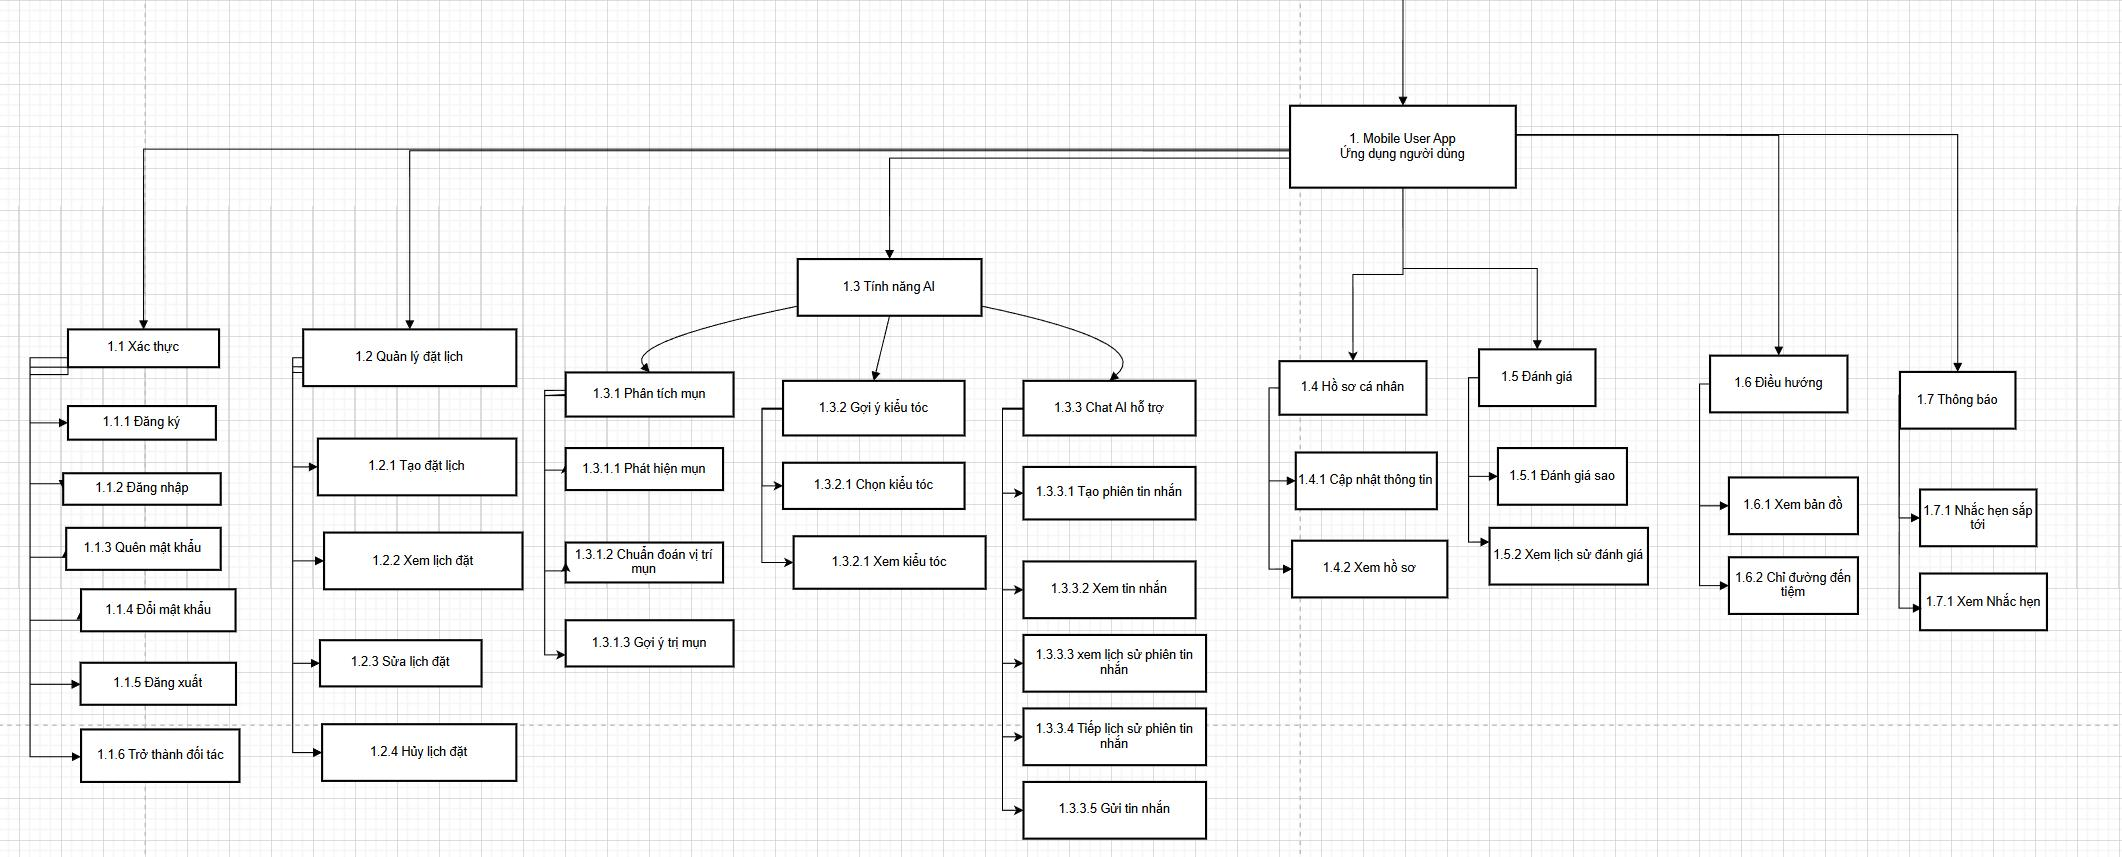
\includegraphics[width=0.8\textwidth]{figures/fdd_user.jpg}
    \caption{Phân rã chức năng theo app mobile người dùng}
    \label{fig:fdd_user}
\end{figure}

\subsubsection{Xác thực}
\begin{itemize}
    \item \textbf{Đăng ký tài khoản}
    \begin{itemize}
        \item Người dùng có thể tạo tài khoản mới bằng email, số điện thoại hoặc tài khoản mạng xã hội
        \item Hệ thống yêu cầu xác thực email/số điện thoại trước khi kích hoạt tài khoản
        \item Mật khẩu phải đáp ứng các tiêu chuẩn bảo mật (tối thiểu 8 ký tự, bao gồm chữ hoa, chữ thường, số và ký tự đặc biệt)
    \end{itemize}
    
    \item \textbf{Đăng nhập}
    \begin{itemize}
        \item Hỗ trợ đăng nhập bằng email/số điện thoại và mật khẩu
        \item Hỗ trợ đăng nhập bằng sinh trắc học (vân tay, Face ID)
        \item Tích hợp đăng nhập qua Google, Facebook, Apple ID
    \end{itemize}
    
    \item \textbf{Quên mật khẩu}
    \begin{itemize}
        \item Cho phép người dùng đặt lại mật khẩu qua email hoặc SMS
        \item Hệ thống gửi mã OTP để xác thực danh tính
    \end{itemize}
    
    \item \textbf{Đổi mật khẩu}
    \begin{itemize}
        \item Người dùng có thể thay đổi mật khẩu trong phần cài đặt tài khoản
        \item Yêu cầu xác thực mật khẩu cũ trước khi cho phép thay đổi
    \end{itemize}
    
    \item \textbf{Đăng xuất}
    \begin{itemize}
        \item Cho phép người dùng đăng xuất khỏi ứng dụng
        \item Xóa token xác thực và dữ liệu phiên làm việc
    \end{itemize}
    
    \item \textbf{Tích hợp đối tác}
    \begin{itemize}
        \item Hỗ trợ liên kết với các ứng dụng đối tác (ví điện tử, chương trình khách hàng thân thiết)
    \end{itemize}
\end{itemize}

\subsubsection{Quản lý đặt lịch}
\begin{itemize}
    \item \textbf{Tạo đặt lịch}
    \begin{itemize}
        \item Người dùng chọn salon, thợ cắt tóc, dịch vụ và thời gian mong muốn
        \item Hiển thị các khung giờ còn trống theo thời gian thực
        \item Cho phép thêm ghi chú đặc biệt cho cuộc hẹn
    \end{itemize}
    
    \item \textbf{Xem lịch đặt}
    \begin{itemize}
        \item Hiển thị danh sách các lịch hẹn đã đặt (quá khứ, hiện tại, tương lai)
        \item Phân loại theo trạng thái: đã xác nhận, đang chờ, đã hoàn thành, đã hủy
        \item Cung cấp bộ lọc và tìm kiếm lịch hẹn
    \end{itemize}
    
    \item \textbf{Sửa lịch đặt}
    \begin{itemize}
        \item Cho phép thay đổi thời gian, dịch vụ hoặc thợ cắt tóc
        \item Hiển thị cảnh báo nếu thay đổi ảnh hưởng đến giá cả hoặc thời gian chờ
        \item Yêu cầu xác nhận từ salon khi thay đổi lịch
    \end{itemize}
    
    \item \textbf{Hủy lịch đặt}
    \begin{itemize}
        \item Cho phép hủy lịch hẹn với lý do cụ thể
        \item Áp dụng chính sách hủy (miễn phí nếu hủy trước X giờ)
        \item Thông báo cho salon và thợ cắt tóc khi lịch hẹn bị hủy
    \end{itemize}
\end{itemize}

\subsubsection{Quản lý đặt lịch}
\begin{itemize}
    \item \textbf{Tạo đặt lịch}
    \begin{itemize}
        \item Phân tích hình dạng khuôn mặt từ ảnh người dùng upload
        \item Xác định các đặc điểm: hình dạng mặt, tỷ lệ khuôn mặt, đường nét
    \end{itemize}
    
    \item \textbf{Chuẩn đoán vi trị phân}
    \begin{itemize}
        \item Phân tích tình trạng da đầu và tóc từ hình ảnh
        \item Phát hiện các vấn đề: gàu, rụng tóc, tóc khô, tóc gãy
    \end{itemize}
    
    \item \textbf{Gợi ý kiểu tóc}
    \begin{itemize}
        \item Đề xuất các kiểu tóc phù hợp dựa trên hình dạng khuôn mặt
        \item Cân nhắc yếu tố: độ tuổi, giới tính, phong cách cá nhân
        \item Hiển thị hình ảnh minh họa cho mỗi kiểu tóc
    \end{itemize}
    
    \item \textbf{Chọn kiểu tóc}
    \begin{itemize}
        \item Cho phép người dùng lựa chọn kiểu tóc từ danh sách gợi ý
        \item Lưu kiểu tóc đã chọn vào hồ sơ người dùng
        \item Chia sẻ thông tin với thợ cắt tóc khi đặt lịch
    \end{itemize}
    
    \item \textbf{Xem kết quả}
    \begin{itemize}
        \item Hiển thị kết quả phân tích từ AI (hình dạng mặt, tình trạng tóc)
        \item So sánh ảnh trước và sau khi thử kiểu tóc (tính năng AR)
        \item Lưu lịch sử các lần phân tích
    \end{itemize}
    
    \item \textbf{Tạo phiên tư vấn}
    \begin{itemize}
        \item Khởi tạo phiên chat với AI chatbot để được tư vấn chi tiết
        \item Hỏi đáp về cách chăm sóc tóc, sản phẩm phù hợp
    \end{itemize}
    
    \item \textbf{Xem tin nhắn}
    \begin{itemize}
        \item Hiển thị lịch sử trò chuyện với AI chatbot
        \item Lưu trữ các gợi ý và lời khuyên từ AI
    \end{itemize}
    
    \item \textbf{Xem lịch sử phiên tư vấn}
    \begin{itemize}
        \item Truy cập các phiên tư vấn trước đó
        \item Theo dõi sự thay đổi của tình trạng tóc theo thời gian
    \end{itemize}
    
    \item \textbf{Tạo lịch sử phiên tư vấn}
    \begin{itemize}
        \item Tự động lưu mỗi phiên tư vấn với AI
        \item Gắn nhãn và phân loại theo chủ đề
    \end{itemize}
    
    \item \textbf{Gửi tin nhắn}
    \begin{itemize}
        \item Gửi câu hỏi và nhận phản hồi từ AI chatbot
        \item Hỗ trợ gửi hình ảnh để phân tích chi tiết hơn
    \end{itemize}
\end{itemize}

\subsubsection{Hồ sơ cá nhân}
\begin{itemize}
    \item \textbf{Cập nhật thông tin}
    \begin{itemize}
        \item Chỉnh sửa thông tin cá nhân: tên, số điện thoại, email, địa chỉ
        \item Upload và thay đổi ảnh đại diện
        \item Cập nhật sở thích và phong cách tóc yêu thích
    \end{itemize}
    
    \item \textbf{Xem hồ sơ}
    \begin{itemize}
        \item Hiển thị đầy đủ thông tin tài khoản
        \item Thống kê số lần sử dụng dịch vụ, điểm thưởng
        \item Xem lịch sử giao dịch và lịch hẹn
    \end{itemize}
\end{itemize}

\subsubsection{Đánh giá}
\begin{itemize}
    \item \textbf{Đánh giá sao}
    \begin{itemize}
        \item Đánh giá dịch vụ bằng thang điểm 1-5 sao
        \item Đánh giá riêng cho từng yếu tố: thợ cắt tóc, không gian, dịch vụ khách hàng
    \end{itemize}
    
    \item \textbf{Xem lịch sử đánh giá}
    \begin{itemize}
        \item Hiển thị các đánh giá đã gửi trước đó
        \item Cho phép chỉnh sửa hoặc xóa đánh giá trong thời gian cho phép
    \end{itemize}
\end{itemize}

\subsubsection{Điều hướng}
\begin{itemize}
    \item \textbf{Xem bản đồ}
    \begin{itemize}
        \item Hiển thị vị trí các salon trên bản đồ
        \item Tích hợp Google Maps hoặc Apple Maps
    \end{itemize}
    
    \item \textbf{Chỉ đường đến tiệm}
    \begin{itemize}
        \item Cung cấp hướng dẫn đường đi từ vị trí hiện tại đến salon
        \item Hiển thị thời gian di chuyển ước tính
        \item Hỗ trợ nhiều phương tiện: đi bộ, xe máy, ô tô, phương tiện công cộng
    \end{itemize}
\end{itemize}

\subsubsection{ Thông báo}
\begin{itemize}
    \item \textbf{Nhắc hẹn sắp tới}
    \begin{itemize}
        \item Gửi thông báo trước 24 giờ, 3 giờ và 30 phút trước lịch hẹn
        \item Cho phép người dùng tùy chỉnh thời gian nhắc nhở
    \end{itemize}
    
    \item \textbf{Xem nhắc hẹn}
    \begin{itemize}
        \item Hiển thị danh sách các thông báo nhắc hẹn
        \item Phân loại đã đọc và chưa đọc
    \end{itemize}
\end{itemize}

\subsection{Module 2: Mobile Barber App - Ứng dụng thợ cắt tóc}
\begin{figure}[H]
    \centering
    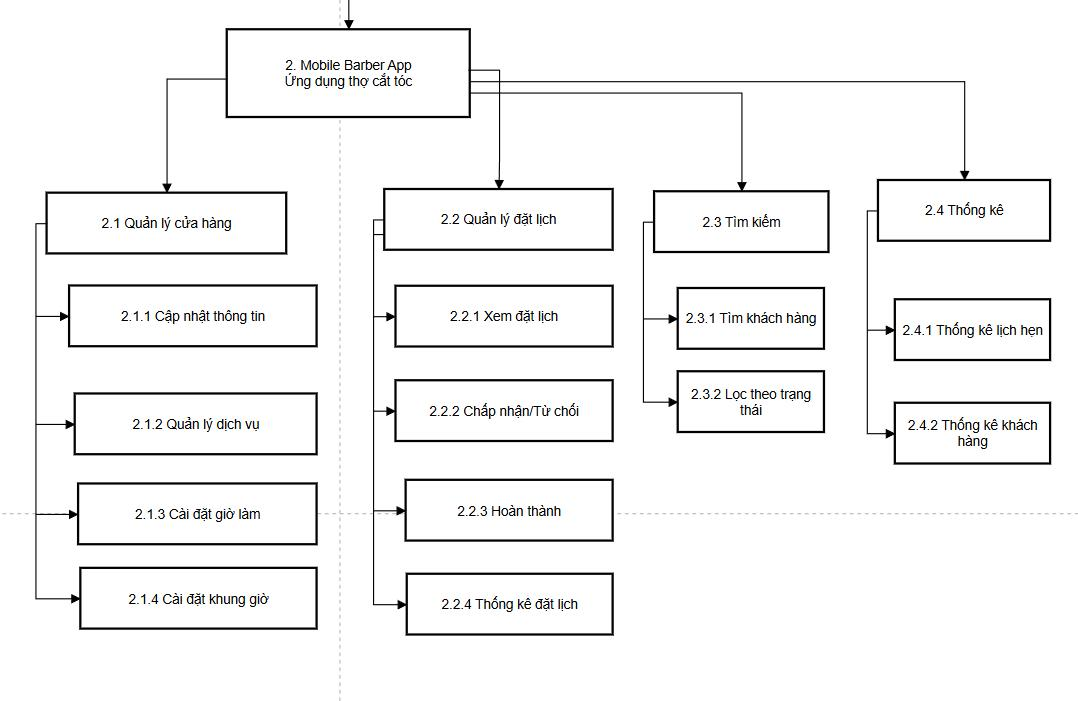
\includegraphics[width=0.8\textwidth]{figures/fdd_ower.jpg}
    \caption{Phân rã chức năng theo app mobile người thợ cắt tóc}
    \label{fig:fdd_ower}
\end{figure}
\subsubsection{ Quản lý cửa hàng}
\begin{itemize}
    \item \textbf{Cập nhật thông tin}
    \begin{itemize}
        \item Chỉnh sửa thông tin salon: tên, địa chỉ, số điện thoại
        \item Upload hình ảnh không gian salon
        \item Cập nhật giờ mở cửa và đóng cửa
    \end{itemize}
    
    \item \textbf{Quản lý dịch vụ}
    \begin{itemize}
        \item Thêm, sửa, xóa các dịch vụ cắt tóc
        \item Thiết lập giá cả và thời gian thực hiện cho mỗi dịch vụ
        \item Quản lý combo và gói dịch vụ
    \end{itemize}
    
    \item \textbf{Cài đặt giờ làm}
    \begin{itemize}
        \item Thiết lập lịch làm việc cho từng thợ cắt tóc
        \item Đánh dấu ngày nghỉ, ngày lễ
        \item Quản lý ca làm việc
    \end{itemize}
    
    \item \textbf{Cài đặt khung giờ}
    \begin{itemize}
        \item Định nghĩa các khung giờ đặt lịch (15 phút, 30 phút, 1 giờ)
        \item Thiết lập số lượng khách tối đa cho mỗi khung giờ
    \end{itemize}
\end{itemize}

\subsubsection{Quản lý đặt lịch}
\begin{itemize}
    \item \textbf{Xem đặt lịch}
    \begin{itemize}
        \item Hiển thị danh sách lịch hẹn theo ngày, tuần, tháng
        \item Lọc theo thợ cắt tóc, trạng thái, dịch vụ
        \item Xem chi tiết thông tin khách hàng và yêu cầu
    \end{itemize}
    
    \item \textbf{Chấp nhận/Từ chối}
    \begin{itemize}
        \item Xác nhận hoặc từ chối lịch hẹn của khách hàng
        \item Gửi thông báo cho khách hàng về trạng thái lịch hẹn
        \item Đưa ra lý do khi từ chối (nếu cần)
    \end{itemize}
    
    \item \textbf{Hoàn thành}
    \begin{itemize}
        \item Đánh dấu lịch hẹn đã hoàn thành
        \item Ghi nhận dịch vụ đã thực hiện
        \item Yêu cầu khách hàng đánh giá
    \end{itemize}
    
    \item \textbf{Thông kê đặt lịch}
    \begin{itemize}
        \item Xem báo cáo số lượng lịch hẹn theo thời gian
        \item Phân tích tỷ lệ hủy lịch, khách hàng quay lại
        \item Thống kê doanh thu từ lịch hẹn
    \end{itemize}
\end{itemize}

\subsubsection{Tìm kiếm}
\begin{itemize}
    \item \textbf{Tìm khách hàng}
    \begin{itemize}
        \item Tìm kiếm theo tên, số điện thoại, email
        \item Xem lịch sử sử dụng dịch vụ của khách hàng
    \end{itemize}
    
    \item \textbf{Lọc theo trạng thái}
    \begin{itemize}
        \item Lọc khách hàng theo: khách mới, khách thân thiết, khách VIP
        \item Lọc lịch hẹn theo trạng thái: chờ xác nhận, đã xác nhận, đã hoàn thành, đã hủy
    \end{itemize}
\end{itemize}

\subsubsection{Thống kê}
\begin{itemize}
    \item \textbf{Thống kê lịch hẹn}
    \begin{itemize}
        \item Báo cáo số lượng lịch hẹn theo ngày, tuần, tháng, năm
        \item Biểu đồ xu hướng đặt lịch
    \end{itemize}
    
    \item \textbf{Thống kê khách hàng}
    \begin{itemize}
        \item Số lượng khách hàng mới và khách hàng quay lại
        \item Phân tích độ tuổi, giới tính, sở thích của khách hàng
        \item Xác định nhóm khách hàng tiềm năng
    \end{itemize}
\end{itemize}

\subsection{Module 3: Web Admin Panel - Quản trị hệ thống}
\begin{figure}[H]
    \centering
    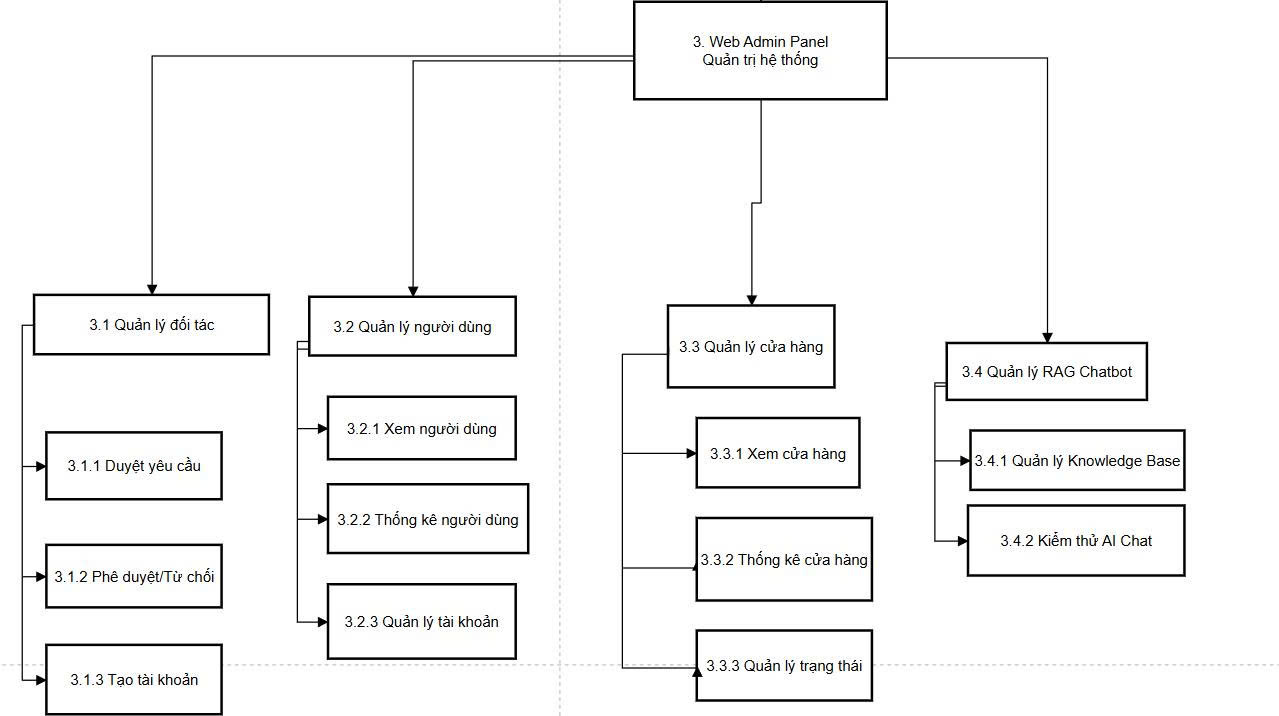
\includegraphics[width=0.8\textwidth]{figures/fdd_admin.jpg}
    \caption{Phân rã chức năng theo module web admin}
    \label{fig:fdd_admin}
\end{figure}
\subsubsection{Quản lý đối tác}
\begin{itemize}
    \item \textbf{Duyệt yêu cầu}
    \begin{itemize}
        \item Xem danh sách salon đăng ký làm đối tác
        \item Phê duyệt hoặc từ chối yêu cầu
        \item Gửi thông báo cho đối tác về kết quả
    \end{itemize}
    
    \item \textbf{Phê duyệt/Từ chối}
    \begin{itemize}
        \item Kiểm tra thông tin và giấy tờ pháp lý của đối tác
        \item Xác minh địa chỉ và thông tin liên hệ
    \end{itemize}
    
    \item \textbf{Tạo tài khoản}
    \begin{itemize}
        \item Tạo tài khoản quản trị cho salon đã được phê duyệt
        \item Gửi thông tin đăng nhập cho đối tác
    \end{itemize}
\end{itemize}

\subsubsection{ Quản lý người dùng}
\begin{itemize}
    \item \textbf{Xem người dùng}
    \begin{itemize}
        \item Hiển thị danh sách tất cả người dùng trong hệ thống
        \item Xem thông tin chi tiết của từng người dùng
    \end{itemize}
    
    \item \textbf{Thống kê người dùng}
    \begin{itemize}
        \item Báo cáo số lượng người dùng mới theo thời gian
        \item Phân tích tỷ lệ người dùng hoạt động/không hoạt động
        \item Thống kê theo vùng địa lý
    \end{itemize}
    
    \item \textbf{Quản lý tài khoản}
    \begin{itemize}
        \item Khóa/mở khóa tài khoản người dùng vi phạm
        \item Đặt lại mật khẩu cho người dùng
        \item Xóa tài khoản theo yêu cầu hoặc vi phạm chính sách
    \end{itemize}
\end{itemize}

\subsubsection{Quản lý cửa hàng}
\begin{itemize}
    \item \textbf{Xem cửa hàng}
    \begin{itemize}
        \item Hiển thị danh sách tất cả salon trong hệ thống
        \item Xem thông tin chi tiết, hình ảnh, dịch vụ của từng salon
    \end{itemize}
    
    \item \textbf{Thống kê cửa hàng}
    \begin{itemize}
        \item Báo cáo hiệu suất hoạt động của từng salon
        \item Xếp hạng salon theo đánh giá và doanh thu
    \end{itemize}
    
    \item \textbf{Quản lý trạng thái}
    \begin{itemize}
        \item Kích hoạt/vô hiệu hóa salon
        \item Tạm ngưng hoạt động đối với salon vi phạm
    \end{itemize}
\end{itemize}

\subsubsection{ Quản lý RAG Chatbot}
\begin{itemize}
    \item \textbf{Quản lý Knowledge Base}
    \begin{itemize}
        \item Thêm, sửa, xóa các câu hỏi thường gặp (FAQ)
        \item Cập nhật thông tin về dịch vụ, chính sách
        \item Quản lý cơ sở tri thức cho AI chatbot
    \end{itemize}
    
    \item \textbf{Thêm/Sửa/Xóa Documents}
    \begin{itemize}
        \item Upload tài liệu hướng dẫn, chính sách, quy định
        \item Chỉnh sửa nội dung tài liệu hiện có
        \item Xóa tài liệu không còn sử dụng
    \end{itemize}
    
    \item \textbf{Kiểm thử AI Chat}
    \begin{itemize}
        \item Giao diện test chatbot trước khi triển khai
        \item Đánh giá chất lượng phản hồi của AI
        \item Điều chỉnh và tối ưu hóa câu trả lời
    \end{itemize}
\end{itemize}

\section{Yêu cầu Phi chức năng}

\subsection{Hiệu năng (Performance)}
\begin{itemize}
    \item Thời gian phản hồi của ứng dụng không vượt quá 2 giây cho các thao tác thông thường
    \item API phải xử lý tối thiểu 1000 requests đồng thời
    \item Thời gian xử lý AI phân tích khuôn mặt không quá 5 giây
    \item Thời gian load danh sách lịch hẹn không quá 1 giây
    \item Trang web admin có thể hiển thị báo cáo với tối thiểu 100,000 bản ghi trong vòng 3 giây
\end{itemize}

\subsection{Khả năng mở rộng (Scalability)}
\begin{itemize}
    \item Hệ thống phải hỗ trợ tối thiểu 100,000 người dùng đồng thời
    \item Kiến trúc microservices để dễ dàng scale từng module độc lập
    \item Database phải hỗ trợ horizontal scaling
    \item Sử dụng CDN để phân phối nội dung tĩnh và giảm tải cho server
    \item Hỗ trợ auto-scaling dựa trên tải hệ thống
\end{itemize}

\subsection{Bảo mật (Security)}
\begin{itemize}
    \item Mã hóa dữ liệu nhạy cảm (mật khẩu, thông tin cá nhân) bằng AES-256
    \item Sử dụng HTTPS cho tất cả các kết nối
    \item Xác thực đa yếu tố (2FA) cho tài khoản admin và barber
    \item Token JWT có thời gian hết hạn và được làm mới định kỳ
    \item Chống tấn công SQL Injection, XSS, CSRF
    \item Backup dữ liệu hàng ngày và lưu trữ ở vị trí an toàn
    \item Tuân thủ các tiêu chuẩn bảo mật OWASP Top 10
    \item Giới hạn số lần đăng nhập sai để chống brute force attack
\end{itemize}

\subsection{Tính khả dụng (Availability)}
\begin{itemize}
    \item Hệ thống phải đảm bảo uptime 99.9\% (downtime tối đa 8.76 giờ/năm)
    \item Triển khai load balancer để phân phối tải và đảm bảo high availability
    \item Cơ chế failover tự động khi có sự cố
    \item Monitoring và alerting 24/7 để phát hiện sự cố sớm
    \item Kế hoạch disaster recovery với RTO < 4 giờ và RPO < 1 giờ
\end{itemize}

\subsection{Khả năng bảo trì (Maintainability)}
\begin{itemize}
    \item Code phải tuân thủ coding standards và best practices
    \item Tài liệu kỹ thuật đầy đủ cho từng module
    \item Sử dụng version control (Git) với quy trình branching rõ ràng
    \item Automated testing với coverage tối thiểu 80\%
\end{itemize}


\section{Sơ đồ use case }
\subsection{Sơ đồ use case tổng quát}
\begin{figure}[H]
    \centering
    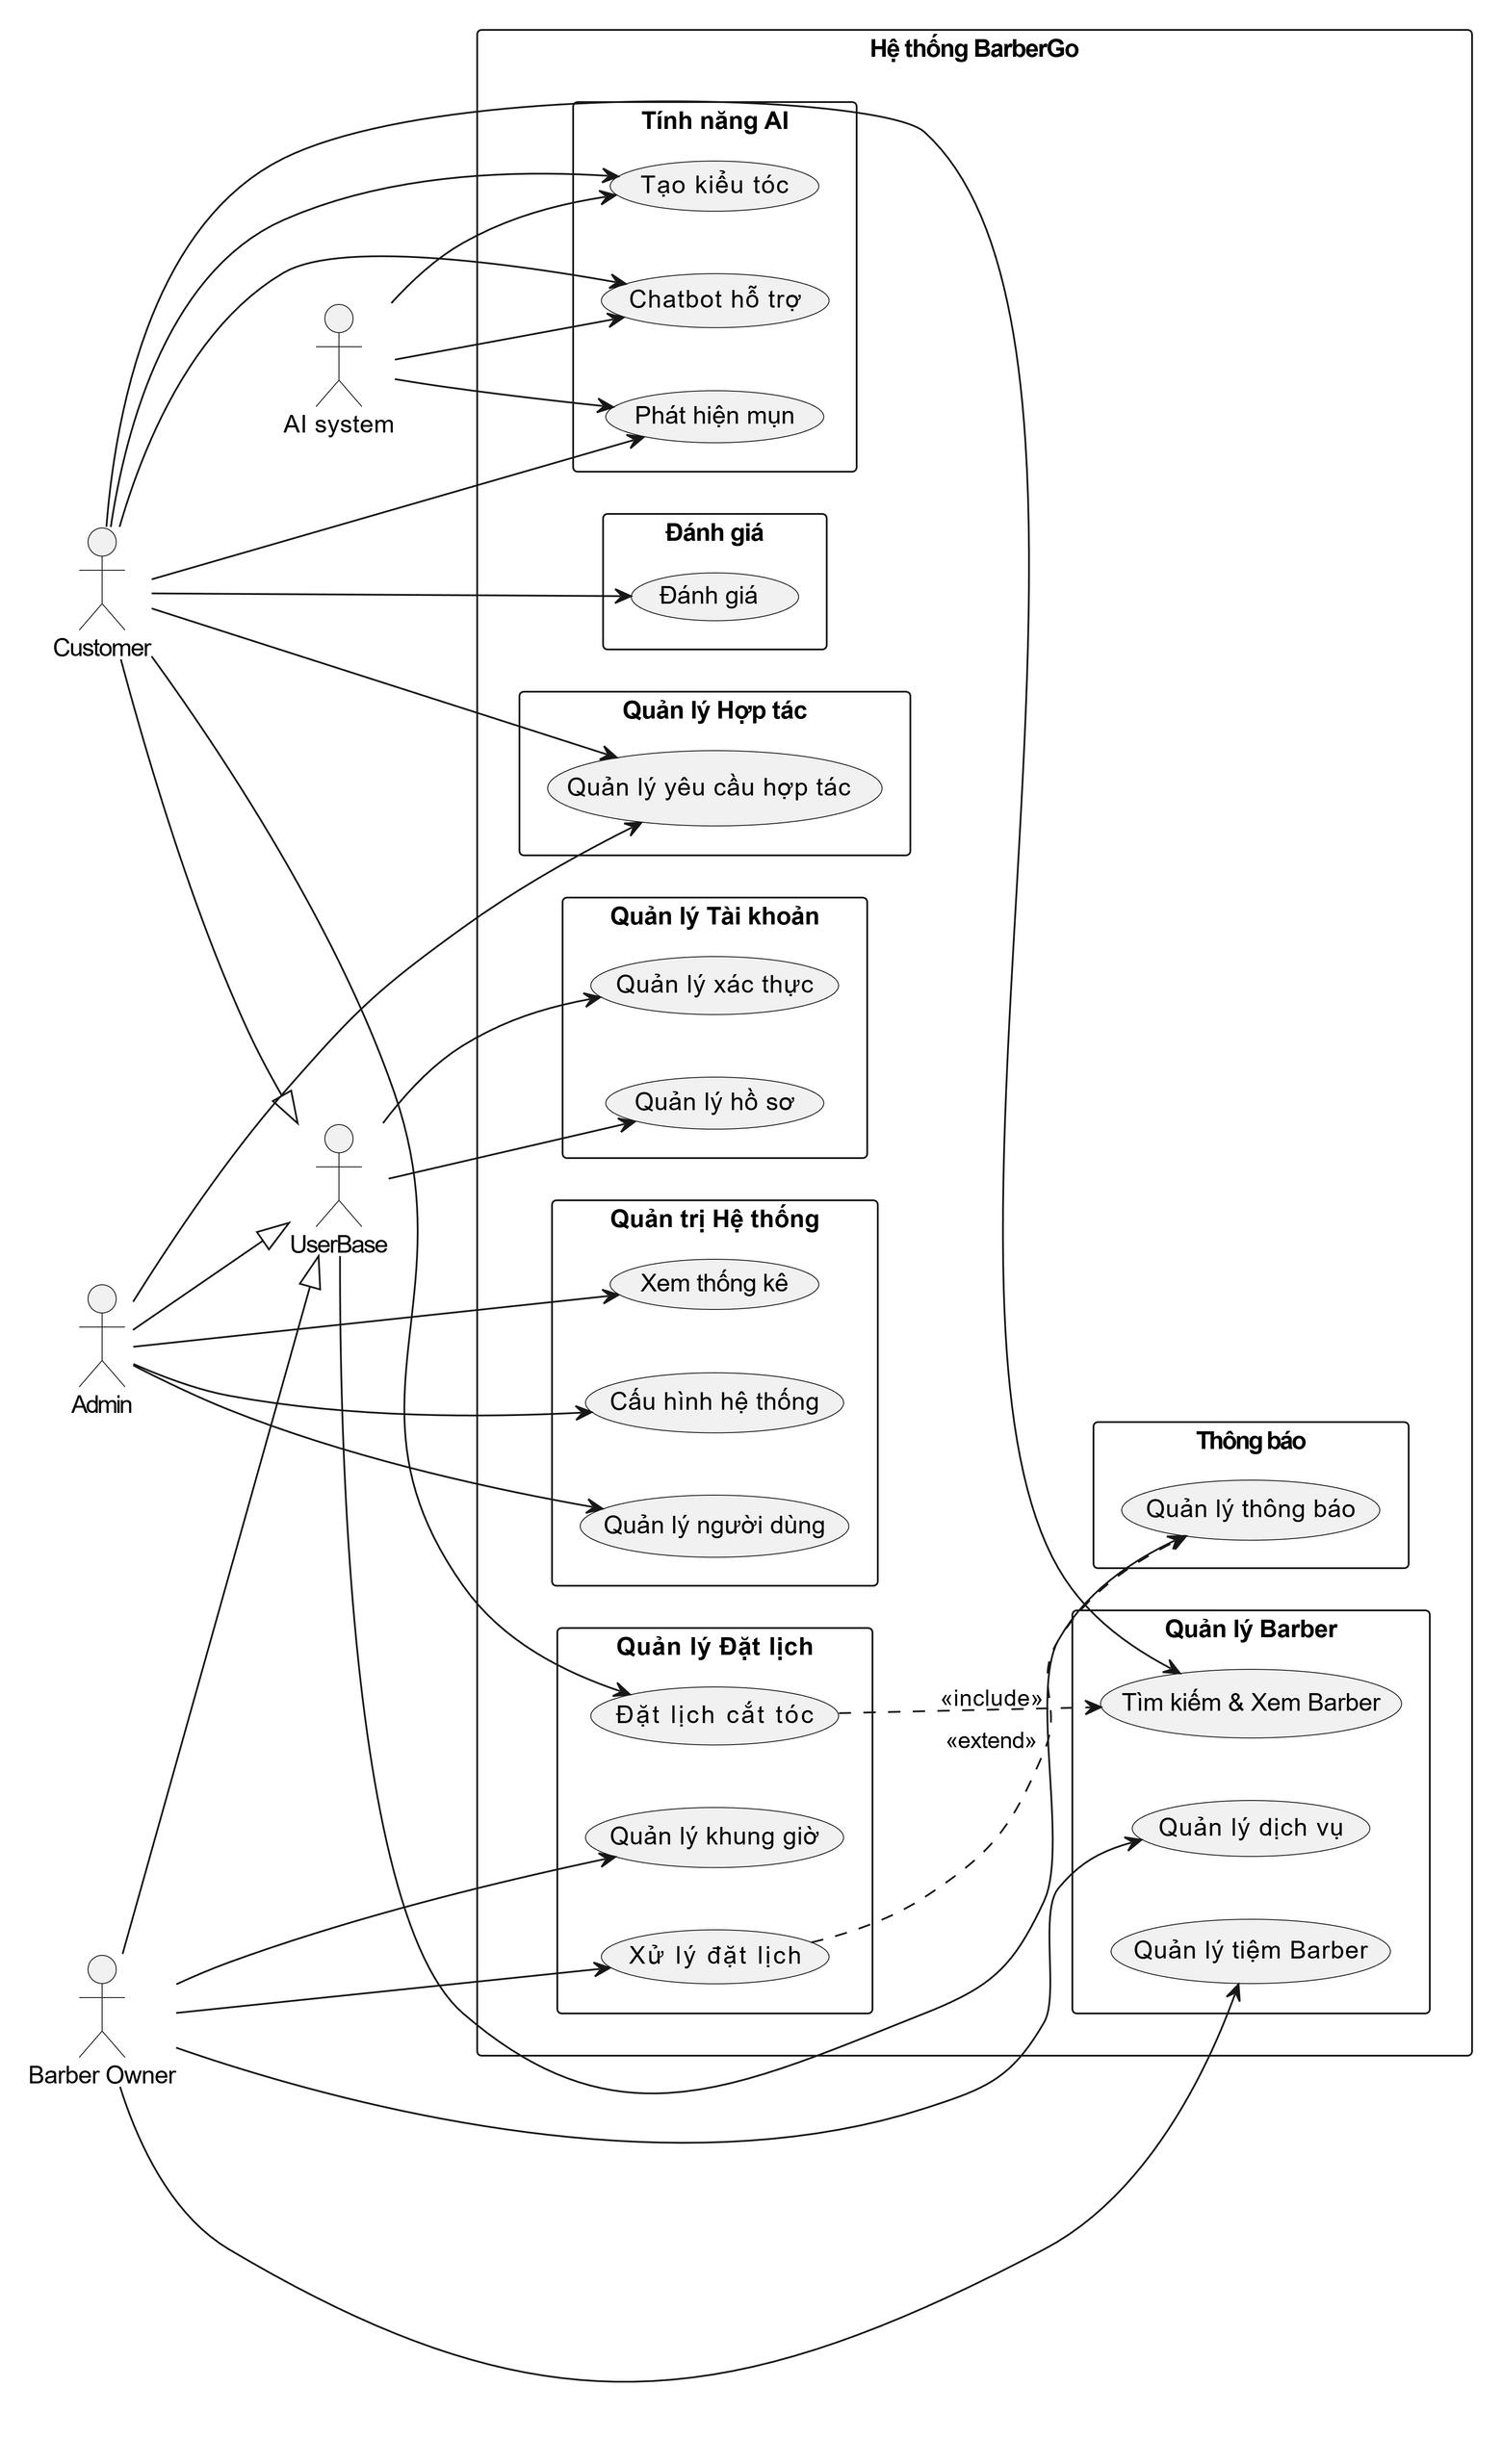
\includegraphics[width=0.7\textwidth]{figures/usecase_tq.jpg}
    \caption{Sơ đồ use case tổng quát}
    \label{fig:usecase_overall}
\end{figure}
Các Actor trong Hệ thống bao gồm:
\begin{itemize}[noitemsep]
    \item Customer (Khách hàng): Người dùng cuối sử dụng ứng dụng mobile để đặt lịch cắt tóc, nhận gợi ý kiểu tóc và tư vấn chăm sóc tóc thông qua hệ thống AI.

    \item Barber Owner (Chủ tiệm cắt tóc): Chủ salon hoặc người quản lý sử dụng ứng dụng mobile để quản lý cửa hàng, dịch vụ, thợ cắt tóc và xử lý các lịch hẹn của khách hàng.

    \item Admin (Quản trị viên): Người quản trị hệ thống sử dụng web admin panel để quản lý người dùng, salon, cấu hình hệ thống và giám sát hoạt động của AI chatbot.

    \item AI System (Hệ thống AI): Hệ thống trí tuệ nhân tạo tự động hỗ trợ khách hàng thông qua phân tích khuôn mặt, gợi ý kiểu tóc và chatbot tư vấn.
\end{itemize}
%----------------------------------------------------------------Đăng nhập đăng ký---------------
\subsection{Sơ đồ use case chi tiết về xử lý đăng nhập đăng ký}
\begin{figure}[H]
    \centering
    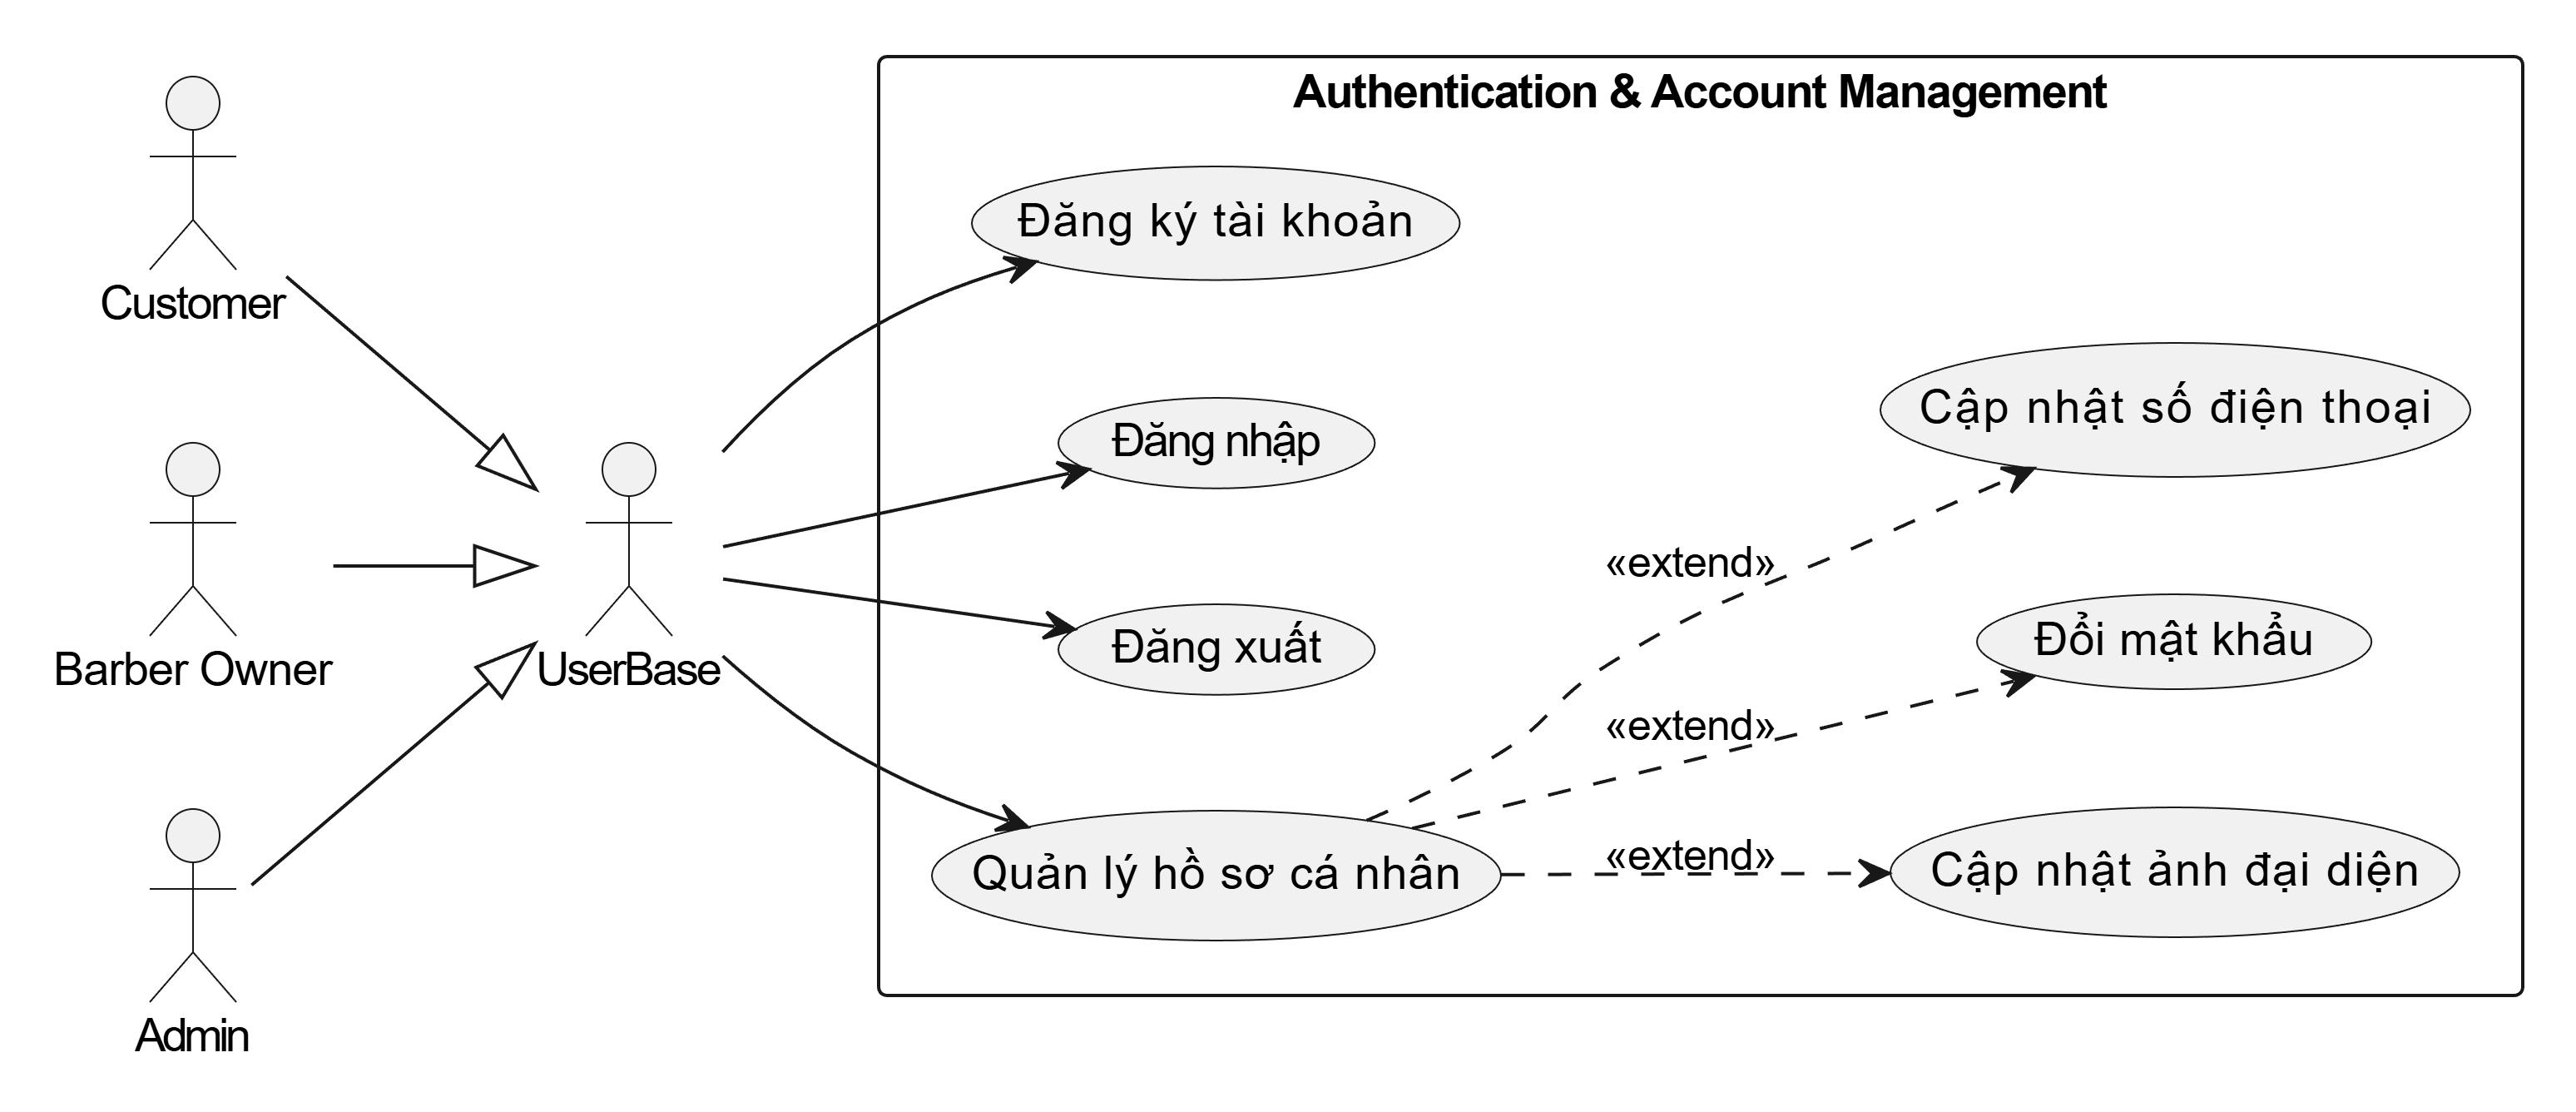
\includegraphics[width=0.8\textwidth]{figures/usecase_authen.jpg}
    \caption{Sơ đồ use case người dùng đăng nhập đăng ký}
    \label{fig:usecase_user}
\end{figure}
Dưới đây là các đặc tả use case của người dùng đăng nhập đăng ký.


\begin{table}[H]
\centering
\caption{Đặc tả Use Case UC-01: Đăng ký tài khoản}
\label{tab:uc01}
\begin{tabular}{|p{4cm}|p{11cm}|}
\hline
\textbf{Actor} & Customer, Barber Owner \\
\hline
\textbf{Mô tả} & Người dùng tạo tài khoản mới \\
\hline
\textbf{Tiền điều kiện} & Chưa có tài khoản \\
\hline
\textbf{Luồng chính} & 
1. Nhập thông tin (email/SĐT, mật khẩu, họ tên) \newline
2. Hệ thống xác thực thông tin \newline
3. Gửi mã OTP qua email/SMS \newline
4. Nhập mã OTP \newline
5. Tạo tài khoản thành công \\
\hline
\textbf{Luồng phụ} & 
2a. Thông tin không hợp lệ $\rightarrow$ Hiển thị lỗi \newline
4a. OTP sai/hết hạn $\rightarrow$ Gửi lại OTP \\
\hline
\textbf{Hậu điều kiện} & Tài khoản được tạo và kích hoạt \\
\hline
\end{tabular}
\end{table}



\begin{table}[H]
\centering
\caption{Đặc tả Use Case UC-02: Đăng nhập}
\label{tab:uc02}
\begin{tabular}{|p{4cm}|p{11cm}|}
\hline
\textbf{Actor} & Customer, Barber Owner, Admin \\
\hline
\textbf{Mô tả} & Đăng nhập vào hệ thống \\
\hline
\textbf{Tiền điều kiện} & Có tài khoản hợp lệ \\
\hline
\textbf{Luồng chính} & 
1. Nhập email/SĐT và mật khẩu \newline
2. Hệ thống xác thực \newline
3. Cấp token truy cập \newline
4. Chuyển đến màn hình chính \\
\hline
\textbf{Luồng phụ} & 
2a. Sai thông tin đăng nhập $\rightarrow$ Thông báo lỗi \newline
2b. Tài khoản bị khóa $\rightarrow$ Thông báo liên hệ admin \newline
Extend: Đăng nhập bằng sinh trắc học, mạng xã hội \\
\hline
\textbf{Hậu điều kiện} & Người dùng truy cập được hệ thống \\
\hline
\end{tabular}
\end{table}



\begin{table}[H]
\centering
\caption{Đặc tả Use Case UC-03: Đăng xuất}
\label{tab:uc03}
\begin{tabular}{|p{4cm}|p{11cm}|}
\hline
\textbf{Actor} & Customer, Barber Owner, Admin \\
\hline
\textbf{Mô tả} & Thoát khỏi hệ thống \\
\hline
\textbf{Luồng chính} & 
1. Chọn đăng xuất \newline
2. Xóa token và session \newline
3. Chuyển về màn hình đăng nhập \\
\hline
\textbf{Hậu điều kiện} & Phiên làm việc kết thúc \\
\hline
\end{tabular}
\end{table}



\begin{table}[H]
\centering
\caption{Đặc tả Use Case UC-04: Quản lý hồ sơ cá nhân}
\label{tab:uc04}
\begin{tabular}{|p{4cm}|p{11cm}|}
\hline
\textbf{Actor} & Customer, Barber Owner \\
\hline
\textbf{Mô tả} & Xem và cập nhật thông tin cá nhân \\
\hline
\textbf{Luồng chính} & 
1. Truy cập hồ sơ cá nhân \newline
2. Xem thông tin hiện tại \newline
3. Chỉnh sửa thông tin (tên, SĐT, ảnh đại diện) \newline
4. Lưu thay đổi \newline
5. Hệ thống cập nhật thành công \\
\hline
\textbf{Luồng phụ} & 
Extend: Cập nhật số điện thoại (yêu cầu xác thực OTP) \newline
Extend: Đổi mật khẩu (yêu cầu mật khẩu cũ) \newline
Extend: Cập nhật ảnh đại diện \\
\hline
\textbf{Hậu điều kiện} & Thông tin cá nhân được cập nhật \\
\hline
\end{tabular}
\end{table}

%----------------------------------------------------------------booking---------------
\begin{figure}[H]
    \centering
    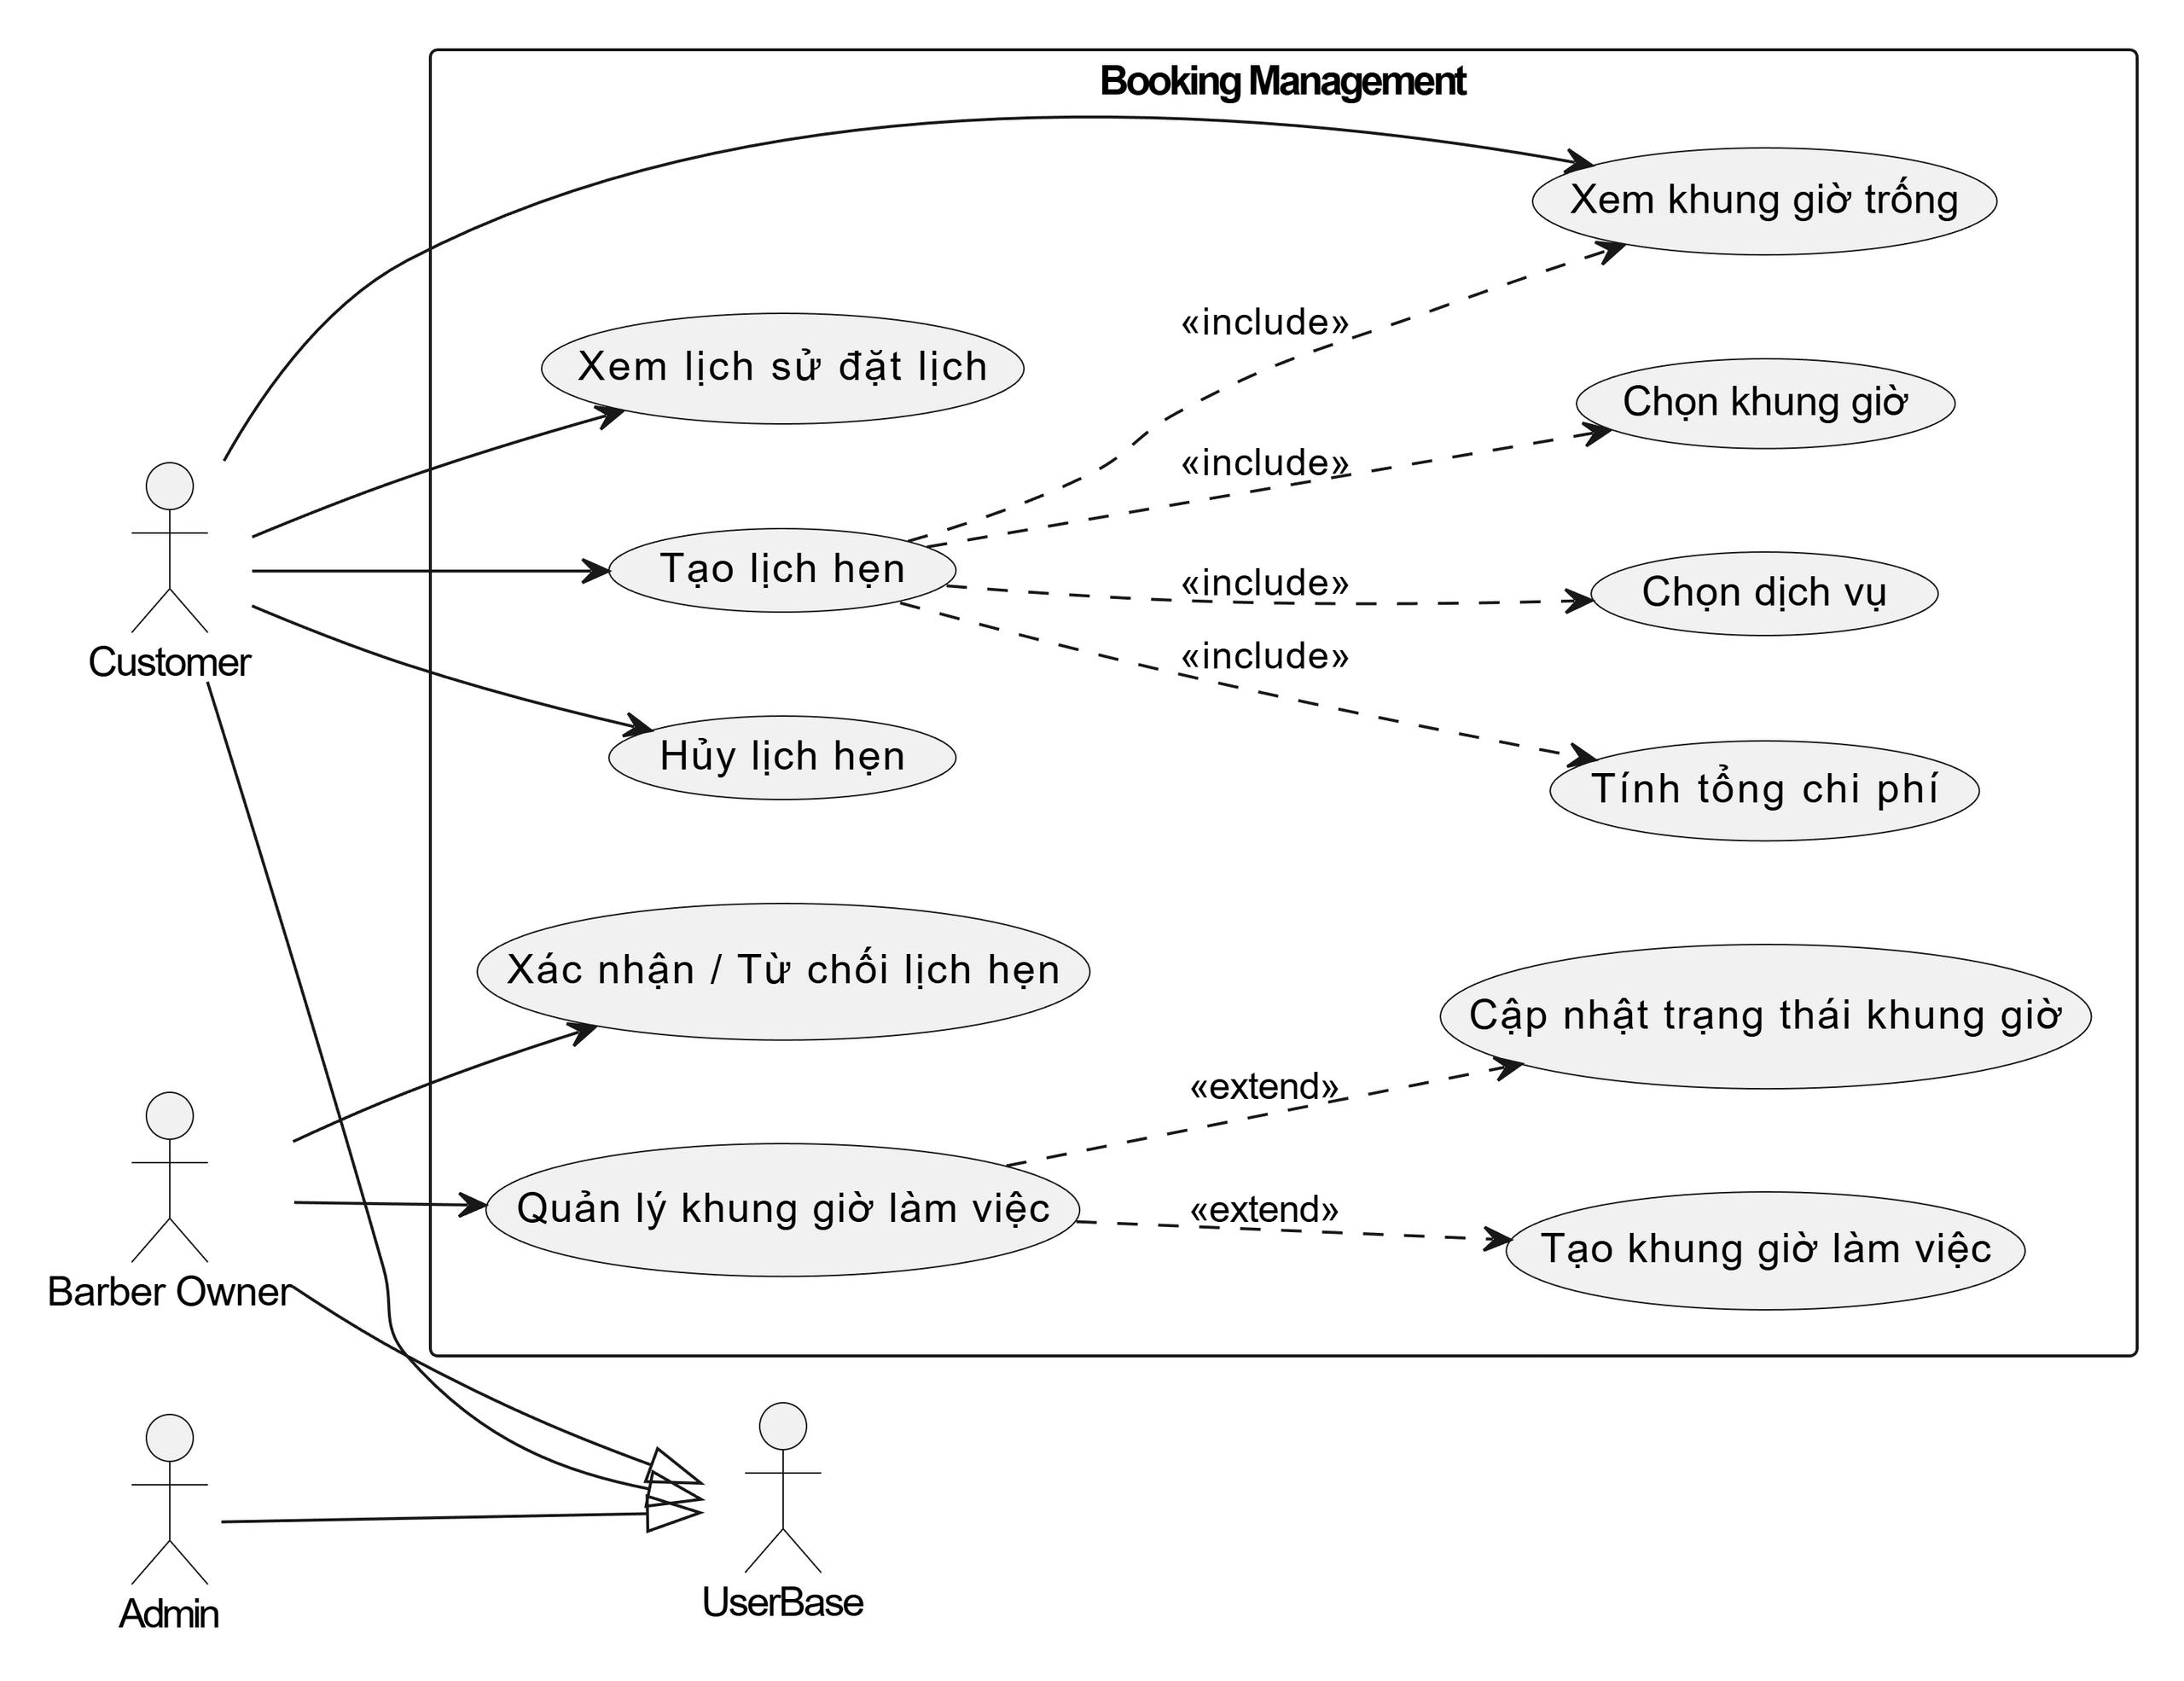
\includegraphics[width=0.8\textwidth]{figures/usecase_booking.jpg}
    \caption{Sơ đồ use case người dùng đặt lịch}
    \label{fig:usecase_booking}
\end{figure}
Dưới đây là các đặc tả use case của người dùng đặt lịch cắt tóc.

\begin{table}[H]
\centering
\caption{Đặc tả Use Case UC-05: Xem lịch sử đặt lịch}
\label{tab:uc05}
\begin{tabular}{|p{4cm}|p{11cm}|}
\hline
\textbf{Actor} & Customer \\
\hline
\textbf{Mô tả} & Xem các lịch hẹn đã đặt \\
\hline
\textbf{Luồng chính} & 
1. Truy cập lịch sử đặt lịch \newline
2. Hiển thị danh sách lịch hẹn (quá khứ, hiện tại, tương lai) \newline
3. Xem chi tiết lịch hẹn \\
\hline
\textbf{Luồng phụ} & 
Include: Xem khung giờ trống \newline
Lọc theo trạng thái, ngày, salon \\
\hline
\textbf{Hậu điều kiện} & Không có \\
\hline
\end{tabular}
\end{table}


\begin{table}[H]
\centering
\caption{Đặc tả Use Case UC-06: Tạo lịch hẹn}
\label{tab:uc06}
\begin{tabular}{|p{4cm}|p{11cm}|}
\hline
\textbf{Actor} & Customer \\
\hline
\textbf{Mô tả} & Đặt lịch cắt tóc mới \\
\hline
\textbf{Tiền điều kiện} & Đã đăng nhập \\
\hline
\textbf{Luồng chính} & 
1. Chọn salon và thợ cắt tóc \newline
2. Include: Xem khung giờ trống \newline
3. Include: Chọn khung giờ \newline
4. Include: Chọn dịch vụ \newline
5. Include: Tính tổng chi phí \newline
6. Xác nhận đặt lịch \newline
7. Hệ thống tạo lịch hẹn và thông báo cho barber \\
\hline
\textbf{Luồng phụ} & 
2a. Không có khung giờ trống $\rightarrow$ Chọn ngày khác \newline
6a. Hủy đặt lịch \\
\hline
\textbf{Hậu điều kiện} & Lịch hẹn được tạo, trạng thái ``Chờ xác nhận'' \\
\hline
\end{tabular}
\end{table}


\begin{table}[H]
\centering
\caption{Đặc tả Use Case UC-07: Hủy lịch hẹn}
\label{tab:uc07}
\begin{tabular}{|p{4cm}|p{11cm}|}
\hline
\textbf{Actor} & Customer \\
\hline
\textbf{Mô tả} & Hủy lịch hẹn đã đặt \\
\hline
\textbf{Tiền điều kiện} & Có lịch hẹn chưa hoàn thành \\
\hline
\textbf{Luồng chính} & 
1. Chọn lịch hẹn cần hủy \newline
2. Chọn lý do hủy \newline
3. Xác nhận hủy \newline
4. Hệ thống cập nhật trạng thái ``Đã hủy'' \newline
5. Thông báo cho barber owner \\
\hline
\textbf{Luồng phụ} & 
3a. Hủy quá muộn $\rightarrow$ Áp dụng phí hủy lịch \\
\hline
\textbf{Hậu điều kiện} & Lịch hẹn bị hủy, khung giờ được giải phóng \\
\hline
\end{tabular}
\end{table}


\begin{table}[H]
\centering
\caption{Đặc tả Use Case UC-08: Xác nhận/Từ chối lịch hẹn}
\label{tab:uc08}
\begin{tabular}{|p{4cm}|p{11cm}|}
\hline
\textbf{Actor} & Barber Owner \\
\hline
\textbf{Mô tả} & Xử lý yêu cầu đặt lịch từ khách hàng \\
\hline
\textbf{Tiền điều kiện} & Có lịch hẹn chờ xác nhận \\
\hline
\textbf{Luồng chính} & 
1. Xem danh sách lịch hẹn chờ xác nhận \newline
2. Xem chi tiết lịch hẹn \newline
3. Chấp nhận hoặc từ chối \newline
4. Extend: Cập nhật trạng thái khung giờ \newline
5. Gửi thông báo cho customer \\
\hline
\textbf{Luồng phụ} & 
3a. Từ chối $\rightarrow$ Nhập lý do từ chối \\
\hline
\textbf{Hậu điều kiện} & Lịch hẹn được xác nhận hoặc từ chối \\
\hline
\end{tabular}
\end{table}


\begin{table}[H]
\centering
\caption{Đặc tả Use Case UC-09: Quản lý khung giờ làm việc}
\label{tab:uc09}
\begin{tabular}{|p{4cm}|p{11cm}|}
\hline
\textbf{Actor} & Barber Owner \\
\hline
\textbf{Mô tả} & Thiết lập lịch làm việc cho salon \\
\hline
\textbf{Luồng chính} & 
1. Truy cập quản lý khung giờ \newline
2. Extend: Tạo khung giờ làm việc (giờ mở/đóng cửa, ca làm) \newline
3. Đánh dấu ngày nghỉ/lễ \newline
4. Lưu cấu hình \\
\hline
\textbf{Hậu điều kiện} & Khung giờ được cập nhật \\
\hline
\end{tabular}
\end{table}

%----------------------------------------------------------------AI---------------
\begin{figure}[H]
    \centering
    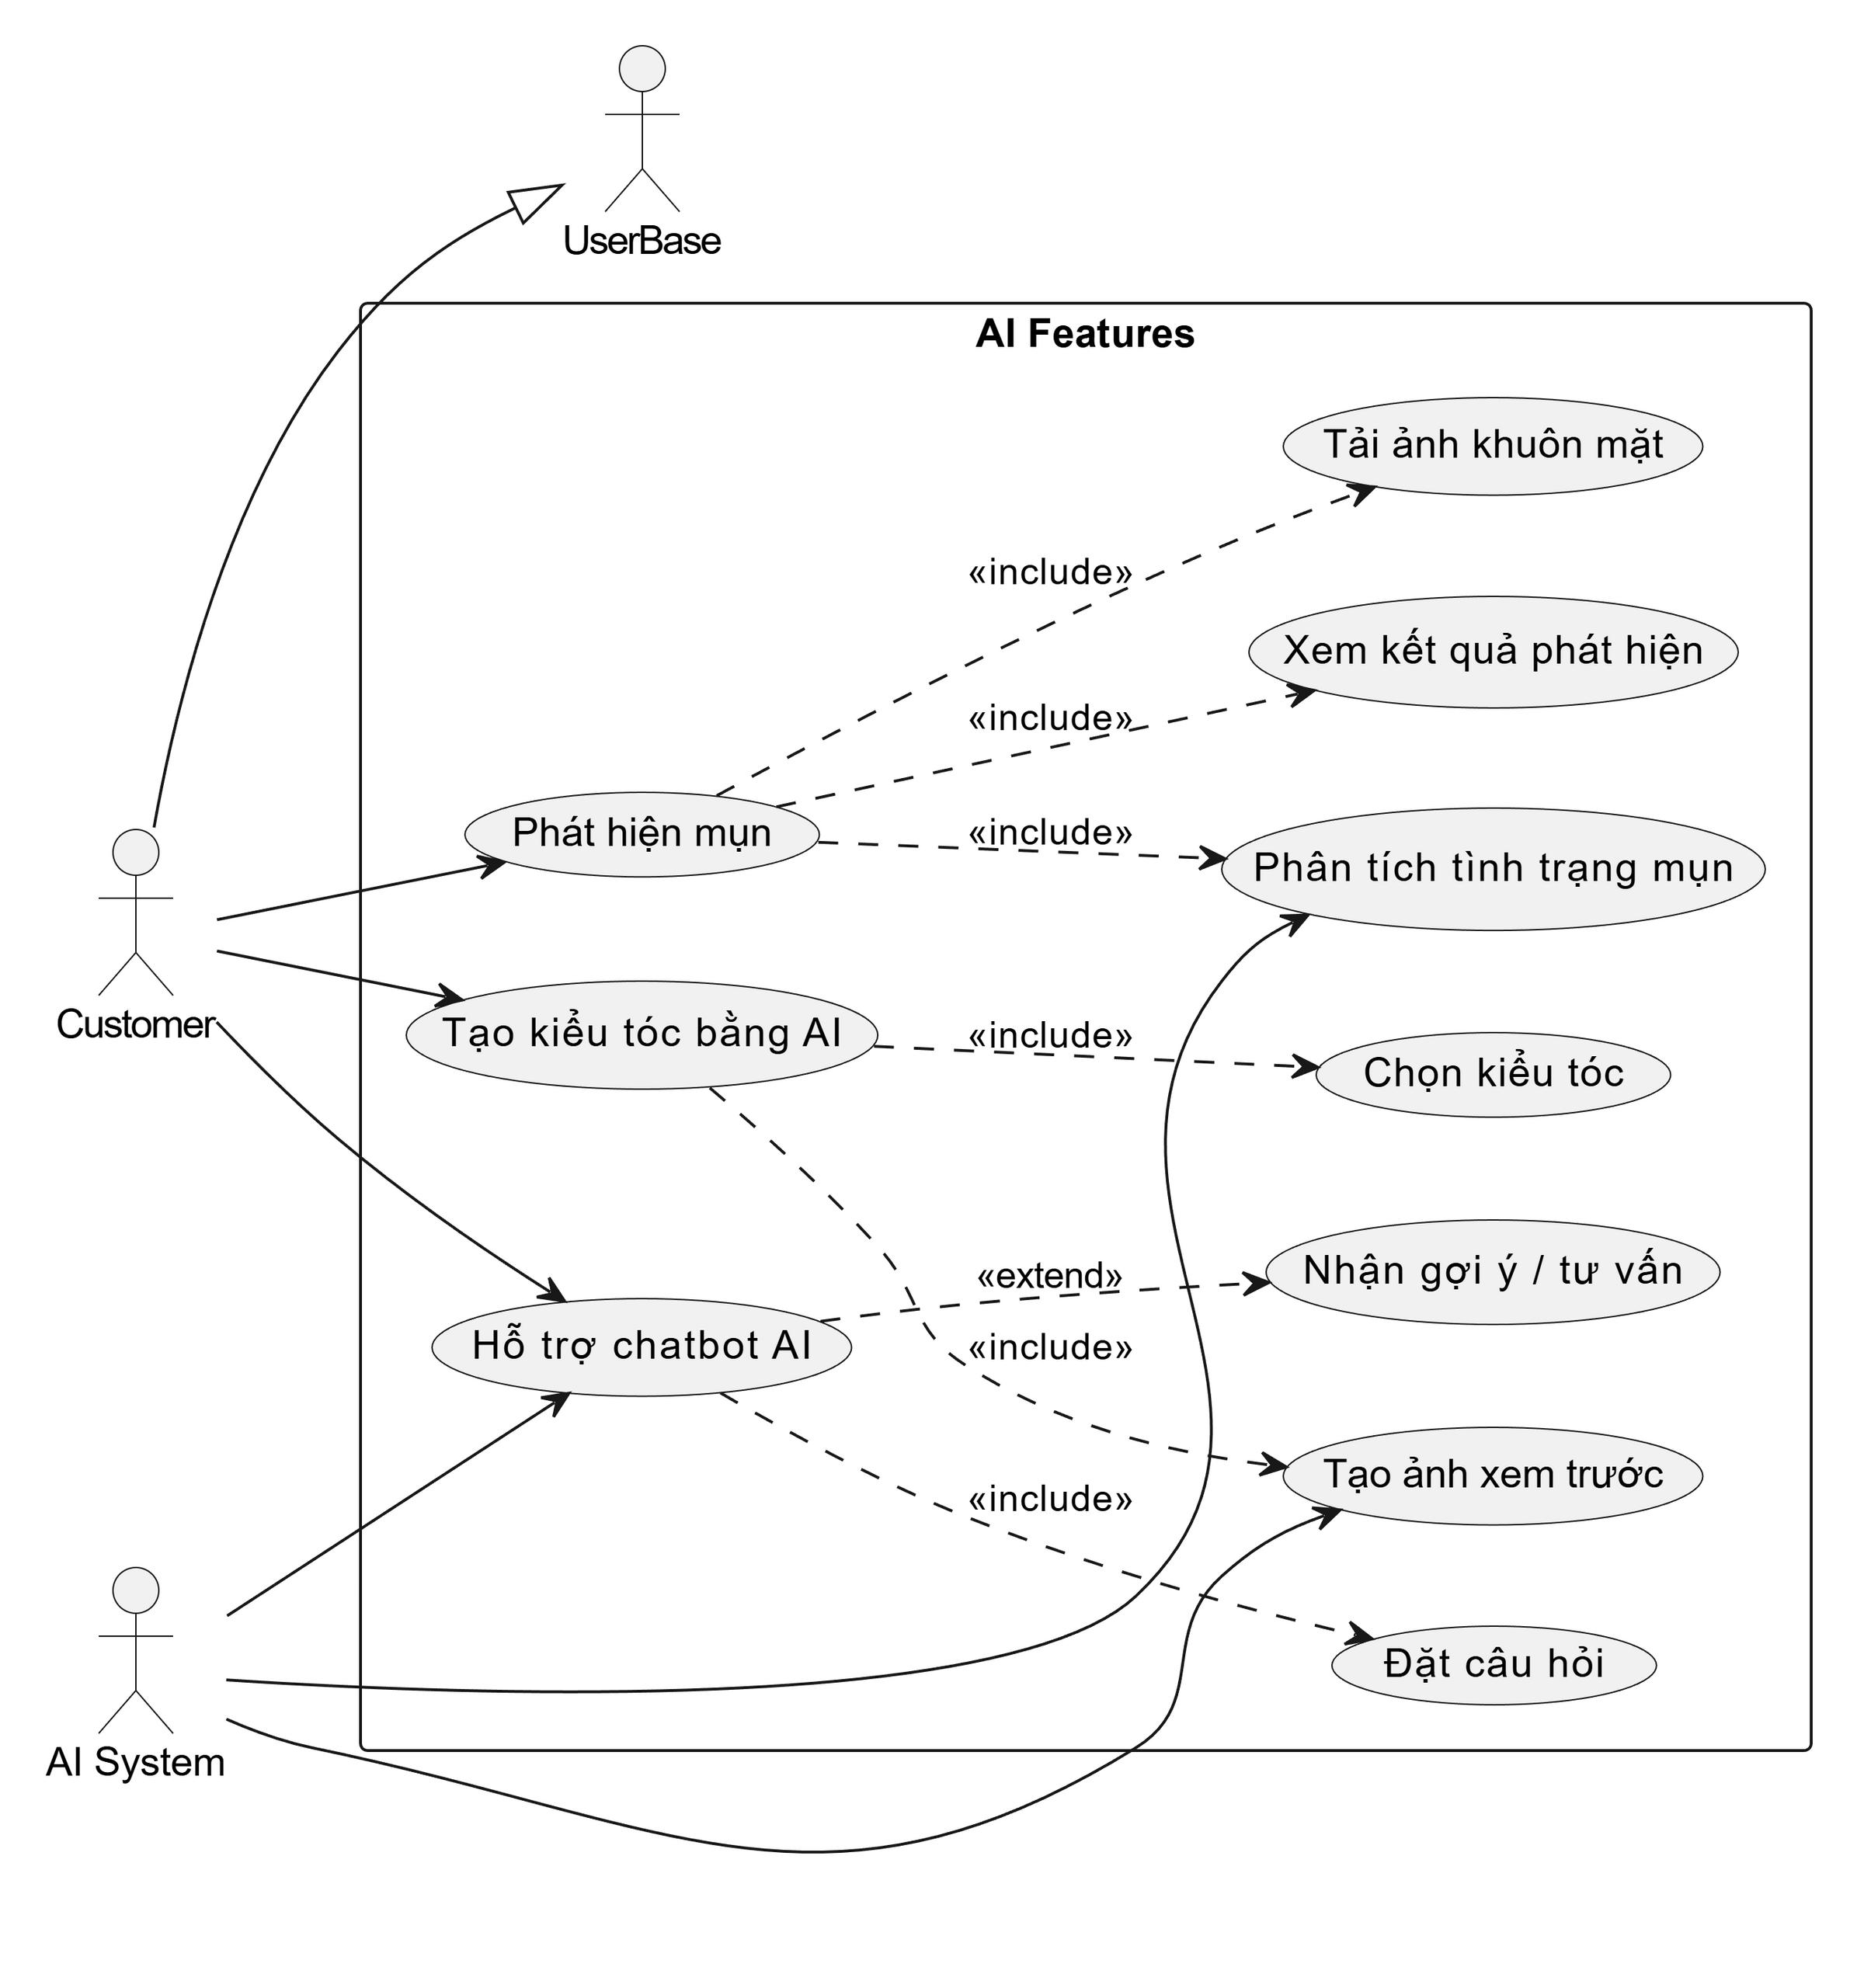
\includegraphics[width=1.0\textwidth]{figures/usecase_AI.jpg}
    \caption{Sơ đồ use case người dùng sử dụng dịch vụ AI}
    \label{fig:usecase_AI}
\end{figure}
Dưới đây là các đặc tả use case của người dùng sử dụng dịch vụ AI phân tích khuôn mặt, gợi ý kiểu tóc và hỏi đáp.


\begin{table}[H]
\centering
\caption{Đặc tả Use Case UC-16: Phát hiện mụn}
\label{tab:uc16}
\begin{tabular}{|p{4cm}|p{11cm}|}
\hline
\textbf{Actor} & Customer, AI System \\
\hline
\textbf{Mô tả} & Phân tích tình trạng da mặt \\
\hline
\textbf{Tiền điều kiện} & Đã đăng nhập \\
\hline
\textbf{Luồng chính} & 
1. Upload ảnh khuôn mặt \newline
2. Include: Tải ảnh khuôn mặt \newline
3. AI phân tích hình ảnh \newline
4. Include: Xem kết quả phát hiện \newline
5. Include: Phân tích tình trạng mụn (loại, vị trí, mức độ) \newline
6. Hiển thị kết quả và đề xuất chăm sóc \\
\hline
\textbf{Hậu điều kiện} & Kết quả được lưu vào hồ sơ \\
\hline
\end{tabular}
\end{table}

\begin{table}[H]
\centering
\caption{Đặc tả Use Case UC-17: Tạo kiểu tóc bằng AI}
\label{tab:uc17}
\begin{tabular}{|p{4cm}|p{11cm}|}
\hline
\textbf{Actor} & Customer, AI System \\
\hline
\textbf{Mô tả} & Gợi ý kiểu tóc phù hợp \\
\hline
\textbf{Tiền điều kiện} & Đã upload ảnh khuôn mặt \\
\hline
\textbf{Luồng chính} & 
1. AI phân tích hình dạng khuôn mặt \newline
2. Include: Chọn kiểu tóc \newline
3. Hiển thị danh sách kiểu tóc phù hợp \newline
4. Customer chọn kiểu tóc yêu thích \newline
5. Extend: Nhận gợi ý/tư vấn \newline
6. Include: Tạo ảnh xem trước (AR) \\
\hline
\textbf{Luồng phụ} & 
Include: Đặt câu hỏi với chatbot về kiểu tóc \\
\hline
\textbf{Hậu điều kiện} & Kiểu tóc được lưu, có thể dùng khi đặt lịch \\
\hline
\end{tabular}
\end{table}


\begin{table}[H]
\centering
\caption{Đặc tả Use Case UC-18: Hỗ trợ Chatbot AI}
\label{tab:uc18}
\begin{tabular}{|p{4cm}|p{11cm}|}
\hline
\textbf{Actor} & Customer, AI System \\
\hline
\textbf{Mô tả} & Tư vấn qua chatbot AI \\
\hline
\textbf{Luồng chính} & 
1. Mở chatbot \newline
2. Extend: Nhận gợi ý/tư vấn \newline
3. Include: Tạo ảnh xem trước (nếu hỏi về kiểu tóc) \newline
4. Include: Đặt câu hỏi \newline
5. AI trả lời dựa trên Knowledge Base \newline
6. Lưu lịch sử hội thoại \\
\hline
\textbf{Hậu điều kiện} & Phiên tư vấn được lưu \\
\hline
\end{tabular}
\end{table}
%----------------------------------------------------------------Tiệm tóc quản lý---------------
\begin{figure}[H]
    \centering
    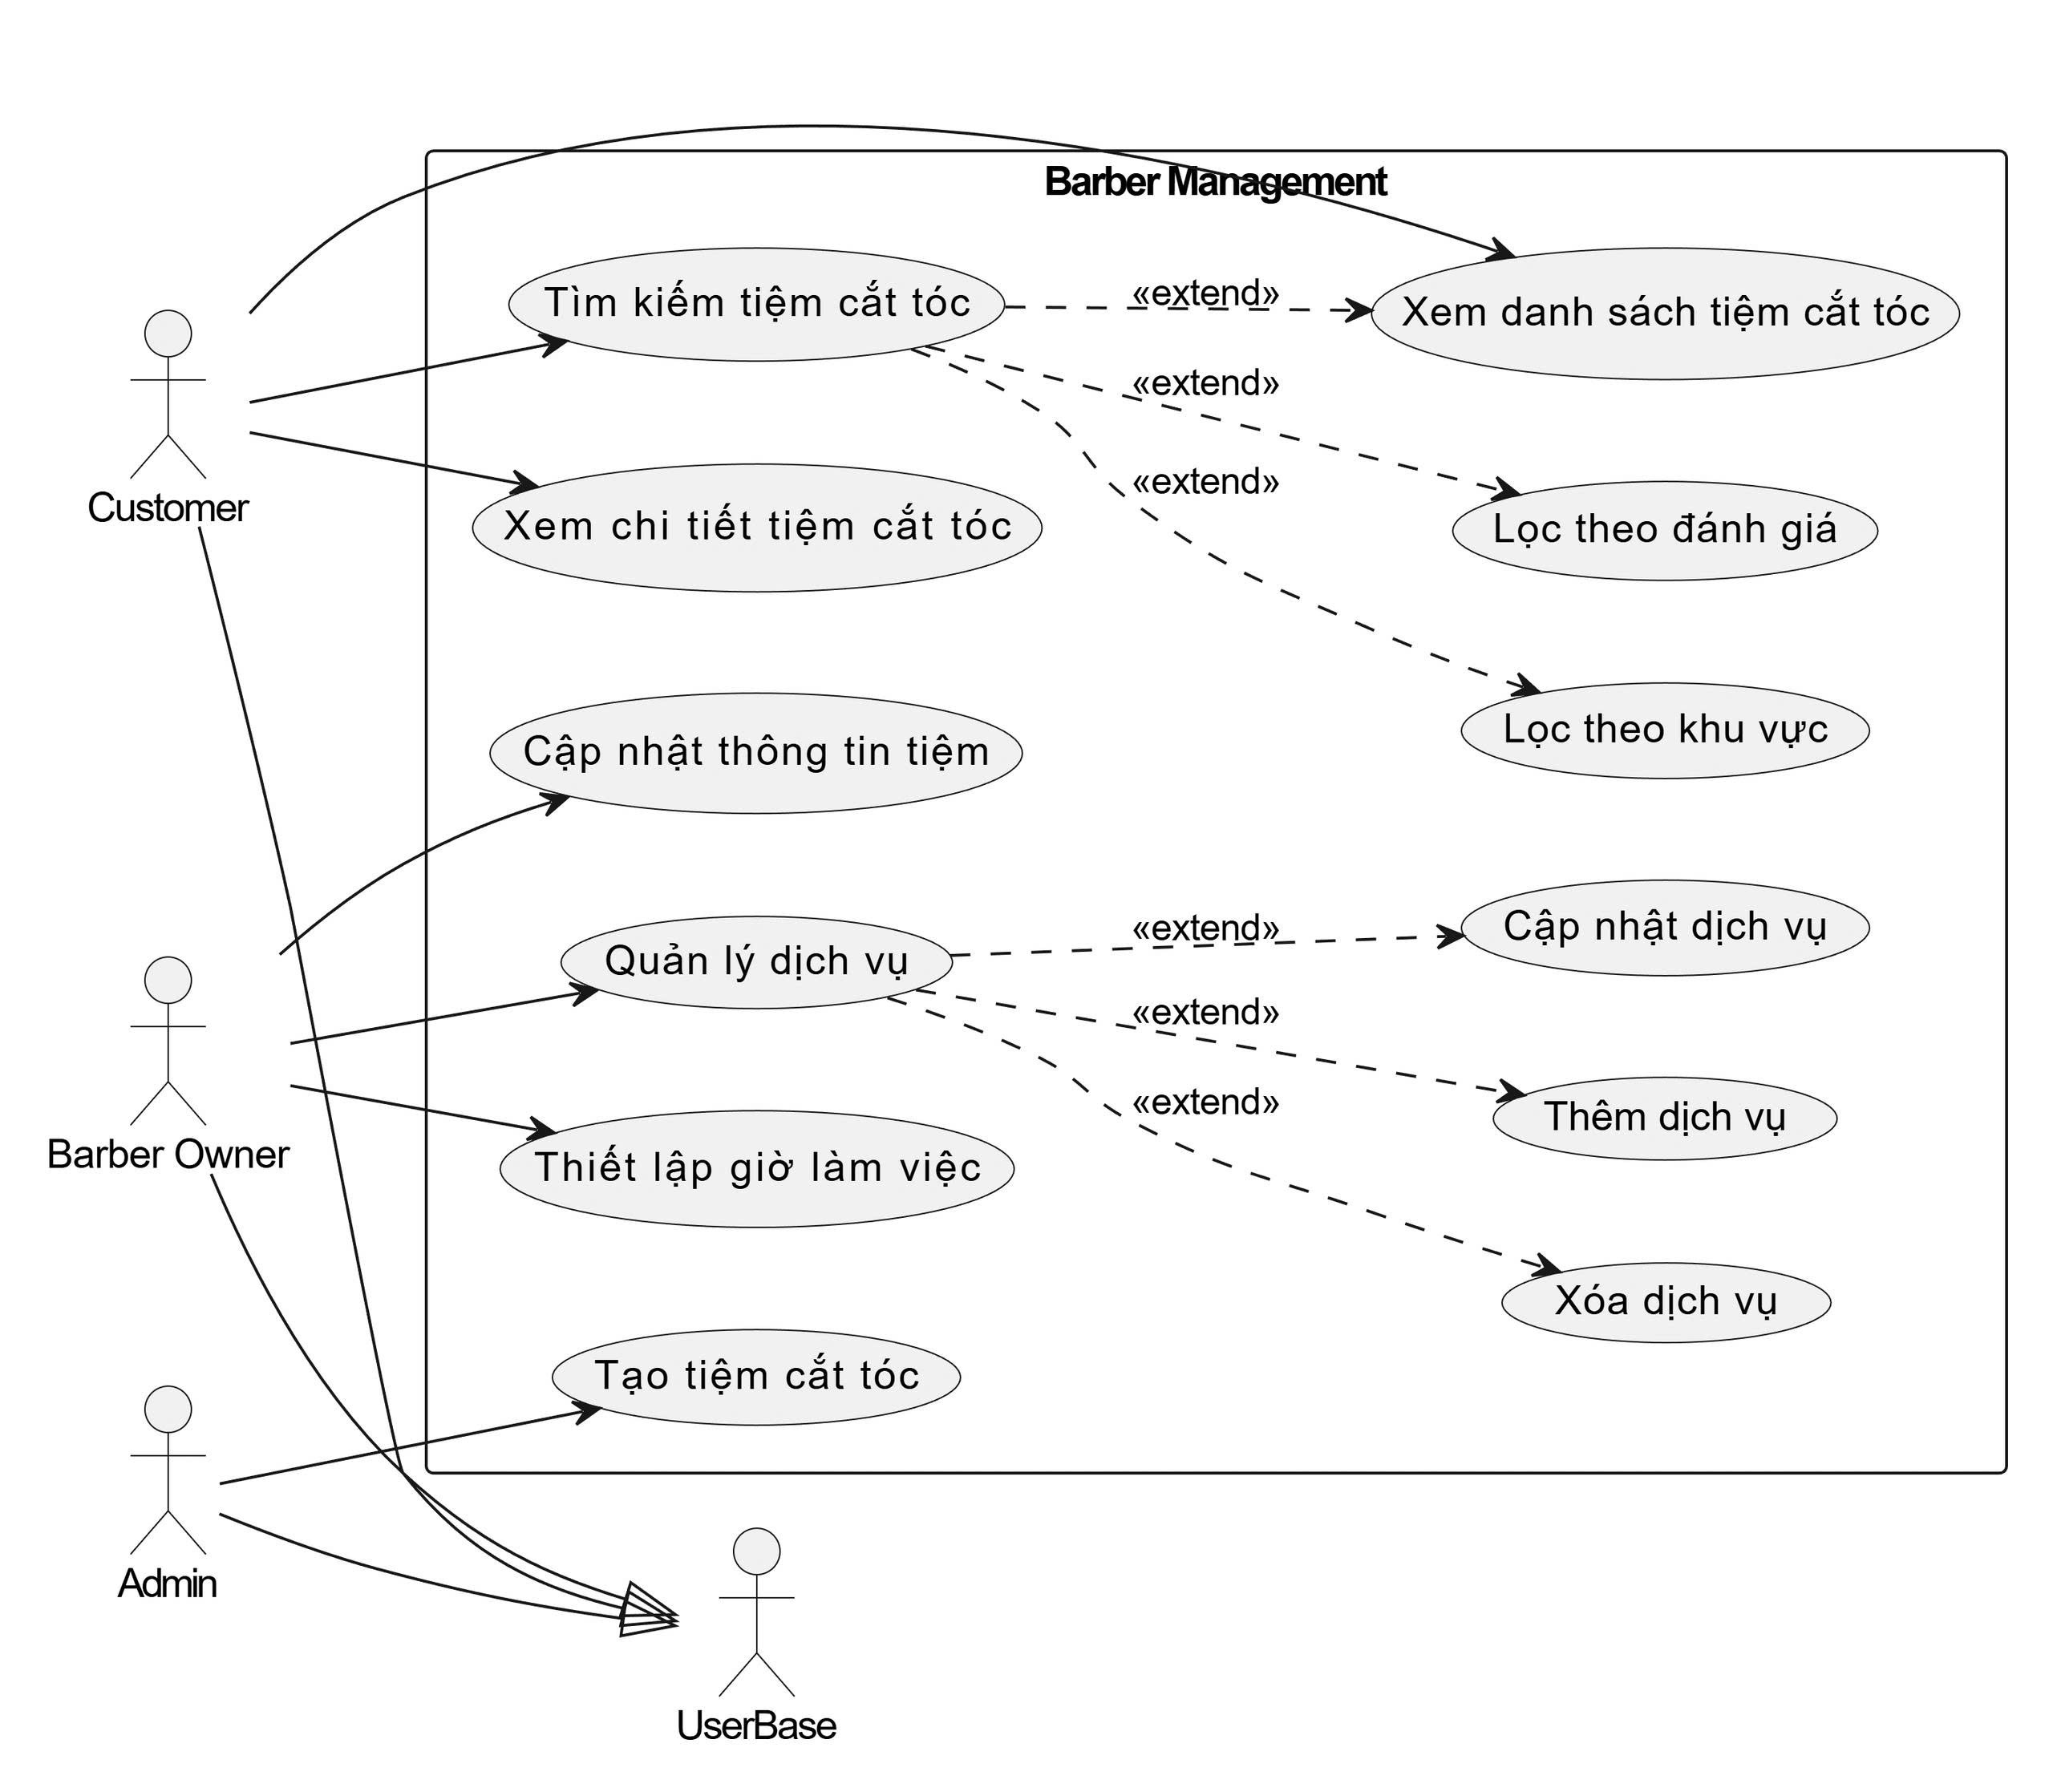
\includegraphics[width=1.0\textwidth]{figures/usecase_manager.jpg}
    \caption{Sơ đồ use case người thợ cắt tóc quản lý cửa hàng và đặt lịch}
    \label{fig:usecase_manager}
\end{figure}

Dưới đây là các đặc tả use case của người thợ cắt tóc quản lý cửa hàng và đặt lịch.

\begin{table}[H]
\centering
\caption{Đặc tả Use Case UC-10: Xem chi tiết tiệm cắt tóc}
\label{tab:uc10}
\begin{tabular}{|p{4cm}|p{11cm}|}
\hline
\textbf{Actor} & Customer \\
\hline
\textbf{Mô tả} & Xem thông tin salon \\
\hline
\textbf{Luồng chính} & 
1. Chọn salon \newline
2. Hiển thị thông tin (địa chỉ, giờ làm, dịch vụ, đánh giá, hình ảnh) \newline
3. Xem danh sách thợ cắt tóc \\
\hline
\textbf{Hậu điều kiện} & Không có \\
\hline
\end{tabular}
\end{table}


\begin{table}[H]
\centering
\caption{Đặc tả Use Case UC-11: Tìm kiếm tiệm cắt tóc}
\label{tab:uc11}
\begin{tabular}{|p{4cm}|p{11cm}|}
\hline
\textbf{Actor} & Customer \\
\hline
\textbf{Mô tả} & Tìm salon theo tiêu chí \\
\hline
\textbf{Luồng chính} & 
1. Nhập từ khóa tìm kiếm \newline
2. Extend: Xem danh sách tiệm cắt tóc \newline
3. Extend: Lọc theo đánh giá \newline
4. Extend: Lọc theo khu vực \newline
5. Hiển thị kết quả phù hợp \\
\hline
\textbf{Hậu điều kiện} & Không có \\
\hline
\end{tabular}
\end{table}


\begin{table}[H]
\centering
\caption{Đặc tả Use Case UC-12: Tạo tiệm cắt tóc}
\label{tab:uc12}
\begin{tabular}{|p{4cm}|p{11cm}|}
\hline
\textbf{Actor} & Barber Owner \\
\hline
\textbf{Mô tả} & Đăng ký salon mới \\
\hline
\textbf{Tiền điều kiện} & Đã đăng nhập với vai trò Barber Owner \\
\hline
\textbf{Luồng chính} & 
1. Nhập thông tin salon (tên, địa chỉ, SĐT, giấy phép KD) \newline
2. Upload hình ảnh salon \newline
3. Gửi yêu cầu đến Admin \newline
4. Chờ phê duyệt \\
\hline
\textbf{Hậu điều kiện} & Yêu cầu tạo salon được gửi \\
\hline
\end{tabular}
\end{table}


\begin{table}[H]
\centering
\caption{Đặc tả Use Case UC-13: Cập nhật thông tin tiệm}
\label{tab:uc13}
\begin{tabular}{|p{4cm}|p{11cm}|}
\hline
\textbf{Actor} & Barber Owner \\
\hline
\textbf{Mô tả} & Chỉnh sửa thông tin salon \\
\hline
\textbf{Luồng chính} & 
1. Truy cập quản lý tiệm \newline
2. Chỉnh sửa thông tin \newline
3. Extend: Cập nhật dịch vụ (thêm/xóa/sửa) \newline
4. Lưu thay đổi \\
\hline
\textbf{Hậu điều kiện} & Thông tin salon được cập nhật \\
\hline
\end{tabular}
\end{table}


\begin{table}[H]
\centering
\caption{Đặc tả Use Case UC-14: Quản lý dịch vụ}
\label{tab:uc14}
\begin{tabular}{|p{4cm}|p{11cm}|}
\hline
\textbf{Actor} & Barber Owner \\
\hline
\textbf{Mô tả} & Quản lý danh sách dịch vụ của salon \\
\hline
\textbf{Luồng chính} & 
1. Truy cập quản lý dịch vụ \newline
2. Extend: Thêm dịch vụ mới (tên, giá, thời gian) \newline
3. Extend: Xóa dịch vụ \\
\hline
\textbf{Hậu điều kiện} & Danh sách dịch vụ được cập nhật \\
\hline
\end{tabular}
\end{table}


\begin{table}[H]
\centering
\caption{Đặc tả Use Case UC-15: Thiết lập giờ làm việc}
\label{tab:uc15}
\begin{tabular}{|p{4cm}|p{11cm}|}
\hline
\textbf{Actor} & Barber Owner \\
\hline
\textbf{Mô tả} & Cấu hình giờ mở/đóng cửa \\
\hline
\textbf{Luồng chính} & 
1. Thiết lập giờ làm việc cho từng ngày \newline
2. Đánh dấu ngày nghỉ \newline
3. Lưu cấu hình \\
\hline
\textbf{Hậu điều kiện} & Lịch làm việc được cập nhật \\
\hline
\end{tabular}
\end{table}
%----------------------------------------------------------------Hợp tác---------------

\begin{figure}[H]
    \centering
    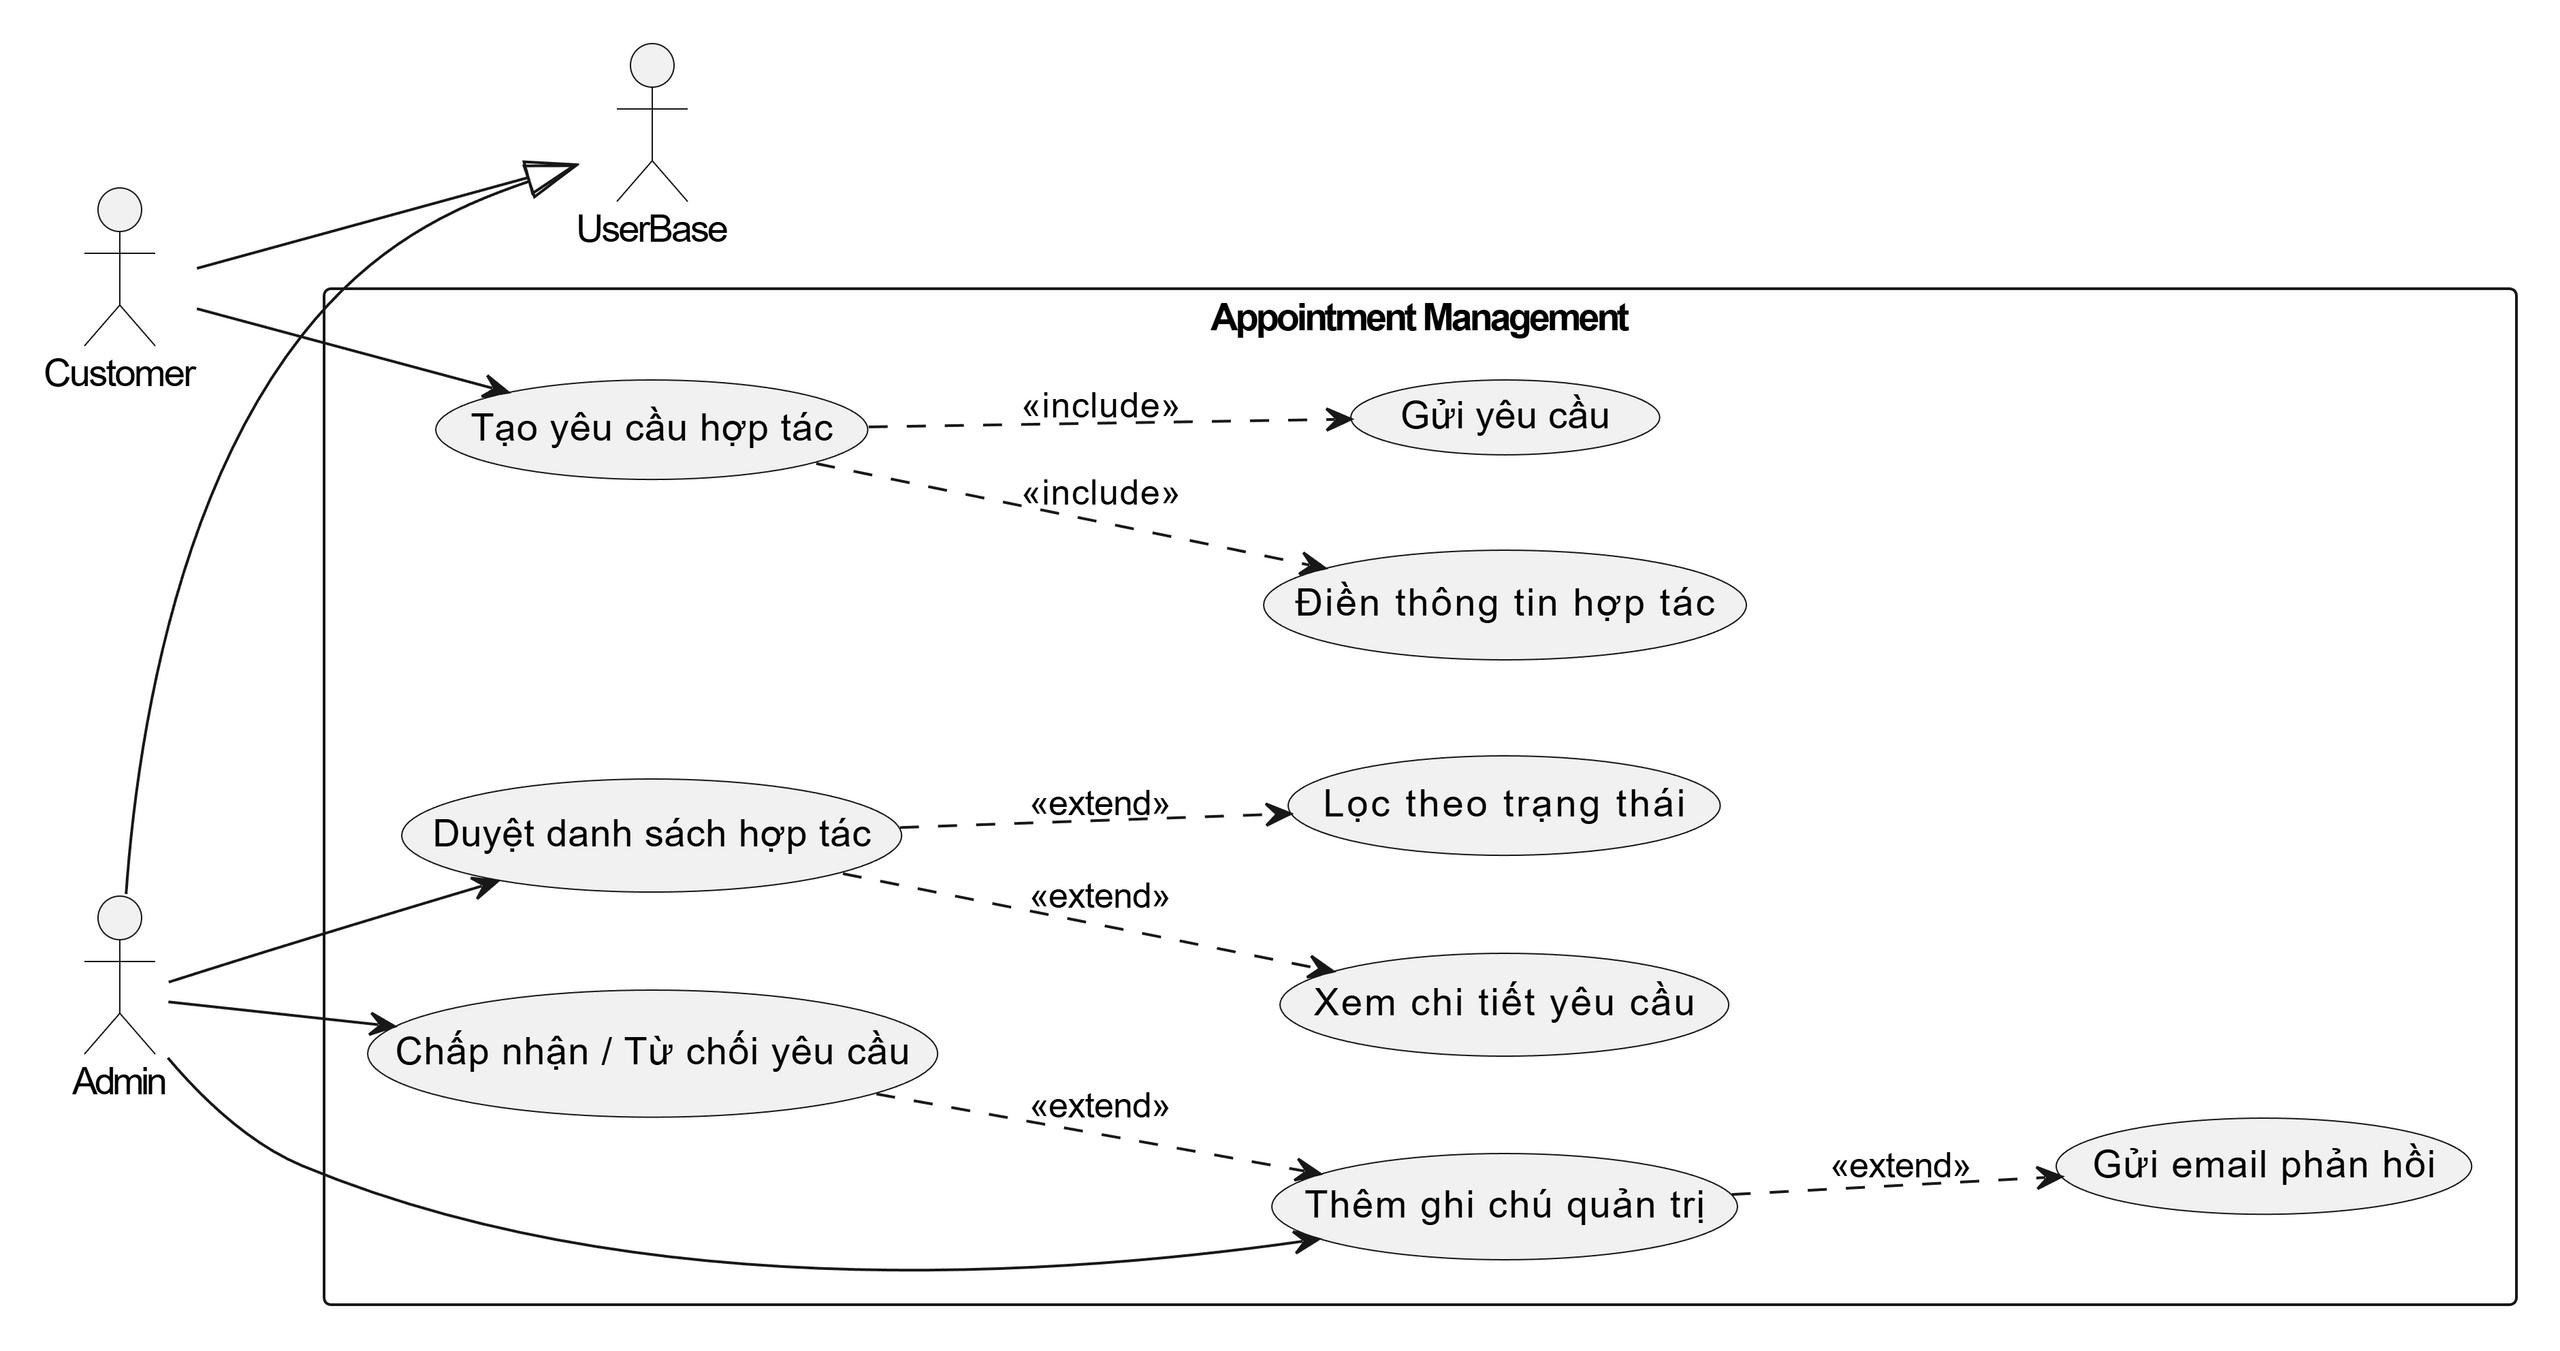
\includegraphics[width=1.0\textwidth]{figures/usecase_hoptac.jpg}
    \caption{Sơ đồ use case thợ cắt tóc và admin hợp tác}
    \label{fig:usecase_hoptac}
\end{figure}

Dưới đây là các đặc tả use case của thợ cắt tóc và admin hợp tác.

\begin{table}[H]
\centering
\caption{Đặc tả Use Case UC-19: Tạo yêu cầu hợp tác}
\label{tab:uc19}
\begin{tabular}{|p{4cm}|p{11cm}|}
\hline
\textbf{Actor} & Customer \\
\hline
\textbf{Mô tả} & Đăng ký chương trình đối tác / khách hàng thân thiết \\
\hline
\textbf{Luồng chính} & 
1. Include: Gửi yêu cầu hợp tác \newline
2. Include: Điền thông tin hợp tác \newline
3. Gửi yêu cầu đến hệ thống \\
\hline
\textbf{Hậu điều kiện} & Yêu cầu được ghi nhận \\
\hline
\end{tabular}
\end{table}


\begin{table}[H]
\centering
\caption{Đặc tả Use Case UC-20: Duyệt danh sách hợp tác}
\label{tab:uc20}
\begin{tabular}{|p{4cm}|p{11cm}|}
\hline
\textbf{Actor} & Admin \\
\hline
\textbf{Mô tả} & Xem và phê duyệt yêu cầu hợp tác \\
\hline
\textbf{Luồng chính} & 
1. Xem danh sách yêu cầu \newline
2. Extend: Lọc theo trạng thái \newline
3. Extend: Xem chi tiết yêu cầu \\
\hline
\textbf{Hậu điều kiện} & Không có \\
\hline
\end{tabular}
\end{table}


\begin{table}[H]
\centering
\caption{Đặc tả Use Case UC-21: Chấp nhận/Từ chối yêu cầu}
\label{tab:uc21}
\begin{tabular}{|p{4cm}|p{11cm}|}
\hline
\textbf{Actor} & Admin \\
\hline
\textbf{Mô tả} & Xử lý yêu cầu hợp tác \\
\hline
\textbf{Luồng chính} & 
1. Xem chi tiết yêu cầu \newline
2. Chấp nhận hoặc từ chối \newline
3. Extend: Thêm ghi chú quản trị \newline
4. Extend: Gửi email phản hồi \\
\hline
\textbf{Hậu điều kiện} & Trạng thái yêu cầu được cập nhật \\
\hline
\end{tabular}
\end{table}

%----------------------------------------------------------------Admin---------------
\begin{figure}[H]
    \centering
    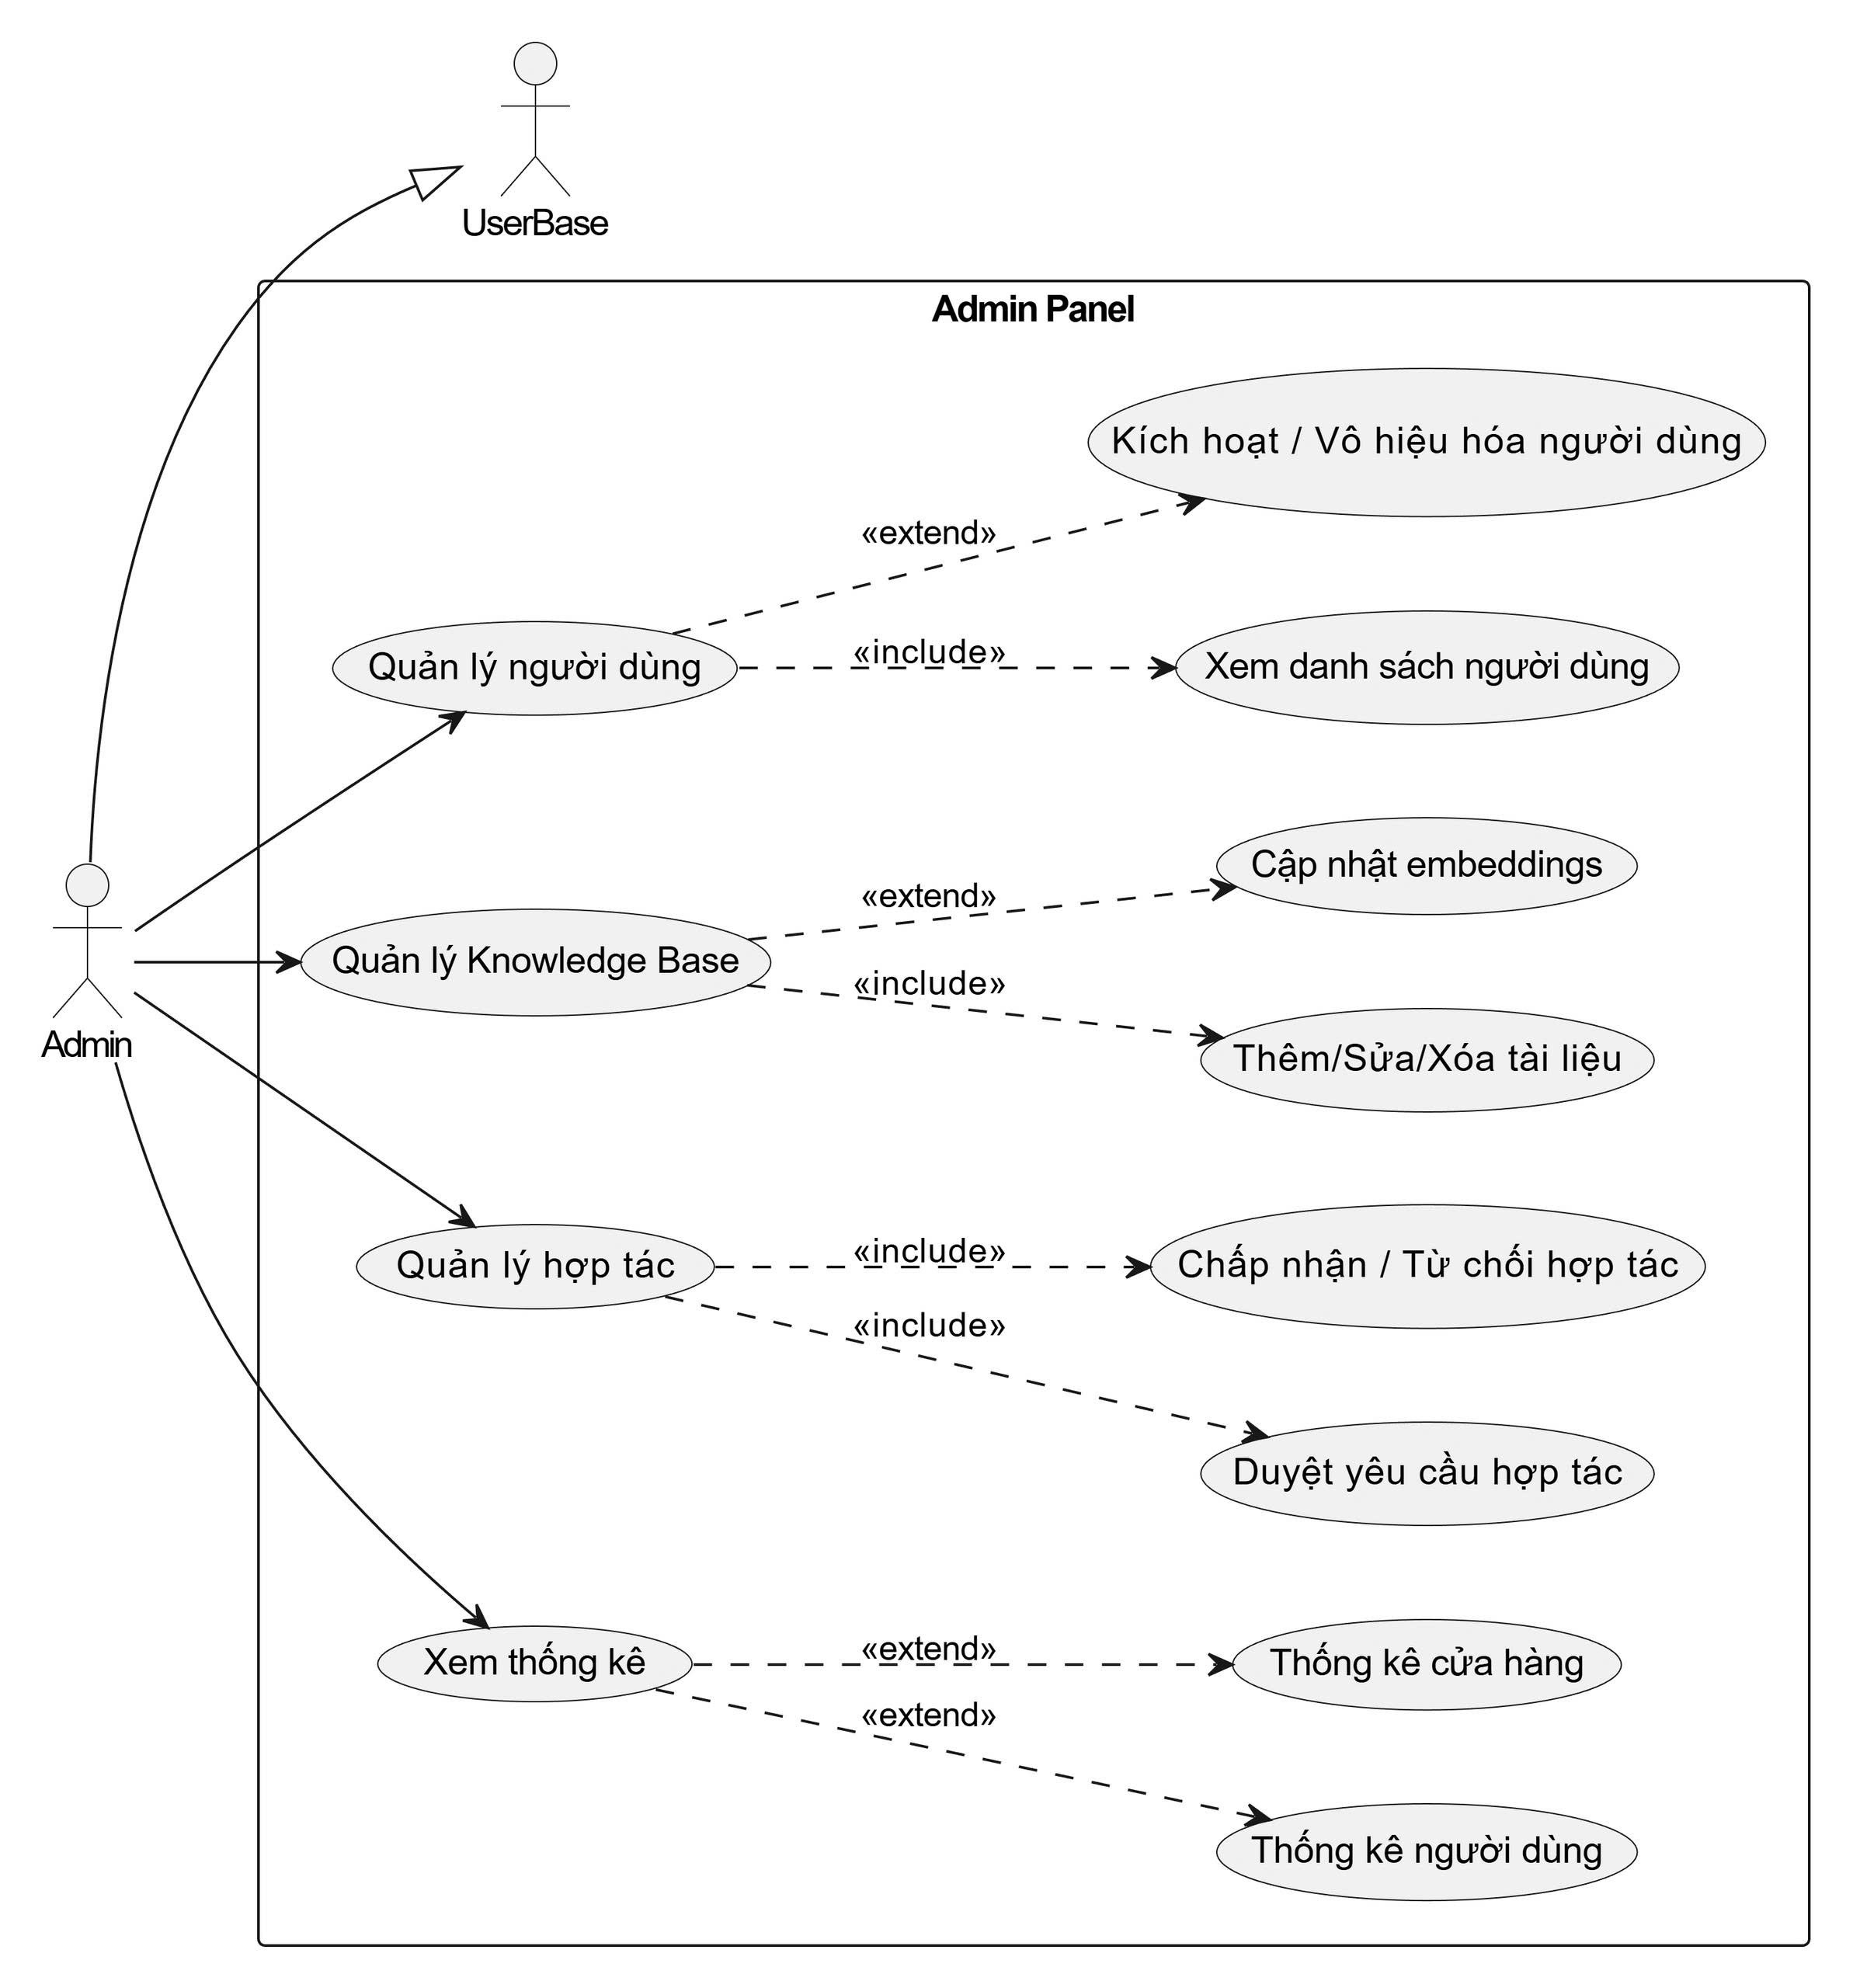
\includegraphics[width=1.0\textwidth]{figures/usecase_admin.jpg}
    \caption{Sơ đồ use case admin quản lý hệ thống}
    \label{fig:usecase_admin}
\end{figure}
Dưới đây là các đặc tả use case của admin quản lý hệ thống.

\begin{table}[H]
\centering
\caption{Đặc tả Use Case UC-22: Quản lý người dùng}
\label{tab:uc22}
\begin{tabular}{|p{4cm}|p{11cm}|}
\hline
\textbf{Actor} & Admin \\
\hline
\textbf{Mô tả} & Quản lý tài khoản người dùng \\
\hline
\textbf{Luồng chính} & 
1. Include: Xem danh sách người dùng \newline
2. Extend: Kích hoạt / Vô hiệu hóa người dùng \newline
3. Extend: Chỉnh sửa thông tin người dùng \\
\hline
\textbf{Hậu điều kiện} & Thông tin người dùng được cập nhật \\
\hline
\end{tabular}
\end{table}


\begin{table}[H]
\centering
\caption{Đặc tả Use Case UC-23: Xem thống kê}
\label{tab:uc23}
\begin{tabular}{|p{4cm}|p{11cm}|}
\hline
\textbf{Actor} & Admin \\
\hline
\textbf{Mô tả} & Xem báo cáo và thống kê hệ thống \\
\hline
\textbf{Luồng chính} & 
1. Chọn loại báo cáo \newline
2. Extend: Thống kê người dùng \newline
3. Extend: Thống kê đặt lịch \newline
4. Xuất báo cáo (PDF / Excel) \\
\hline
\textbf{Hậu điều kiện} & Không có \\
\hline
\end{tabular}
\end{table}


\begin{table}[H]
\centering
\caption{Đặc tả Use Case UC-24: Quản lý tất cả lịch hẹn}
\label{tab:uc24}
\begin{tabular}{|p{4cm}|p{11cm}|}
\hline
\textbf{Actor} & Admin \\
\hline
\textbf{Mô tả} & Giám sát và quản lý toàn bộ lịch hẹn trong hệ thống \\
\hline
\textbf{Luồng chính} & 
1. Include: Xem tất cả lịch hẹn \newline
2. Extend: Cập nhật trạng thái lịch hẹn \newline
3. Xử lý các vấn đề phát sinh \\
\hline
\textbf{Hậu điều kiện} & Lịch hẹn được quản lý \\
\hline
\end{tabular}
\end{table}



%---------------------------------------------------------------Thông báo---------------
\begin{figure}[H]
    \centering
    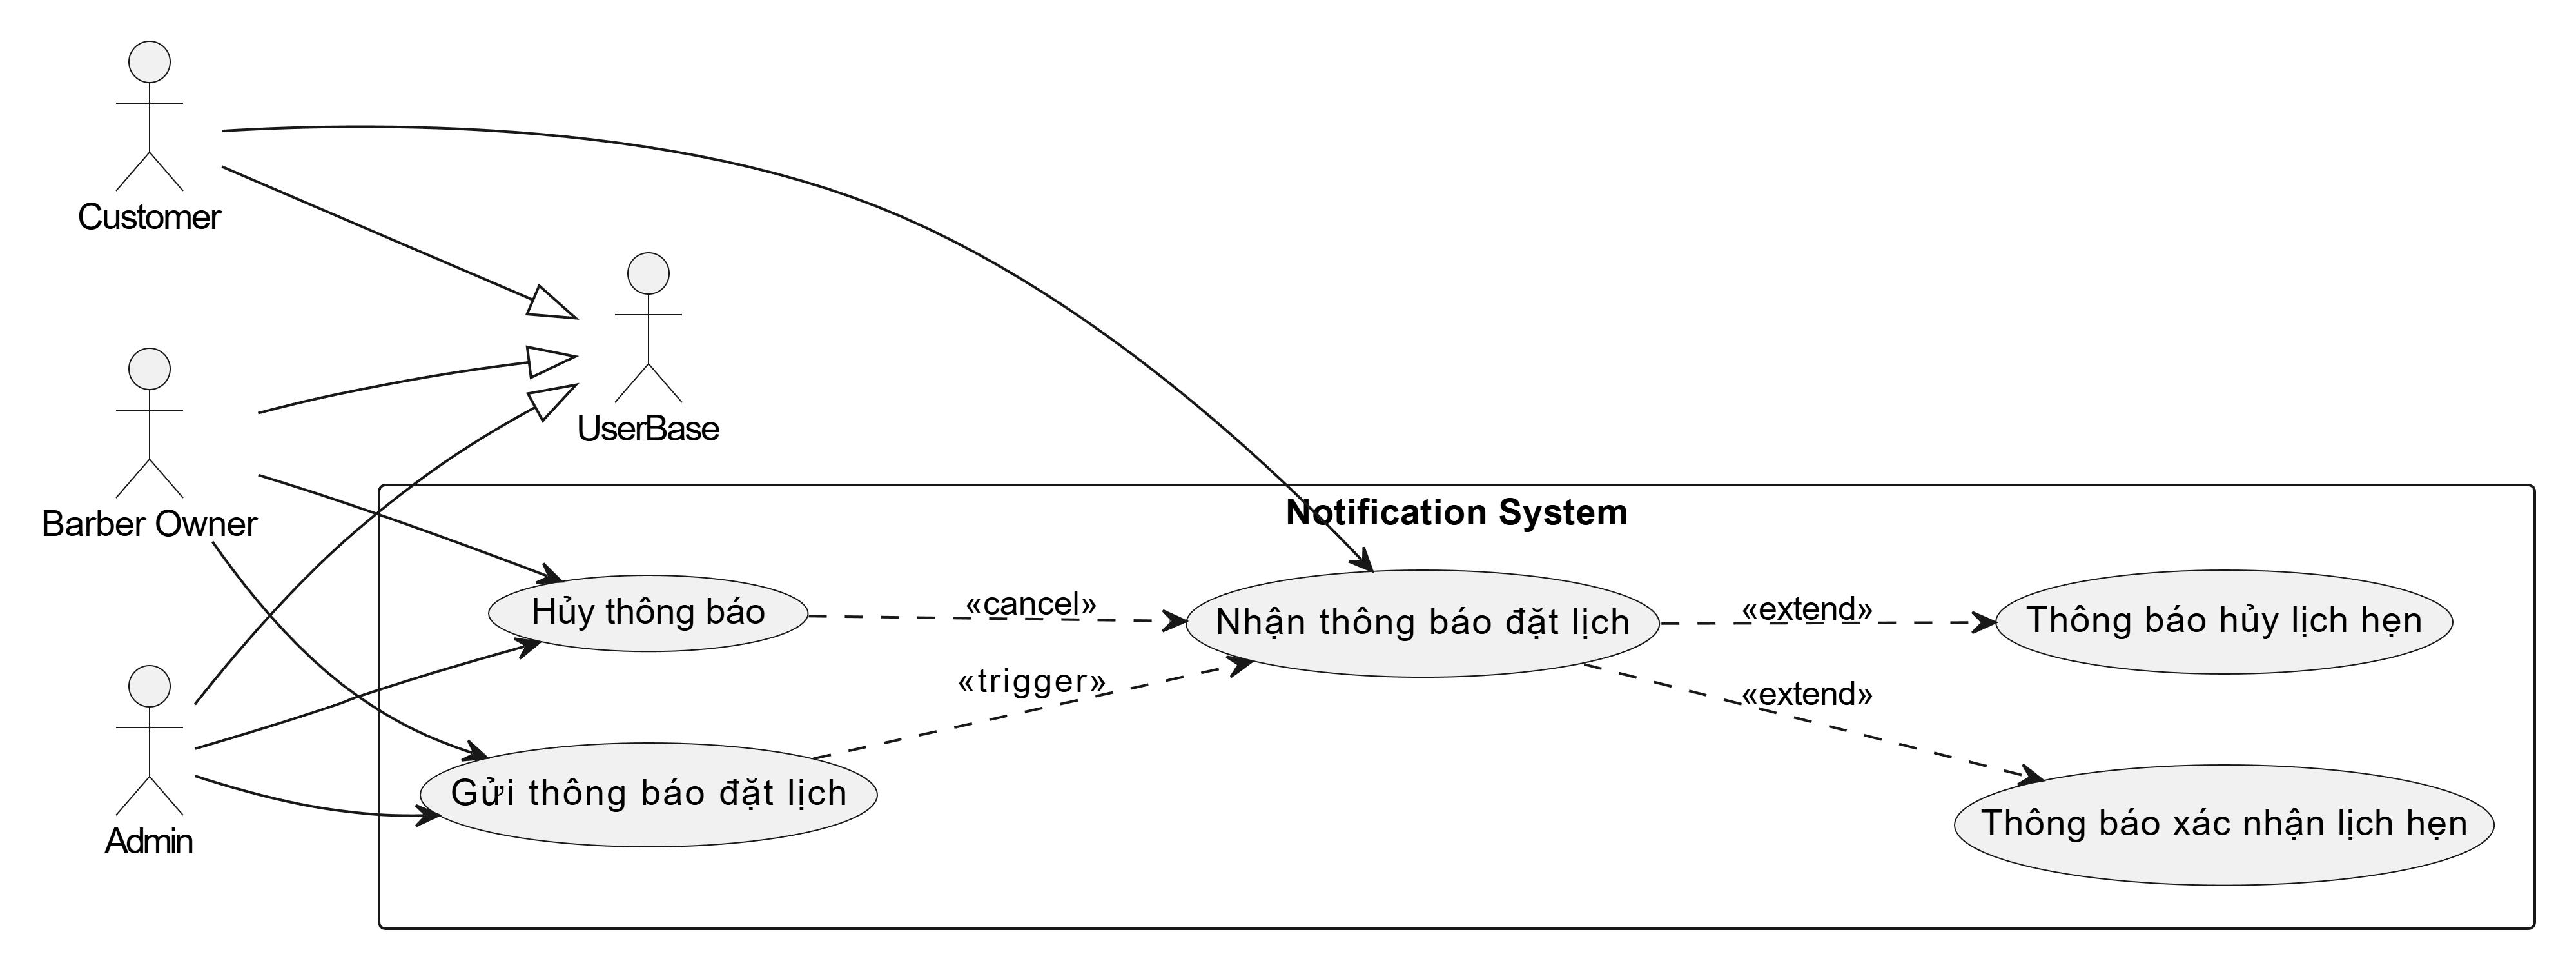
\includegraphics[width=1\textwidth]{figures/usecase_thongbao.jpg}
    \caption{Sơ đồ use case thông báo}
    \label{fig:usecase_thongbao}
\end{figure}
Dưới đây là các đặc tả use case của hệ thống thông báo.


\begin{table}[H]
\centering
\caption{Đặc tả Use Case UC-25: Hủy thông báo}
\label{tab:uc25}
\begin{tabular}{|p{4cm}|p{11cm}|}
\hline
\textbf{Actor} & Customer, Barber Owner, Admin \\
\hline
\textbf{Mô tả} & Xóa hoặc tắt các thông báo trong hệ thống \\
\hline
\textbf{Luồng chính} & 
1. Xem danh sách thông báo \newline
2. Extend: Tắt nhận thông báo đặt lịch \newline
3. Xóa thông báo đã đọc \\
\hline
\textbf{Hậu điều kiện} & Thông báo được xóa hoặc bị vô hiệu hóa \\
\hline
\end{tabular}
\end{table}


\begin{table}[H]
\centering
\caption{Đặc tả Use Case UC-26: Gửi thông báo đặt lịch}
\label{tab:uc26}
\begin{tabular}{|p{4cm}|p{11cm}|}
\hline
\textbf{Actor} & Hệ thống (tự động) \\
\hline
\textbf{Mô tả} & Gửi thông báo tự động khi có sự kiện liên quan đến lịch hẹn \\
\hline
\textbf{Luồng chính} & 
1. Trigger: Khi có sự kiện đặt lịch hoặc thay đổi lịch \newline
2. Tạo nội dung thông báo \newline
3. Extend: Thông báo hủy lịch hẹn \newline
4. Extend: Thông báo xác nhận lịch hẹn \newline
5. Gửi thông báo qua Push Notification / Email / SMS \\
\hline
\textbf{Hậu điều kiện} & Thông báo được gửi đến người dùng \\
\hline
\end{tabular}
\end{table}


\begin{table}[H]
\centering
\caption{Đặc tả Use Case UC-27: Nhận thông báo đặt lịch}
\label{tab:uc27}
\begin{tabular}{|p{4cm}|p{11cm}|}
\hline
\textbf{Actor} & Customer, Barber Owner \\
\hline
\textbf{Mô tả} & Nhận và xem thông báo liên quan đến lịch hẹn \\
\hline
\textbf{Luồng chính} & 
1. Nhận thông báo trên thiết bị \newline
2. Đọc nội dung thông báo \newline
3. Mở ứng dụng để xem chi tiết lịch hẹn \\
\hline
\textbf{Hậu điều kiện} & Thông báo được đánh dấu là đã đọc \\
\hline
\end{tabular}
\end{table}

\section{Activity Diagram}
\subsection{Activity Diagram xử lý đăng ký}
\begin{figure}[H]
    \centering
    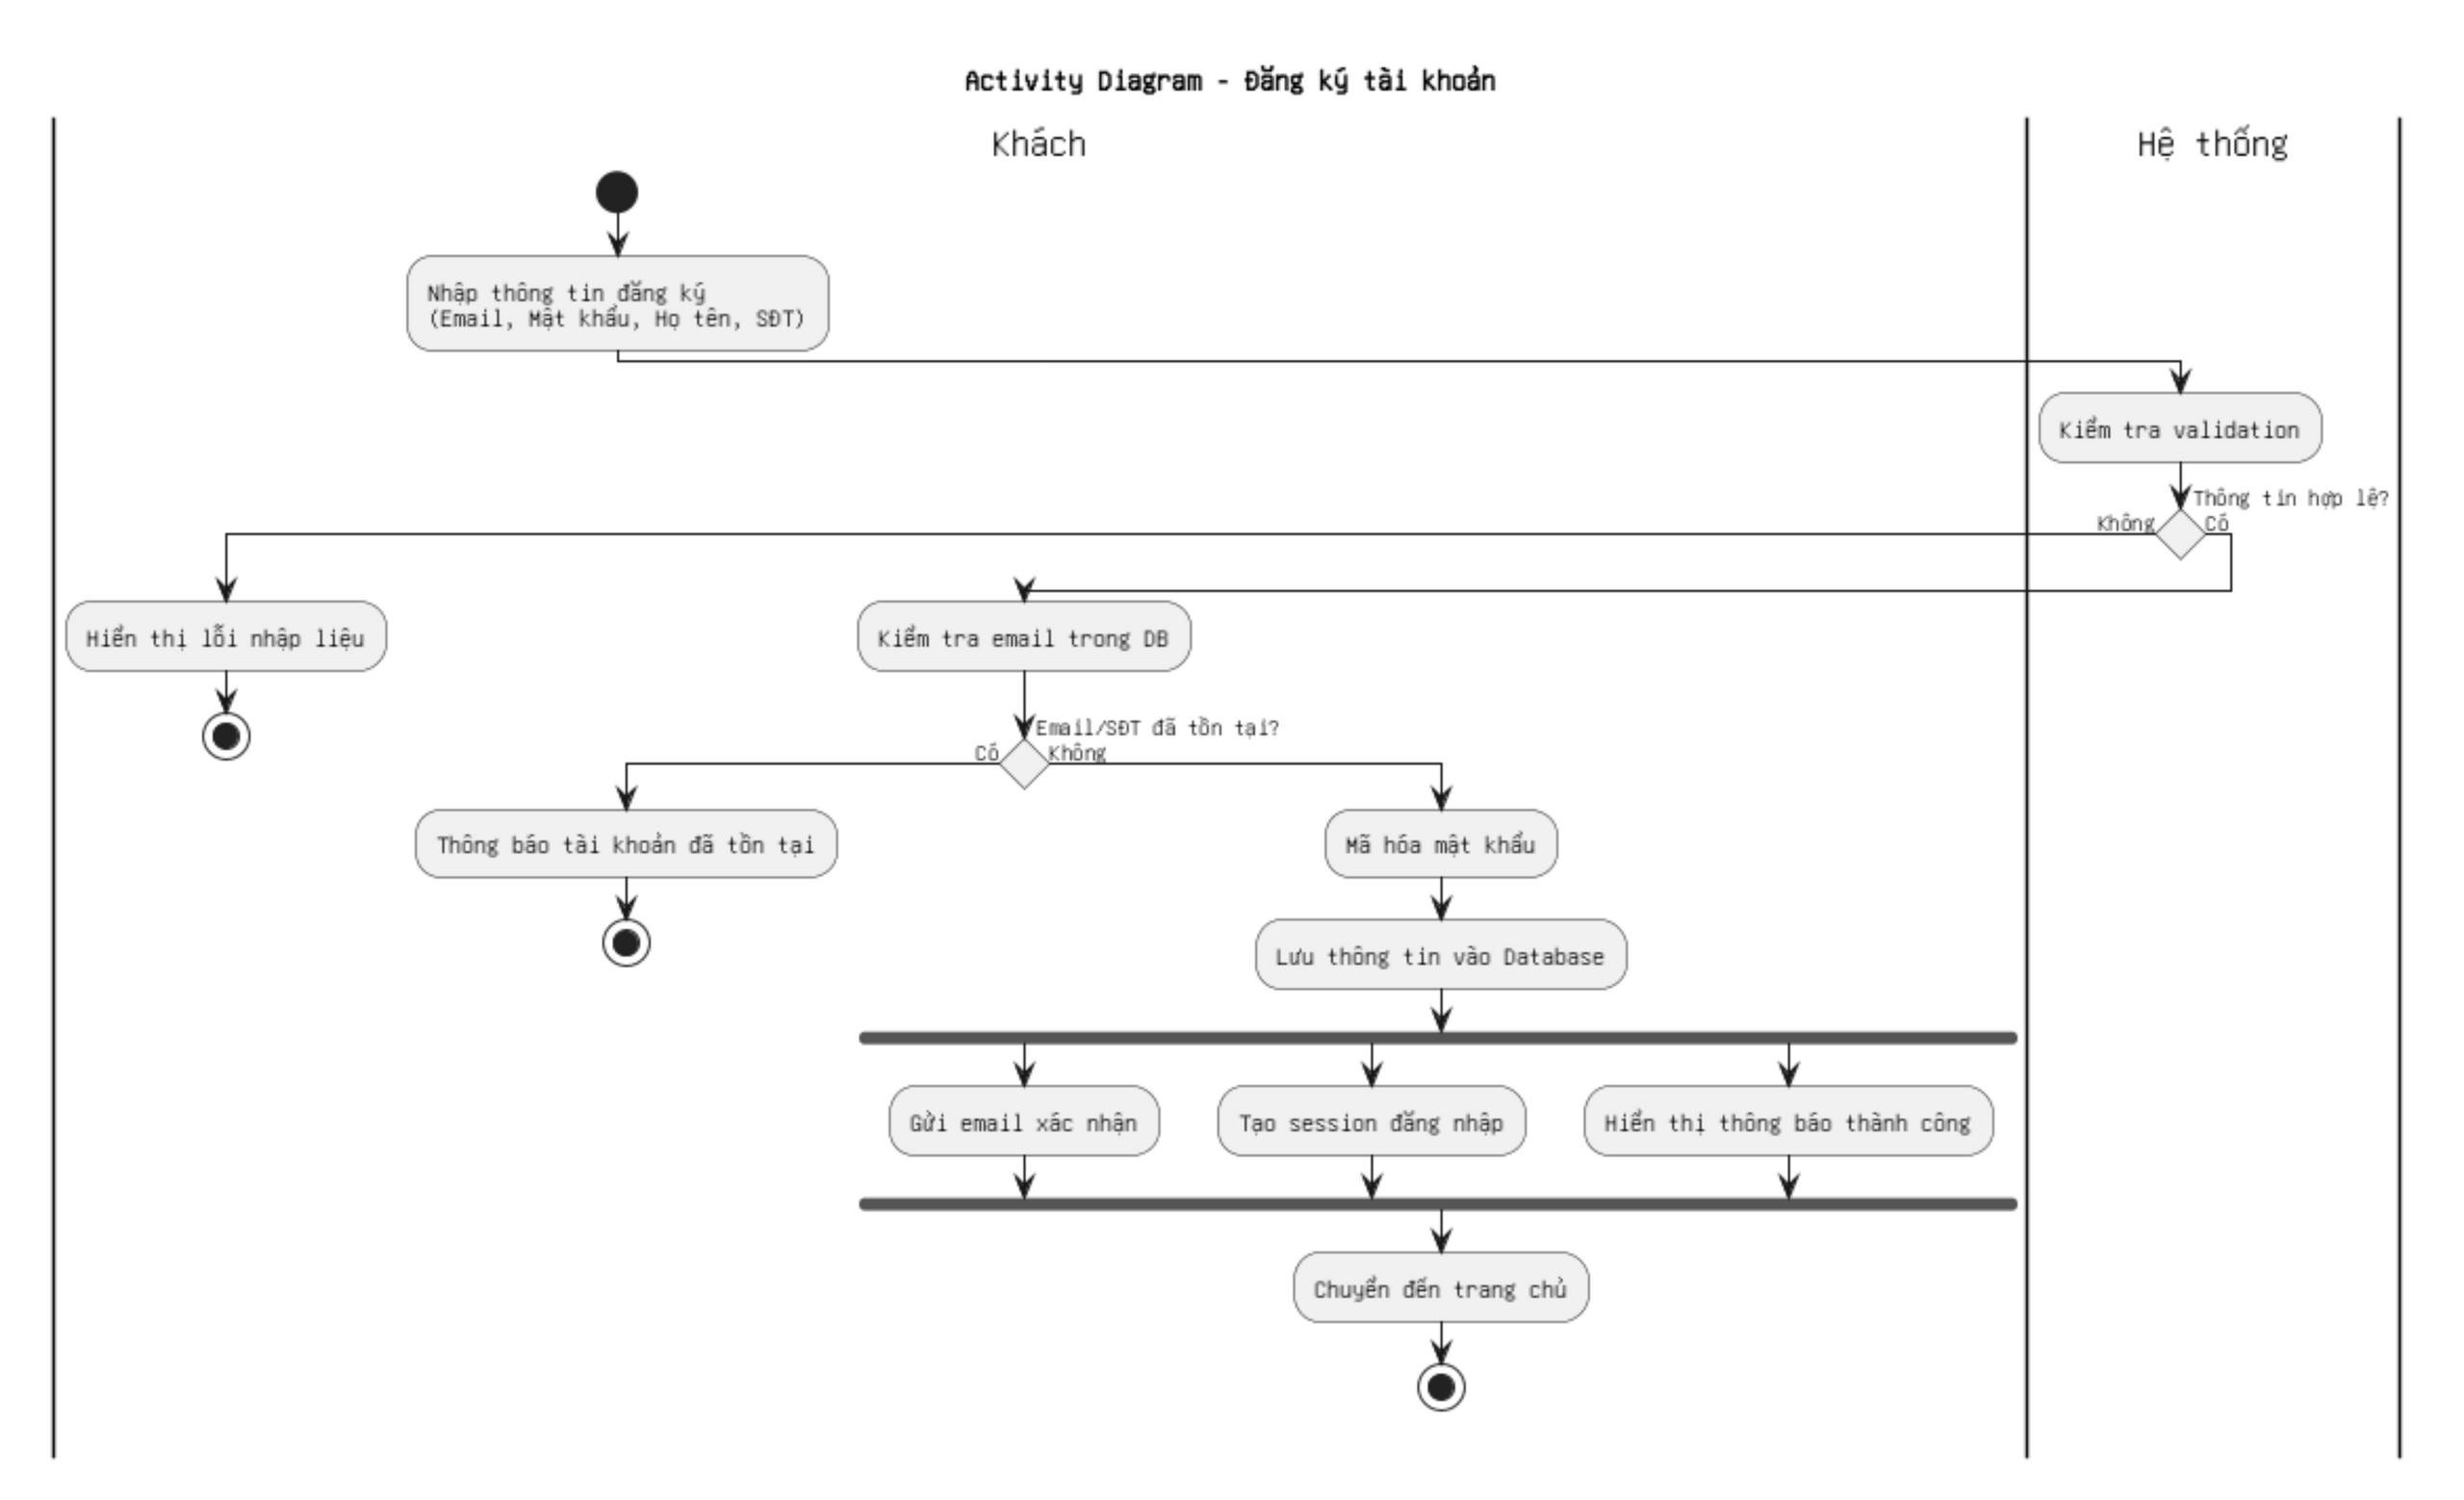
\includegraphics[width=0.7\textwidth]{figures/ac_dk.jpg}
    \caption{Activity Diagram xử lý đăng ký}
    \label{fig:ac_dk}
\end{figure}

\textbf{Mục đích:} Cho phép người dùng tạo tài khoản mới trong hệ thống bằng cách nhập thông tin cá nhân và xác thực qua email.

\textbf{Luồng hoạt động:}

\begin{itemize}
    \item Khách hàng nhập thông tin đăng ký (Email, Mật khẩu, Họ tên).
    \item Hệ thống kiểm tra validation thông tin:
    \begin{itemize}
        \item \textit{Nếu không hợp lệ:} Hiển thị lỗi nhập liệu và kết thúc.
        \item \textit{Nếu hợp lệ:} Tiếp tục kiểm tra email trong database.
    \end{itemize}
    \item Hệ thống kiểm tra email đã tồn tại:
    \begin{itemize}
        \item \textit{Nếu đã tồn tại:} Thông báo tài khoản đã tồn tại và kết thúc.
        \item \textit{Nếu chưa tồn tại:} Mã hóa mật khẩu và lưu thông tin vào database.
    \end{itemize}
    \item Hệ thống thực hiện song song:
    \begin{itemize}
        \item Gửi email xác nhận
        \item Tạo session đăng nhập
        \item Hiển thị thông báo thành công
    \end{itemize}
    \item Chuyển đến trang chủ và kết thúc quy trình.
\end{itemize}



\subsection{Activity Diagram xử lý đăng nhập}
\begin{figure}[H]
    \centering
    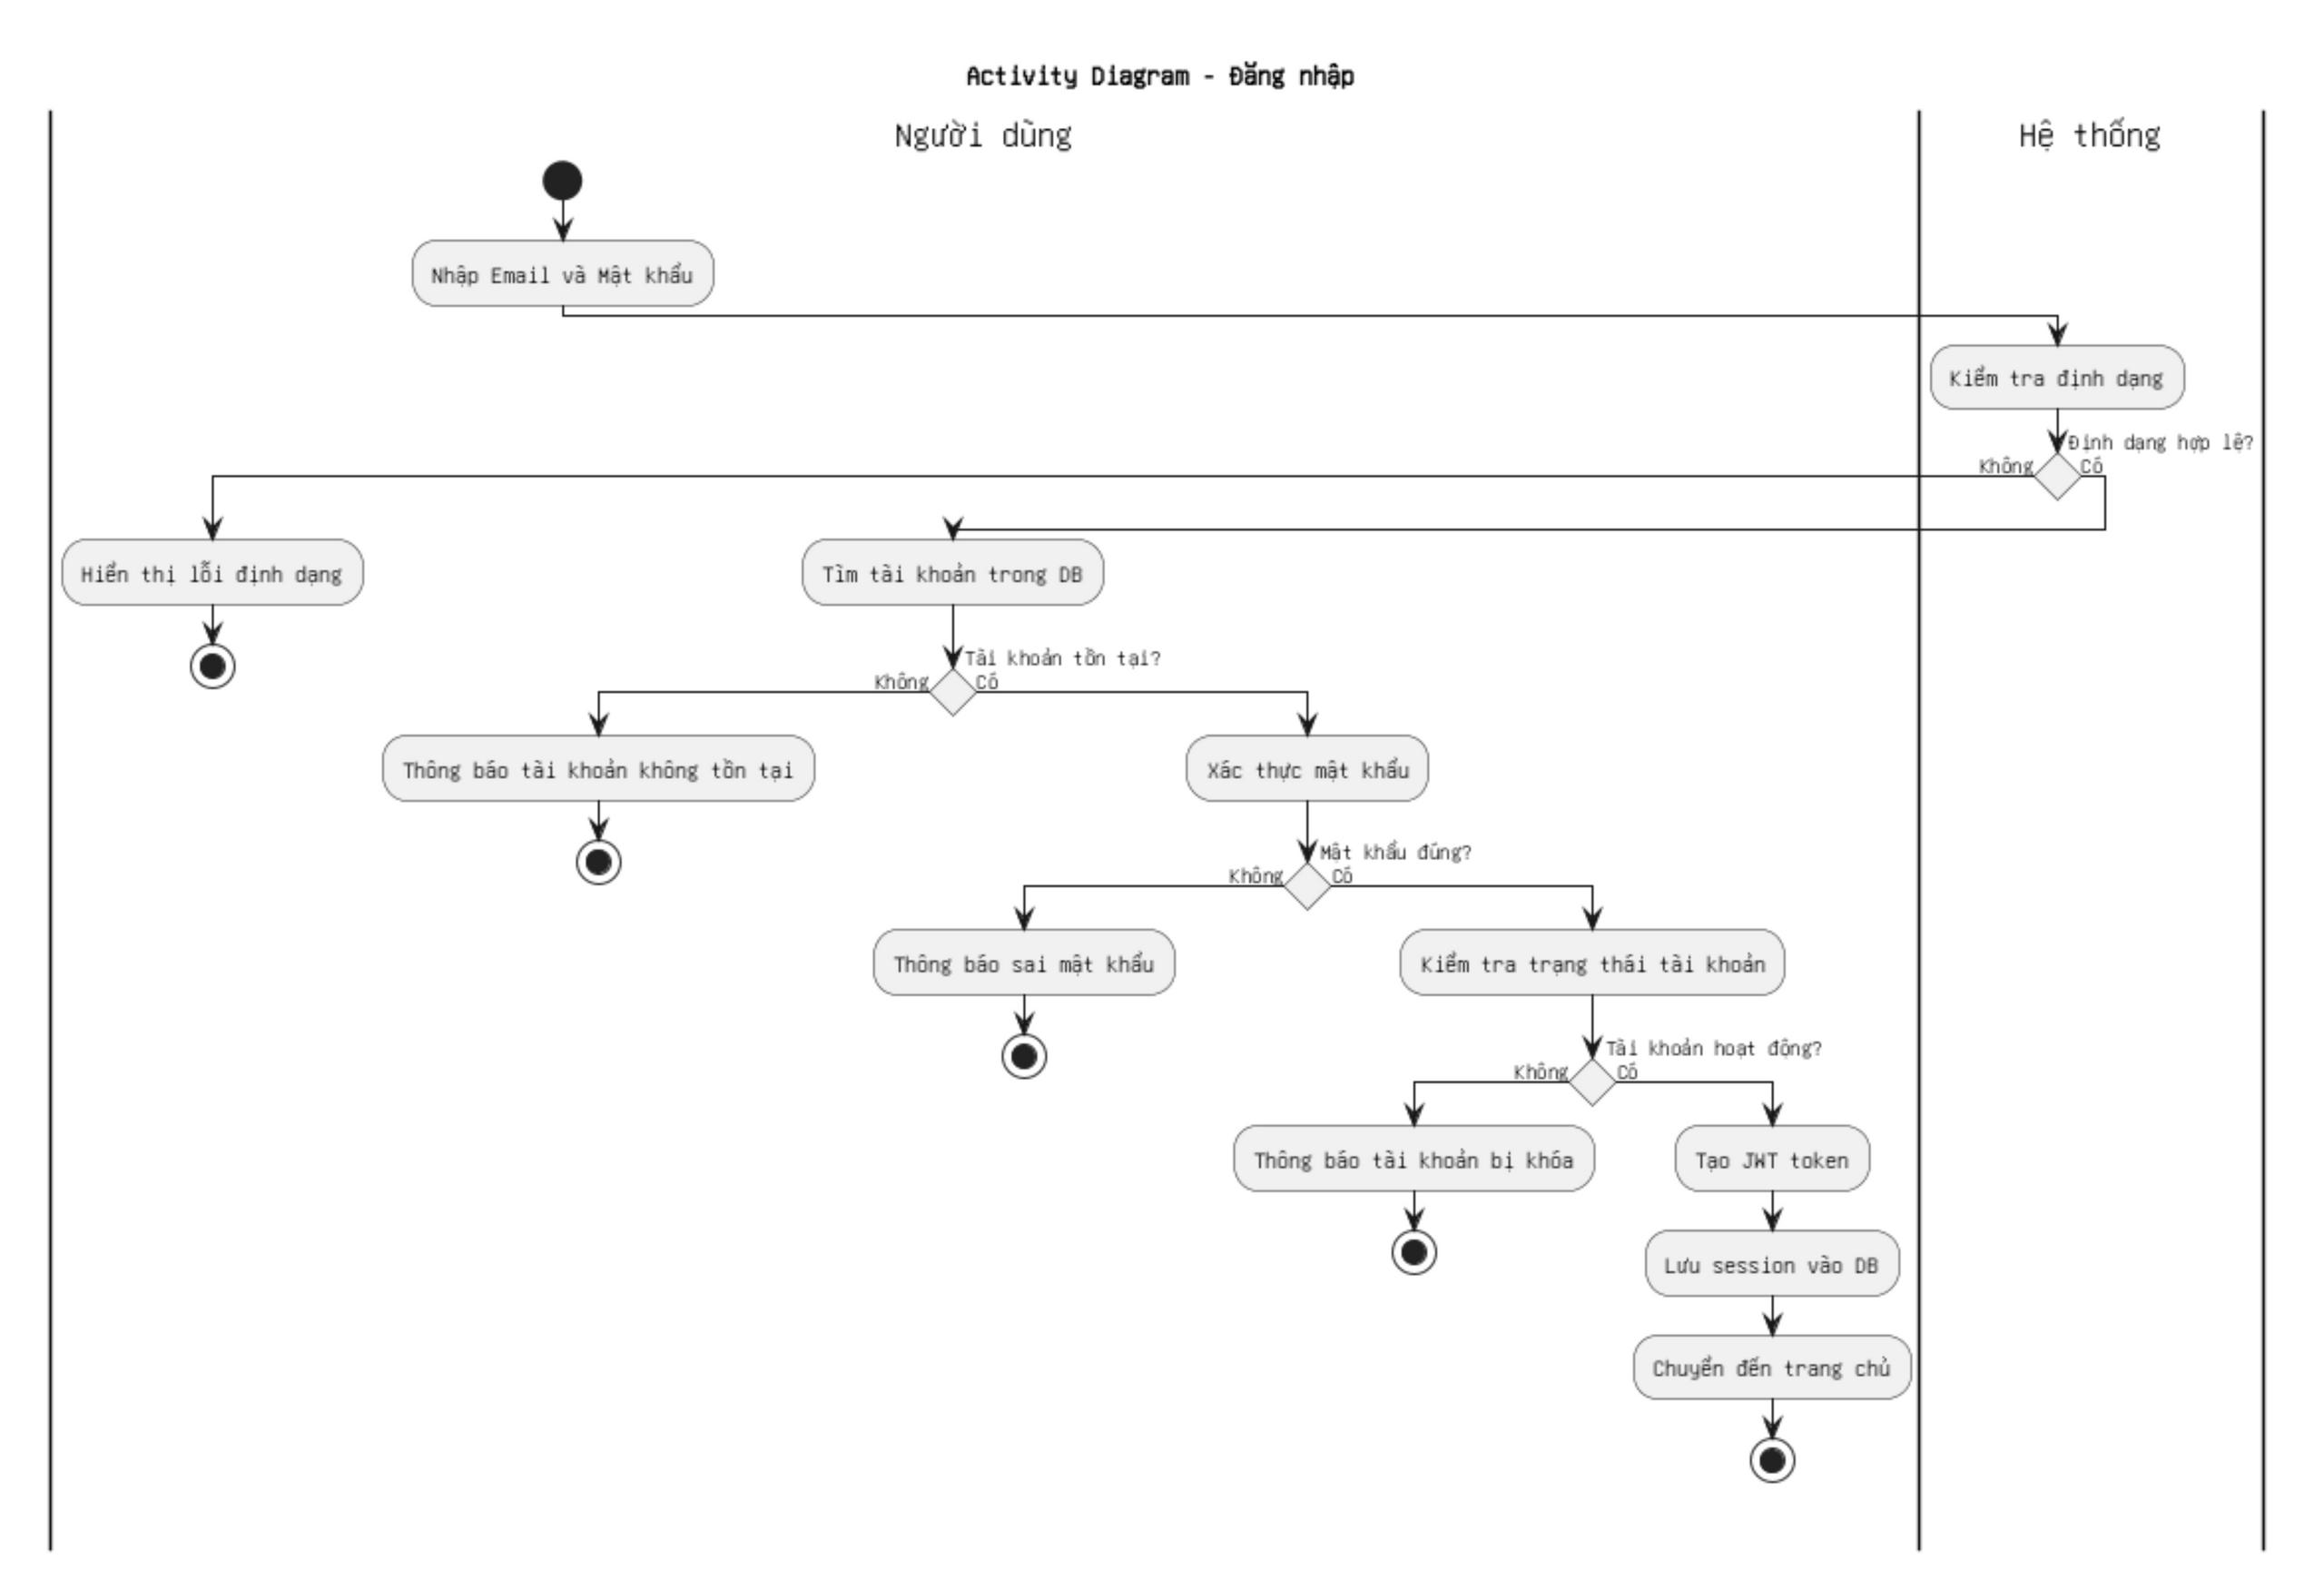
\includegraphics[width=0.7\textwidth]{figures/ac_dn.jpg}
    \caption{Activity Diagram xử lý đăng nhập}
    \label{fig:ac_dn}
\end{figure}
\textbf{Mục đích:} Cho phép người dùng xác thực và truy cập vào hệ thống bằng tài khoản đã đăng ký.

\textbf{Luồng hoạt động:}

\begin{itemize}
    \item Người dùng nhập Email và Mật khẩu.
    \item Hệ thống kiểm tra định dạng:
    \begin{itemize}
        \item \textit{Nếu không hợp lệ:} Hiển thị lỗi định dạng và kết thúc.
        \item \textit{Nếu hợp lệ:} Tìm tài khoản trong database.
    \end{itemize}
    \item Hệ thống kiểm tra tài khoản tồn tại:
    \begin{itemize}
        \item \textit{Nếu không tồn tại:} Thông báo tài khoản không tồn tại và kết thúc.
        \item \textit{Nếu tồn tại:} Xác thực mật khẩu.
    \end{itemize}
    \item Hệ thống xác thực mật khẩu:
    \begin{itemize}
        \item \textit{Nếu sai:} Thông báo sai mật khẩu và kết thúc.
        \item \textit{Nếu đúng:} Kiểm tra trạng thái tài khoản.
    \end{itemize}
    \item Hệ thống kiểm tra tài khoản hoạt động:
    \begin{itemize}
        \item \textit{Nếu bị khóa:} Thông báo tài khoản bị khóa và kết thúc.
        \item \textit{Nếu hoạt động:} Tạo JWT token.
    \end{itemize}
    \item Lưu session vào database.
    \item Chuyển đến trang chủ và kết thúc quy trình.
\end{itemize}




\subsection{Activity Diagram xử lý đặt lịch}
\begin{figure}[H]
    \centering
    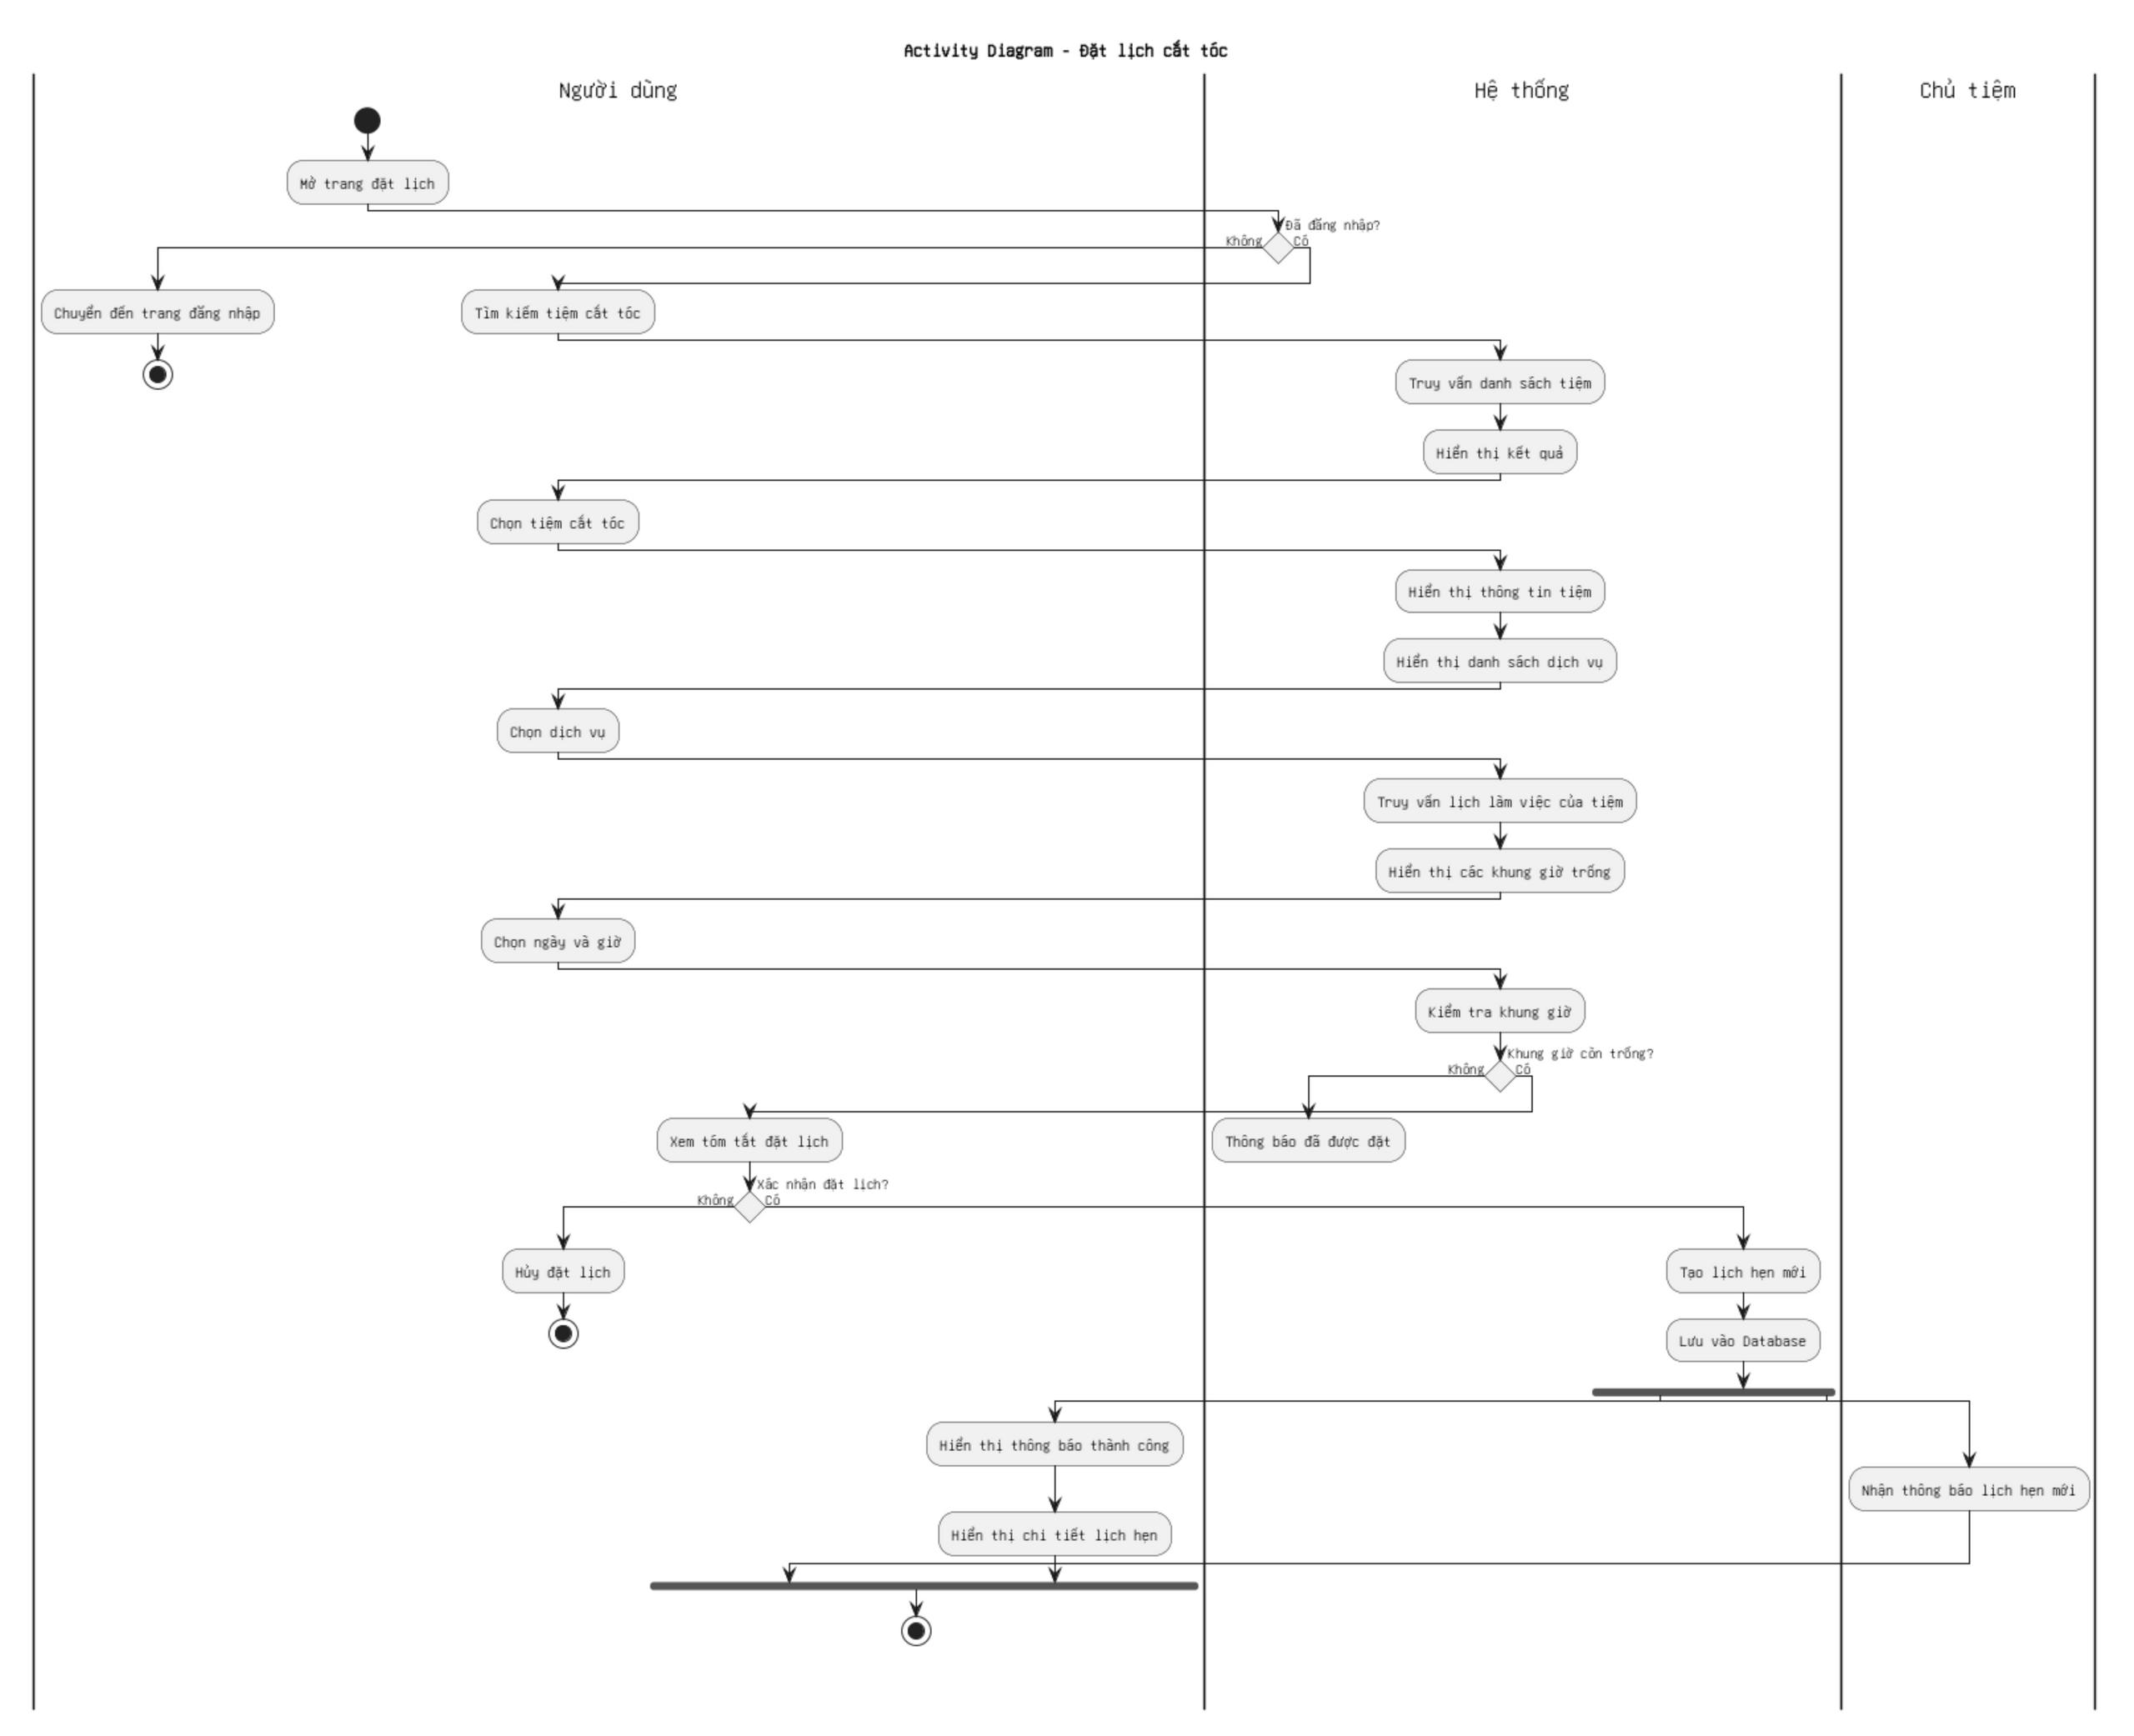
\includegraphics[width=0.7\textwidth]{figures/ac_booking.jpg}
    \caption{Activity Diagram xử lý đặt lịch}
    \label{fig:ac_booking}
\end{figure}

\textbf{Mục đích:} Cho phép người dùng đặt lịch hẹn cắt tóc tại tiệm bằng cách chọn thông tin liên quan và xác nhận đặt lịch.

\textbf{Luồng hoạt động:}

\begin{itemize}
    \item Người dùng mở trang đặt lịch.
    \item Hệ thống kiểm tra đăng nhập:
    \begin{itemize}
        \item \textit{Nếu chưa đăng nhập:} Chuyển đến trang đăng nhập và kết thúc.
        \item \textit{Nếu đã đăng nhập:} Tìm kiếm liên cắt tóc.
    \end{itemize}
    \item Chủ tiệm truy vấn danh sách tiệm và hiển thị kết quả.
    \item Người dùng chọn liệm cắt tóc, hệ thống hiển thị thông tin tiệm và kiểm tra danh sách dịch vụ.
    \item Người dùng chọn dịch vụ, hệ thống truy vấn liên lịch làm việc của tiệm và hiển thị các khung giờ trống.
    \item Người dùng chọn ngày và giờ, hệ thống kiểm tra khung giờ:
    \begin{itemize}
        \item \textit{Nếu khung giờ còn trống:} Thông báo đã được đặt.
        \item \textit{Nếu khung giờ đã hết:} Chờ người dùng chọn lại.
    \end{itemize}
    \item Người dùng xem tóm tắt đặt lịch và xác nhận đặt lịch:
    \begin{itemize}
        \item \textit{Nếu có nhận đặt lịch:} Hủy đặt lịch và kết thúc.
        \item \textit{Nếu xác nhận:} 
        \begin{itemize}
            \item Chủ tiệm tạo lịch hẹn mới và lưu vào database.
            \item Gửi thông báo lịch hẹn mới.
        \end{itemize}
    \end{itemize}
    \item Hiển thị thông báo thành công và chi tiết lịch hẹn.
    \item Kết thúc quy trình.
\end{itemize}


\subsection{Activity Diagram xử lý AI gợi ý kiểu tóc}
\begin{figure}[H]
    \centering
    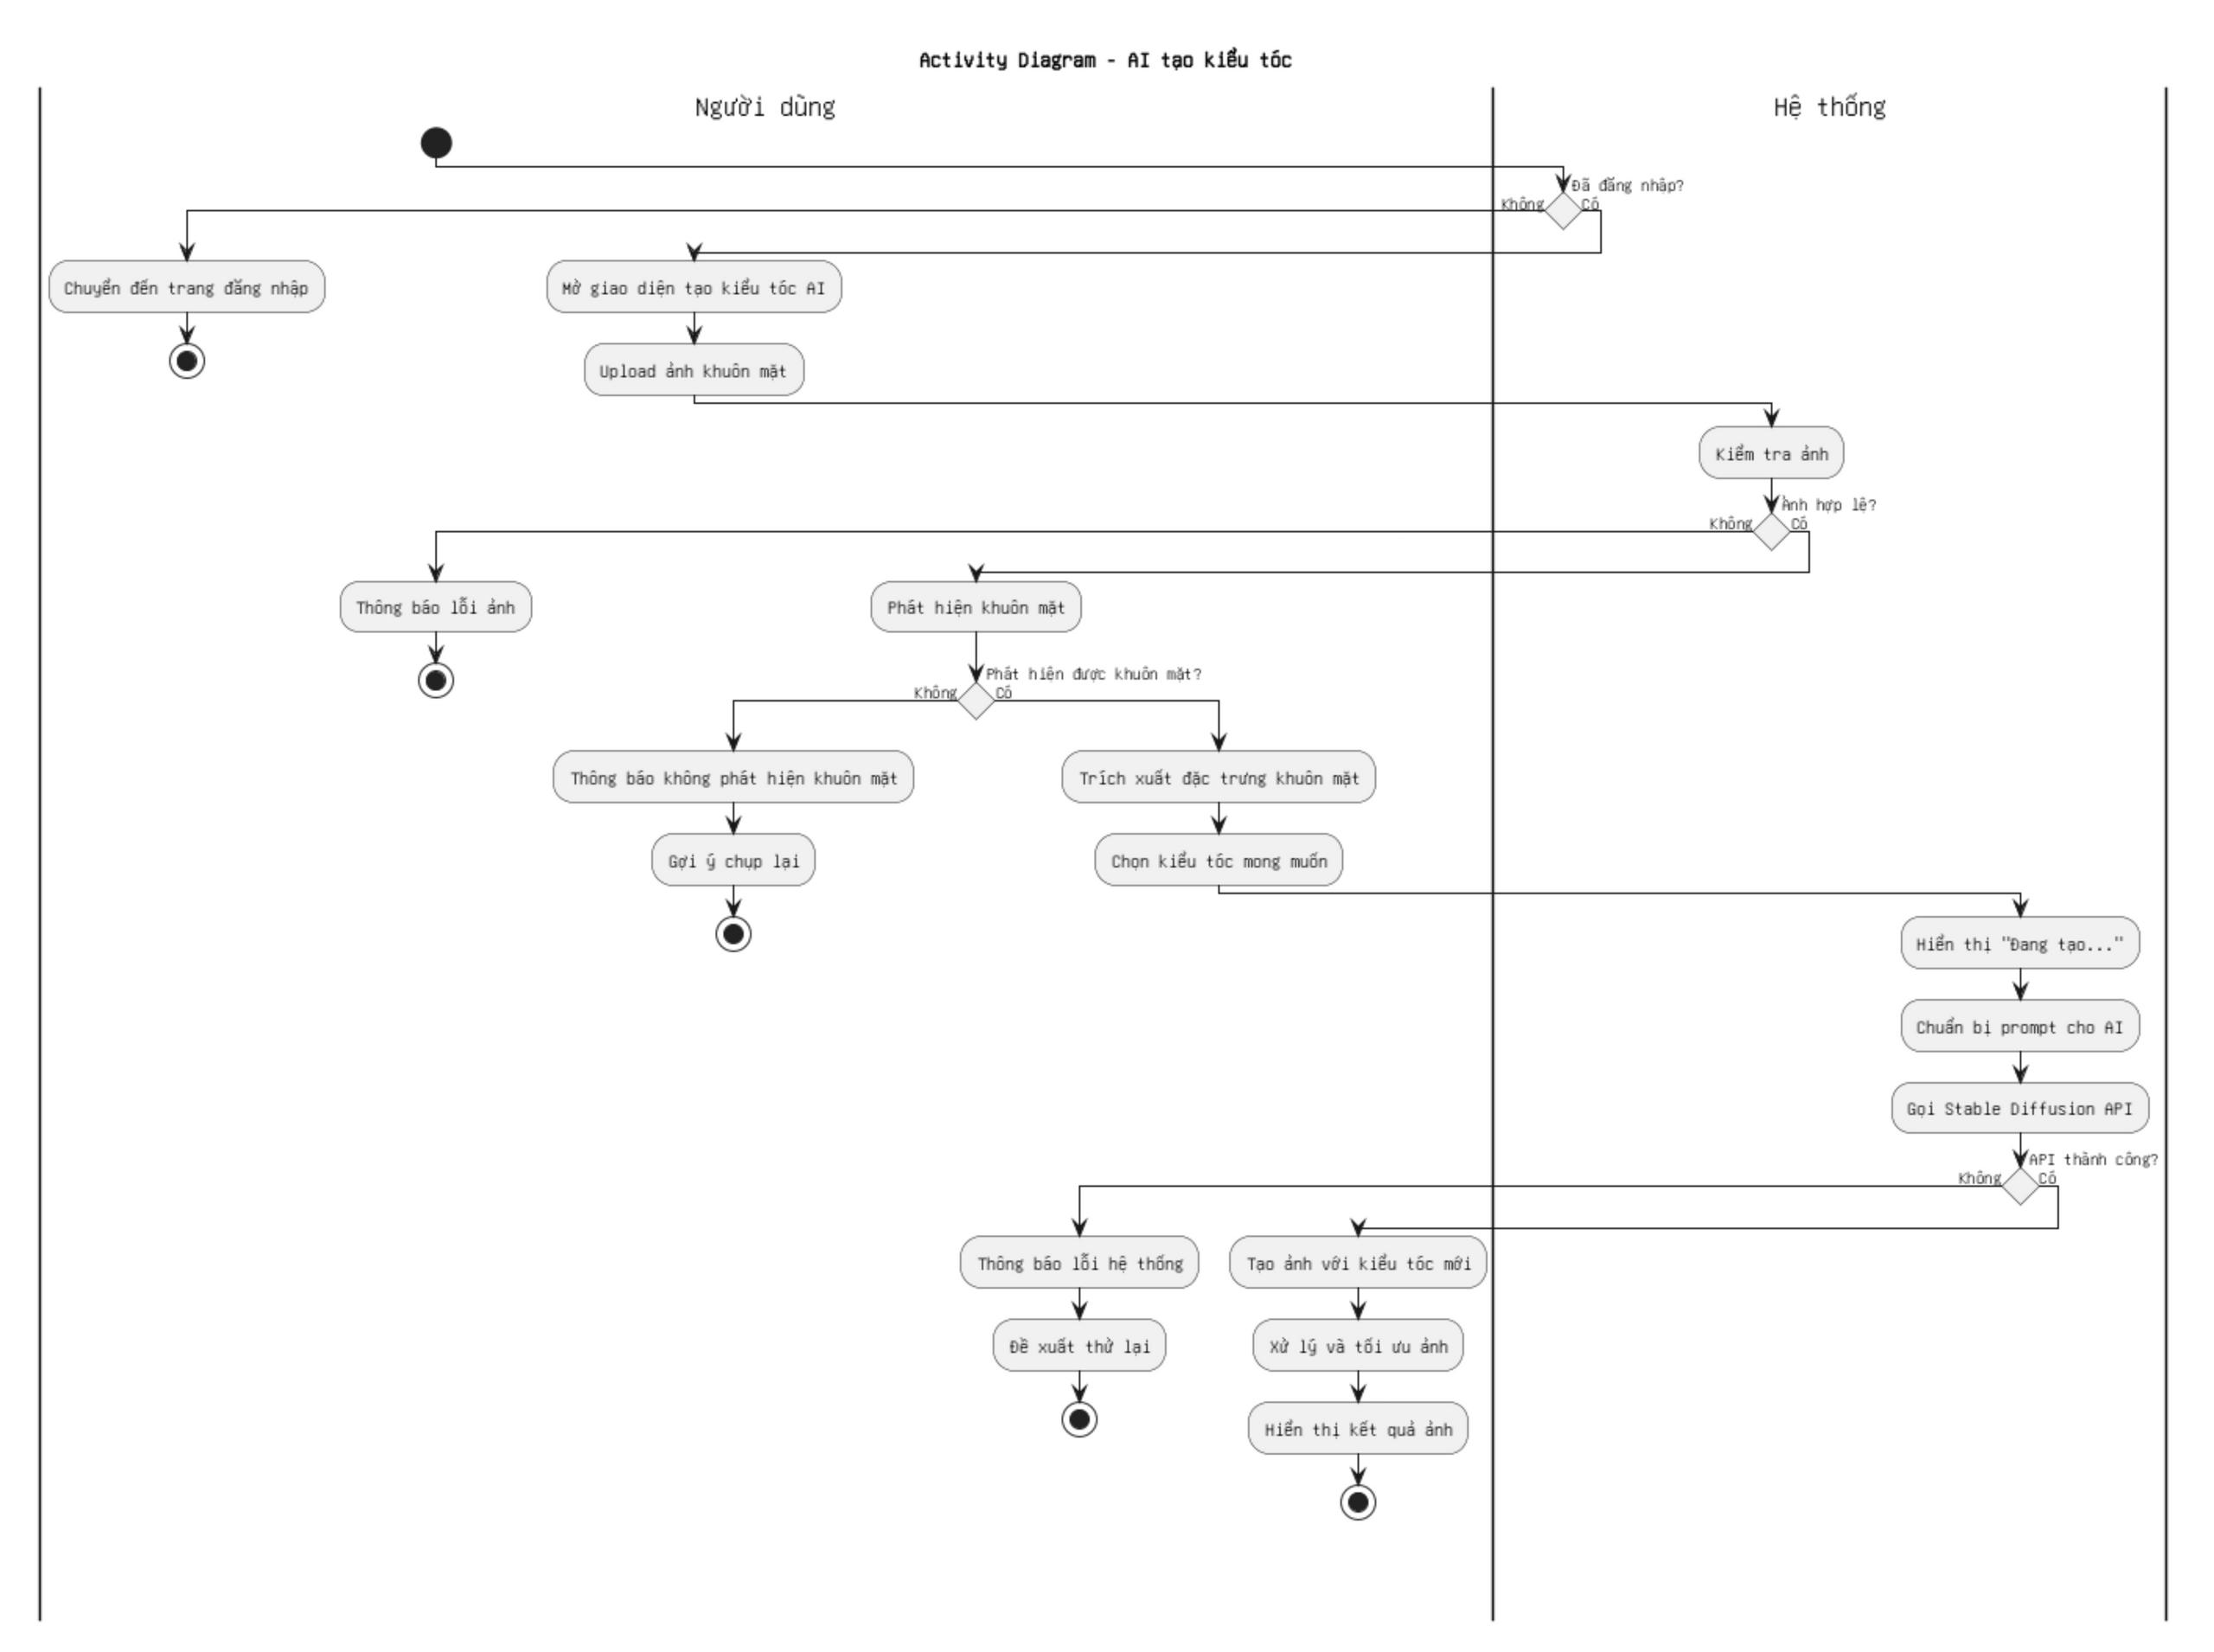
\includegraphics[width=0.8\textwidth]{figures/ac_hair.jpg}
    \caption{Activity Diagram xử lý AI gợi ý kiểu tóc}
    \label{fig:ac_hair}
\end{figure}

\textbf{Mục đích:} Cho phép người dùng sử dụng AI để tạo và xem trước kiểu tóc mong muốn từ ảnh khuôn mặt.

\textbf{Luồng hoạt động:}

\begin{itemize}
    \item Hệ thống kiểm tra đăng nhập:
    \begin{itemize}
        \item \textit{Nếu chưa đăng nhập:} Chuyển đến trang đăng nhập và kết thúc.
        \item \textit{Nếu đã đăng nhập:} Mở giao diện tạo kiểu tóc AI.
    \end{itemize}
    \item Người dùng upload ảnh khuôn mặt.
    \item Hệ thống kiểm tra định dạng ảnh:
    \begin{itemize}
        \item \textit{Nếu không hợp lệ:} Thông báo lỗi ảnh và kết thúc.
        \item \textit{Nếu hợp lệ:} Phát hiện khuôn mặt.
    \end{itemize}
    \item Hệ thống phát hiện được khuôn mặt:
    \begin{itemize}
        \item \textit{Nếu không:} Thông báo không phát hiện khuôn mặt, gửi ý chụp lại và kết thúc.
        \item \textit{Nếu có:} Trích xuất đặc trưng khuôn mặt và chọn kiểu tóc mong muốn.
    \end{itemize}
    \item Hệ thống:
    \begin{itemize}
        \item Hiển thị "Đang tạo..."
        \item Chuẩn bị prompt cho AI
        \item Gọi Stable Diffusion API
    \end{itemize}
    \item Kiểm tra API thành công:
    \begin{itemize}
        \item \textit{Nếu không:} Thông báo lỗi hệ thống, đề xuất thử lại và kết thúc.
        \item \textit{Nếu có:} Tạo ảnh với kiểu tóc mới, xử lý và tối ưu ảnh, hiển thị kết quả ảnh.
    \end{itemize}
    \item Kết thúc quy trình.
\end{itemize}

\subsection{Activity Diagram xử lý AI kiểm tra da mặt}
\begin{figure}[H]
    \centering
    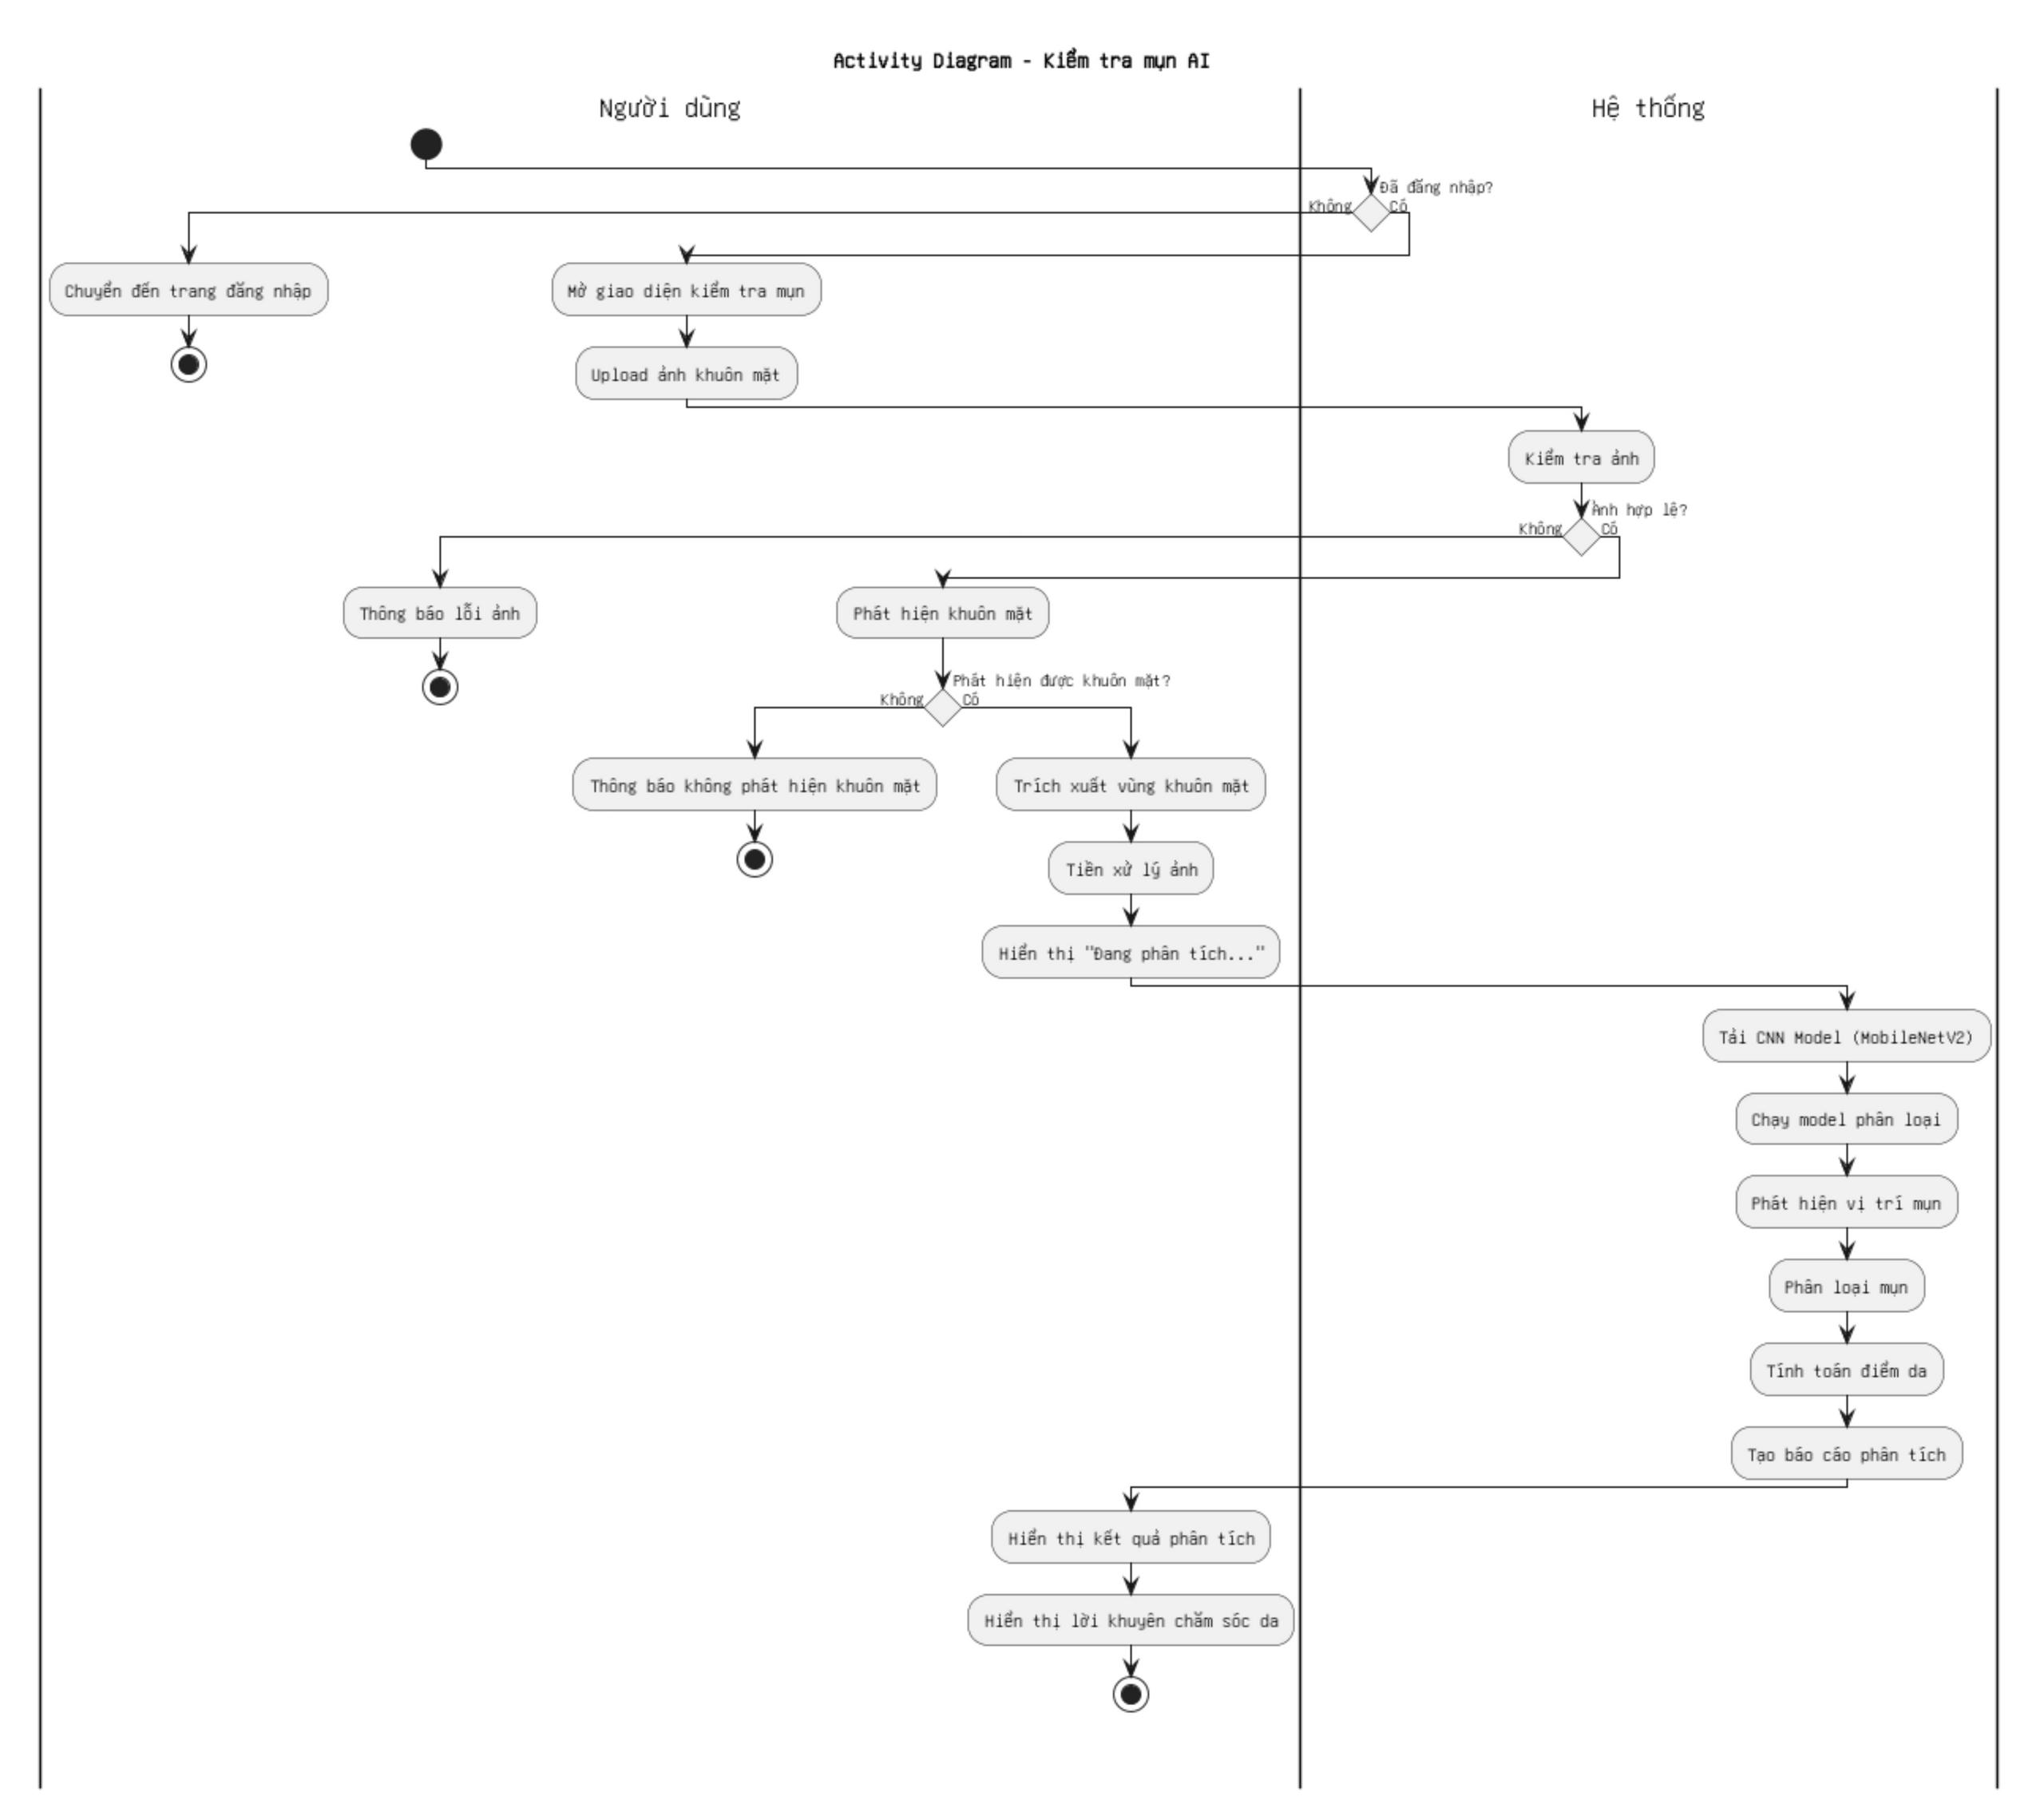
\includegraphics[width=0.8\textwidth]{figures/ac_mun.jpg}
    \caption{Activity Diagram xử lý AI kiểm tra da mặt}
    \label{fig:ac_mun}
\end{figure}


\textbf{Mục đích:} Cho phép người dùng sử dụng AI để phát hiện và phân tích tình trạng mụn trên khuôn mặt thông qua ảnh.

\textbf{Luồng hoạt động:}

\begin{itemize}
    \item Hệ thống kiểm tra đăng nhập:
    \begin{itemize}
        \item \textit{Nếu chưa đăng nhập:} Chuyển đến trang đăng nhập và kết thúc.
        \item \textit{Nếu đã đăng nhập:} Mở giao diện kiểm tra mụn.
    \end{itemize}
    \item Người dùng upload ảnh khuôn mặt.
    \item Hệ thống kiểm tra định dạng ảnh:
    \begin{itemize}
        \item \textit{Nếu không hợp lệ:} Thông báo lỗi ảnh và kết thúc.
        \item \textit{Nếu hợp lệ:} Phát hiện khuôn mặt.
    \end{itemize}
    \item Hệ thống phát hiện được khuôn mặt:
    \begin{itemize}
        \item \textit{Nếu không:} Thông báo không phát hiện khuôn mặt và kết thúc.
        \item \textit{Nếu có:} Trích xuất vùng khuôn mặt và tiền xử lý ảnh.
    \end{itemize}
    \item Hiển thị "Đang phân tích...".
    \item Hệ thống:
    \begin{itemize}
        \item Tải CNN Model (MobileNetV2)
        \item Chạy model phân loại
        \item Phát hiện vị trí mụn
        \item Phân loại mụn
        \item Tính toán điểm da
        \item Tạo báo cáo phân tích
    \end{itemize}
    \item Hiển thị kết quả phân tích.
    \item Hiển thị lời khuyên chăm sóc da.
    \item Kết thúc quy trình.
\end{itemize}

\subsection{Activity Diagram xử lý AI chatbot}
\begin{figure}[H]
    \centering
    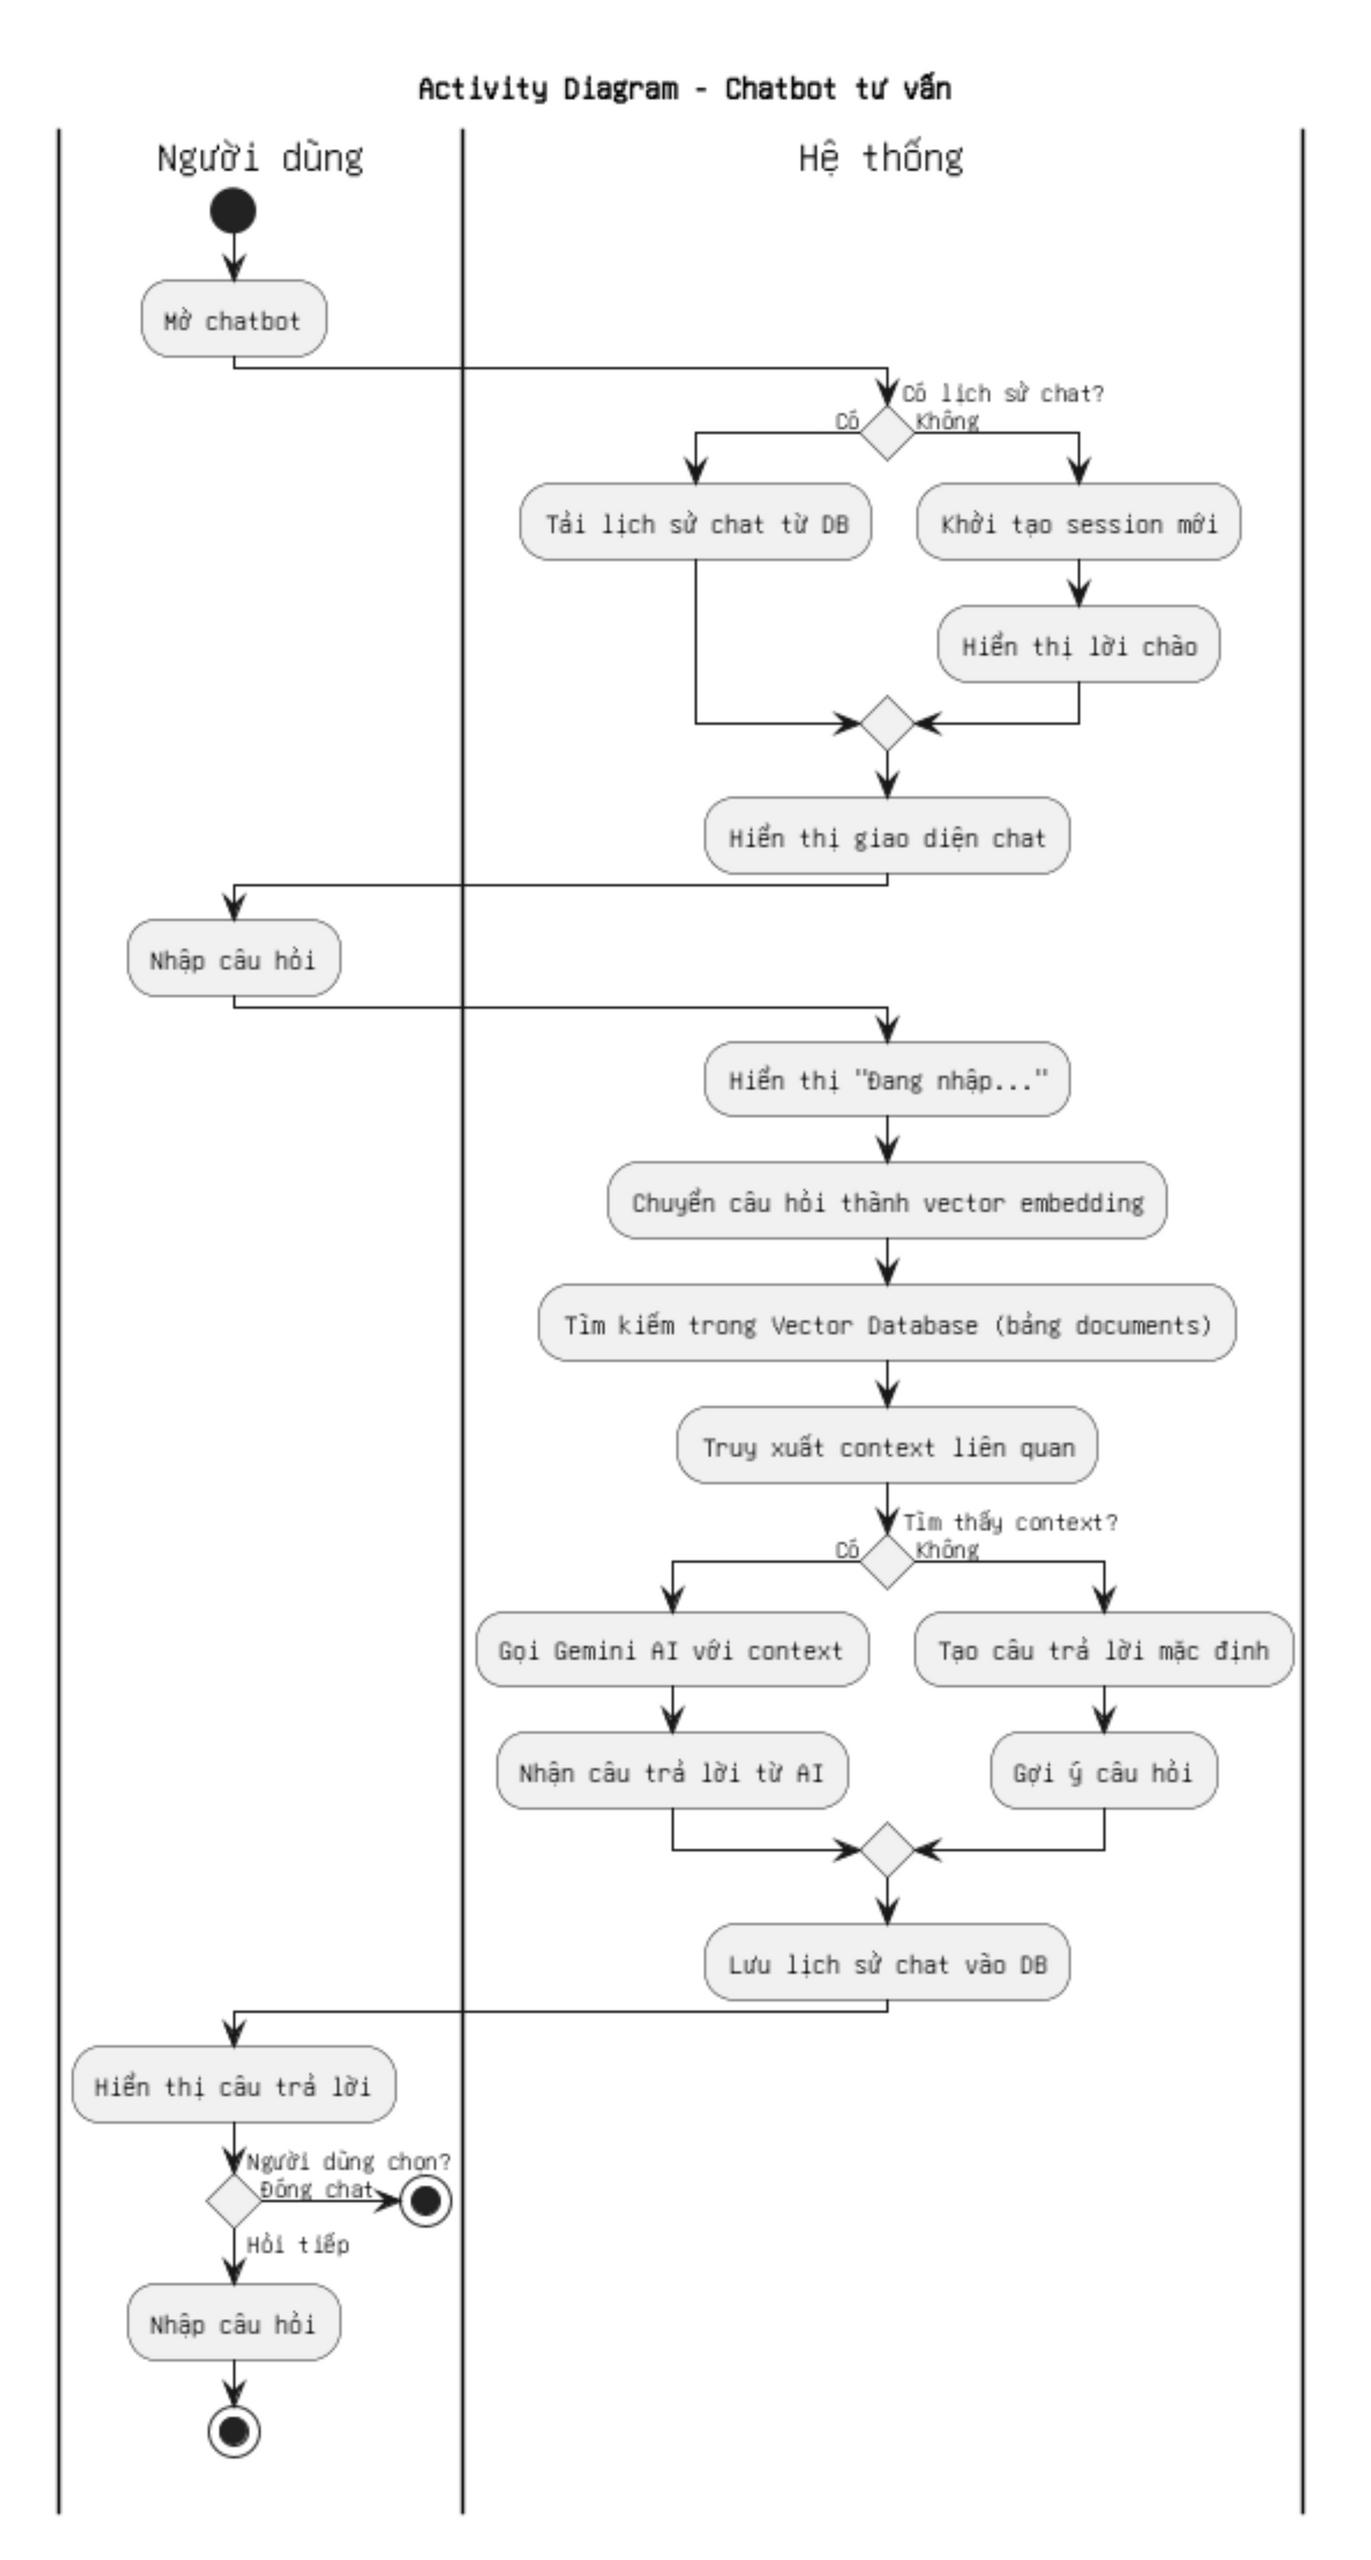
\includegraphics[width=0.5\textwidth]{figures/ac_tu_van.jpg}
    \caption{Activity Diagram xử lý AI chatbot}
    \label{fig:ac_chat}
\end{figure}

\textbf{Mục đích:} Cho phép người dùng tương tác với chatbot AI để được tư vấn về các dịch vụ cắt tóc, làm đẹp sử dụng công nghệ RAG (Retrieval-Augmented Generation).

\textbf{Luồng hoạt động:}

\begin{itemize}
    \item Người dùng mở chatbot.
    \item Hệ thống kiểm tra lịch sử chat:
    \begin{itemize}
        \item \textit{Nếu chưa có:} Tải lịch sử chat từ database.
        \item \textit{Nếu có:} Khởi tạo session mới và hiển thị lời chào.
    \end{itemize}
    \item Hiển thị giao diện chat.
    \item Người dùng nhập câu hỏi.
    \item Hệ thống hiển thị "Đang nhắp...".
    \item Chuyển câu hỏi thành vector embedding.
    \item Tìm kiếm trong Vector Database (bằng documents).
    \item Truy xuất context liên quan.
    \item Kiểm tra tìm thấy context:
    \begin{itemize}
        \item \textit{Nếu có:} Gọi Gemini AI với context.
        \item \textit{Nếu không:} Tạo câu trả lời mặc định.
    \end{itemize}
    \item Nhận câu trả lời từ AI và gửi ý câu hỏi.
    \item Lưu lịch sử chat vào database.
    \item Hiển thị câu trả lời.
    \item Kiểm tra người dùng chạy:
    \begin{itemize}
        \item \textit{Nếu chưa xong:} Quay lại bước nhập câu hỏi.
        \item \textit{Nếu xong:} Kết thúc quy trình.
    \end{itemize}
\end{itemize}



\subsection{Activity Diagram xử lý hợp tác}
\begin{figure}[H]
    \centering
    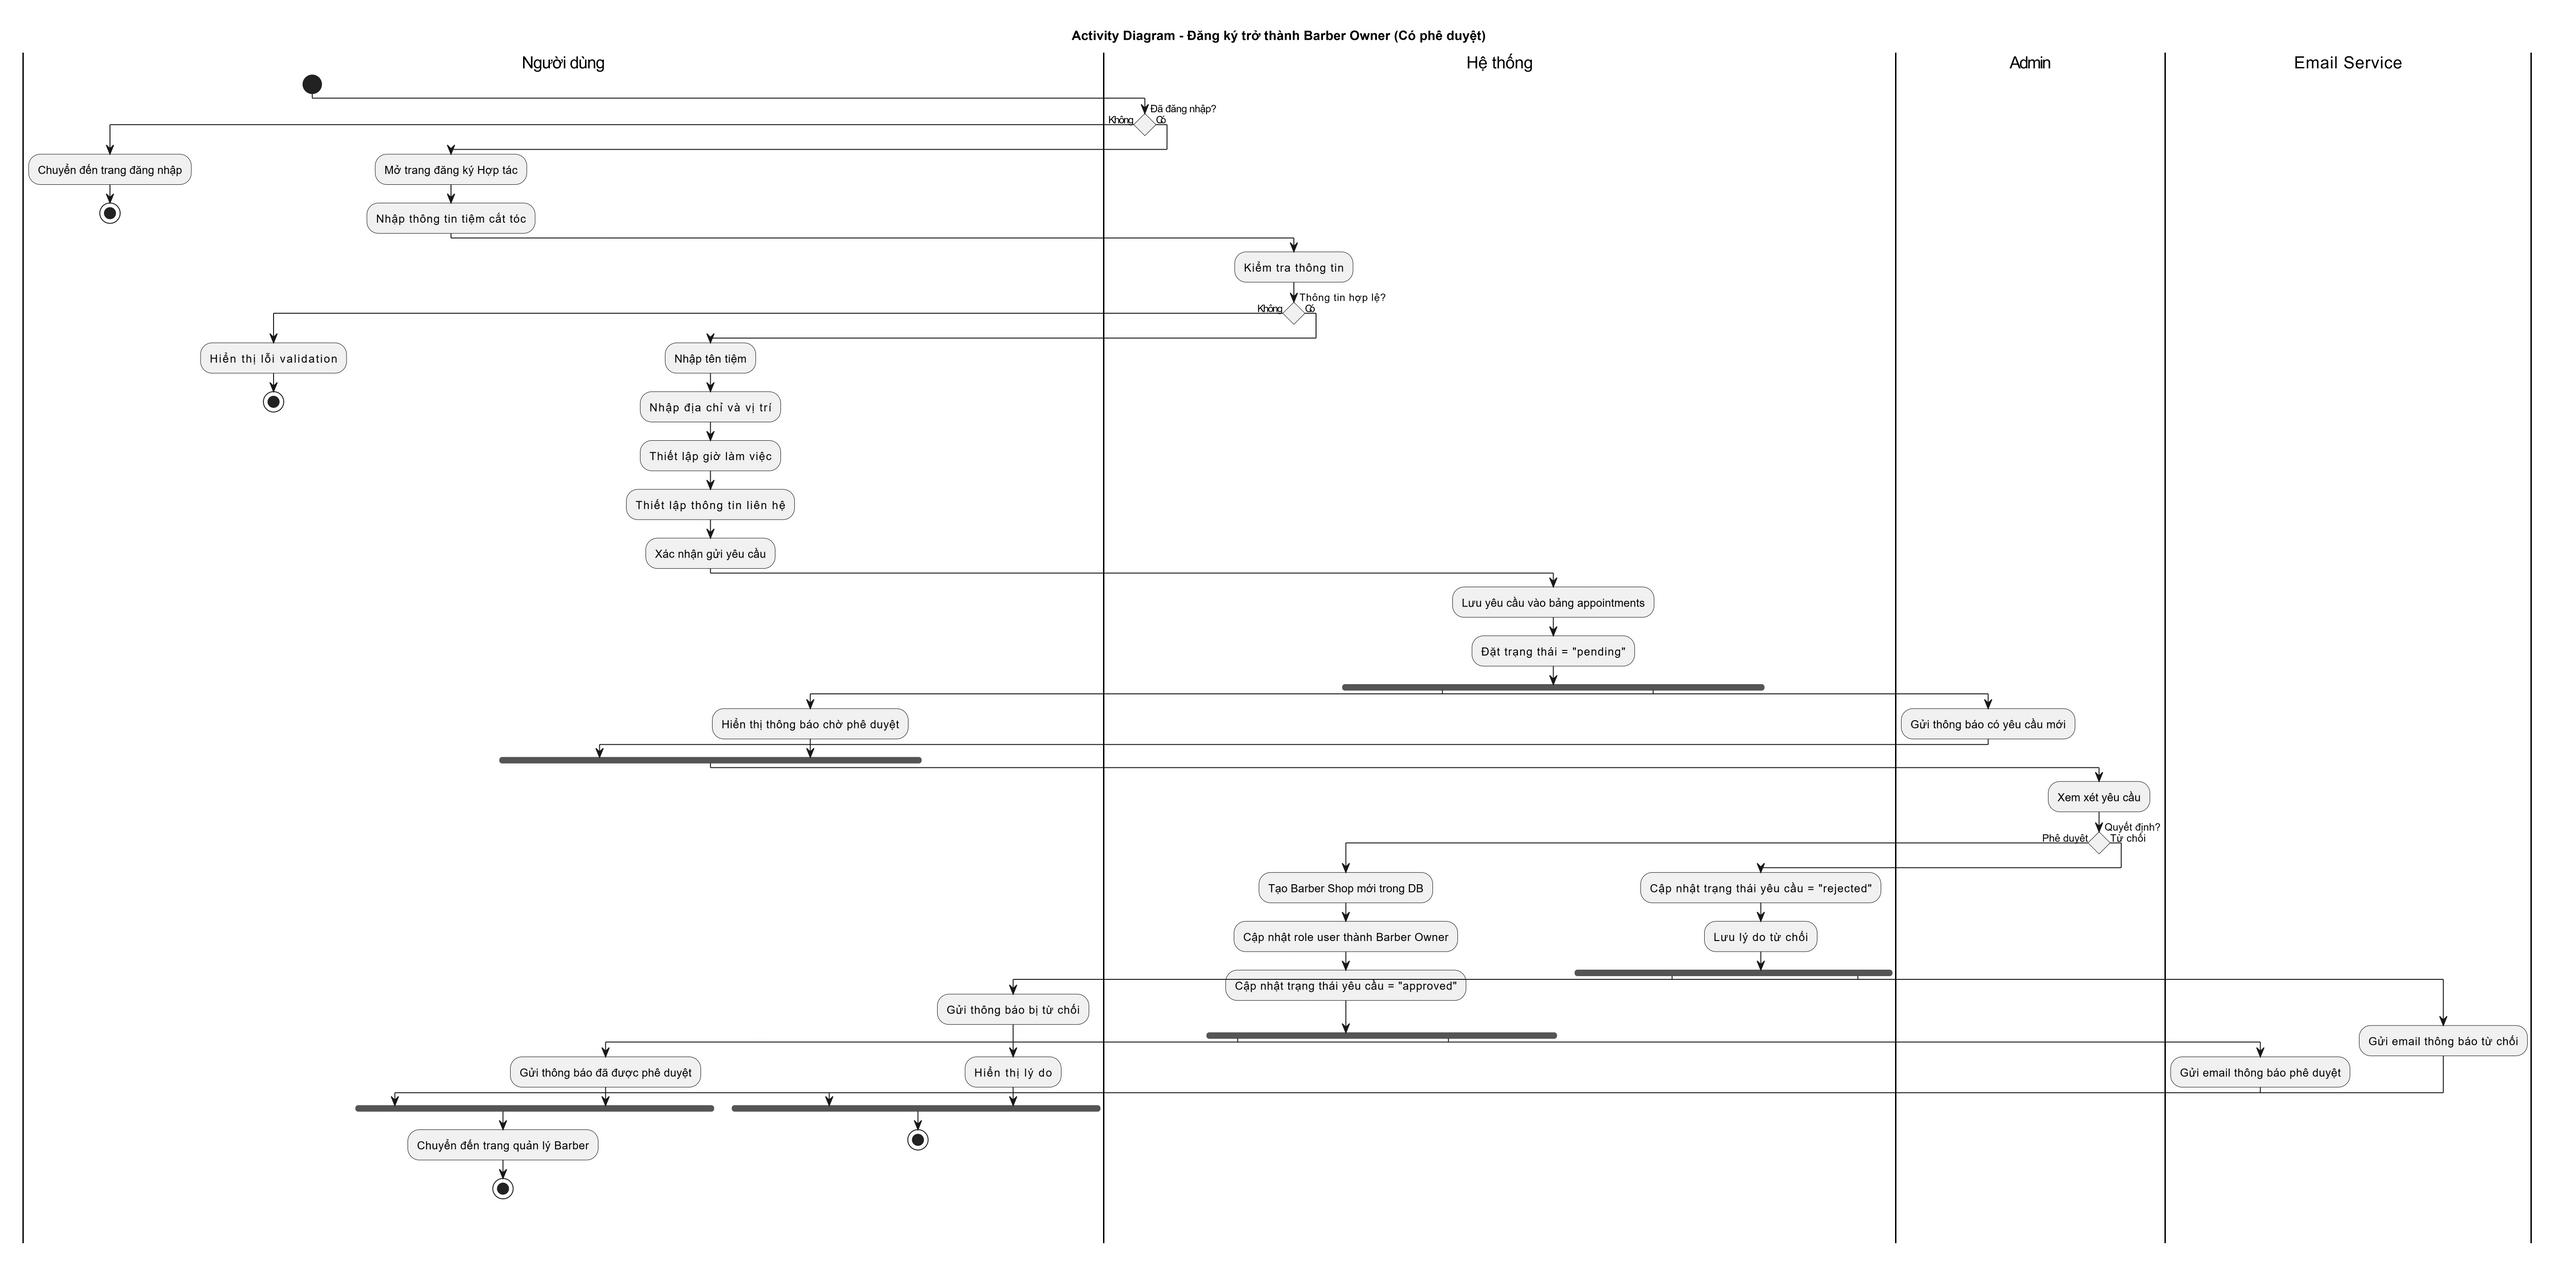
\includegraphics[width=0.8\textwidth]{figures/ac_hoptac_ok.jpg}
    \caption{Activity Diagram xử lý hợp tác}
    \label{fig:ac_hoptac}
\end{figure}


\textbf{Mục đích:} Cho phép người dùng đăng ký trở thành chủ tiệm cắt tóc thông qua quy trình xét duyệt từ Admin, bao gồm xác thực thông tin và phê duyệt hồ sơ.

\textbf{Luồng hoạt động:}

\begin{itemize}
    \item Hệ thống kiểm tra đăng nhập:
    \begin{itemize}
        \item \textit{Nếu chưa đăng nhập:} Chuyển đến trang đăng nhập và kết thúc.
        \item \textit{Nếu đã đăng nhập:} Mở trang đăng ký Hop tác.
    \end{itemize}
    \item Người dùng nhập thông tin hợp tác cắt tóc.
    \item Hệ thống kiểm tra thông tin đủ:
    \begin{itemize}
        \item \textit{Nếu không hợp đủ:} Hiển thị lỗi validation và kết thúc.
        \item \textit{Nếu đủ:} Nhập ảnh tiện.
    \end{itemize}
    \item Người dùng:
    \begin{itemize}
        \item Nhập ảnh chi vị trí
        \item Thiết lập giờ làm việc
        \item Thiết lập thông tin tiện hệ
        \item Xác nhận gửi yêu cầu
    \end{itemize}
    \item Hiển thị thông báo chờ phê duyệt.
    \item Admin:
    \begin{itemize}
        \item Lưu yêu cầu vào bảng appointments
        \item Đặt trạng thái = "pending"
    \end{itemize}
    \item Email Service gửi thông báo có yêu cầu mới.
    \item Admin xem sét yêu cầu và kiểm tra xét duyệt:
    \begin{itemize}
        \item \textit{Nếu từ chối:}
        \begin{itemize}
            \item Cập nhật trạng thái yêu cầu = "rejected"
            \item Lưu ý so từ chối
            \item Email Service gửi email thông báo từ chối
            \item Gửi email thông báo từ chối
            \item Gửi thông báo từ chối
            \item Hiển thị lý đủ
        \end{itemize}
        \item \textit{Nếu chấp nhận:}
        \begin{itemize}
            \item Tạo Barber Shop mới trong DB
            \item Cập nhật role user thành Barber Owner
            \item Cập nhật trạng thái yêu cầu = "approved"
            \item Gửi thông báo hô sở hợ phỉ duyệt
            \item Email Service gửi email thông báo phê duyệt
            \item Gửi email thông báo phê duyệt
        \end{itemize}
    \end{itemize}
    \item Gửi thông báo cho người phỉ duyệt.
    \item Chuyển đến trang quản lý Barber.
    \item Kết thúc quy trình.
\end{itemize}


\subsection{Activity Diagram cập nhật thông tin cá nhân người dùng}
\begin{figure}[H]
    \centering
    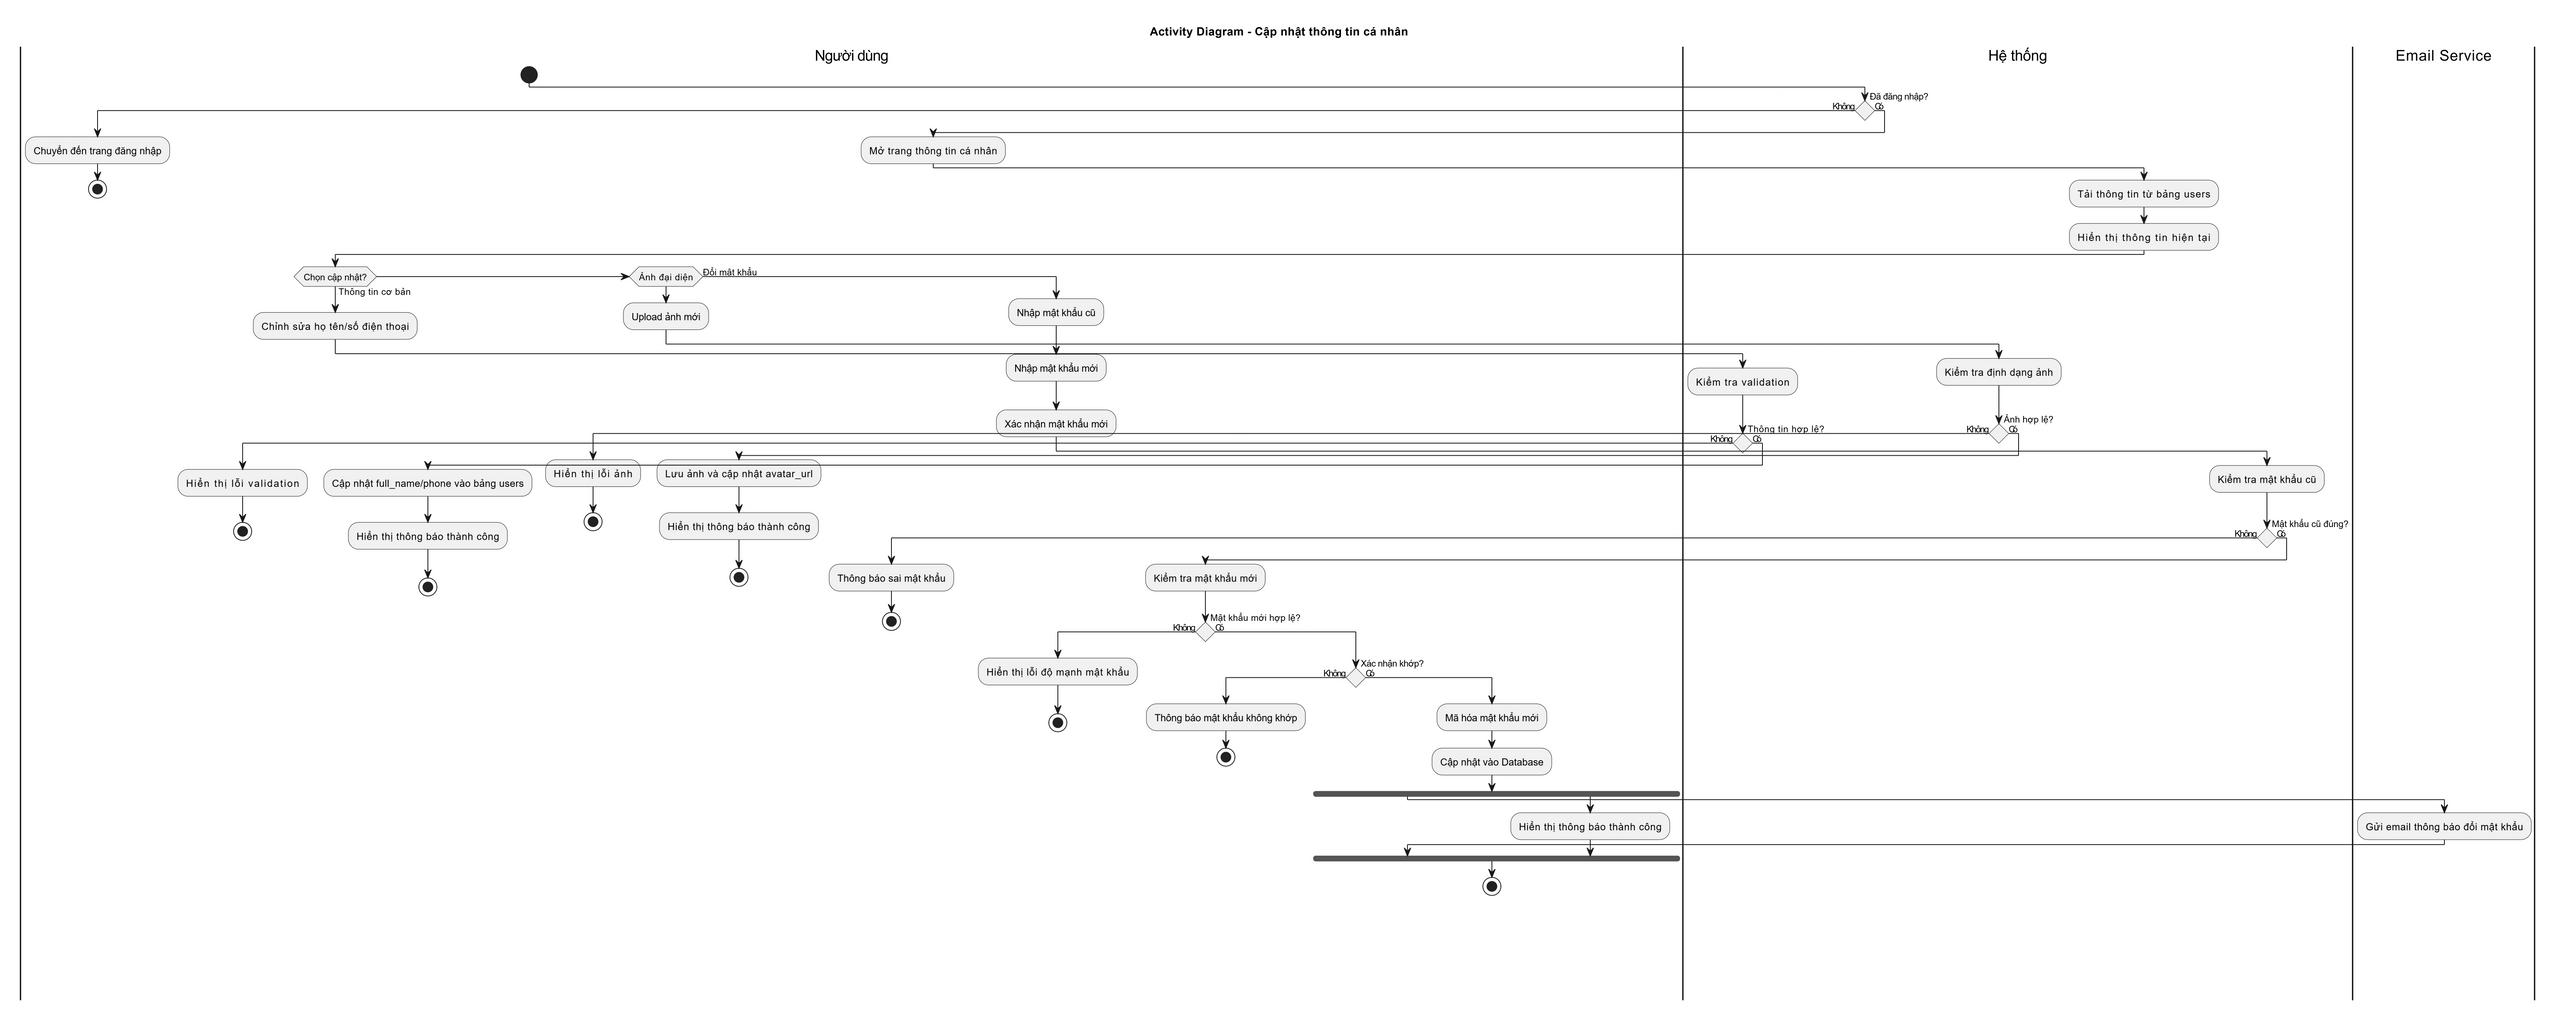
\includegraphics[width=0.8\textwidth]{figures/ac_update_profile.jpg}
    \caption{Activity Diagram cập nhật thông tin cá nhân}
    \label{fig:ac_update_profile}
\end{figure}


\textbf{Mục đích:} Cho phép người dùng cập nhật thông tin cá nhân bao gồm thông tin cơ bản, ảnh đại diện và đổi mật khẩu.

\textbf{Luồng hoạt động:}

\begin{itemize}
    \item Hệ thống kiểm tra đăng nhập:
    \begin{itemize}
        \item \textit{Nếu chưa đăng nhập:} Chuyển đến trang đăng nhập và kết thúc.
        \item \textit{Nếu đã đăng nhập:} Mở trang thông tin cá nhân.
    \end{itemize}
    \item Hệ thống tải thông tin từ bảng users và hiển thị thông tin hiện tại.
    \item Người dùng chọn loại cập nhật:
    
    \textbf{a) Thông tin cơ bản:}
    \begin{itemize}
        \item Chỉnh sửa họ tên/số điện thoại
        \item Hệ thống kiểm tra validation
        \item \textit{Nếu không hợp lệ:} Hiển thị lỗi validation và kết thúc
        \item \textit{Nếu hợp lệ:} Cập nhật full\_name/phone vào bảng users, hiển thị thông báo thành công
    \end{itemize}
    
    \textbf{b) Ảnh đại diện:}
    \begin{itemize}
        \item Upload ảnh mới
        \item Hệ thống kiểm tra định dạng ảnh
        \item \textit{Nếu không hợp lệ:} Hiển thị lỗi ảnh và kết thúc
        \item \textit{Nếu hợp lệ:} Lưu ảnh và cập nhật avatar\_url, hiển thị thông báo thành công
    \end{itemize}
    
    \textbf{c) Đổi mật khẩu:}
    \begin{itemize}
        \item Nhập mật khẩu cũ, mật khẩu mới và xác nhận mật khẩu mới
        \item Kiểm tra mật khẩu cũ đúng:
        \begin{itemize}
            \item \textit{Nếu sai:} Thông báo sai mật khẩu và kết thúc
            \item \textit{Nếu đúng:} Kiểm tra mật khẩu mới hợp lệ
        \end{itemize}
        \item Kiểm tra độ mạnh mật khẩu mới:
        \begin{itemize}
            \item \textit{Nếu không hợp lệ:} Hiển thị lỗi độ mạnh mật khẩu và kết thúc
            \item \textit{Nếu hợp lệ:} Kiểm tra xác nhận khớp
        \end{itemize}
        \item Kiểm tra xác nhận mật khẩu:
        \begin{itemize}
            \item \textit{Nếu không khớp:} Thông báo mật khẩu không khớp và kết thúc
            \item \textit{Nếu khớp:} Mã hóa mật khẩu mới, cập nhật vào database
        \end{itemize}
        \item Thực hiện song song:
        \begin{itemize}
            \item Email Service gửi email thông báo đổi mật khẩu
            \item Hiển thị thông báo thành công
        \end{itemize}
    \end{itemize}
\end{itemize}


\subsection{Activity Diagram tra cứu tiệm cắt tóc}
\begin{figure}[H]
    \centering
    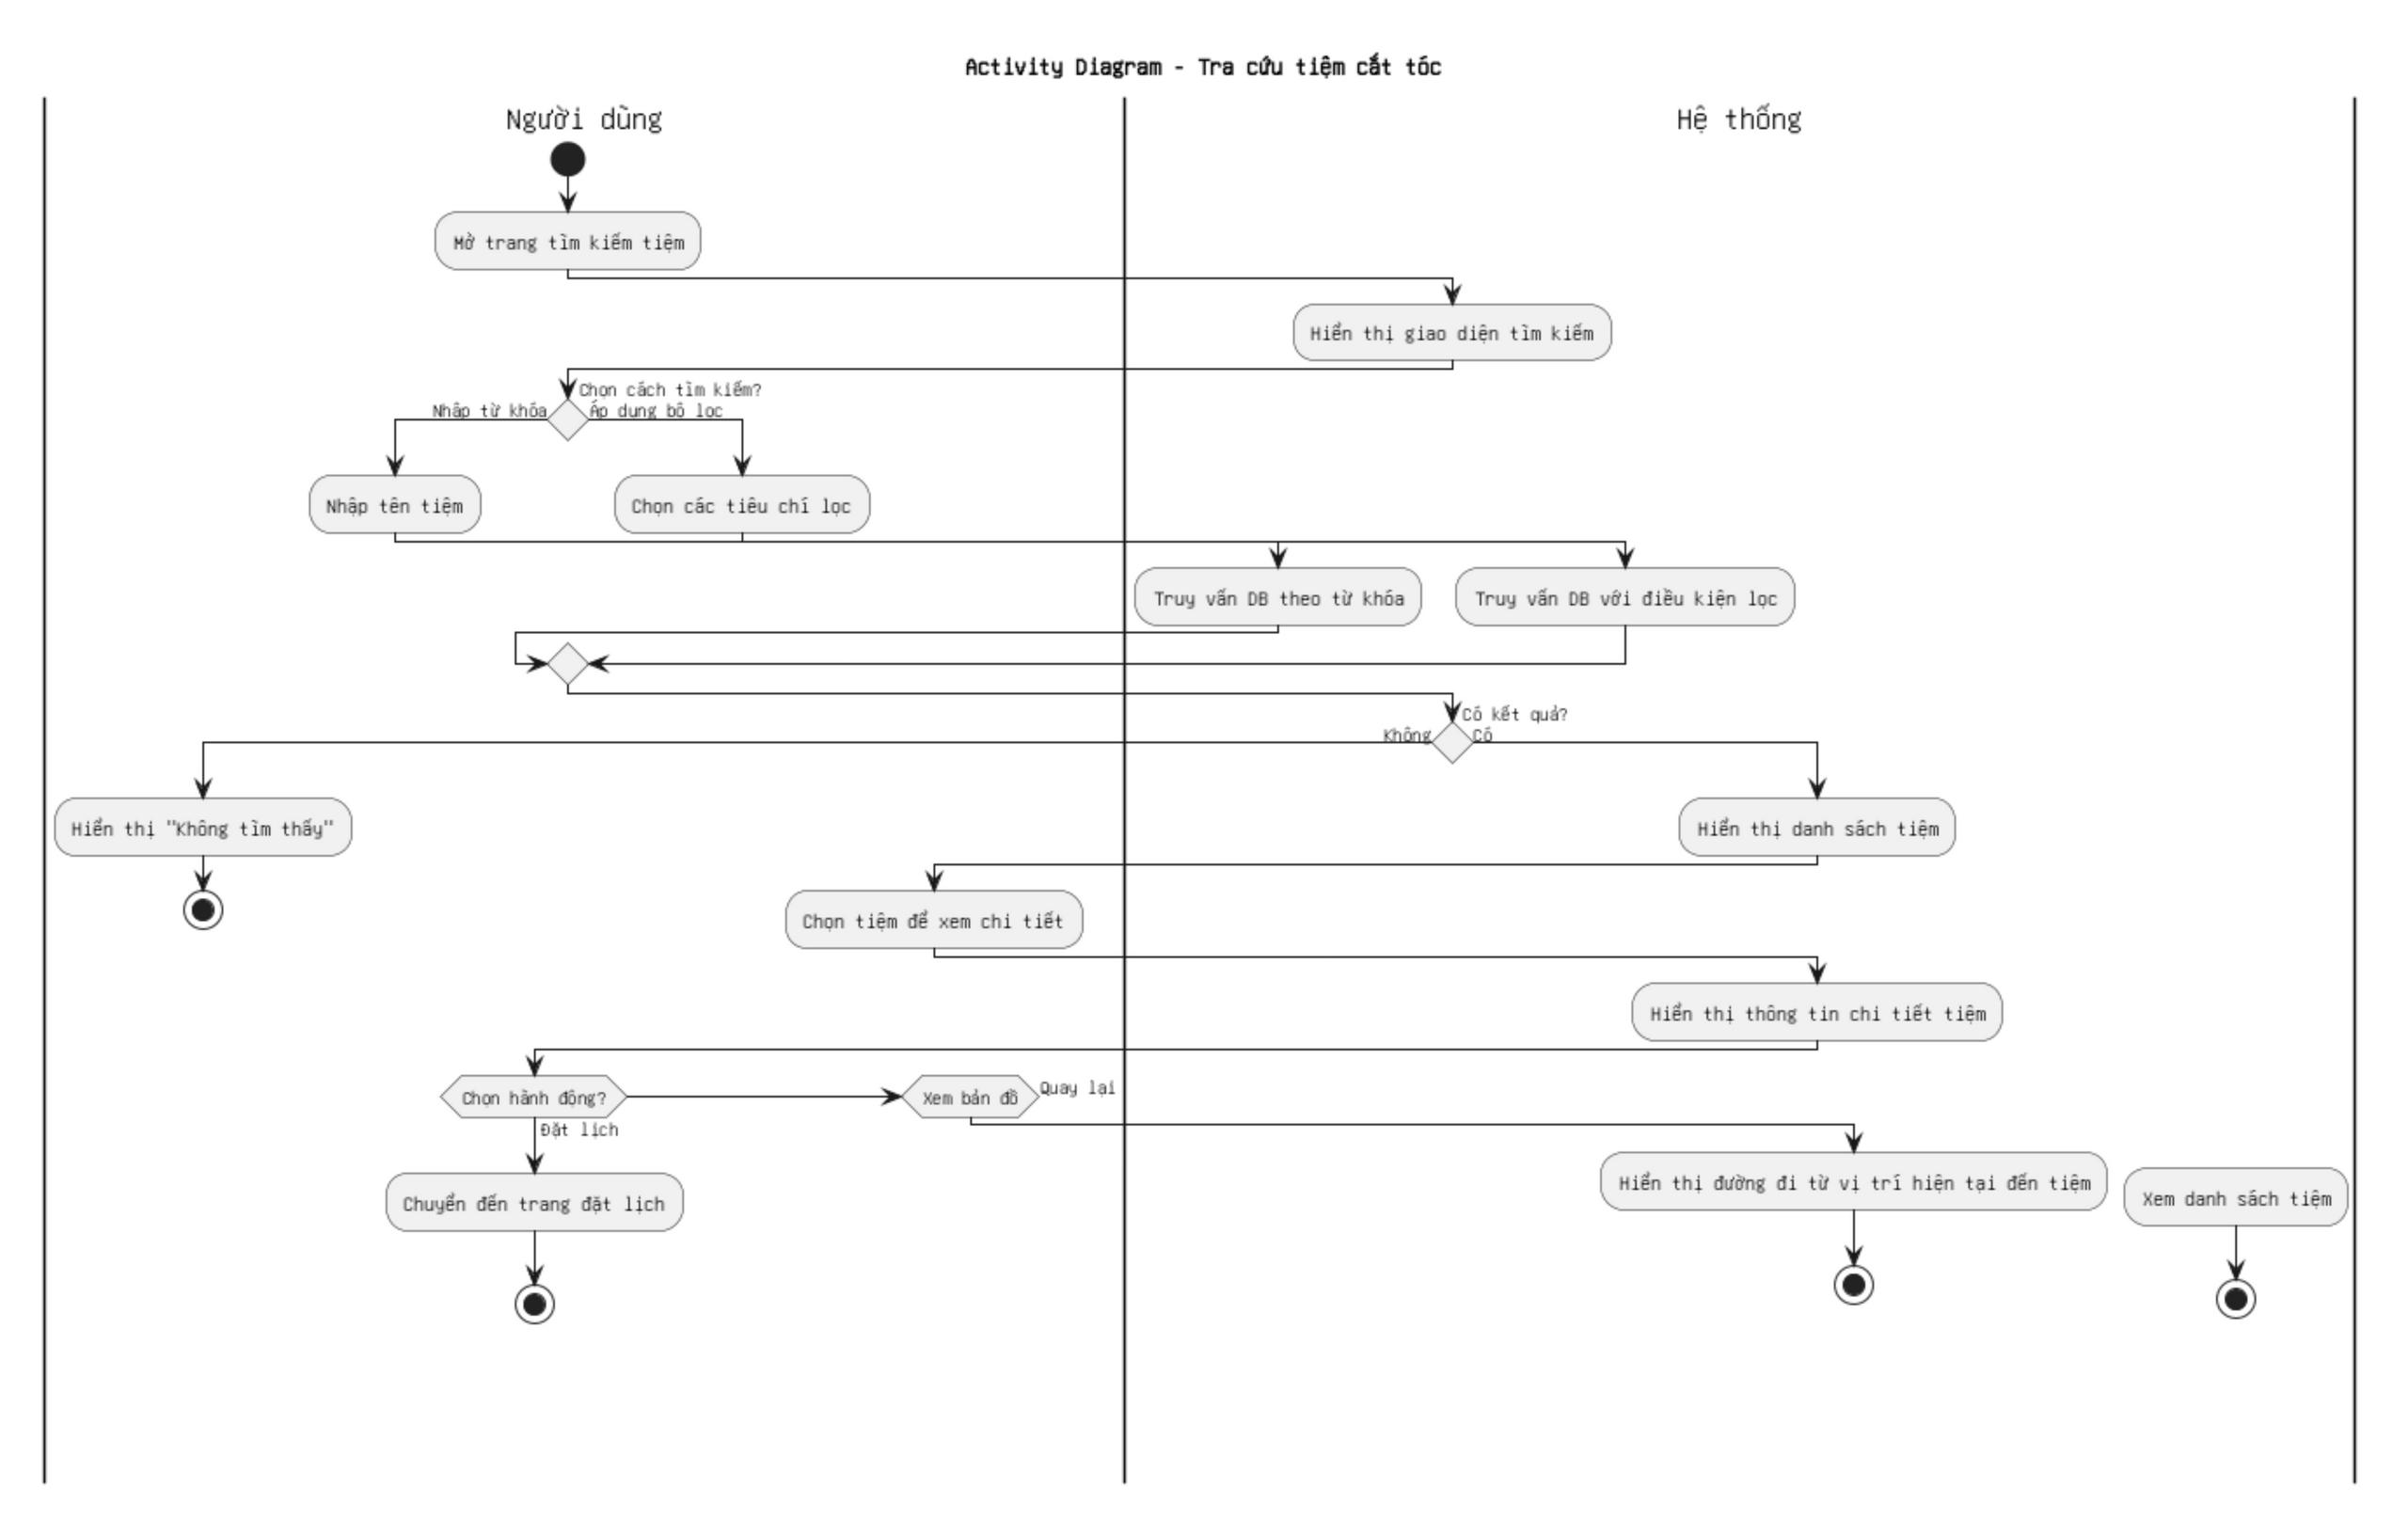
\includegraphics[width=1\textwidth]{figures/ac_tra_cuu.jpg}
    \caption{Activity Diagram tra cứu tiệm cắt tóc}
    \label{fig:ac_tra_cuu}
\end{figure}
\textbf{Mục đích:} Cho phép người dùng tìm kiếm và tra cứu thông tin các tiệm cắt tóc theo tên hoặc theo các tiêu chí lọc.

\textbf{Luồng hoạt động:}

\begin{itemize}
    \item Người dùng mở trang tìm kiếm tiệm.
    \item Hệ thống hiển thị giao diện tìm tiệm.
    \item Người dùng chọn cách tìm kiếm:
    
    \textbf{a) Nhập từ khóa:}
    \begin{itemize}
        \item Nhập tên tiệm
        \item Hệ thống truy vấn DB theo từ khóa
    \end{itemize}
    
    \textbf{b) Chọn các tiêu chí lọc:}
    \begin{itemize}
        \item Chọn các tiêu chí lọc
        \item Hệ thống truy vấn DB với điều kiện lọc
    \end{itemize}
    
    \item Hệ thống kiểm tra có kết quả:
    \begin{itemize}
        \item \textit{Nếu không:} Hiển thị "Không tìm thấy" và kết thúc.
        \item \textit{Nếu có:} Hiển thị danh sách tiệm.
    \end{itemize}
    
    \item Người dùng chọn tiệm để xem chi tiết.
    \item Hệ thống hiển thị thông tin chi tiết tiệm.
    \item Người dùng chọn hành động:
    \begin{itemize}
        \item \textit{Đặt lịch:} Chuyển đến trang đặt lịch và kết thúc.
        \item \textit{Quay lại:} Xem danh sách tiệm và kết thúc.
    \end{itemize}
    
    \item Hiển thị đường đi từ vị trí hiện tại đến tiệm và kết thúc.
\end{itemize}

\subsection{Activity Diagram cập nhật thông tin tiệm cắt tóc}
\begin{figure}[H]
    \centering
    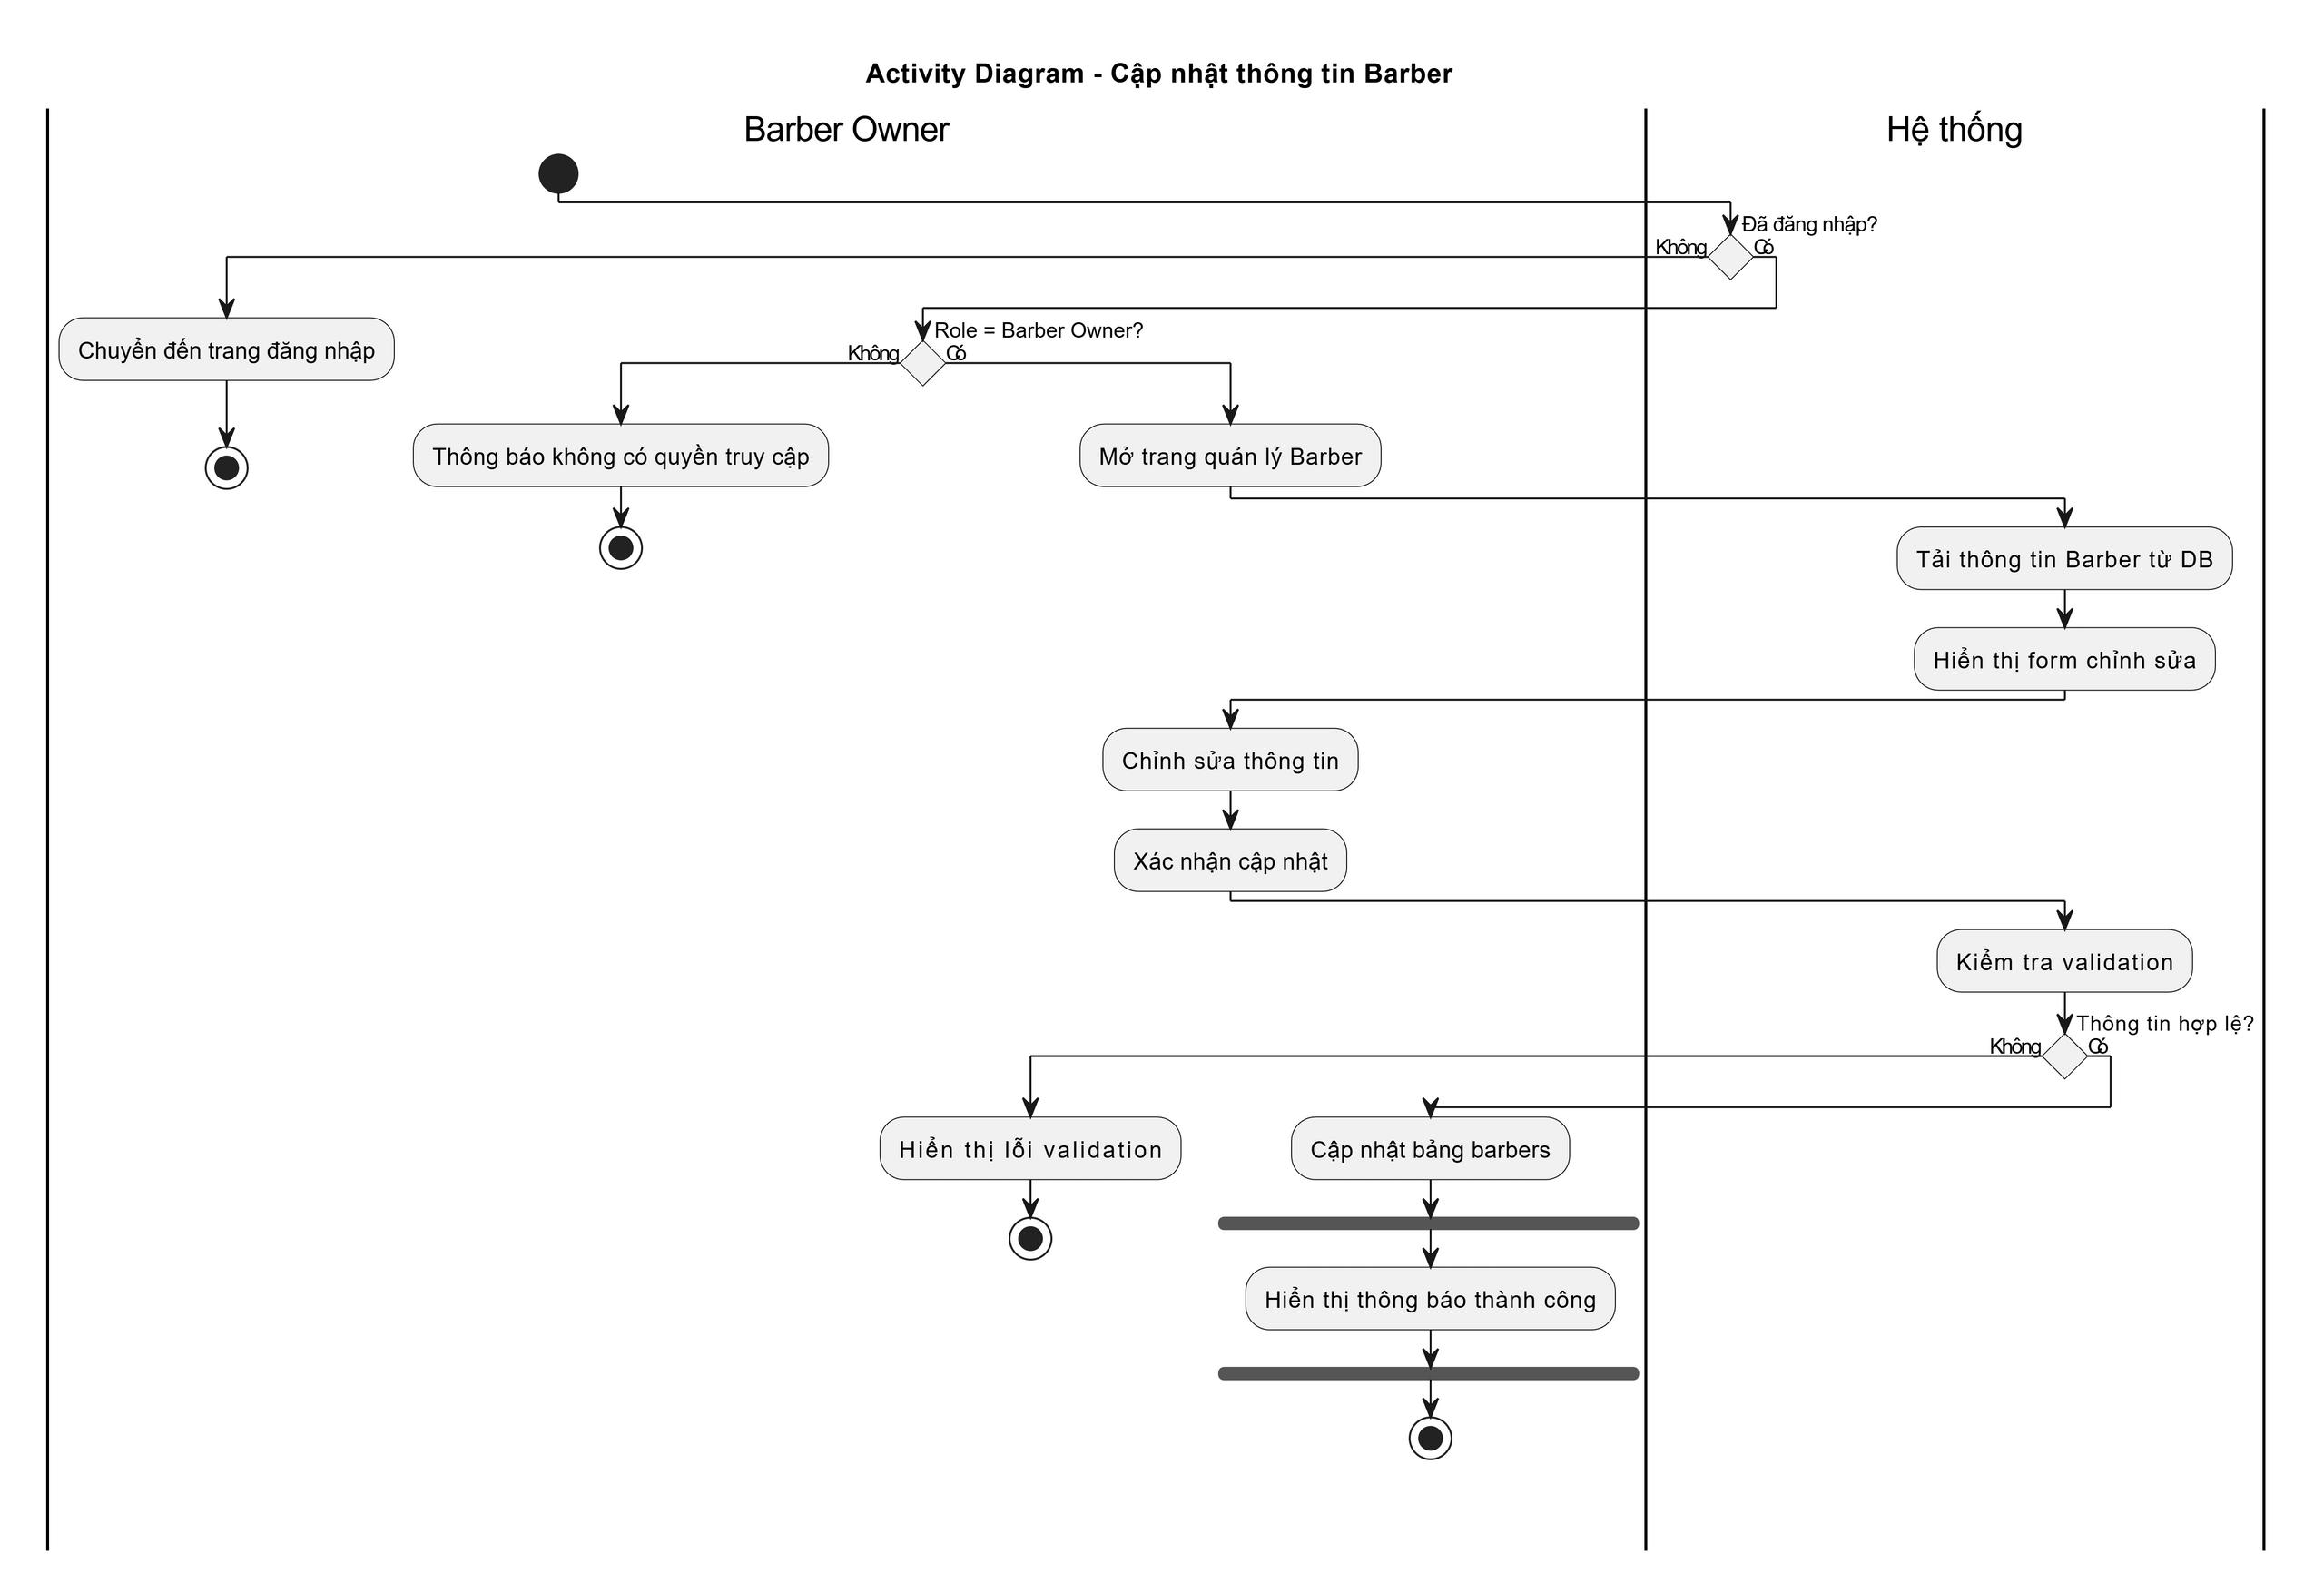
\includegraphics[width=1.2\textwidth]{figures/ac_update_ower.jpg}
    \caption{Activity Diagram cập nhật thông tin tiệm cắt tóc}
    \label{fig:ac_update_ower}
\end{figure}


\textbf{Mục đích:} Cho phép Barber Owner chỉnh sửa và cập nhật thông tin tiệm cắt tóc của mình trong hệ thống.

\textbf{Luồng hoạt động:}

\begin{itemize}
    \item Hệ thống kiểm tra đăng nhập:
    \begin{itemize}
        \item \textit{Nếu chưa đăng nhập:} Chuyển đến trang đăng nhập và kết thúc.
        \item \textit{Nếu đã đăng nhập:} Kiểm tra quyền truy cập.
    \end{itemize}
    
    \item Hệ thống kiểm tra Role = Barber Owner:
    \begin{itemize}
        \item \textit{Nếu không:} Thông báo không có quyền truy cập và kết thúc.
        \item \textit{Nếu có:} Mở trang quản lý Barber.
    \end{itemize}
    
    \item Hệ thống tải thông tin Barber từ DB và hiển thị form chỉnh sửa.
    
    \item Barber Owner chỉnh sửa thông tin.
    
    \item Barber Owner xác nhận cập nhật.
    
    \item Hệ thống kiểm tra validation:
    \begin{itemize}
        \item \textit{Nếu không hợp lệ:} Hiển thị lỗi validation và kết thúc.
        \item \textit{Nếu hợp lệ:} Cập nhật bảng barbers.
    \end{itemize}
    
    \item Hiển thị thông báo thành công.
    
    \item Kết thúc quy trình.
\end{itemize}

\subsection{Activity Diagram xem tài liệu RAG}
\begin{figure}[H]
    \centering
    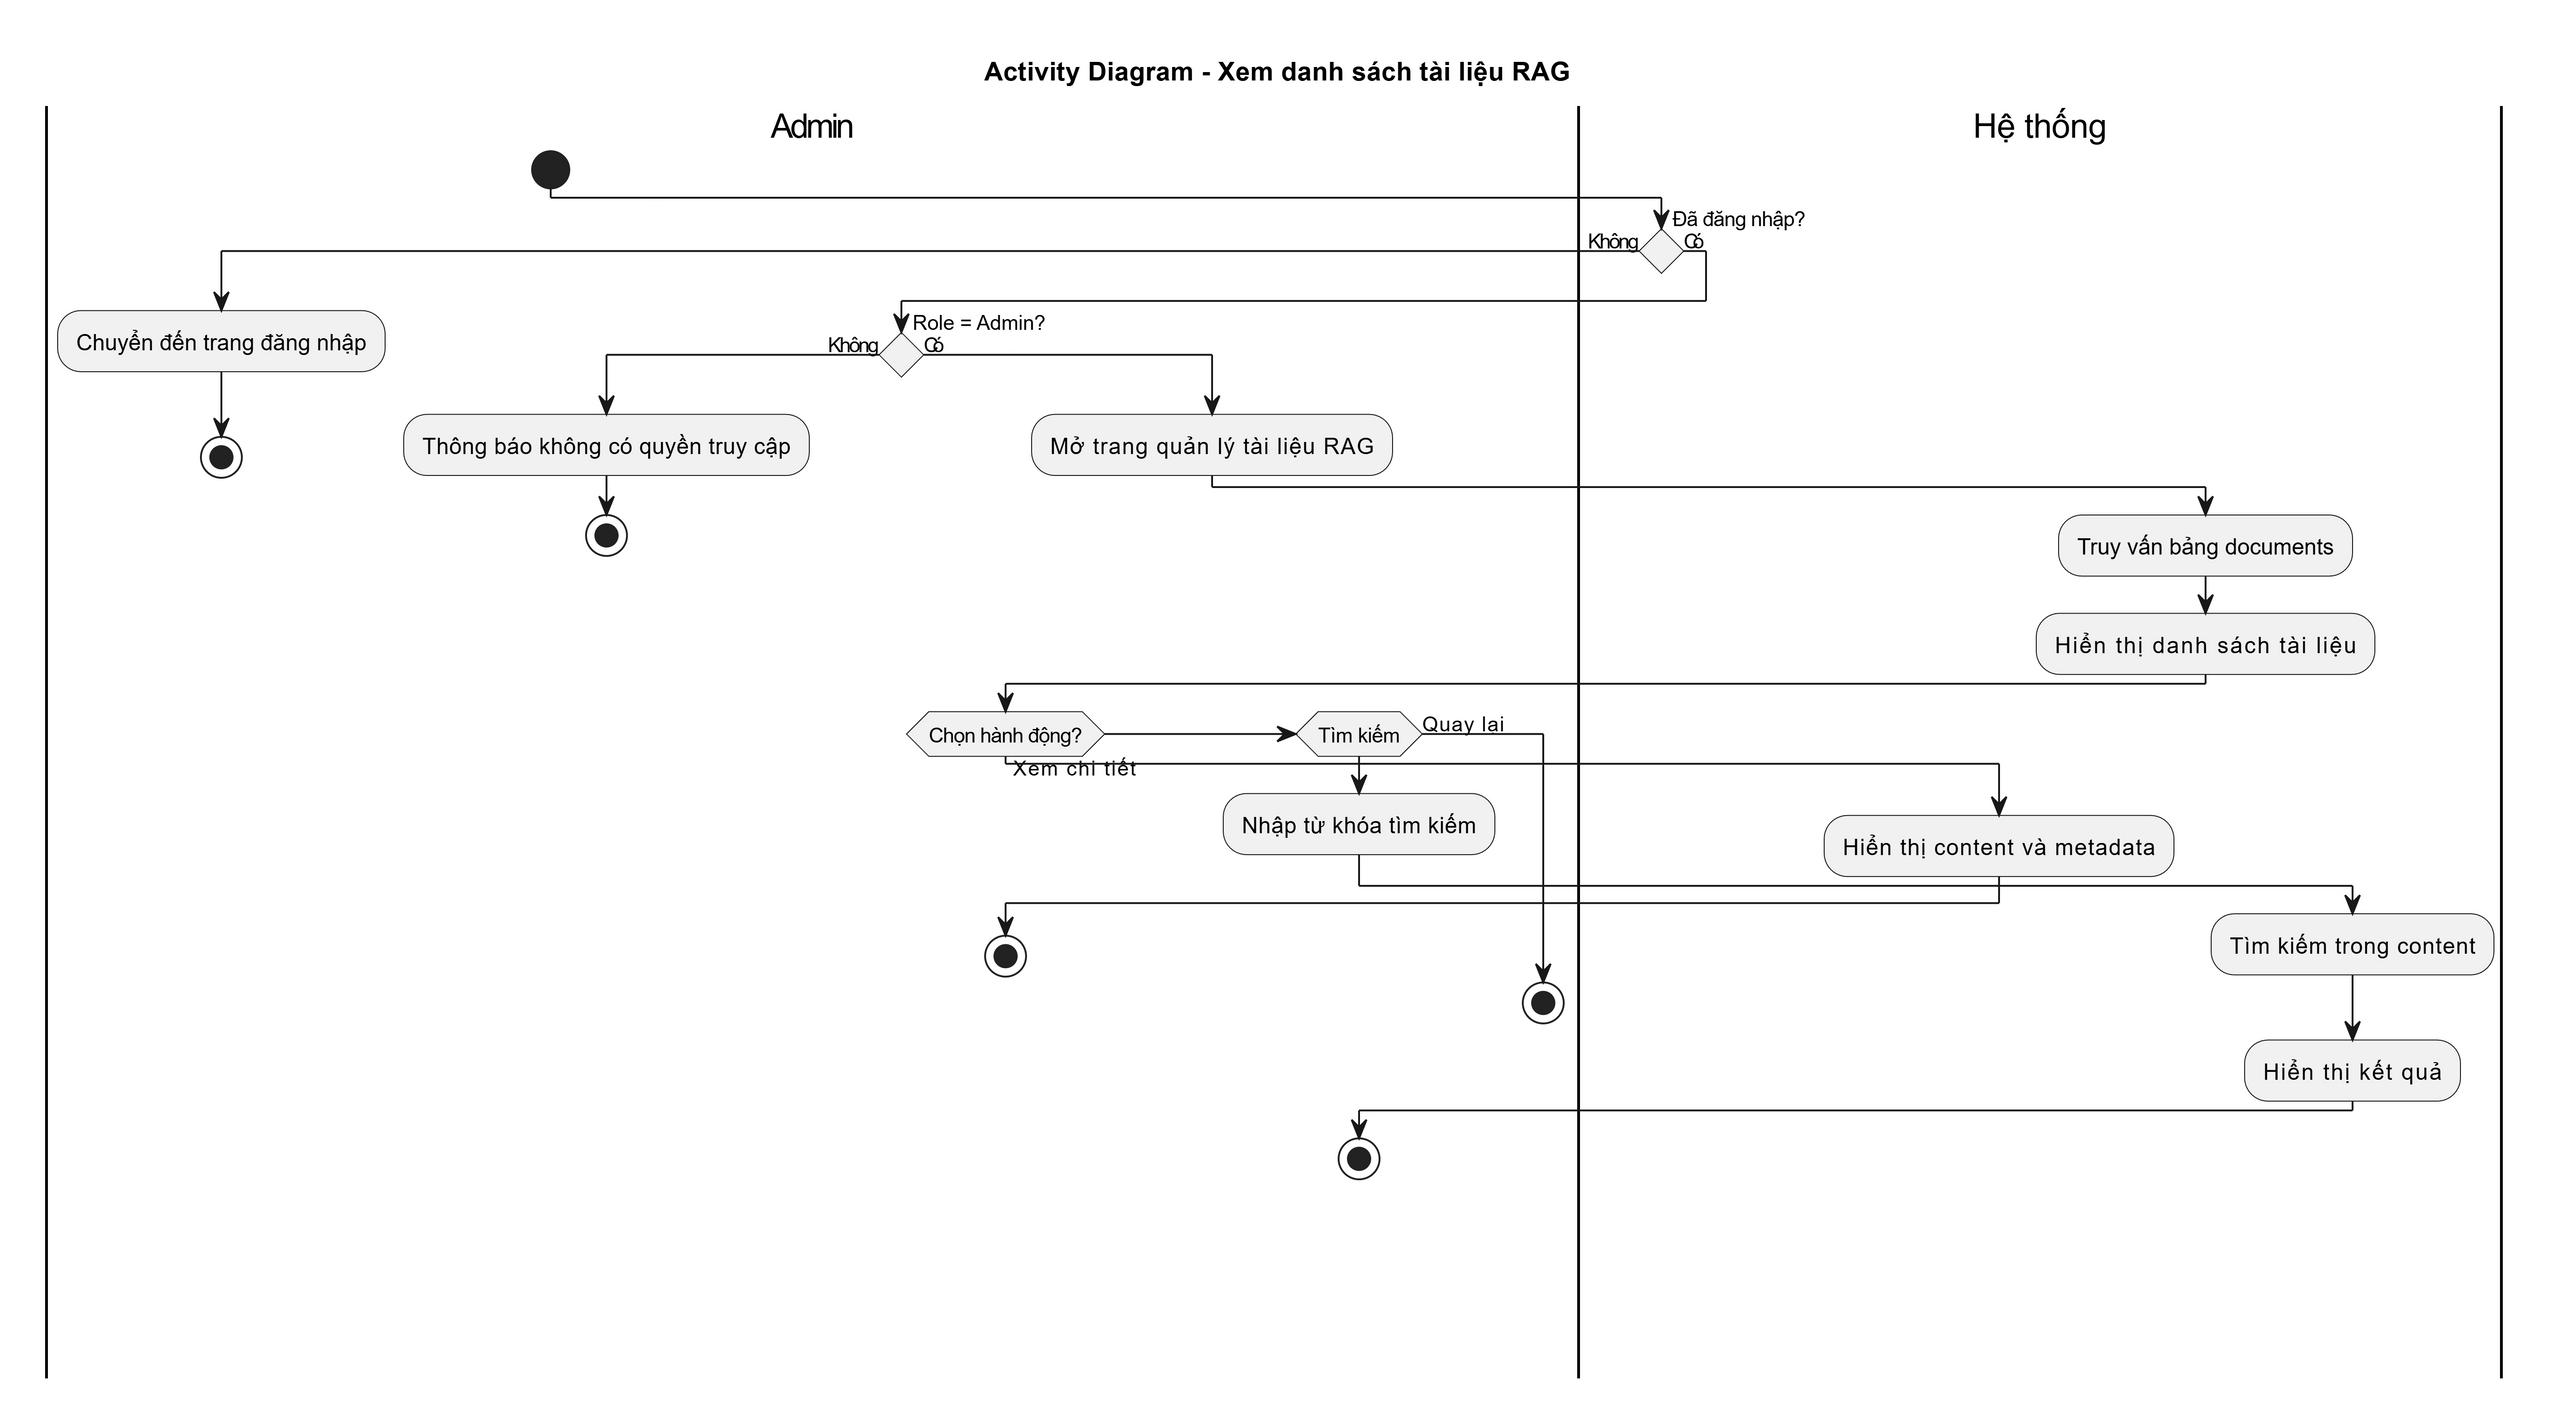
\includegraphics[width=0.8\textwidth]{figures/ac_rag.jpg}
    \caption{Activity Diagram xem tài liệu RAG}
    \label{fig:xem_rag}
\end{figure}

\textbf{Mục đích:} Cho phép Admin xem và quản lý danh sách tài liệu trong hệ thống RAG (Retrieval-Augmented Generation) để phục vụ chatbot tư vấn.

\textbf{Luồng hoạt động:}

\begin{itemize}
    \item Hệ thống kiểm tra đăng nhập:
    \begin{itemize}
        \item \textit{Nếu chưa đăng nhập:} Chuyển đến trang đăng nhập và kết thúc.
        \item \textit{Nếu đã đăng nhập:} Kiểm tra quyền truy cập.
    \end{itemize}
    
    \item Hệ thống kiểm tra Role = Admin:
    \begin{itemize}
        \item \textit{Nếu không:} Thông báo không có quyền truy cập và kết thúc.
        \item \textit{Nếu có:} Mở trang quản lý tài liệu RAG.
    \end{itemize}
    
    \item Hệ thống truy vấn bảng documents và hiển thị danh sách tài liệu.
    
    \item Admin chọn hành động:
    \begin{itemize}
        \item \textit{Xem chi tiết:}
        \begin{itemize}
            \item Hiển thị content và metadata
            \item Tìm kiếm trong content
            \item Hiển thị kết quả
            \item Kết thúc
        \end{itemize}
        \item \textit{Tìm kiếm:}
        \begin{itemize}
            \item Nhập từ khóa tìm kiếm
            \item Kết thúc
        \end{itemize}
        \item \textit{Quay lại:} Kết thúc
    \end{itemize}
\end{itemize}

\subsection{Activity Diagram tạo vector database}
\begin{figure}[H]
    \centering
    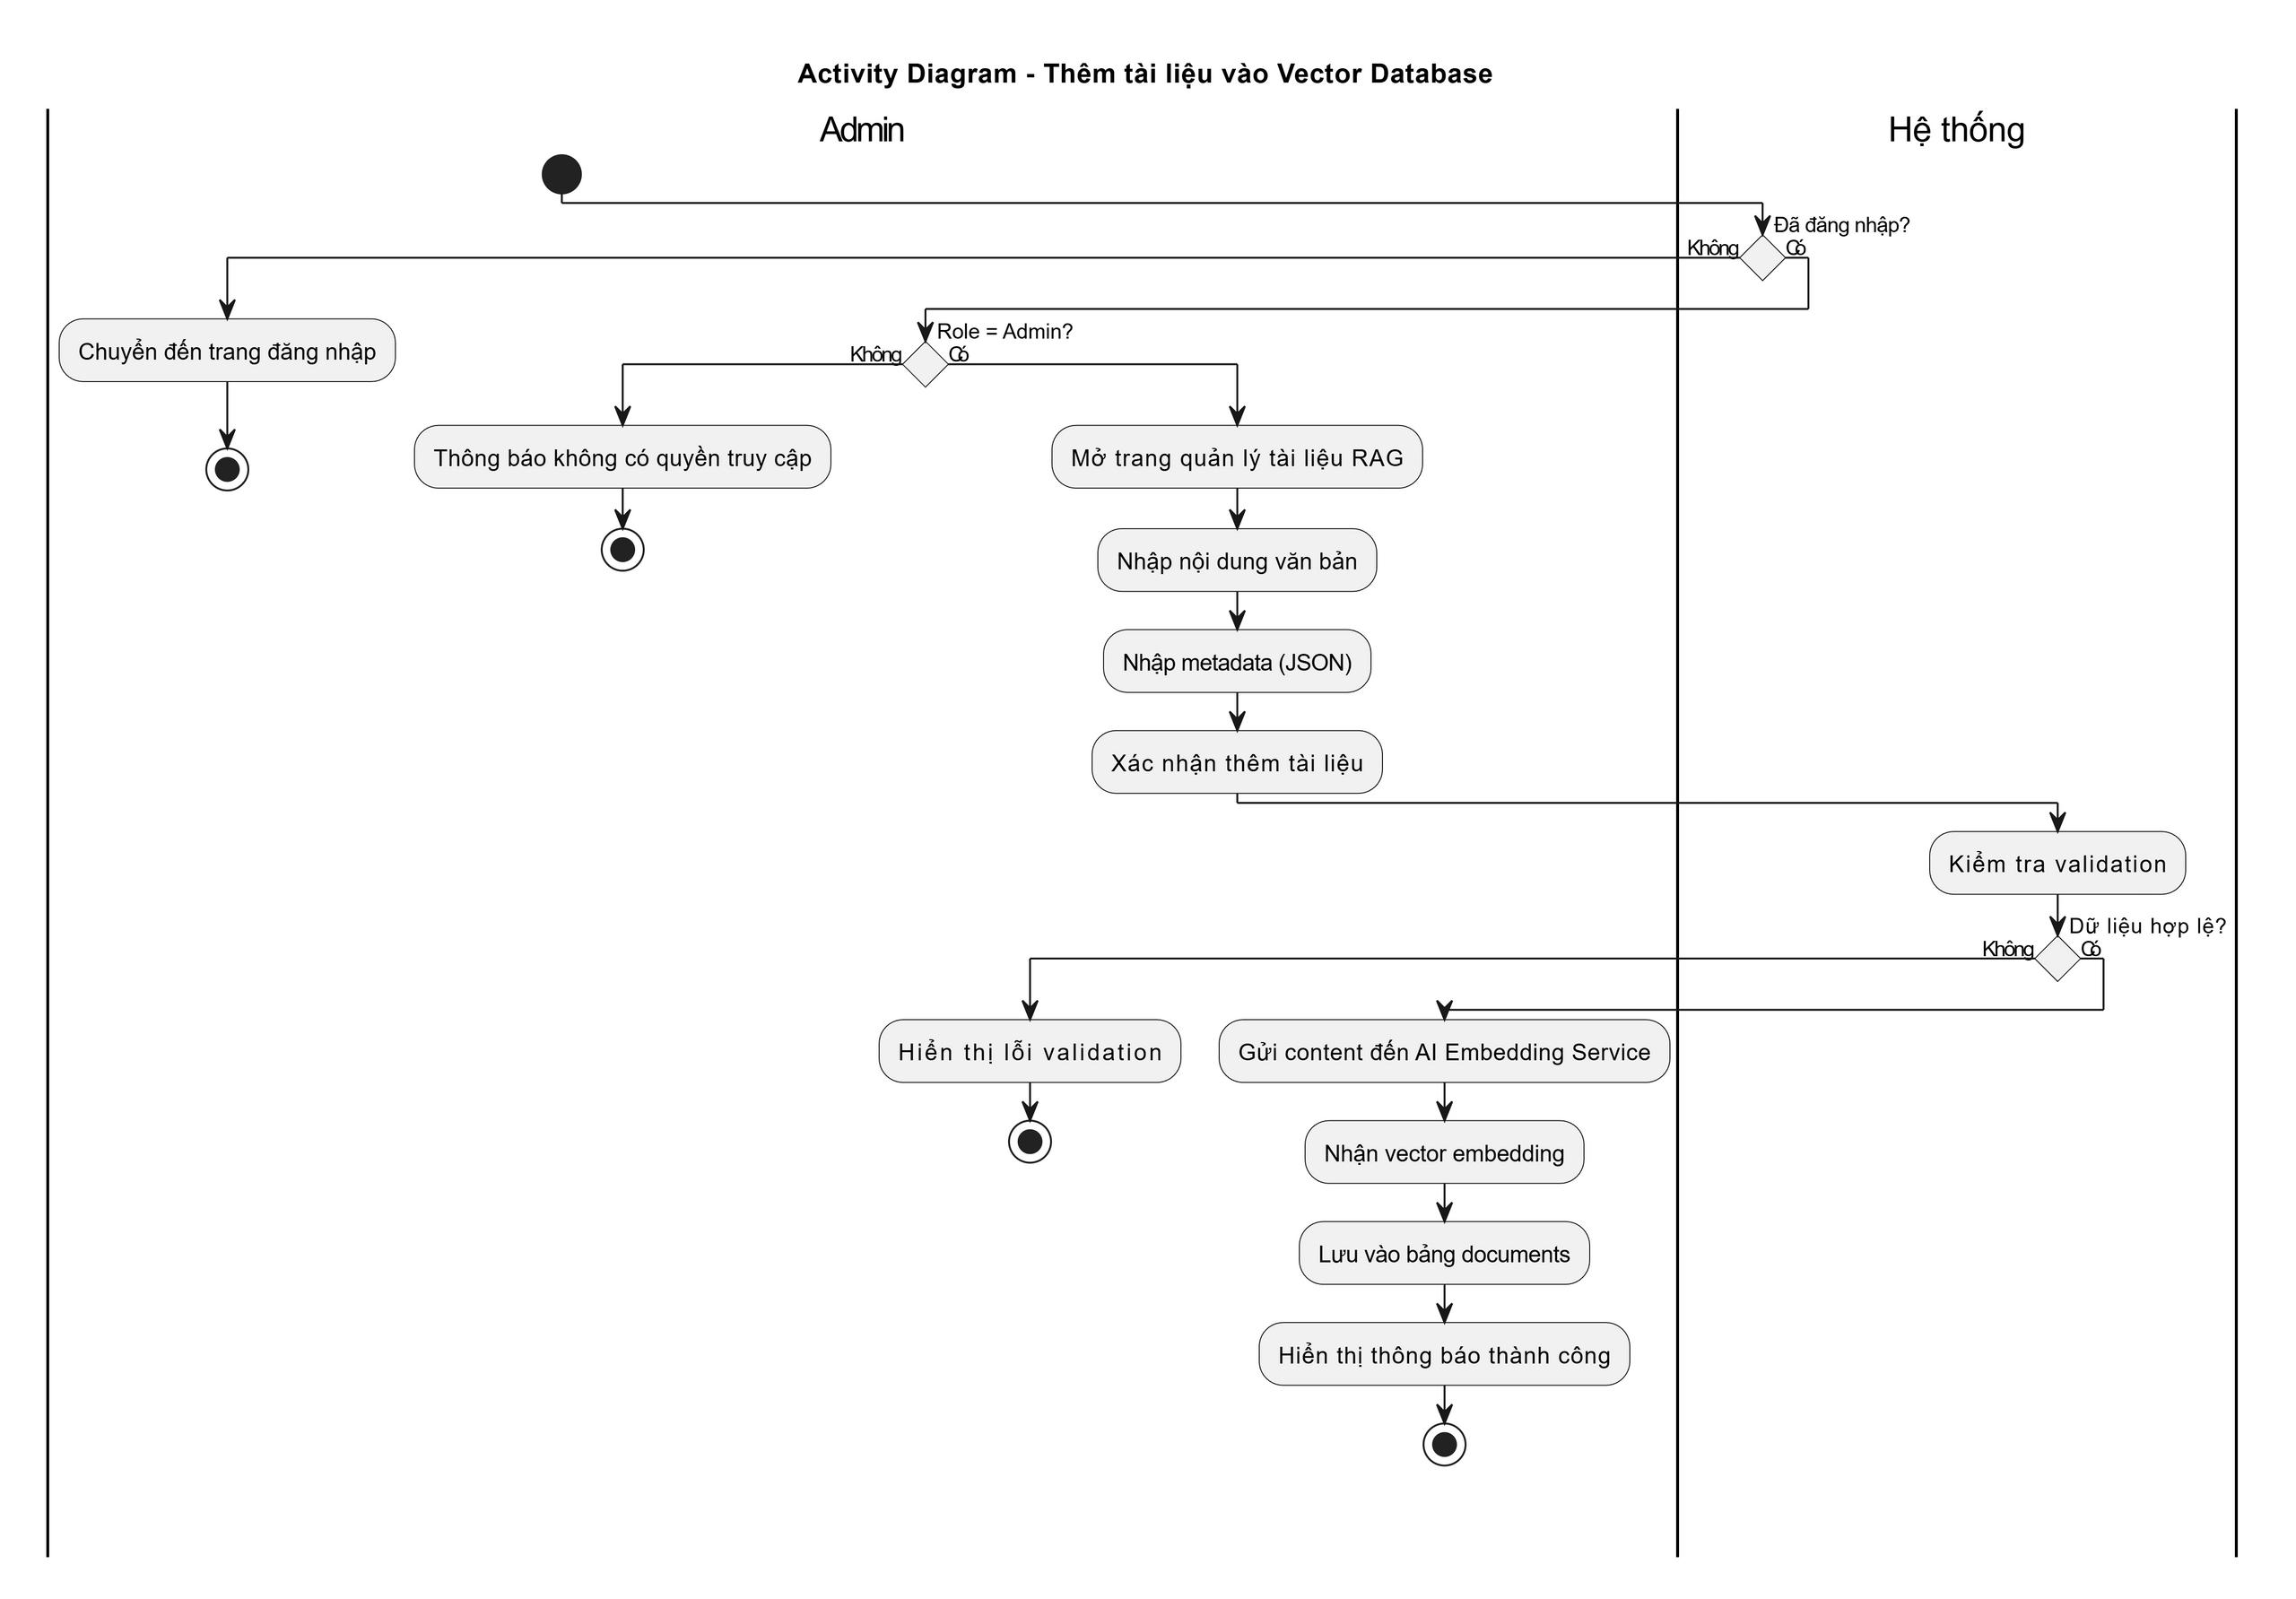
\includegraphics[width=0.8\textwidth]{figures/ac_vecto_database.jpg}
    \caption{Activity Diagram tạo vector database}
    \label{fig:ac_vector_db}
\end{figure}

\textbf{Mục đích:} Cho phép Admin thêm tài liệu mới vào Vector Database để tăng cường khả năng tư vấn của chatbot RAG.

\textbf{Luồng hoạt động:}

\begin{itemize}
    \item Hệ thống kiểm tra đăng nhập:
    \begin{itemize}
        \item \textit{Nếu chưa đăng nhập:} Chuyển đến trang đăng nhập và kết thúc.
        \item \textit{Nếu đã đăng nhập:} Kiểm tra quyền truy cập.
    \end{itemize}
    
    \item Hệ thống kiểm tra Role = Admin:
    \begin{itemize}
        \item \textit{Nếu không:} Thông báo không có quyền truy cập và kết thúc.
        \item \textit{Nếu có:} Mở trang quản lý tài liệu RAG.
    \end{itemize}
    
    \item Admin nhập nội dung văn bản.
    
    \item Admin nhập metadata (JSON).
    
    \item Admin xác nhận thêm tài liệu.
    
    \item Hệ thống kiểm tra validation:
    \begin{itemize}
        \item \textit{Nếu không hợp lệ:} Hiển thị lỗi validation và kết thúc.
        \item \textit{Nếu hợp lệ:} Gửi content đến AI Embedding Service.
    \end{itemize}
    
    \item Nhận vector embedding từ AI service.
    
    \item Lưu vào bảng documents.
    
    \item Hiển thị thông báo thành công.
    
    \item Kết thúc quy trình.
\end{itemize}

\subsection{Activity Diagram cập nhật tài liệu RAG}
\begin{figure}[H]
    \centering
    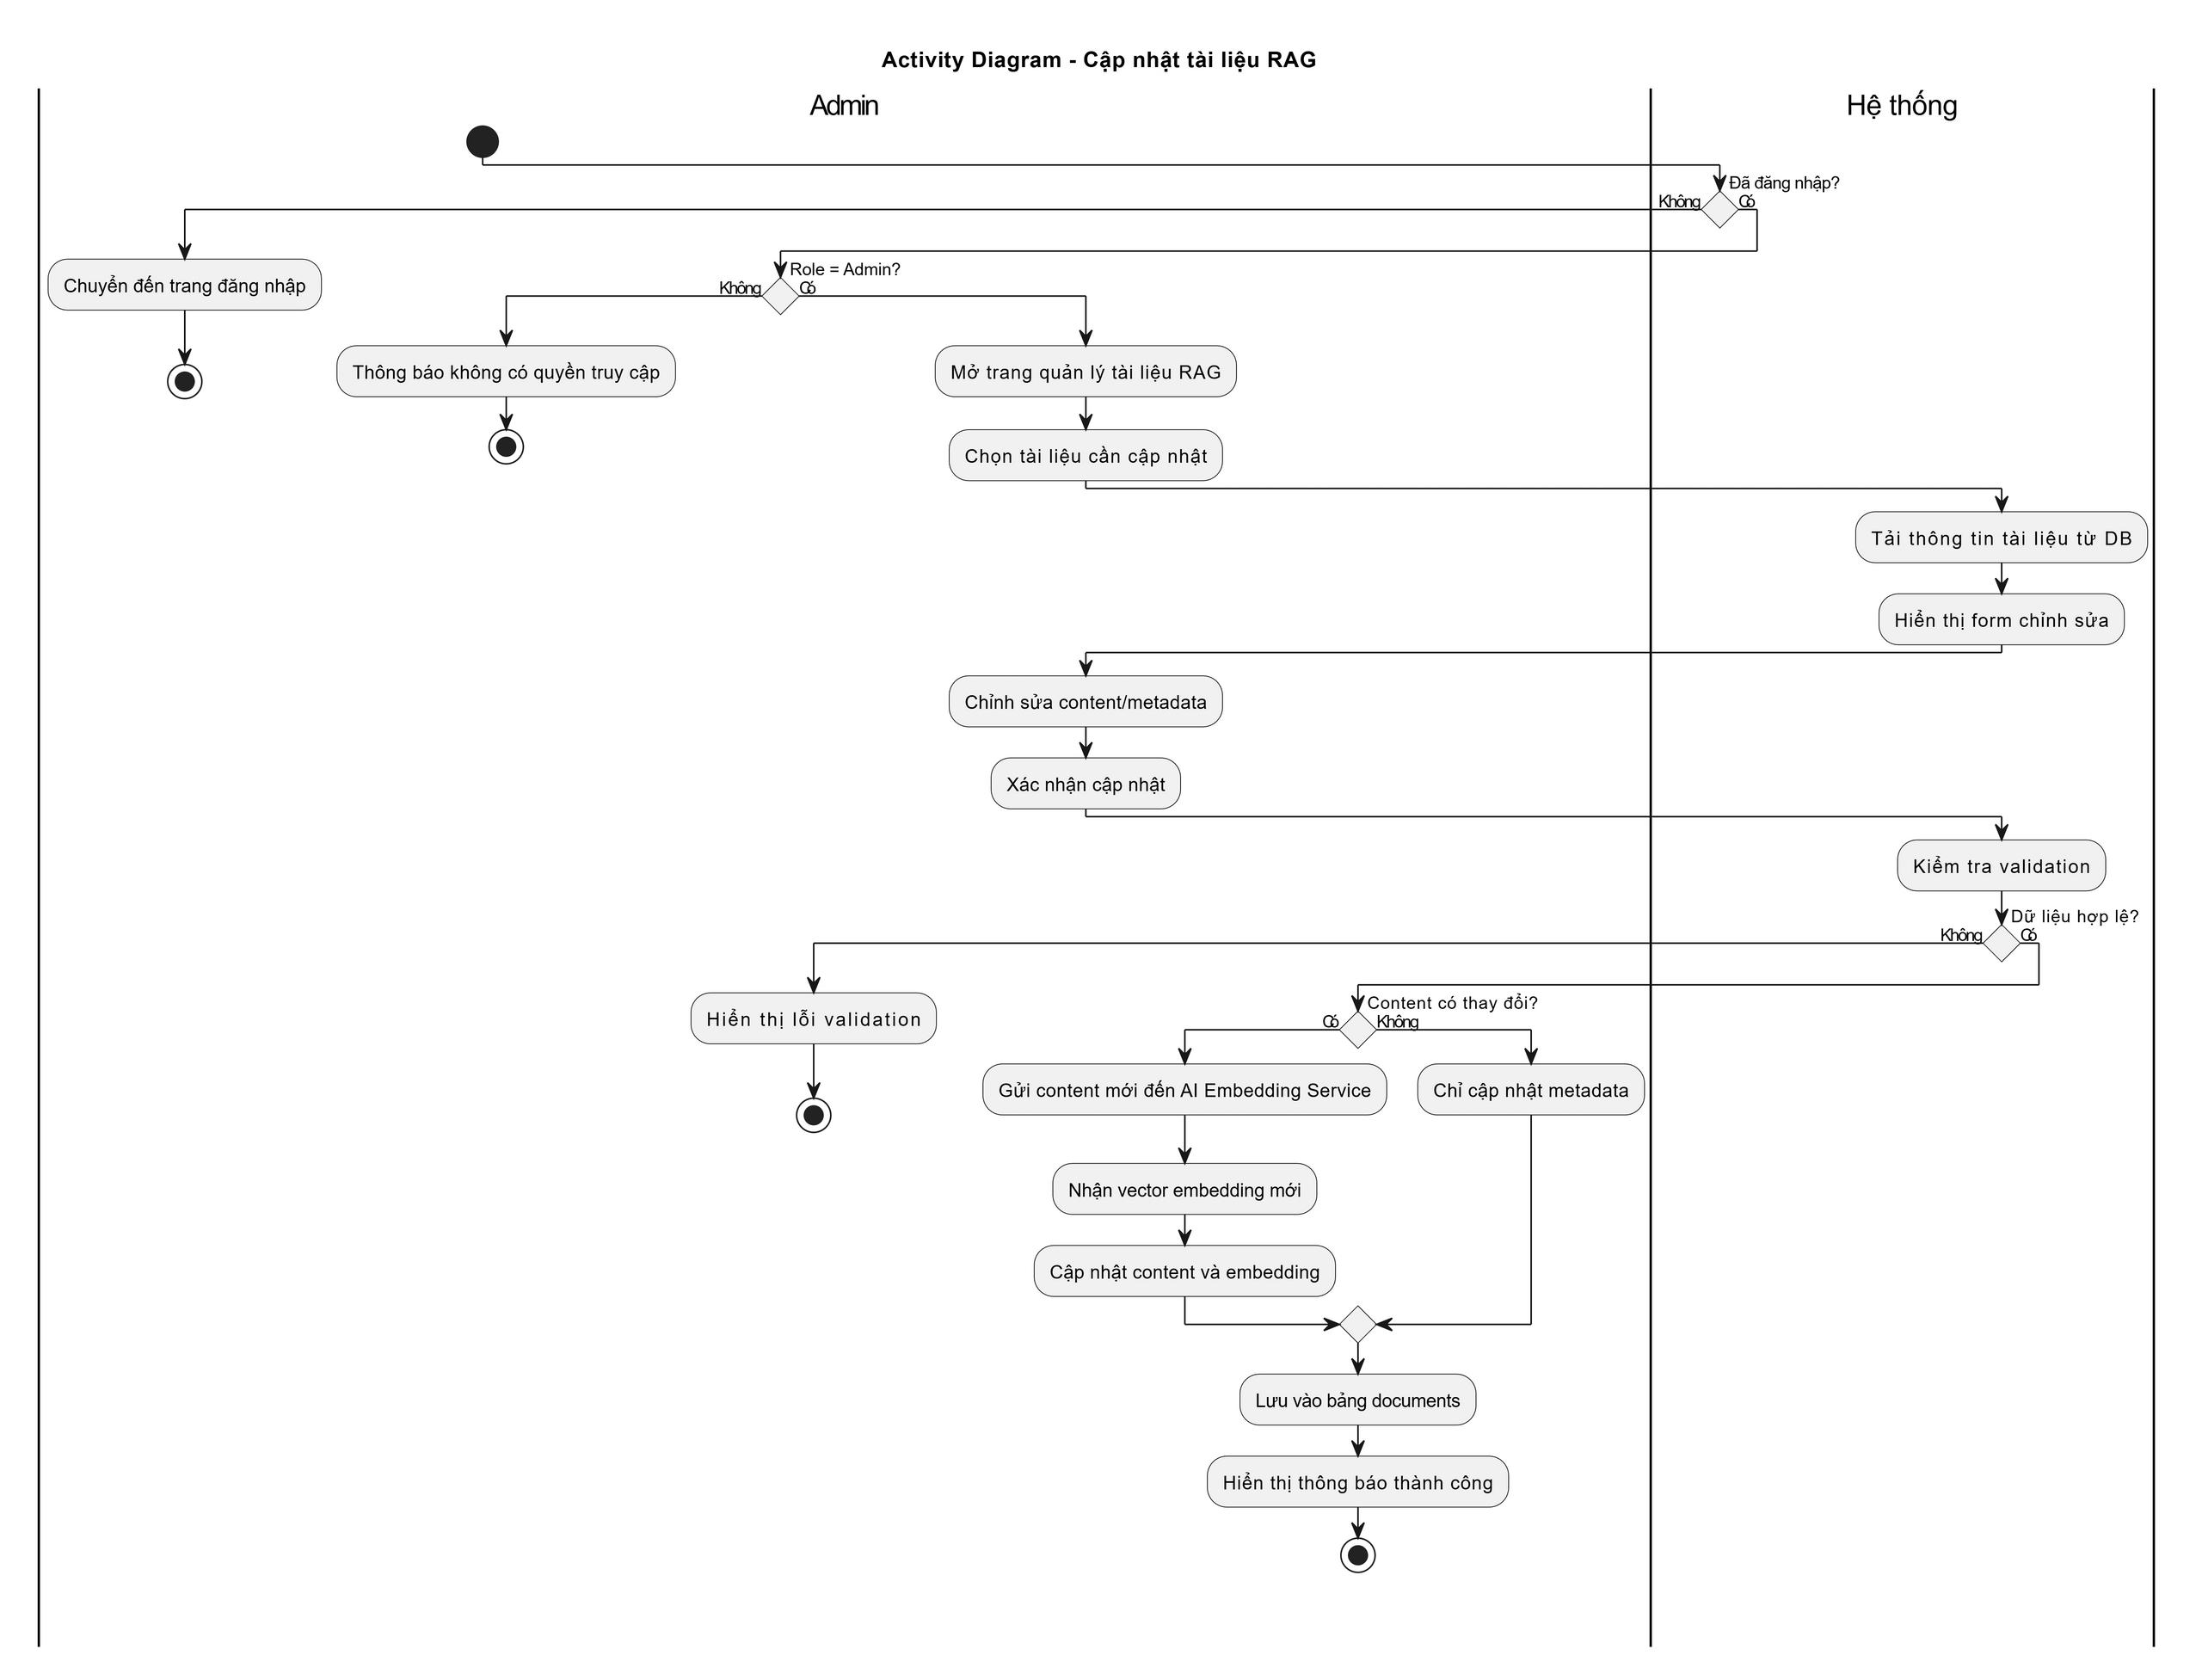
\includegraphics[width=0.8\textwidth]{figures/ac_update_rag.jpg}
    \caption{Activity Diagram cập nhật tài liệu RAG}
    \label{fig:ac_update_rag}
\end{figure}
\textbf{Mục đích:} Cho phép Admin chỉnh sửa và cập nhật thông tin tài liệu trong Vector Database để cải thiện chất lượng tư vấn của chatbot RAG.

\textbf{Luồng hoạt động:}

\begin{itemize}
    \item Hệ thống kiểm tra đăng nhập:
    \begin{itemize}
        \item \textit{Nếu chưa đăng nhập:} Chuyển đến trang đăng nhập và kết thúc.
        \item \textit{Nếu đã đăng nhập:} Kiểm tra quyền truy cập.
    \end{itemize}
    
    \item Hệ thống kiểm tra Role = Admin:
    \begin{itemize}
        \item \textit{Nếu không:} Thông báo không có quyền truy cập và kết thúc.
        \item \textit{Nếu có:} Mở trang quản lý tài liệu RAG.
    \end{itemize}
    
    \item Admin chọn tài liệu cần cập nhật.
    
    \item Hệ thống tải thông tin tài liệu từ DB và hiển thị form chỉnh sửa.
    
    \item Admin chỉnh sửa content/metadata.
    
    \item Admin xác nhận cập nhật.
    
    \item Hệ thống kiểm tra validation:
    \begin{itemize}
        \item \textit{Nếu không hợp lệ:} Hiển thị lỗi validation và kết thúc.
        \item \textit{Nếu hợp lệ:} Kiểm tra content có thay đổi.
    \end{itemize}
    
    \item Hệ thống kiểm tra content có thay đổi:
    \begin{itemize}
        \item \textit{Nếu có:}
        \begin{itemize}
            \item Gửi content mới đến AI Embedding Service
            \item Nhận vector embedding mới
            \item Cập nhật content và embedding
        \end{itemize}
        \item \textit{Nếu không:} Chỉ cập nhật metadata.
    \end{itemize}
    
    \item Lưu vào bảng documents.
    
    \item Hiển thị thông báo thành công.
    
    \item Kết thúc quy trình.
\end{itemize}

\subsection{Activity Diagram xóa tài liệu RAG}
\begin{figure}[H]
    \centering
    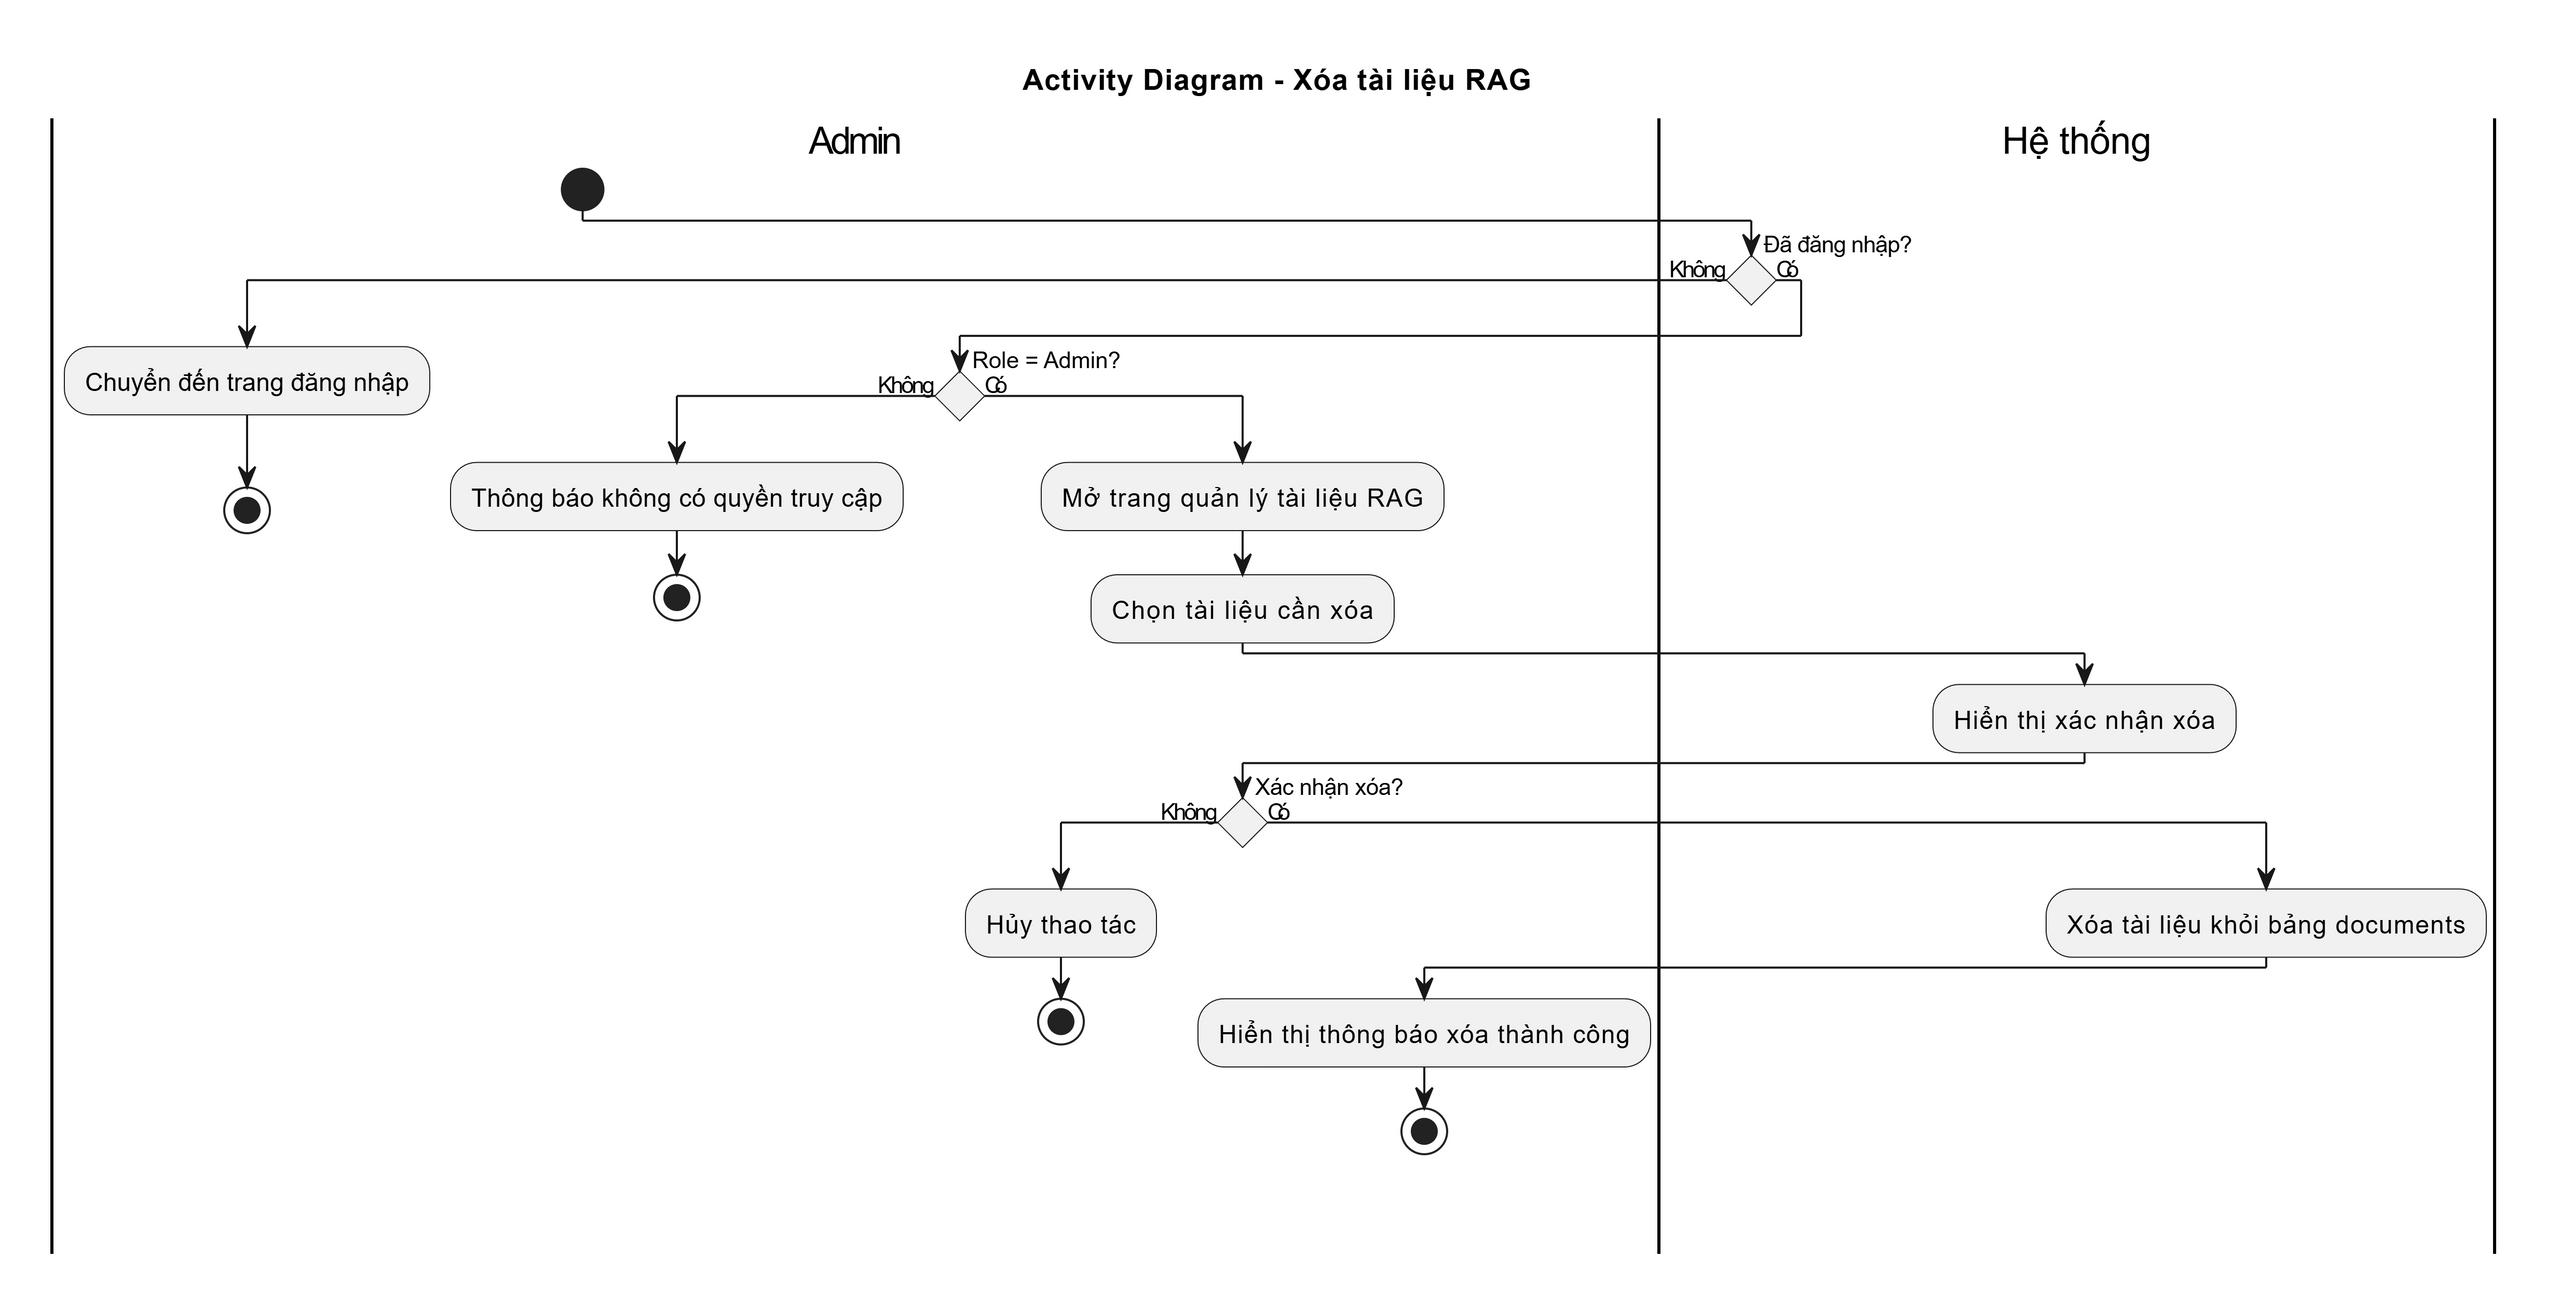
\includegraphics[width=0.8\textwidth]{figures/ac_xoa_rag.jpg}
    \caption{Activity Diagram xóa tài liệu RAG}
    \label{fig:ac_xoa_rag}
\end{figure}
\textbf{Mục đích:} Cho phép Admin xóa tài liệu không còn phù hợp hoặc lỗi thời khỏi Vector Database để duy trì chất lượng dữ liệu cho chatbot RAG.

\textbf{Luồng hoạt động:}

\begin{itemize}
    \item Hệ thống kiểm tra đăng nhập:
    \begin{itemize}
        \item  \textit{Nếu chưa đăng nhập:} Chuyển đến trang đăng nhập và kết thúc.
        \item  \textit{Nếu đã đăng nhập:} Kiểm tra quyền truy cập.
    \end{itemize}
    
    \item Hệ thống kiểm tra Role = Admin:
    \begin{itemize}
        \item  \textit{Nếu không:} Thông báo không có quyền truy cập và kết thúc.
        \item  \textit{Nếu có:} Mở trang quản lý tài liệu RAG.
    \end{itemize}
    
    \item Admin chọn tài liệu cần xóa.
    
    \item Hệ thống hiển thị xác nhận xóa.
    
    \item Admin xác nhận xóa:
    \begin{itemize}
        \item  \textit{Nếu không:} Hủy thao tác và kết thúc.
        \item  \textit{Nếu có:} Xóa tài liệu khỏi bảng documents.
    \end{itemize}
    
    \item Hiển thị thông báo xóa thành công.
    
    \item Kết thúc quy trình.
\end{itemize}

\section{Giao diện người dùng}
\subsection{Giao diện bắt đầu}
\begin{figure}[H]
    \centering
    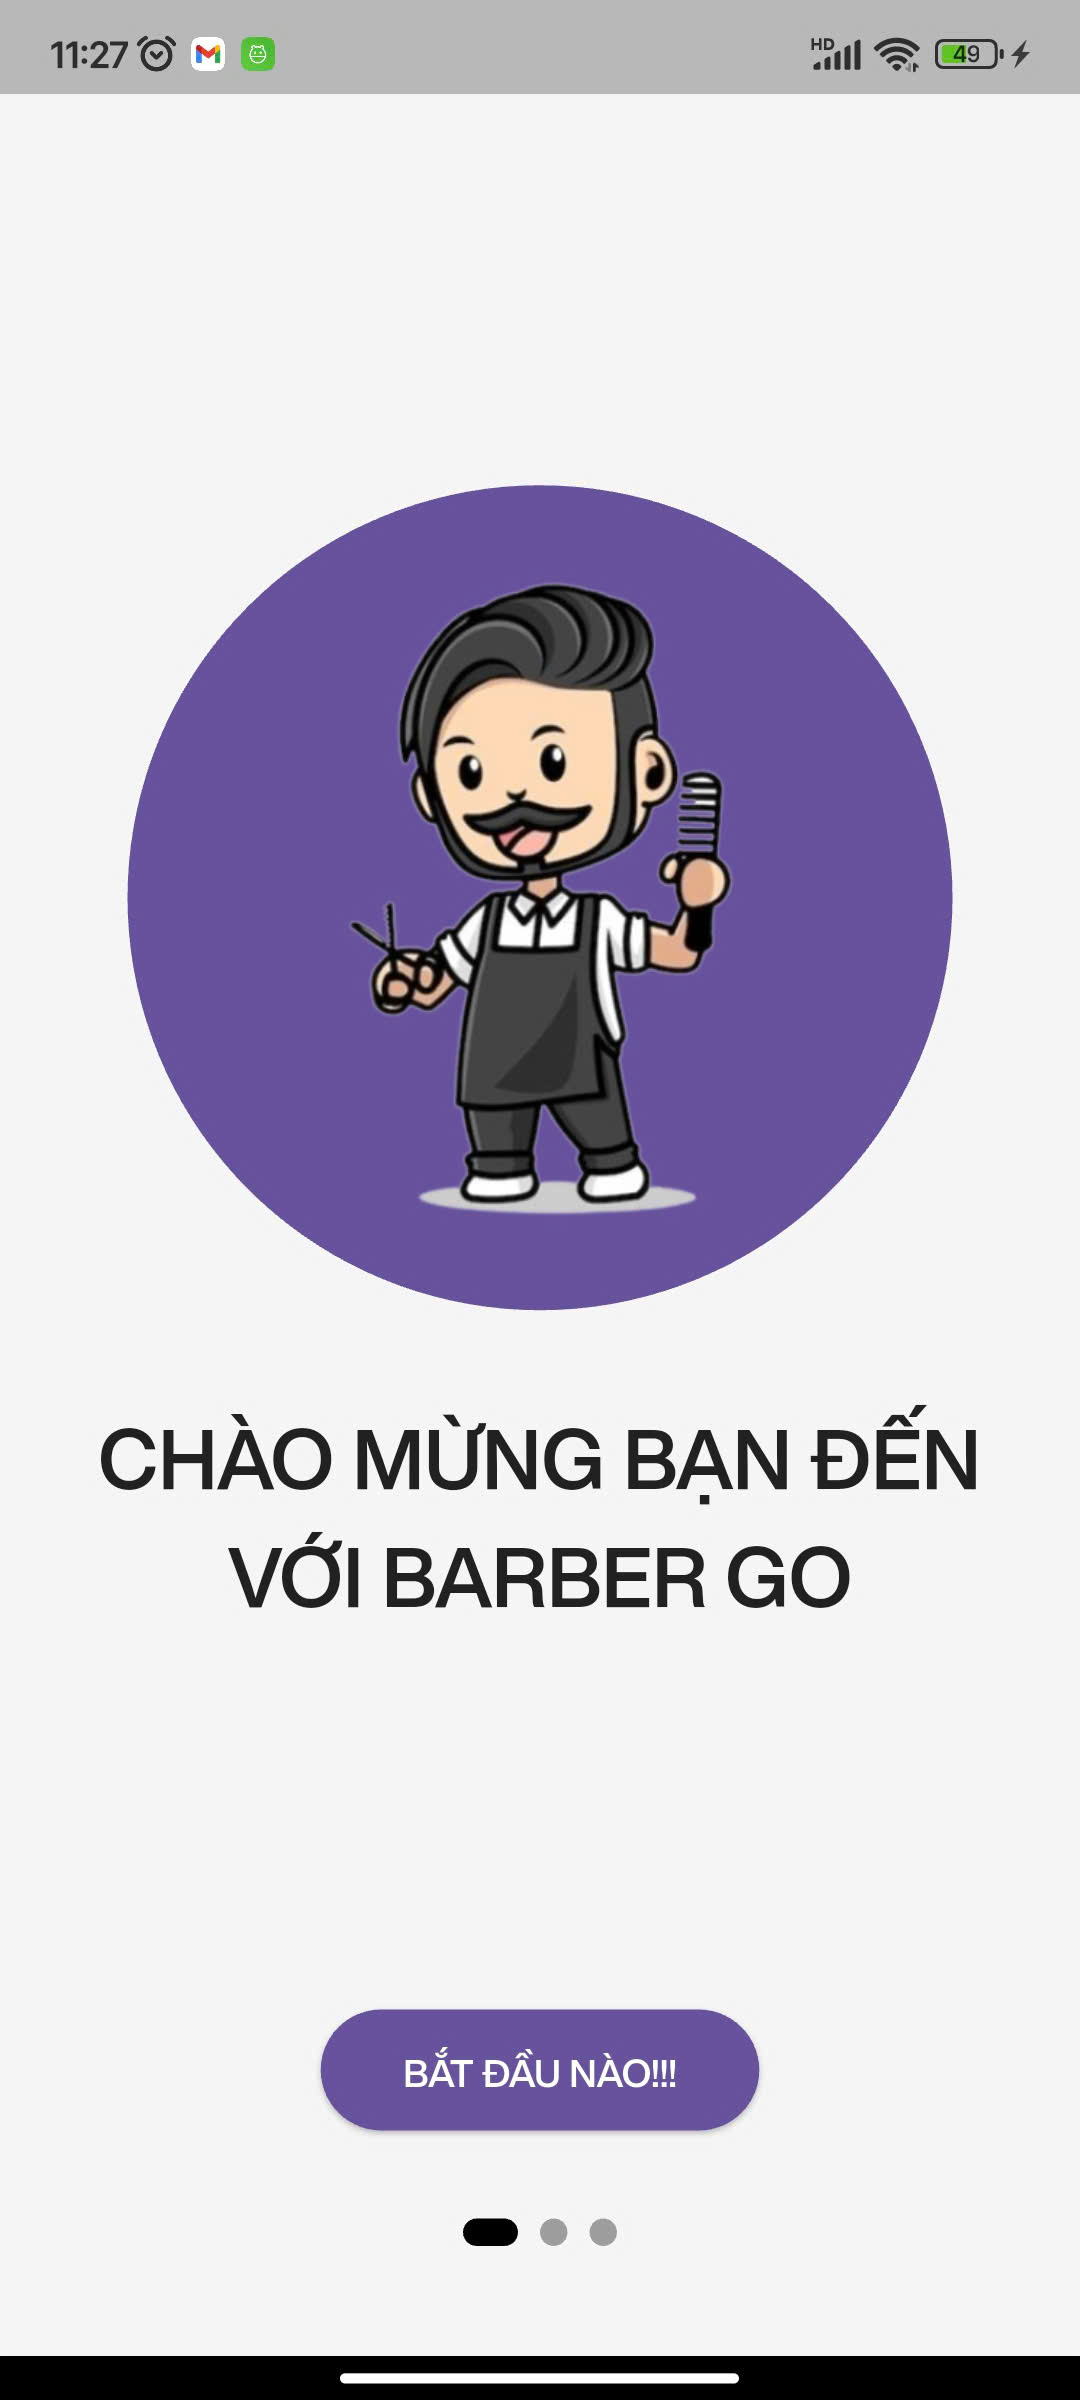
\includegraphics[width=0.5\textwidth]{figures/intro.jpg}
    \caption{Giao diện bắt đầu}
    \label{fig:intro}
\end{figure}



\subsection{Giao diện đăng ký}
\begin{figure}[H]
    \centering
    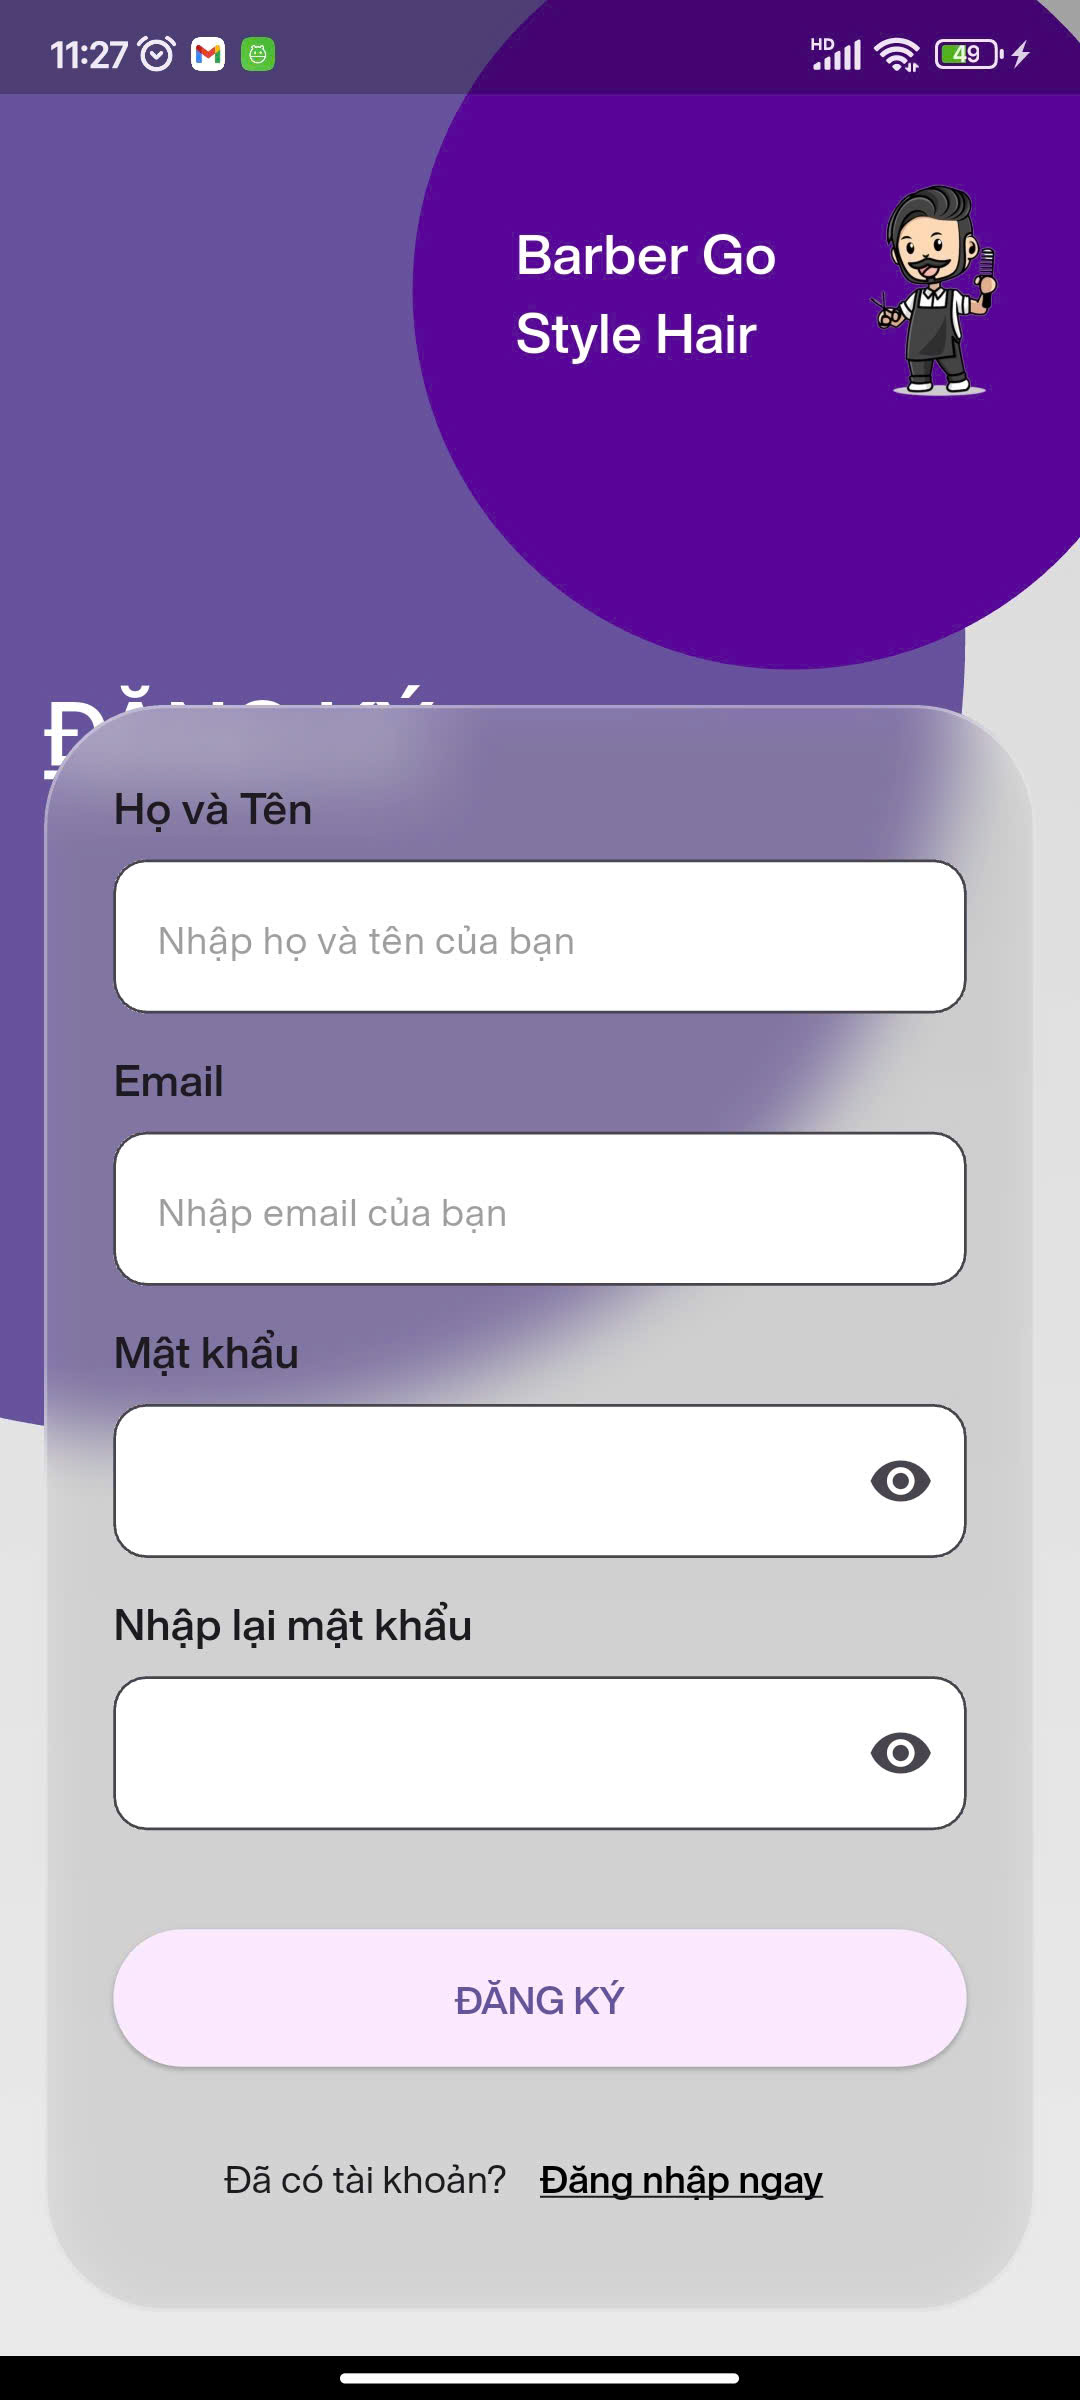
\includegraphics[width=0.5\textwidth]{figures/dk.jpg}
    \caption{Giao diện đăng ký}
    \label{fig:dk}
\end{figure}

\subsection{Giao diện trang chủ}
\begin{figure}[H]
    \centering
    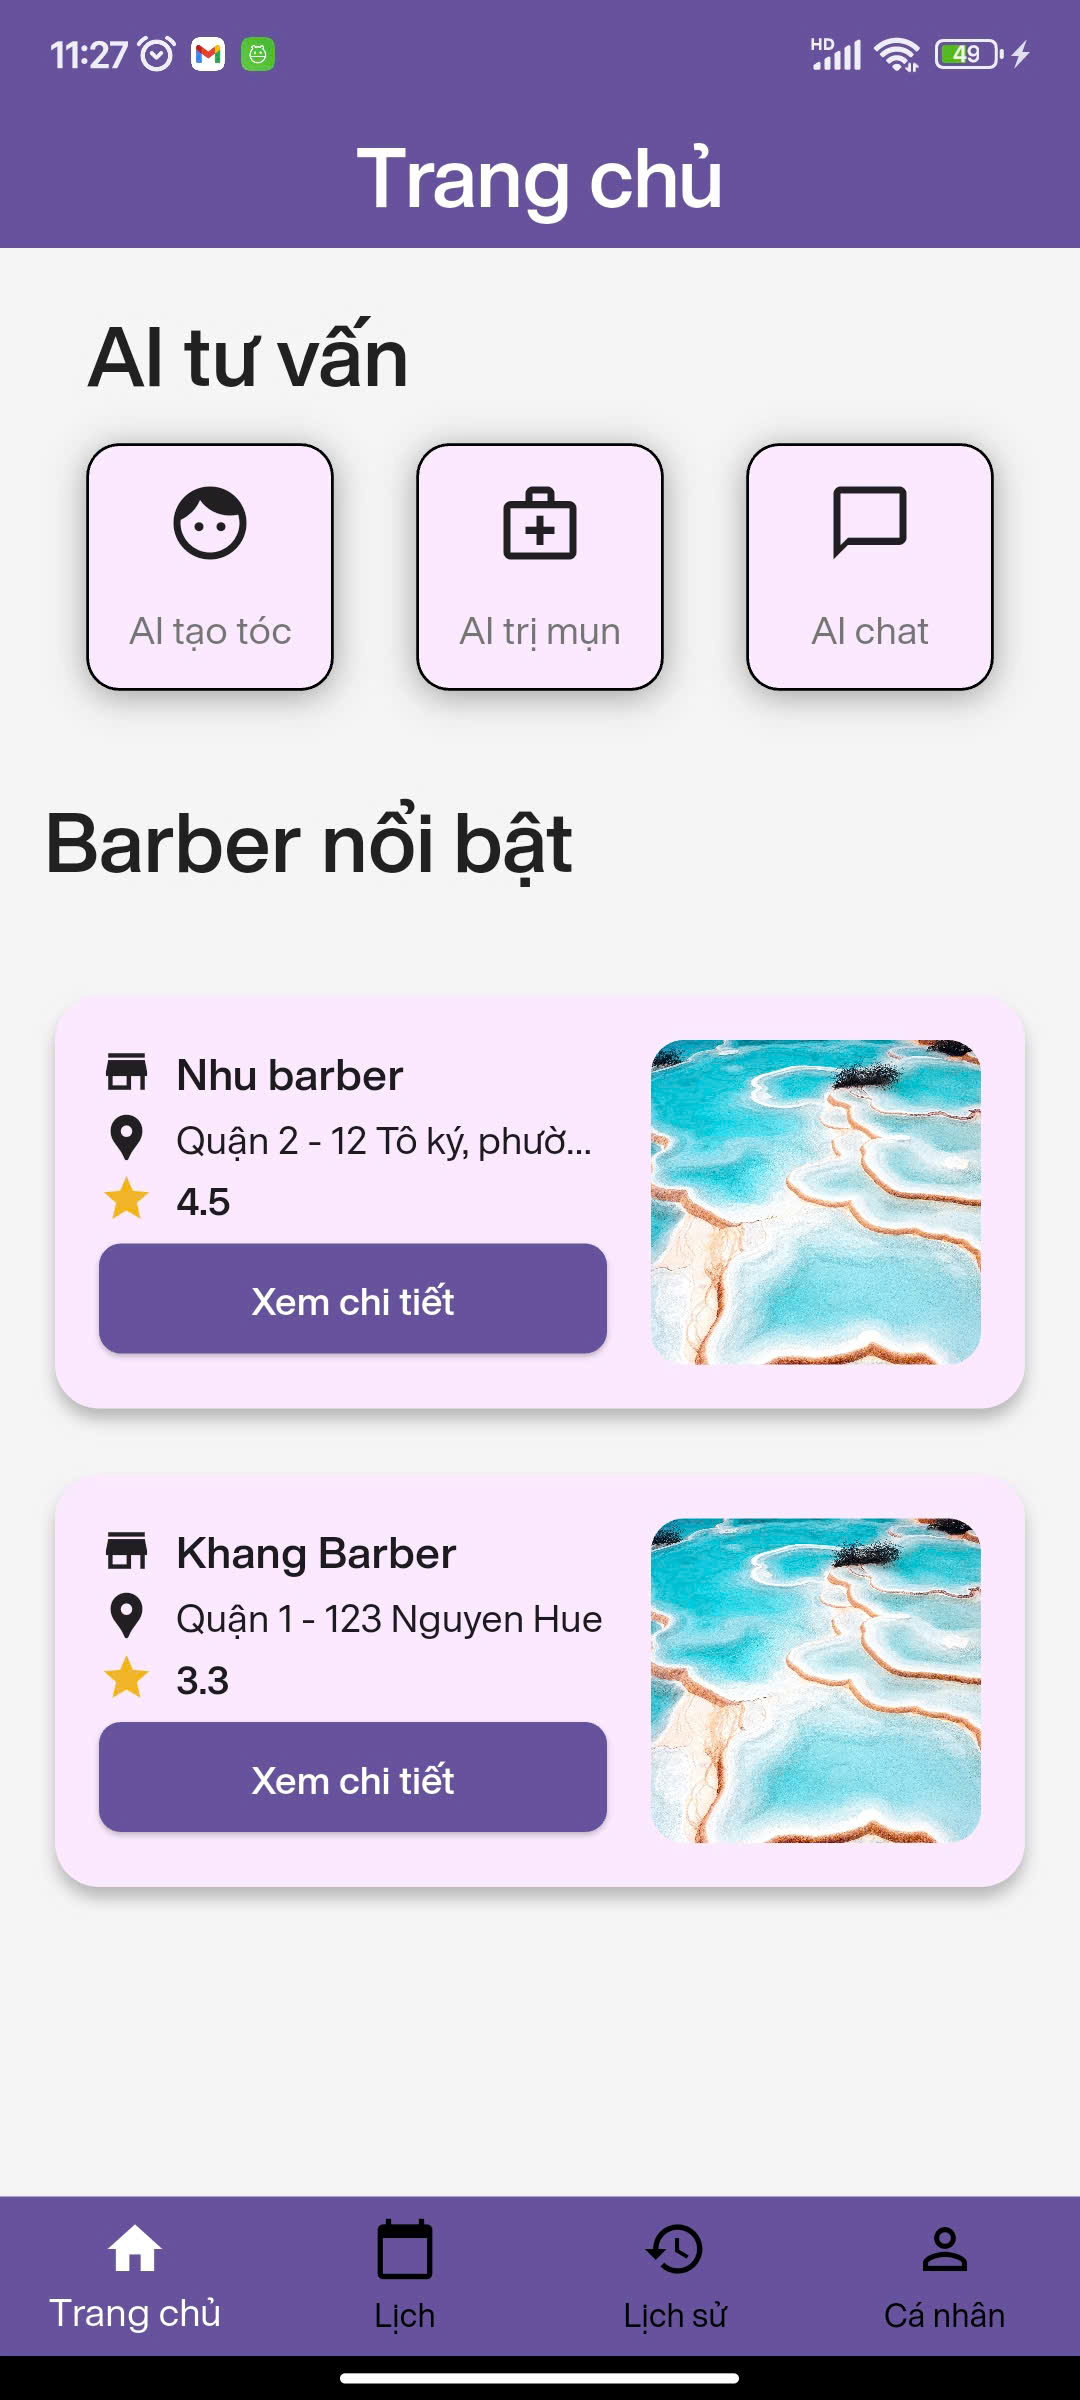
\includegraphics[width=0.5\textwidth]{figures/home.jpg}
    \caption{Giao diện trang chủ}
    \label{fig:home}
\end{figure}


\subsection{Giao diện lịch}
\begin{figure}[H]
    \centering
    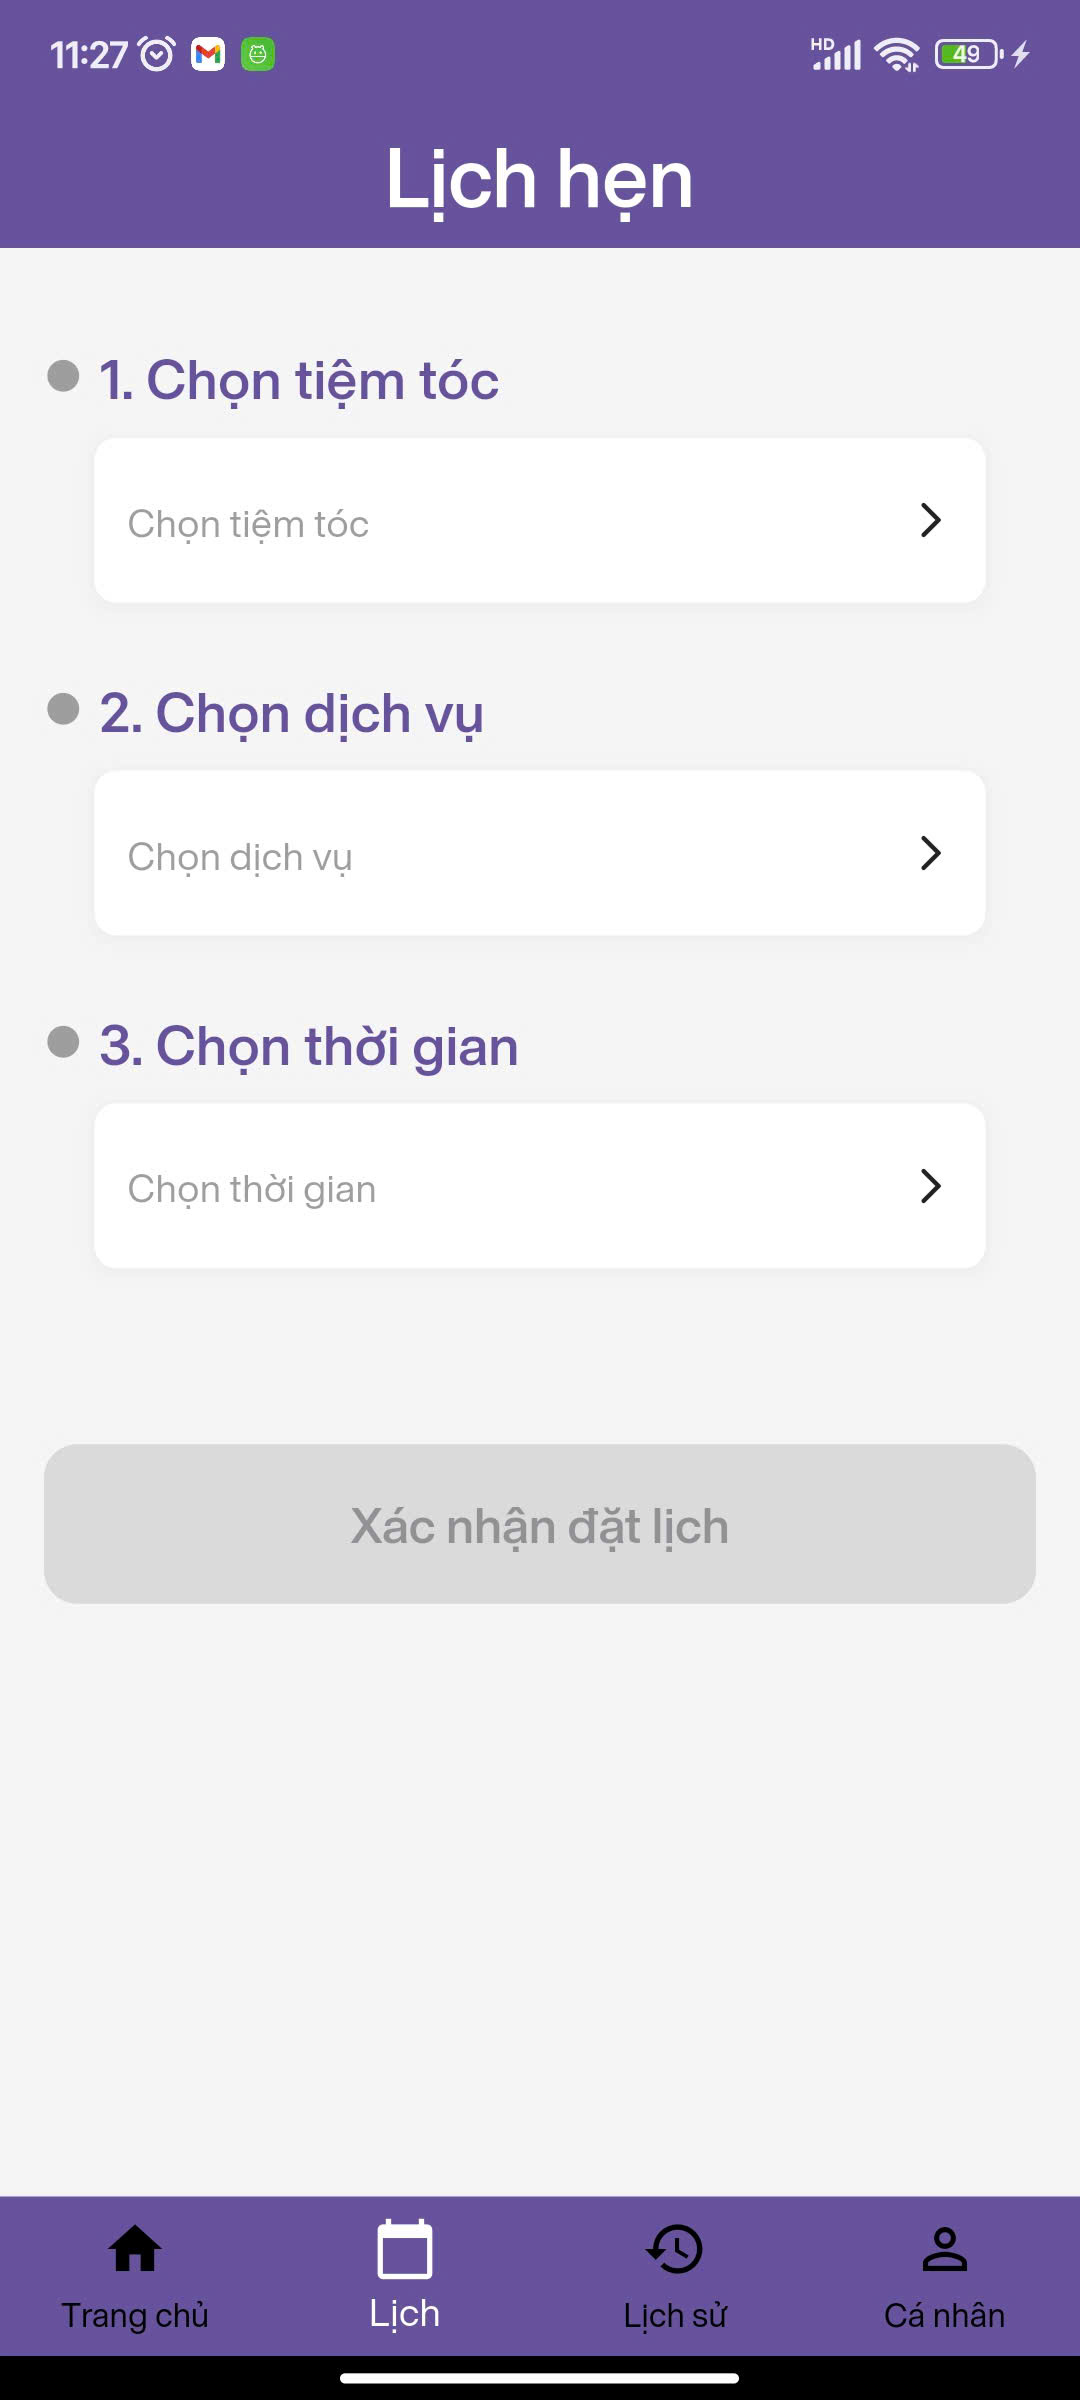
\includegraphics[width=0.5\textwidth]{figures/lich.jpg}
    \caption{Giao diện lịch}
    \label{fig:lich}
\end{figure}


\subsection{Giao diện lịch sử }
\begin{figure}[H]
    \centering
    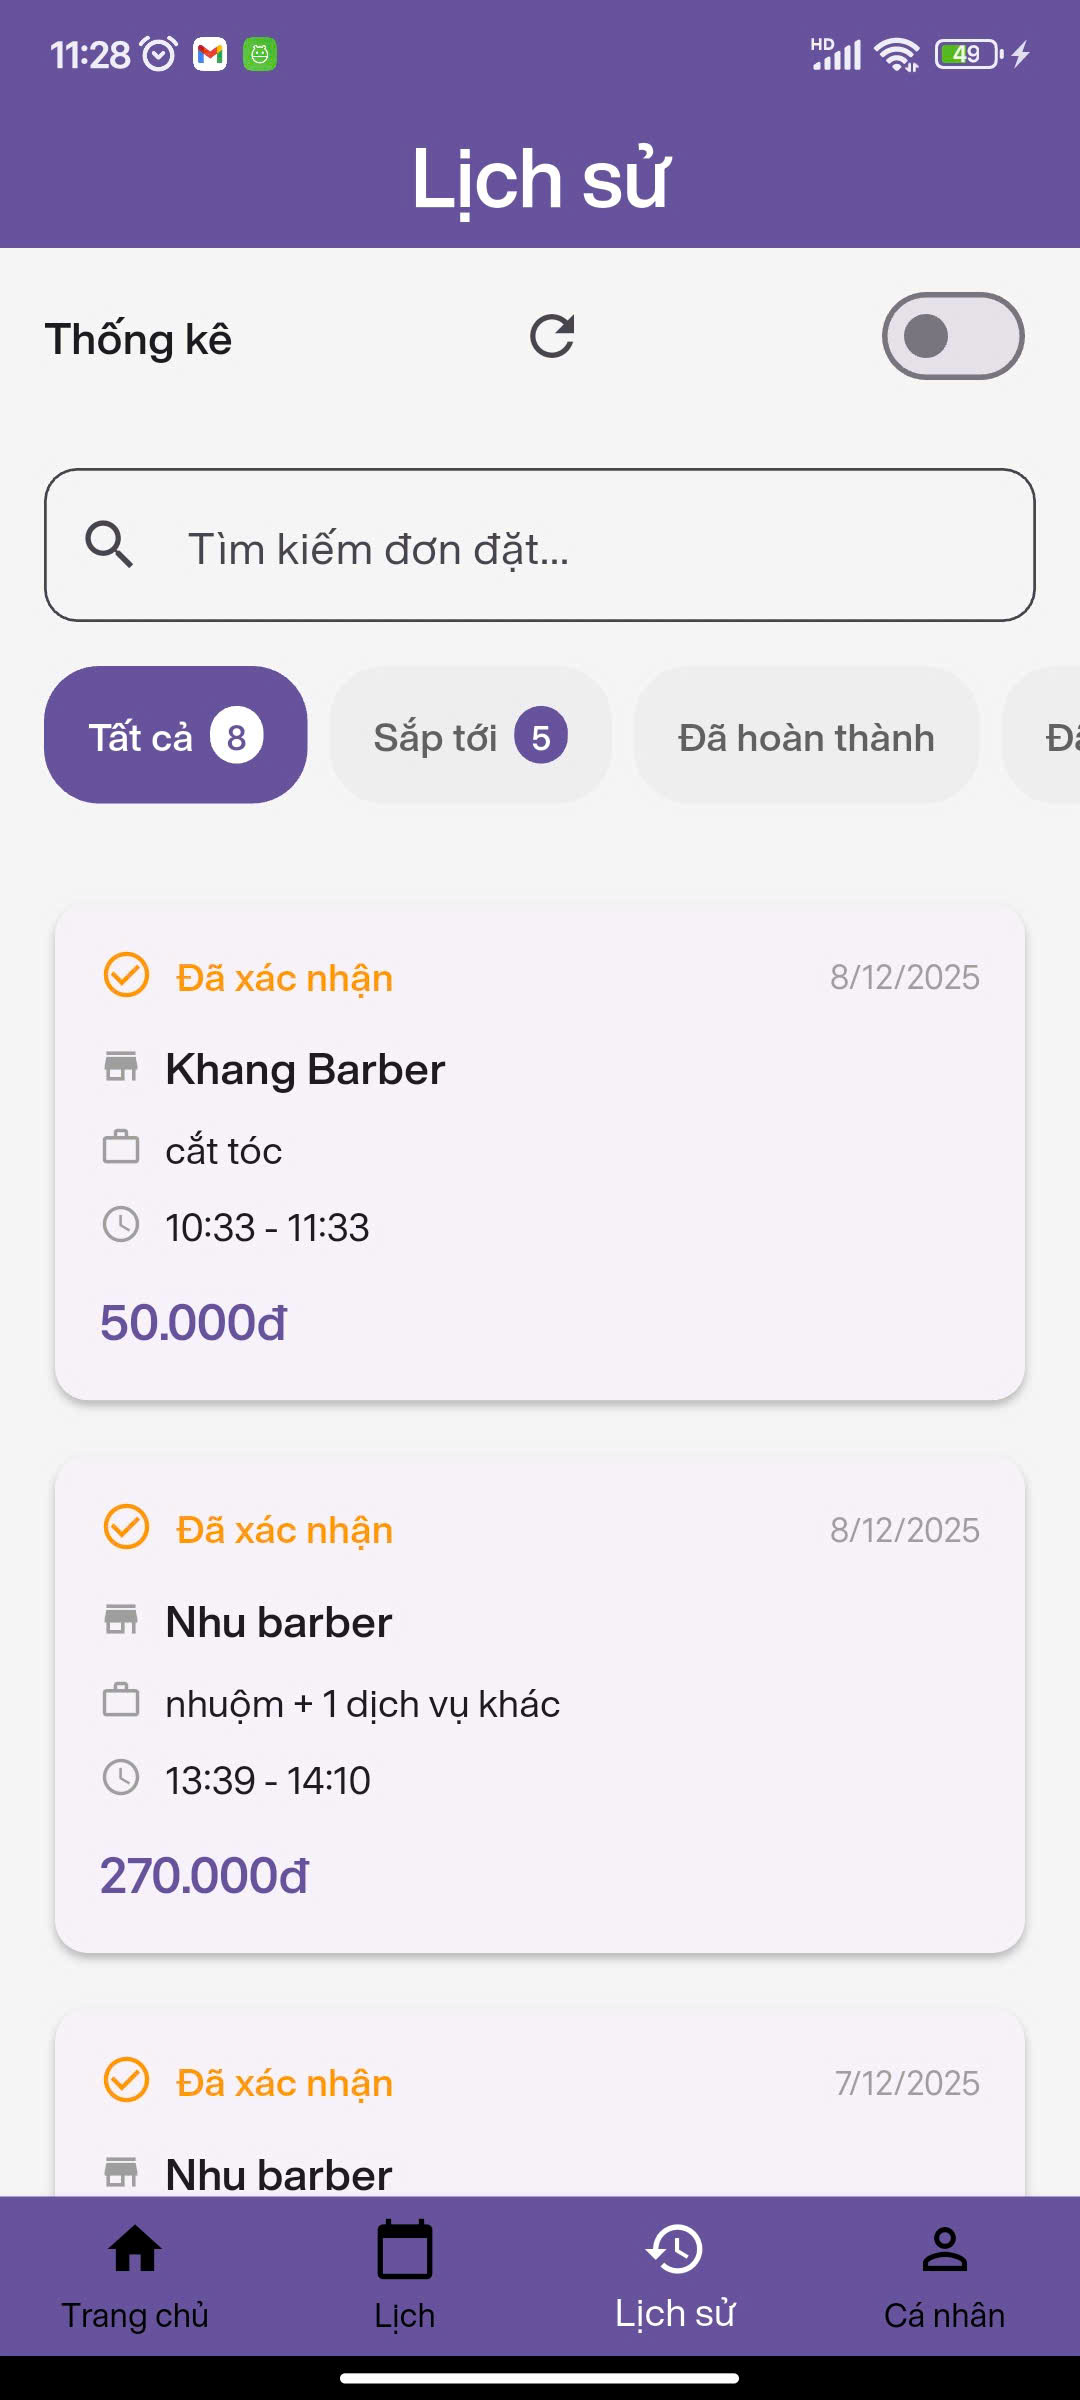
\includegraphics[width=0.5\textwidth]{figures/lich_su.jpg}
    \caption{Giao diện lịch sử}
    \label{fig:lich_su}
\end{figure}

\subsection{Giao diện trang cá nhân}
\begin{figure}[H]
    \centering
    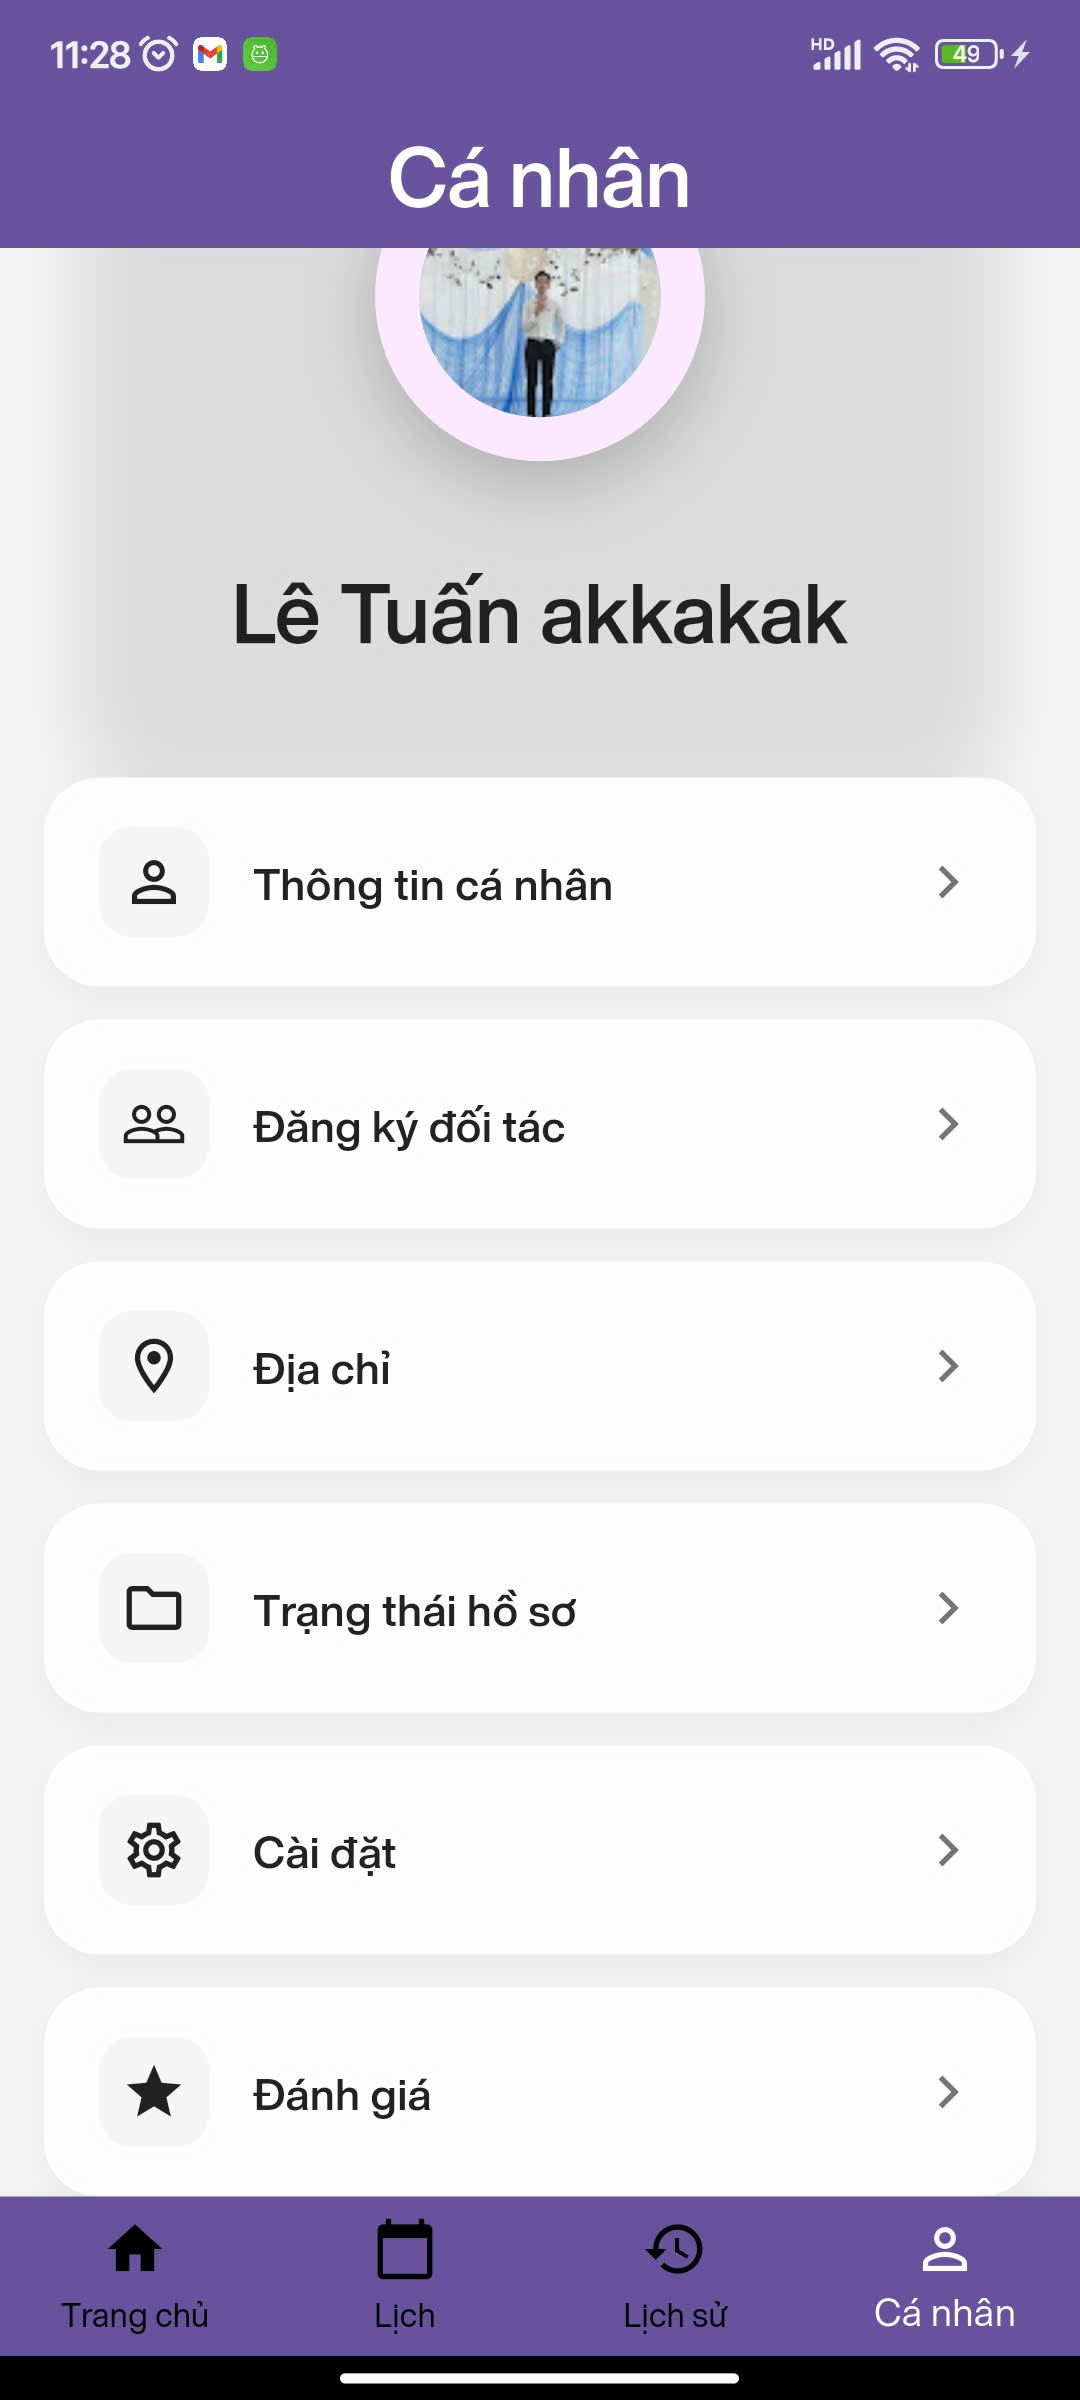
\includegraphics[width=0.5\textwidth]{figures/profile.jpg}
    \caption{Giao diện trang cá nhân}
    \label{fig:profile}
\end{figure}

% 14. chương 4
\chapter{KIỂM THỬ VÀ TRIỂN KHAI HỆ THỐNG}
\section{Kiểm thử hệ thống}

\subsection{Mục tiêu kiểm thử}
Đảm bảo các chức năng chính của hệ thống BarberGo hoạt động chính xác, ổn định và đáp ứng yêu cầu người dùng.

\subsection{Phạm vi kiểm thử}

\subsubsection{Mobile App - Người dùng}
\begin{itemize}
    \item Đặt lịch cắt tóc
    \item Tạo gợi ý kiểu tóc bằng AI Stable Diffusion 1.5
    \item Phát hiện mụn trên khuôn mặt với CNN và Mediapipe
    \item Chatbot tư vấn với RAG
    \item Đăng ký nâng cấp tài khoản chủ tiệm
\end{itemize}

\subsubsection{Mobile App - Chủ tiệm}
\begin{itemize}
    \item Quản lý lịch hẹn và lịch làm việc
    \item Cập nhật thông tin tiệm và dịch vụ
    \item Cập nhật vị trí tiệm trên bản đồ
\end{itemize}

\subsubsection{Web Admin}
\begin{itemize}
    \item Quản lý chủ tiệm và người dùng
    \item Chỉnh sửa prompt chatbot
\end{itemize}

\subsection{Phương pháp kiểm thử}

\begin{table}[H]
\centering
\caption{Phương pháp kiểm thử hệ thống}
\begin{tabular}{|l|p{0.35\textwidth}|l|}
\hline
\textbf{Loại} & \textbf{Mục đích} & \textbf{Công cụ} \\
\hline
Unit Testing & Kiểm thử từng module riêng lẻ & Flutter Test \\
\hline
API Testing & Kiểm thử các endpoint & Postman \\
\hline
Integration Testing & Kiểm thử tích hợp module & Postman \\
\hline
AI Model Testing & Kiểm thử độ chính xác model & Python \\
\hline
\end{tabular}
\end{table}

\subsection{Kiểm thử Model AI phát hiện mụn}

Model CNN được huấn luyện để phát hiện mụn trên khuôn mặt người dùng, kết hợp với Mediapipe để xác định vùng khuôn mặt.

\subsubsection{Thông số huấn luyện}
\begin{itemize}
    \item Mô hình MobileNetV2 (Transfer Learning), ảnh đầu vào 224×224
    \item Tập dữ liệu 4,770 ảnh, chia train/validation
    \item Huấn luyện 50 epochs với AdamW và Binary Cross Entropy
\end{itemize}


\subsubsection{Kết quả huấn luyện}

\begin{table}[H]
\centering
\caption{Kết quả huấn luyện Model CNN theo epoch}
\begin{tabular}{|c|c|c|c|c|}
\hline
\textbf{Epoch} & \textbf{Train Loss} & \textbf{Train Acc} & \textbf{Val Loss} & \textbf{Val Acc} \\
\hline
1 & 0.0784 & 0.9750 & 0.0131 & 0.9953 \\
\hline
5 & 0.0101 & 0.9973 & 0.0007 & 1.0000 \\
\hline
10 & 0.0088 & 0.9973 & 0.0006 & 1.0000 \\
\hline
15 & 0.0020 & 0.9994 & 0.0009 & 1.0000 \\
\hline
20 & 0.0007 & 0.9996 & 0.0001 & 1.0000 \\
\hline
25 & 0.0007 & 0.9997 & 0.0001 & 1.0000 \\
\hline
30 & 0.0008 & 0.9997 & 0.0001 & 1.0000 \\
\hline
35 & 0.0009 & 0.9999 & 0.0000 & 1.0000 \\
\hline
40 & 0.0017 & 0.9997 & 0.0001 & 1.0000 \\
\hline
45 & 0.0017 & 0.9999 & 0.0000 & 1.0000 \\
\hline
50 & 0.0011 & 0.9997 & 0.0001 & 1.0000 \\
\hline
\end{tabular}
\end{table}

\subsection{Biểu đồ kết quả huấn luyện Model CNN}
\begin{figure}[H]
    \centering
    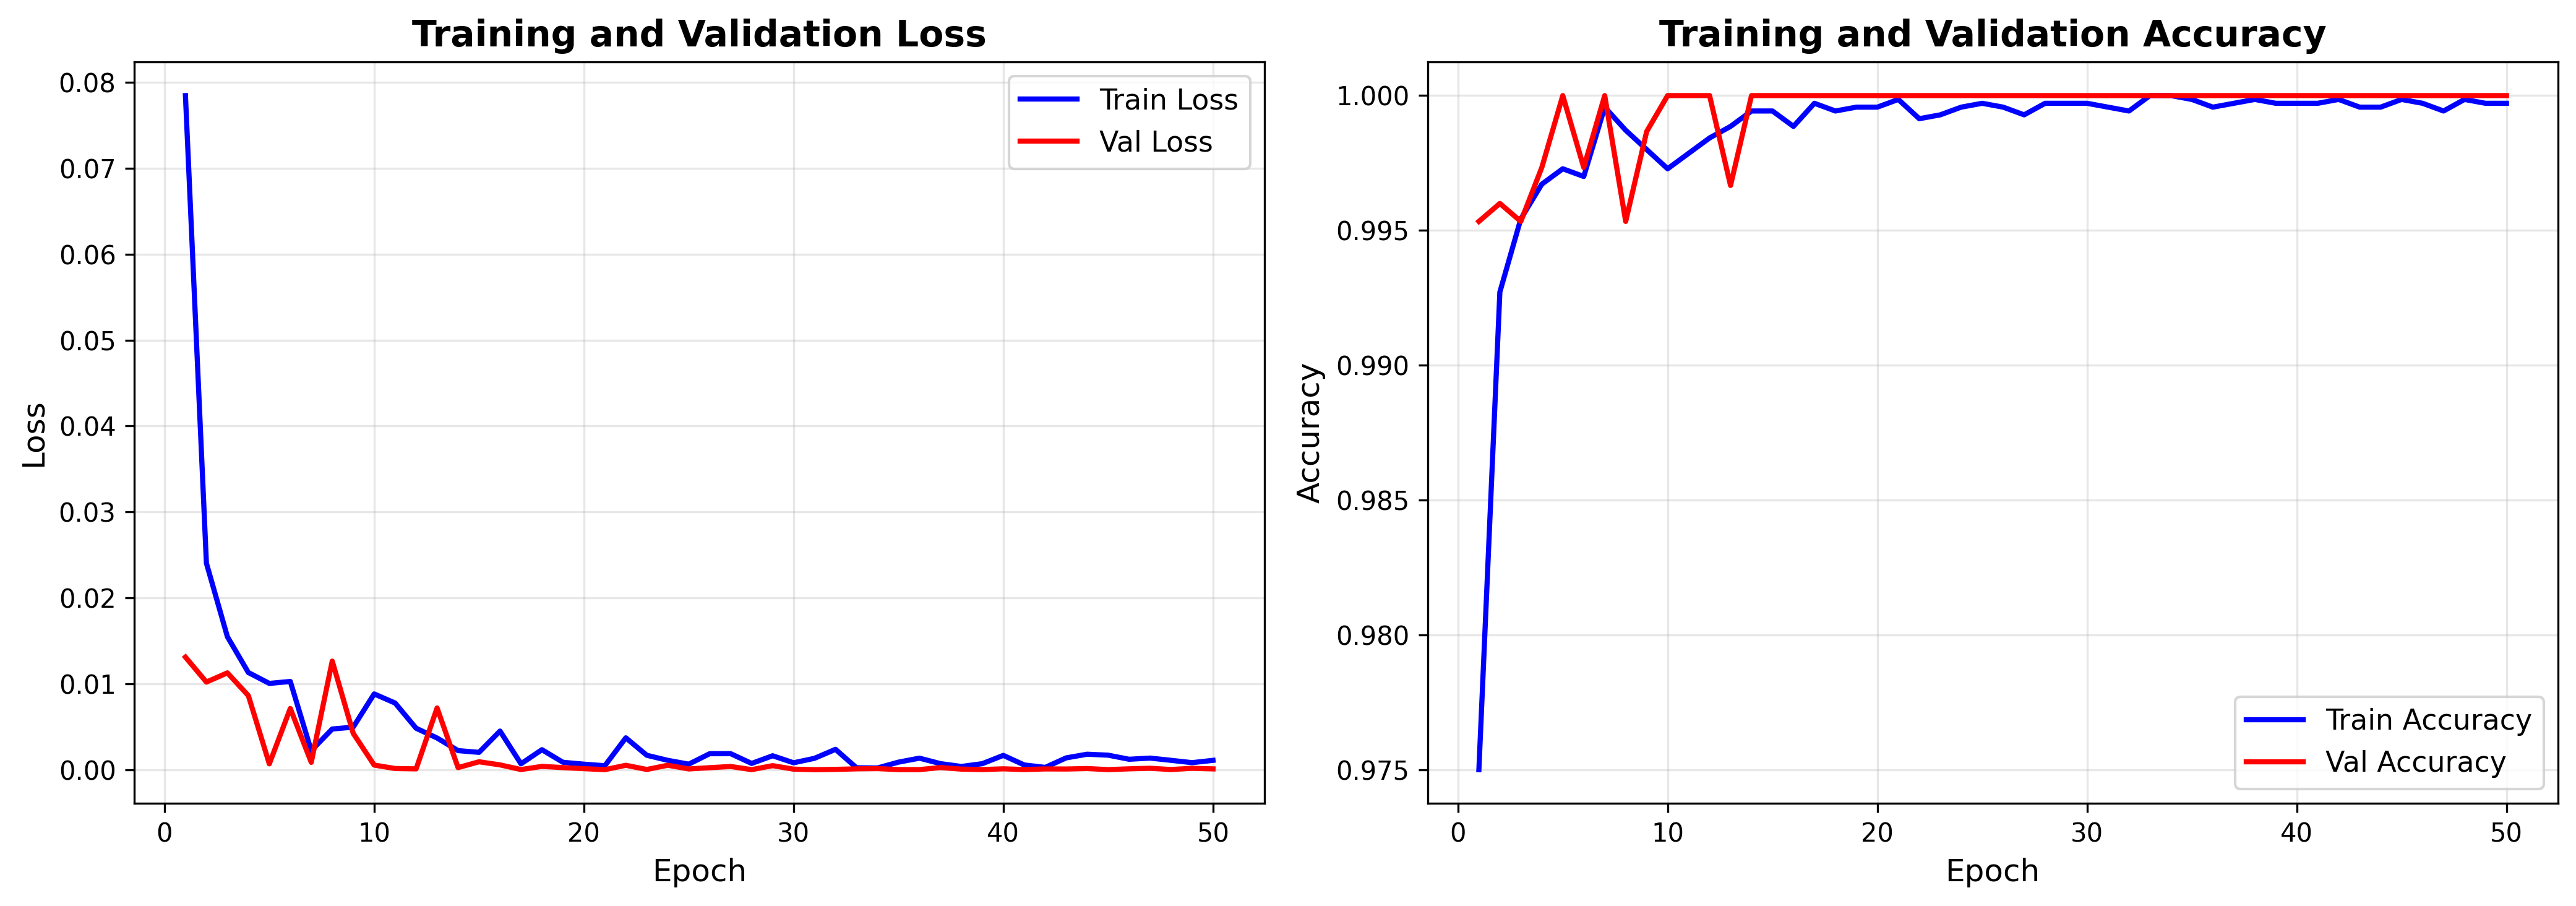
\includegraphics[width=1.0\textwidth]{figures/training_chart.png}
    \caption{Biểu đồ kết quả huấn luyện Model CNN}
    \label{fig:training_chart}
\end{figure}
\subsubsection{Đánh giá kết quả}

Từ kết quả huấn luyện, model đạt được:
\begin{itemize}
    \item Độ chính xác trên tập validation: 100\% (từ epoch 5 trở đi)
    \item Loss giảm nhanh và ổn định sau epoch 20
    \item Không có dấu hiệu overfitting nghiêm trọng
    \item Thời gian inference: dưới 3 giây
\end{itemize}

Model cho thấy khả năng phân loại tốt giữa ảnh có mụn và không có mụn, phù hợp để tích hợp vào ứng dụng thực tế.

\subsection{Kiểm thử API}

\subsubsection{Danh sách Endpoints}

Hệ thống BarberGo cung cấp các nhóm API sau:

\textbf{Authentication APIs}
\begin{itemize}
    \item POST /api/auth/register - Đăng ký tài khoản
    \item POST /api/auth/login - Đăng nhập
    \item POST /api/auth/logout - Đăng xuất
    \item POST /api/auth/refresh-token - Làm mới token
\end{itemize}

\textbf{User APIs}
\begin{itemize}
    \item GET /api/users/profile - Xem thông tin cá nhân
    \item PUT /api/users/profile - Cập nhật thông tin
    \item POST /api/users/upgrade-to-owner - Nâng cấp chủ tiệm
    \item GET /api/users/bookings - Xem lịch hẹn
\end{itemize}

\textbf{Booking APIs}
\begin{itemize}
    \item GET /api/bookings - Danh sách lịch hẹn
    \item POST /api/bookings - Tạo lịch hẹn
    \item GET /api/bookings/\{id\} - Chi tiết lịch hẹn
    \item PUT /api/bookings/\{id\} - Cập nhật lịch hẹn
    \item DELETE /api/bookings/\{id\} - Hủy lịch hẹn
\end{itemize}

\textbf{Shop APIs}
\begin{itemize}
    \item GET /api/shops - Danh sách tiệm
    \item GET /api/shops/\{id\} - Chi tiết tiệm
    \item POST /api/shops - Tạo tiệm mới
    \item PUT /api/shops/\{id\} - Cập nhật thông tin tiệm
    \item PUT /api/shops/\{id\}/location - Cập nhật vị trí
    \item GET /api/shops/\{id\}/services - Danh sách dịch vụ
    \item POST /api/shops/\{id\}/services - Thêm dịch vụ
\end{itemize}

\textbf{Schedule APIs}
\begin{itemize}
    \item GET /api/schedules - Xem lịch làm việc
    \item POST /api/schedules - Tạo lịch làm việc
    \item PUT /api/schedules/\{id\} - Cập nhật lịch
    \item DELETE /api/schedules/\{id\} - Xóa lịch
\end{itemize}

\textbf{AI APIs}
\begin{itemize}
    \item POST /api/ai/hairstyle-generate - Tạo gợi ý kiểu tóc
    \item POST /api/ai/acne-detection - Phát hiện mụn
    \item GET /api/ai/results/\{id\} - Lấy kết quả AI
\end{itemize}

\textbf{Chatbot APIs}
\begin{itemize}
    \item POST /api/chatbot/message - Gửi tin nhắn
    \item GET /api/chatbot/history - Lịch sử chat
    \item DELETE /api/chatbot/history - Xóa lịch sử
\end{itemize}

\textbf{Admin APIs}
\begin{itemize}
    \item GET /api/admin/users - Danh sách người dùng
    \item PUT /api/admin/users/\{id\}/status - Cập nhật trạng thái
    \item DELETE /api/admin/users/\{id\} - Xóa người dùng
    \item GET /api/admin/shops - Danh sách tiệm
    \item PUT /api/admin/shops/\{id\}/approve - Phê duyệt tiệm
    \item PUT /api/admin/chatbot/prompt - Cập nhật prompt
\end{itemize}

\subsubsection{Kết quả kiểm thử API}

\begin{table}[h]
\centering
\caption{Kết quả kiểm thử theo nhóm API}
\begin{tabular}{|l|c|c|}
\hline
\textbf{Nhóm API} & \textbf{Số test} & \textbf{Pass rate} \\
\hline
Authentication & 6 & 100\% \\
\hline
User Management & 8 & 100\% \\
\hline
Booking & 10 & 100\% \\
\hline
Shop & 12 & 92\% \\
\hline
AI Services & 6 & 100\% \\
\hline
Chatbot & 4 & 100\% \\
\hline
Admin & 4 & 100\% \\
\hline
\textbf{Tổng} & \textbf{50} & \textbf{96\%} \\
\hline
\end{tabular}
\end{table}

\subsubsection{Tiêu chí đánh giá}

\begin{table}[h]
\centering
\caption{Tiêu chí đánh giá hiệu năng API}
\begin{tabular}{|l|c|}
\hline
\textbf{Tiêu chí} & \textbf{Mục tiêu} \\
\hline
Tỷ lệ test Pass & $\geq$ 95\% \\
\hline
Response time (API thường) & $\leq$ 2s \\
\hline
Response time (AI Gen ảnh) & $\leq$ 10s \\
\hline
Response time (AI Phát hiện mụn) & $\leq$ 3s \\
\hline
Response time (Chatbot) & $\leq$ 2s \\
\hline
Độ chính xác Model CNN & $\geq$ 95\% \\
\hline
\end{tabular}
\end{table}

\subsection{Môi trường kiểm thử}
\begin{itemize}
    \item Mobile: Flutter 3.x (Android 10+, iOS 14+)
    \item Backend: Python Flask
    \item Web Admin: Nuxt.js 3.x
    \item Database: Supabase PostgreSQL
    \item AI Models: Stable Diffusion 1.5, MobileNetV2, Mediapipe
    \item Tools: Postman, Python
\end{itemize}

\subsection{Kết quả kiểm thử tổng hợp}

Kết quả kiểm thử cho thấy:
\begin{itemize}
    \item Tổng số test cases: 50
    \item Test Pass: 48 (96\%)
    \item Thời gian response trung bình: 1.2 giây
    \item Model CNN đạt 100\% accuracy trên tập validation
    \item Hệ thống hoạt động ổn định và đáp ứng yêu cầu
\end{itemize}


\section{Cài đặt và Triển khai}


\subsection{Môi trường triển khai}

Hệ thống BarberGo được triển khai theo mô hình client-server, bao gồm Backend API, Web Admin và Mobile App. Môi trường triển khai được tóm tắt trong Bảng~\ref{tab:environment}.

\begin{table}[H]
\centering
\caption{Môi trường triển khai hệ thống}
\label{tab:environment}
\begin{tabular}{|p{4cm}|p{9.5cm}|}
\hline
\textbf{Thành phần} & \textbf{Mô tả} \\
\hline
Server &
Ubuntu 22.04 LTS, CPU từ 4 cores, RAM 8GB (khuyến nghị 16GB), SSD 50GB, GPU NVIDIA hỗ trợ CUDA cho AI inference \\
\hline
Backend &
Flask API (Python 3.10+), triển khai với Gunicorn và Nginx \\
\hline
Web Admin &
Ứng dụng web quản trị, build và deploy trên nền tảng CDN (Vercel/Netlify) \\
\hline
Mobile App &
Ứng dụng Flutter, hỗ trợ Android và iOS \\
\hline
Database &
Supabase PostgreSQL, áp dụng Row Level Security (RLS) \\
\hline
AI Models &
Stable Diffusion 1.5 và mô hình CNN phát hiện mụn \\
\hline
\end{tabular}
\end{table}

\subsection{Triển khai hệ thống}

Backend API được triển khai trên server sử dụng Nginx làm reverse proxy nhằm tăng cường khả năng bảo mật và xử lý đồng thời. Các AI models được load khi hệ thống khởi động để phục vụ inference theo yêu cầu.

Web Admin được build thành static files và triển khai trên nền tảng CDN nhằm tối ưu tốc độ truy cập. Mobile App được build bản release và phân phối thông qua Google Play Store và Apple App Store.

\subsection{Bảo mật và vận hành}

Hệ thống áp dụng các biện pháp bảo mật bao gồm HTTPS với SSL/TLS, xác thực người dùng bằng JWT, giới hạn tần suất truy cập API và cấu hình firewall. Cơ chế backup và monitoring được thiết lập nhằm đảm bảo khả năng phục hồi và giám sát trạng thái hệ thống.


\section{Kiểm thử hệ thống}

\subsection{Mục tiêu kiểm thử}

Quá trình kiểm thử nhằm đánh giá tính đúng đắn, ổn định và khả năng hoạt động đồng bộ của các thành phần trong hệ thống BarberGo sau khi triển khai.

\subsection{Kiểm thử chức năng}

Các chức năng chính của hệ thống được kiểm thử bao gồm xác thực người dùng, quản lý lịch hẹn, kết nối cơ sở dữ liệu, xử lý AI và giao tiếp giữa Mobile App, Web Admin với Backend API.

\subsection{Kiểm thử sau triển khai}

Kết quả kiểm thử tổng hợp được trình bày trong Bảng~\ref{tab:testing}.

\begin{table}[H]
\centering
\caption{Kết quả kiểm thử sau triển khai}
\label{tab:testing}
\begin{tabular}{|p{8cm}|c|}
\hline
\textbf{Hạng mục kiểm thử} & \textbf{Kết quả} \\
\hline
Backend API hoạt động ổn định & Đạt \\
\hline
Kết nối cơ sở dữ liệu Supabase & Đạt \\
\hline
AI models load và inference & Đạt \\
\hline
Web Admin kết nối Backend & Đạt \\
\hline
Mobile App giao tiếp API & Đạt \\
\hline
Bảo mật SSL/TLS & Đạt \\
\hline
Logging và monitoring & Đạt \\
\hline
\end{tabular}
\end{table}

\subsection{Đánh giá}

Kết quả kiểm thử cho thấy hệ thống BarberGo đáp ứng đầy đủ các yêu cầu chức năng và phi chức năng đã đề ra. Hệ thống hoạt động ổn định, đảm bảo tính bảo mật và sẵn sàng cho môi trường production.

% 15. chương 5
\chapter{KẾT QUẢ VÀ HƯỚNG PHÁT TRIỂN}

\section{Tổng quan kết quả đạt được}

Sau quá trình phân tích, thiết kế và triển khai, đề tài đã xây dựng thành công hệ thống BarberGo – một hệ thống đặt lịch và quản lý tiệm cắt tóc tích hợp AI. Hệ thống được phát triển theo kiến trúc client--server, đảm bảo khả năng mở rộng, tính ổn định và phù hợp với các ứng dụng thực tế.

Các thành phần chính của hệ thống bao gồm ứng dụng di động cho khách hàng, ứng dụng dành cho chủ tiệm, hệ thống quản trị web và các mô-đun AI. Trong đó, mô hình RAG đóng vai trò trọng tâm, giúp nâng cao chất lượng tương tác giữa người dùng và hệ thống thông qua khả năng truy xuất dữ liệu private để hỗ trợ quá trình tạo sinh câu trả lời.

Kết quả triển khai cho thấy hệ thống đáp ứng đầy đủ các yêu cầu chức năng đã đề ra, các thành phần giao tiếp đồng bộ, ổn định và đảm bảo mục tiêu nghiên cứu của đề tài về xây dựng một nền tảng hỗ trợ quản lý và tư vấn thông minh trong lĩnh vực chăm sóc tóc.

\section{Kết quả triển khai các thành phần hệ thống}

\subsection{Ứng dụng khách hàng}

Ứng dụng khách hàng được phát triển trên nền tảng di động, đóng vai trò là giao diện chính để người dùng tương tác với hệ thống BarberGo. Ứng dụng cho phép người dùng thực hiện các chức năng như đăng ký, đăng nhập, tìm kiếm tiệm cắt tóc, xem thông tin dịch vụ, đặt lịch hẹn và theo dõi trạng thái lịch hẹn.

Ngoài các chức năng cơ bản, ứng dụng khách hàng còn tích hợp các tính năng AI nhằm nâng cao trải nghiệm người dùng. Cụ thể, người dùng có thể sử dụng chatbot AI để đặt câu hỏi liên quan đến chăm sóc tóc, da đầu và các dịch vụ phù hợp. Kết quả triển khai cho thấy ứng dụng hoạt động ổn định, giao diện thân thiện và đáp ứng tốt nhu cầu sử dụng trong phạm vi nghiên cứu của đề tài.

\subsection{Ứng dụng chủ tiệm}

Ứng dụng dành cho chủ tiệm được xây dựng nhằm hỗ trợ việc quản lý hoạt động kinh doanh một cách hiệu quả. Thông qua ứng dụng này, chủ tiệm có thể quản lý lịch hẹn, cập nhật thông tin dịch vụ, theo dõi trạng thái đặt lịch của khách hàng và nhận thông báo khi có lịch hẹn mới.

Kết quả triển khai cho thấy ứng dụng giúp giảm thiểu các thao tác thủ công, hạn chế tình trạng trùng lịch và nâng cao hiệu quả quản lý thời gian. Việc đồng bộ dữ liệu thời gian thực với hệ thống backend giúp chủ tiệm nắm bắt kịp thời các thay đổi, từ đó cải thiện chất lượng phục vụ khách hàng.

\subsection{Hệ thống Web Admin}

Hệ thống Web Admin đóng vai trò quản trị trung tâm, cho phép quản lý toàn bộ dữ liệu và hoạt động của hệ thống BarberGo. Các chức năng chính bao gồm quản lý người dùng, quản lý tiệm cắt tóc, giám sát dữ liệu lịch hẹn và kiểm soát nội dung hệ thống.

Trong quá trình triển khai, hệ thống Web Admin được thiết kế với cơ chế phân quyền rõ ràng, đảm bảo chỉ người quản trị có thẩm quyền mới có thể thực hiện các thao tác nhạy cảm. Kết quả kiểm thử cho thấy hệ thống hoạt động ổn định, hỗ trợ tốt công tác quản lý và giám sát toàn bộ nền tảng.

\subsection{Hệ thống AI \& RAG}

Hệ thống AI là thành phần cốt lõi tạo nên sự khác biệt của BarberGo so với các ứng dụng đặt lịch truyền thống. Trong khuôn khổ đề tài, các mô hình AI được triển khai bao gồm mô hình CNN phát hiện mụn, mô hình Stable Diffusion tạo kiểu tóc và đặc biệt là mô hình chatbot dựa trên kiến trúc RAG.

\textbf{Mô hình CNN phát hiện mụn} được sử dụng để phân tích hình ảnh khuôn mặt người dùng, từ đó hỗ trợ nhận diện tình trạng da. Kết quả triển khai cho thấy mô hình có khả năng phát hiện các vùng da có mụn với độ chính xác chấp nhận được trong phạm vi thử nghiệm.

\textbf{Mô hình Stable Diffusion} được tích hợp nhằm hỗ trợ sinh ảnh kiểu tóc dựa trên mô tả của người dùng. Kết quả sinh ảnh giúp người dùng có cái nhìn trực quan hơn về các kiểu tóc phù hợp trước khi đưa ra quyết định đặt dịch vụ.

\textbf{Mô hình RAG Chatbot} là trọng tâm chính của đề tài. Khác với các chatbot sử dụng LLM thuần túy, mô hình RAG cho phép kết hợp giữa khả năng tạo sinh của mô hình ngôn ngữ lớn và dữ liệu private của hệ thống BarberGo. Cụ thể, khi người dùng đặt câu hỏi, hệ thống sẽ thực hiện truy xuất các tài liệu liên quan từ cơ sở dữ liệu private (ví dụ: thông tin dịch vụ, kiến thức chăm sóc tóc, quy trình cắt tóc), sau đó cung cấp ngữ cảnh này cho LLM để tạo ra câu trả lời phù hợp.

Kết quả triển khai cho thấy mô hình RAG giúp cải thiện đáng kể chất lượng câu trả lời, giảm hiện tượng hallucination và đảm bảo nội dung phản hồi phù hợp với bối cảnh của hệ thống. Đồng thời, thời gian phản hồi của chatbot vẫn được duy trì ở mức nhanh, đáp ứng tốt yêu cầu tương tác thời gian thực của người dùng.

\section{Đánh giá tổng thể}

Tổng thể, hệ thống BarberGo đã được triển khai thành công và đạt được các mục tiêu đề ra ban đầu. Việc tích hợp AI, đặc biệt là mô hình RAG, đã giúp nâng cao giá trị thực tiễn của hệ thống, biến ứng dụng từ một nền tảng đặt lịch đơn thuần thành một hệ thống hỗ trợ tư vấn thông minh.

Tuy nhiên, hệ thống vẫn còn một số hạn chế nhất định, chẳng hạn như quy mô dữ liệu private phục vụ cho RAG còn hạn chế và mô hình LLM chưa được fine-tune chuyên sâu cho lĩnh vực chăm sóc tóc. Đây là những yếu tố có thể tiếp tục được cải thiện trong các nghiên cứu tiếp theo.

\section{Hướng phát triển}

Trong thời gian tới, hệ thống BarberGo có thể được tiếp tục nghiên cứu và phát triển theo các hướng sau:

\begin{itemize}
    \item Mở rộng và tối ưu các mô hình AI nhằm nâng cao độ chính xác trong phân tích da và chất lượng hình ảnh sinh ra.
    \item Mở rộng tập dữ liệu private và cải tiến cơ chế truy xuất nhằm nâng cao hiệu quả của mô hình RAG chatbot.
    \item Nghiên cứu fine-tune mô hình ngôn ngữ lớn theo miền tri thức chuyên biệt về chăm sóc tóc và dịch vụ làm đẹp.
    \item Triển khai hệ thống theo kiến trúc microservices và container hóa để tăng khả năng mở rộng và dễ dàng bảo trì.
    \item Tối ưu hiệu năng hệ thống thông qua caching, load balancing và tối ưu truy vấn cơ sở dữ liệu.
    \item Hoàn thiện giao diện người dùng và nâng cao trải nghiệm trên nền tảng di động, hướng tới triển khai thực tế với quy mô lớn.
\end{itemize}


% 15. TÀI LIỆU THAM KHẢO
\clearpage
  \begin{thebibliography}{99}
\addcontentsline{toc}{chapter}{TÀI LIỆU THAM KHẢO}

\bibitem{cnn_linkedin}
LinkedIn Learning, ``How can you train a convolutional neural network,'' \textit{LinkedIn}, 2023. [Online]. Available: \url{https://www.linkedin.com/advice/3/how-can-you-train-convolutional-neural-network-dtcye}. Accessed: Dec. 20, 2024.

\bibitem{stable_diffusion_15}
CompVis, ``Stable Diffusion v1.5,'' \textit{Hugging Face}, 2022. [Online]. Available: \url{https://huggingface.co/runwayml/stable-diffusion-v1-5}. Accessed: Dec. 22, 2024.

\bibitem{genai_sd_tutorial}
Hugging Face, ``Diffusers: Stable Diffusion tutorial,'' \textit{Hugging Face Documentation}, 2023. [Online]. Available: \url{https://huggingface.co/docs/diffusers/api/pipelines/stable_diffusion}. Accessed: Dec. 22, 2024.

\bibitem{flutter_mvvm}
FilledStacks, ``Flutter MVVM Architecture,'' \textit{FilledStacks}, 2023. [Online]. Available: \url{https://www.filledstacks.com/post/flutter-architecture-my-provider-implementation-guide/}. Accessed: Dec. 21, 2024.

\bibitem{flutter_mvvm_official}
Google Developers, ``State management in Flutter,'' \textit{Flutter Documentation}, 2023. [Online]. Available: \url{https://docs.flutter.dev/data-and-backend/state-mgmt}. Accessed: Dec. 21, 2024.

\bibitem{acne_dataset}
R. L. Oxley, ``Acne Detection Dataset,'' \textit{Kaggle}, 2022. [Online]. Available: \url{https://www.kaggle.com/datasets/rutviklathiya/acne-detection-dataset}. Accessed: Dec. 23, 2024.

\bibitem{openstreetmap_api}
OpenStreetMap Contributors, ``OpenStreetMap API Documentation,'' \textit{OpenStreetMap Wiki}, 2023. [Online]. Available: \url{https://wiki.openstreetmap.org/wiki/API}. Accessed: Dec. 22, 2024.

\bibitem{openstreetmap_nominatim}
OpenStreetMap Contributors, ``Nominatim: Search and Geocoding,'' \textit{OpenStreetMap Wiki}, 2023. [Online]. Available: \url{https://nominatim.org/release-docs/latest/api/Overview/}. Accessed: Dec. 22, 2024.

\bibitem{firebase_fcm}
Google Developers, ``Firebase Cloud Messaging Documentation,'' \textit{Firebase Documentation}, 2024. [Online]. Available: \url{https://firebase.google.com/docs/cloud-messaging}. Accessed: Jan. 05, 2026.

\end{thebibliography}

\appendix
\chapter{PHỤ LỤC}
\section{Liên kết mã nguồn dự án}

Mã nguồn của hệ thống \textbf{BarberGo} được quản lý và lưu trữ trên nền tảng GitHub. 
Các repository được sử dụng phục vụ cho mục đích phát triển, kiểm thử và demo trong môi trường local.

\begin{itemize}
    \item \textbf{Frontend Mobile (Flutter):} \\
    \url{https://github.com/LeKhang-cn22h/BarberGo-FE.git}

    \item \textbf{Backend API (FastAPI – Python):} \\
    \url{https://github.com/LeKhang-cn22h/BarberGo-BE.git}

    \item \textbf{Web Admin (Nuxt.js):} \\
    \url{https://github.com/LeKhang-cn22h/Web_Admin_BarberGO.git}
\end{itemize}

Các mã nguồn trên được sử dụng trong \textbf{môi trường development/testing local}, 
nhằm phục vụ cho việc xây dựng, kiểm thử chức năng và minh họa hoạt động của hệ thống.


\end{document}